% Options for packages loaded elsewhere
% Options for packages loaded elsewhere
\PassOptionsToPackage{unicode}{hyperref}
\PassOptionsToPackage{hyphens}{url}
\PassOptionsToPackage{dvipsnames,svgnames,x11names}{xcolor}
%
\documentclass[
  letterpaper,
  DIV=11,
  numbers=noendperiod]{scrreprt}
\usepackage{xcolor}
\usepackage{amsmath,amssymb}
\setcounter{secnumdepth}{5}
\usepackage{iftex}
\ifPDFTeX
  \usepackage[T1]{fontenc}
  \usepackage[utf8]{inputenc}
  \usepackage{textcomp} % provide euro and other symbols
\else % if luatex or xetex
  \usepackage{unicode-math} % this also loads fontspec
  \defaultfontfeatures{Scale=MatchLowercase}
  \defaultfontfeatures[\rmfamily]{Ligatures=TeX,Scale=1}
\fi
\usepackage{lmodern}
\ifPDFTeX\else
  % xetex/luatex font selection
\fi
% Use upquote if available, for straight quotes in verbatim environments
\IfFileExists{upquote.sty}{\usepackage{upquote}}{}
\IfFileExists{microtype.sty}{% use microtype if available
  \usepackage[]{microtype}
  \UseMicrotypeSet[protrusion]{basicmath} % disable protrusion for tt fonts
}{}
\makeatletter
\@ifundefined{KOMAClassName}{% if non-KOMA class
  \IfFileExists{parskip.sty}{%
    \usepackage{parskip}
  }{% else
    \setlength{\parindent}{0pt}
    \setlength{\parskip}{6pt plus 2pt minus 1pt}}
}{% if KOMA class
  \KOMAoptions{parskip=half}}
\makeatother
% Make \paragraph and \subparagraph free-standing
\makeatletter
\ifx\paragraph\undefined\else
  \let\oldparagraph\paragraph
  \renewcommand{\paragraph}{
    \@ifstar
      \xxxParagraphStar
      \xxxParagraphNoStar
  }
  \newcommand{\xxxParagraphStar}[1]{\oldparagraph*{#1}\mbox{}}
  \newcommand{\xxxParagraphNoStar}[1]{\oldparagraph{#1}\mbox{}}
\fi
\ifx\subparagraph\undefined\else
  \let\oldsubparagraph\subparagraph
  \renewcommand{\subparagraph}{
    \@ifstar
      \xxxSubParagraphStar
      \xxxSubParagraphNoStar
  }
  \newcommand{\xxxSubParagraphStar}[1]{\oldsubparagraph*{#1}\mbox{}}
  \newcommand{\xxxSubParagraphNoStar}[1]{\oldsubparagraph{#1}\mbox{}}
\fi
\makeatother


\usepackage{longtable,booktabs,array}
\newcounter{none} % for unnumbered tables
\usepackage{calc} % for calculating minipage widths
% Correct order of tables after \paragraph or \subparagraph
\usepackage{etoolbox}
\makeatletter
\patchcmd\longtable{\par}{\if@noskipsec\mbox{}\fi\par}{}{}
\makeatother
% Allow footnotes in longtable head/foot
\IfFileExists{footnotehyper.sty}{\usepackage{footnotehyper}}{\usepackage{footnote}}
\makesavenoteenv{longtable}
\usepackage{graphicx}
\makeatletter
\newsavebox\pandoc@box
\newcommand*\pandocbounded[1]{% scales image to fit in text height/width
  \sbox\pandoc@box{#1}%
  \Gscale@div\@tempa{\textheight}{\dimexpr\ht\pandoc@box+\dp\pandoc@box\relax}%
  \Gscale@div\@tempb{\linewidth}{\wd\pandoc@box}%
  \ifdim\@tempb\p@<\@tempa\p@\let\@tempa\@tempb\fi% select the smaller of both
  \ifdim\@tempa\p@<\p@\scalebox{\@tempa}{\usebox\pandoc@box}%
  \else\usebox{\pandoc@box}%
  \fi%
}
% Set default figure placement to htbp
\def\fps@figure{htbp}
\makeatother


% definitions for citeproc citations
\NewDocumentCommand\citeproctext{}{}
\NewDocumentCommand\citeproc{mm}{%
  \begingroup\def\citeproctext{#2}\cite{#1}\endgroup}
\makeatletter
 % allow citations to break across lines
 \let\@cite@ofmt\@firstofone
 % avoid brackets around text for \cite:
 \def\@biblabel#1{}
 \def\@cite#1#2{{#1\if@tempswa , #2\fi}}
\makeatother
\newlength{\cslhangindent}
\setlength{\cslhangindent}{1.5em}
\newlength{\csllabelwidth}
\setlength{\csllabelwidth}{3em}
\newenvironment{CSLReferences}[2] % #1 hanging-indent, #2 entry-spacing
 {\begin{list}{}{%
  \setlength{\itemindent}{0pt}
  \setlength{\leftmargin}{0pt}
  \setlength{\parsep}{0pt}
  % turn on hanging indent if param 1 is 1
  \ifodd #1
   \setlength{\leftmargin}{\cslhangindent}
   \setlength{\itemindent}{-1\cslhangindent}
  \fi
  % set entry spacing
  \setlength{\itemsep}{#2\baselineskip}}}
 {\end{list}}
\usepackage{calc}
\newcommand{\CSLBlock}[1]{\hfill\break\parbox[t]{\linewidth}{\strut\ignorespaces#1\strut}}
\newcommand{\CSLLeftMargin}[1]{\parbox[t]{\csllabelwidth}{\strut#1\strut}}
\newcommand{\CSLRightInline}[1]{\parbox[t]{\linewidth - \csllabelwidth}{\strut#1\strut}}
\newcommand{\CSLIndent}[1]{\hspace{\cslhangindent}#1}



\setlength{\emergencystretch}{3em} % prevent overfull lines

\providecommand{\tightlist}{%
  \setlength{\itemsep}{0pt}\setlength{\parskip}{0pt}}



 


\usepackage{tikz}
\DeclareOldFontCommand{\bf}{\normalfont\bfseries}{\mathbf}
\newcommand{\lnorm}{\left|\!\left|}
\newcommand{\rnorm}{\right|\!\right|}
\newcommand{\lp}{\left(}
\newcommand{\rp}{\right)}
\newcommand{\leb}{\left[}
\newcommand{\reb}{\right]}
\newcommand{\bomega}{\boldsymbol{\omega}}
\newcommand{\bOmega}{\boldsymbol{\Omega}}
\newcommand{\balpha}{\boldsymbol{\alpha}}
\newcommand{\bchi}{\boldsymbol{\chi}}
\newcommand{\bpi}{\boldsymbol{\pi}}
\newcommand{\bPi}{\boldsymbol{\Pi}}
\providecommand{\hdots}{\ldots}
\KOMAoption{captions}{tableheading}
\makeatletter
\@ifpackageloaded{tcolorbox}{}{\usepackage[skins,breakable]{tcolorbox}}
\@ifpackageloaded{fontawesome5}{}{\usepackage{fontawesome5}}
\definecolor{quarto-callout-color}{HTML}{909090}
\definecolor{quarto-callout-note-color}{HTML}{0758E5}
\definecolor{quarto-callout-important-color}{HTML}{CC1914}
\definecolor{quarto-callout-warning-color}{HTML}{EB9113}
\definecolor{quarto-callout-tip-color}{HTML}{00A047}
\definecolor{quarto-callout-caution-color}{HTML}{FC5300}
\definecolor{quarto-callout-color-frame}{HTML}{acacac}
\definecolor{quarto-callout-note-color-frame}{HTML}{4582ec}
\definecolor{quarto-callout-important-color-frame}{HTML}{d9534f}
\definecolor{quarto-callout-warning-color-frame}{HTML}{f0ad4e}
\definecolor{quarto-callout-tip-color-frame}{HTML}{02b875}
\definecolor{quarto-callout-caution-color-frame}{HTML}{fd7e14}
\makeatother
\makeatletter
\@ifpackageloaded{bookmark}{}{\usepackage{bookmark}}
\makeatother
\makeatletter
\@ifpackageloaded{caption}{}{\usepackage{caption}}
\AtBeginDocument{%
\ifdefined\contentsname
  \renewcommand*\contentsname{Table of contents}
\else
  \newcommand\contentsname{Table of contents}
\fi
\ifdefined\listfigurename
  \renewcommand*\listfigurename{List of Figures}
\else
  \newcommand\listfigurename{List of Figures}
\fi
\ifdefined\listtablename
  \renewcommand*\listtablename{List of Tables}
\else
  \newcommand\listtablename{List of Tables}
\fi
\ifdefined\figurename
  \renewcommand*\figurename{Figure}
\else
  \newcommand\figurename{Figure}
\fi
\ifdefined\tablename
  \renewcommand*\tablename{Table}
\else
  \newcommand\tablename{Table}
\fi
}
\@ifpackageloaded{float}{}{\usepackage{float}}
\floatstyle{ruled}
\@ifundefined{c@chapter}{\newfloat{codelisting}{h}{lop}}{\newfloat{codelisting}{h}{lop}[chapter]}
\floatname{codelisting}{Listing}
\newcommand*\listoflistings{\listof{codelisting}{List of Listings}}
\makeatother
\makeatletter
\makeatother
\makeatletter
\@ifpackageloaded{caption}{}{\usepackage{caption}}
\@ifpackageloaded{subcaption}{}{\usepackage{subcaption}}
\makeatother
\usepackage{bookmark}
\IfFileExists{xurl.sty}{\usepackage{xurl}}{} % add URL line breaks if available
\urlstyle{same}
\hypersetup{
  pdftitle={MECH230 Dynamics Notes},
  colorlinks=true,
  linkcolor={blue},
  filecolor={Maroon},
  citecolor={Blue},
  urlcolor={Blue},
  pdfcreator={LaTeX via pandoc}}


\title{MECH230 Dynamics Notes}
\author{}
\date{}
\begin{document}
\maketitle

\renewcommand*\contentsname{Table of contents}
{
\setcounter{tocdepth}{2}
\tableofcontents
}

\bookmarksetup{startatroot}

\chapter*{Preface}\label{preface}
\addcontentsline{toc}{chapter}{Preface}

\markboth{Preface}{Preface}

These notes are prepared for the MECH230 Dynamics course at the American
University of Beirut (AUB), Lebanon. The content is adapted primarily
from
\href{https://link.springer.com/content/pdf/10.1007/978-3-030-11745-0.pdf}{O'Reilly's
Dynamics} Primer, with selected examples and exercises drawn from MKB's
and Hibbeler's classic textbooks. Some segments of these notes are
adapted from the course notes prepared by Professor Kem Kamrin (UC
Berkeley) for his ME104 course.

These notes begin with simpler examples to build a strong foundation,
enabling students to confidently tackle more complex problems. They are
not comprehensive; students should refer to the course textbooks as
needed.

I am also thankful to Professor Oliver O'Reilly for his excellent book
on dynamics, which has been an invaluable resource for both me and my
students, as well as for his many helpful discussions and advice on the
subject.

I am also grateful for the perspectives on dynamics of Professor Noel
Perkins (University of Michigan--Ann Arbor), Professor James Casey (UC
Berkeley), and Dr.~Evan Hemingway, which I gained while TAing Berkeley's
ME104.

If you find any mistakes in these notes, please let me know by filling
out \href{https://forms.gle/McKpRhMq4JejnG8V9}{this} form.

Theresa E. Honein

\part{Preliminaries}

\chapter{Active Learning}\label{active-learning}

Check out these two excellent videos of Professor Noel Perkins from the
University of Michigan at Ann Arbor explaining the active learning
techniques he uses to teach dynamics. We will be using these techniques
ourselves. The techniques include:

\begin{itemize}
\tightlist
\item
  \textbf{Having an agenda for the day.} Students can add topics they
  want to discuss too.
\item
  \textbf{Frequently checking student understanding:}

  \begin{itemize}
  \tightlist
  \item
    ``Raise your hand if you understand 90\% of this or above.''
  \end{itemize}
\item
  \textbf{Encouragement:}

  \begin{itemize}
  \tightlist
  \item
    ``Ask me a question.''
  \item
    ``Persevere. Someone else is going to have this question.''
  \item
    ``I had a great question from one of your classmates.''
  \end{itemize}
\item
  \textbf{Think → Share:}

  \begin{itemize}
  \tightlist
  \item
    ``I would like you to do the first step on your own. Take a min.''
  \item
    ``Show of hands: I did it, or I know how to do it.''
  \end{itemize}
\item
  \textbf{Think → Pair → Share:} * ``I would like you to take 5 min to
  talk to your neighbor and come up with a strategy that will solve this
  problem.''

  \begin{itemize}
  \tightlist
  \item
    ``Show of hands: my neighbor convinced me this will work.''
  \item
    ``Show of hands: I am not convinced yet.''
  \end{itemize}
\end{itemize}

\url{https://www.youtube.com/watch?v=wHEys-JHeb8}

\url{https://www.youtube.com/watch?v=96j69u4v-wE}

\chapter{A Note on Units}\label{a-note-on-units}

\begin{figure}[H]

{\centering 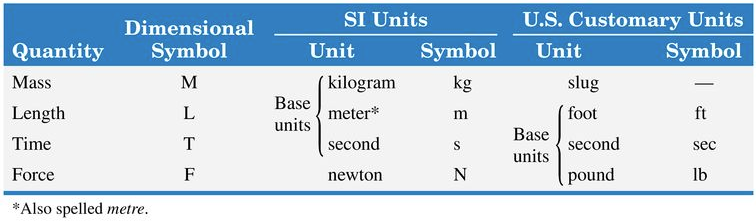
\includegraphics[width=0.5\linewidth,height=\textheight,keepaspectratio]{preliminaries/../figures/units/units_table.png}

}

\caption{Source: MKB}

\end{figure}%

In this class, we will use both SI and US customary units.

In the US customary units, the pound is used both as a unit of force
(lbf) and as a unit of mass (lbm). The lbm is the amount of mass which
weighs 1 lbf under standard conditions (at latitude 45° and sea level).
In MKB, almost exclusively the unit of slug is used for mass. In
addition, they use the symbol lb to mean pound force.

Notice that seconds is abbreviated as s in SI units and sec in US
customary units.

For the gravitational acceleration use the values \(g = 9.81\) m
s\(^{-2}\) in SI units and \(g = 32.2\) ft sec\(^{-2}\) in US customary
units.

\begin{tcolorbox}[enhanced jigsaw, arc=.35mm, bottomrule=.15mm, bottomtitle=1mm, breakable, colback=white, colbacktitle=quarto-callout-important-color!10!white, colframe=quarto-callout-important-color-frame, coltitle=black, left=2mm, leftrule=.75mm, opacityback=0, opacitybacktitle=0.6, rightrule=.15mm, title=\textcolor{quarto-callout-important-color}{\faExclamation}\hspace{0.5em}{Note!}, titlerule=0mm, toprule=.15mm, toptitle=1mm]

When solving a problem, keep all variables in the unit system they are
given. For example, you may convert g to kg, but don't convert g to
slugs!

\end{tcolorbox}

\section{Summary}\label{summary}

In U.S. customary units, the \textbf{slug} is the unit of mass: \(1\)
slug \(= 1\) lb\(\cdot\)sec\(^2\)/ft. Use \(g = 32.2\) ft/sec\(^2\) in
U.S. customary units and \(g = 9.81\) m/s\(^2\) in SI. Keep all
variables in the unit system they are given.

\section{Exercises}\label{exercises}

\emph{The following problems are from Set 02 -- Units.}

\textbf{1.} {[}MKB 1/2{]} Familiarise yourself with the U.S. unit of
mass (slugs). Note that \(1\) kg \(\approx 0.0685\) slugs. \emph{(ans.
\(W = 14\,720\) N or \(3310\) lb; \(m = 102.8\) slugs)}

\begin{figure}[H]

{\centering 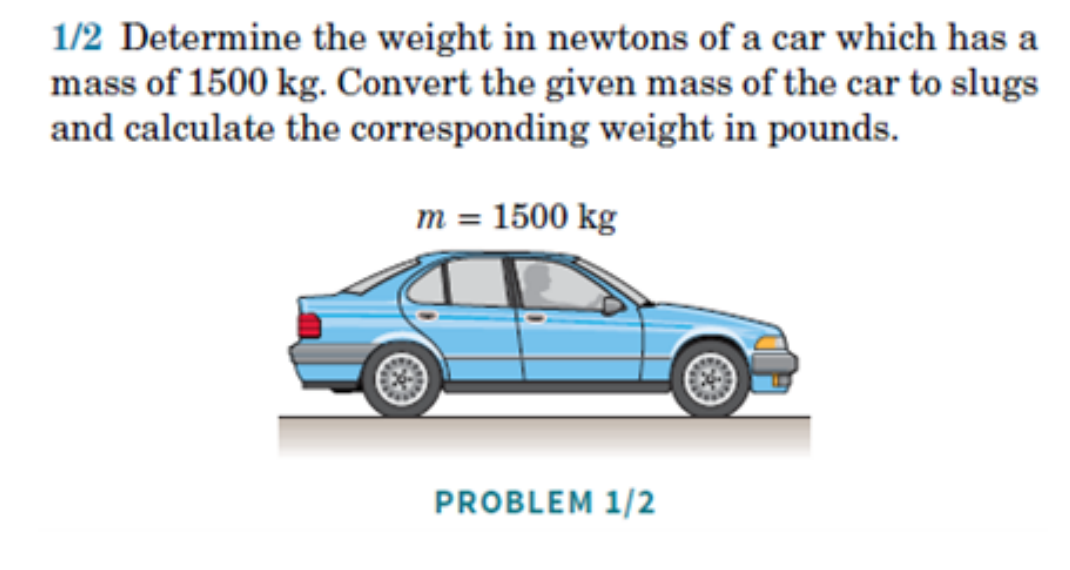
\includegraphics[width=0.5\linewidth,height=\textheight,keepaspectratio]{preliminaries/../figures/note_on_units/01-002.png}

}

\caption{MKB 1/2.}

\end{figure}%

\textbf{2.} Read
\href{https://archive.nytimes.com/www.nytimes.com/library/national/science/100199sci-nasa-mars.html}{this
article} about the Mars Climate Orbiter loss and reflect on the
importance of consistent units.

\chapter{Free Body Diagrams}\label{free-body-diagrams}

Recall the following table taken from the Hibbeler Statics textbook. It
summarizes the constraint resultant forces and moments due to various
types of supports.

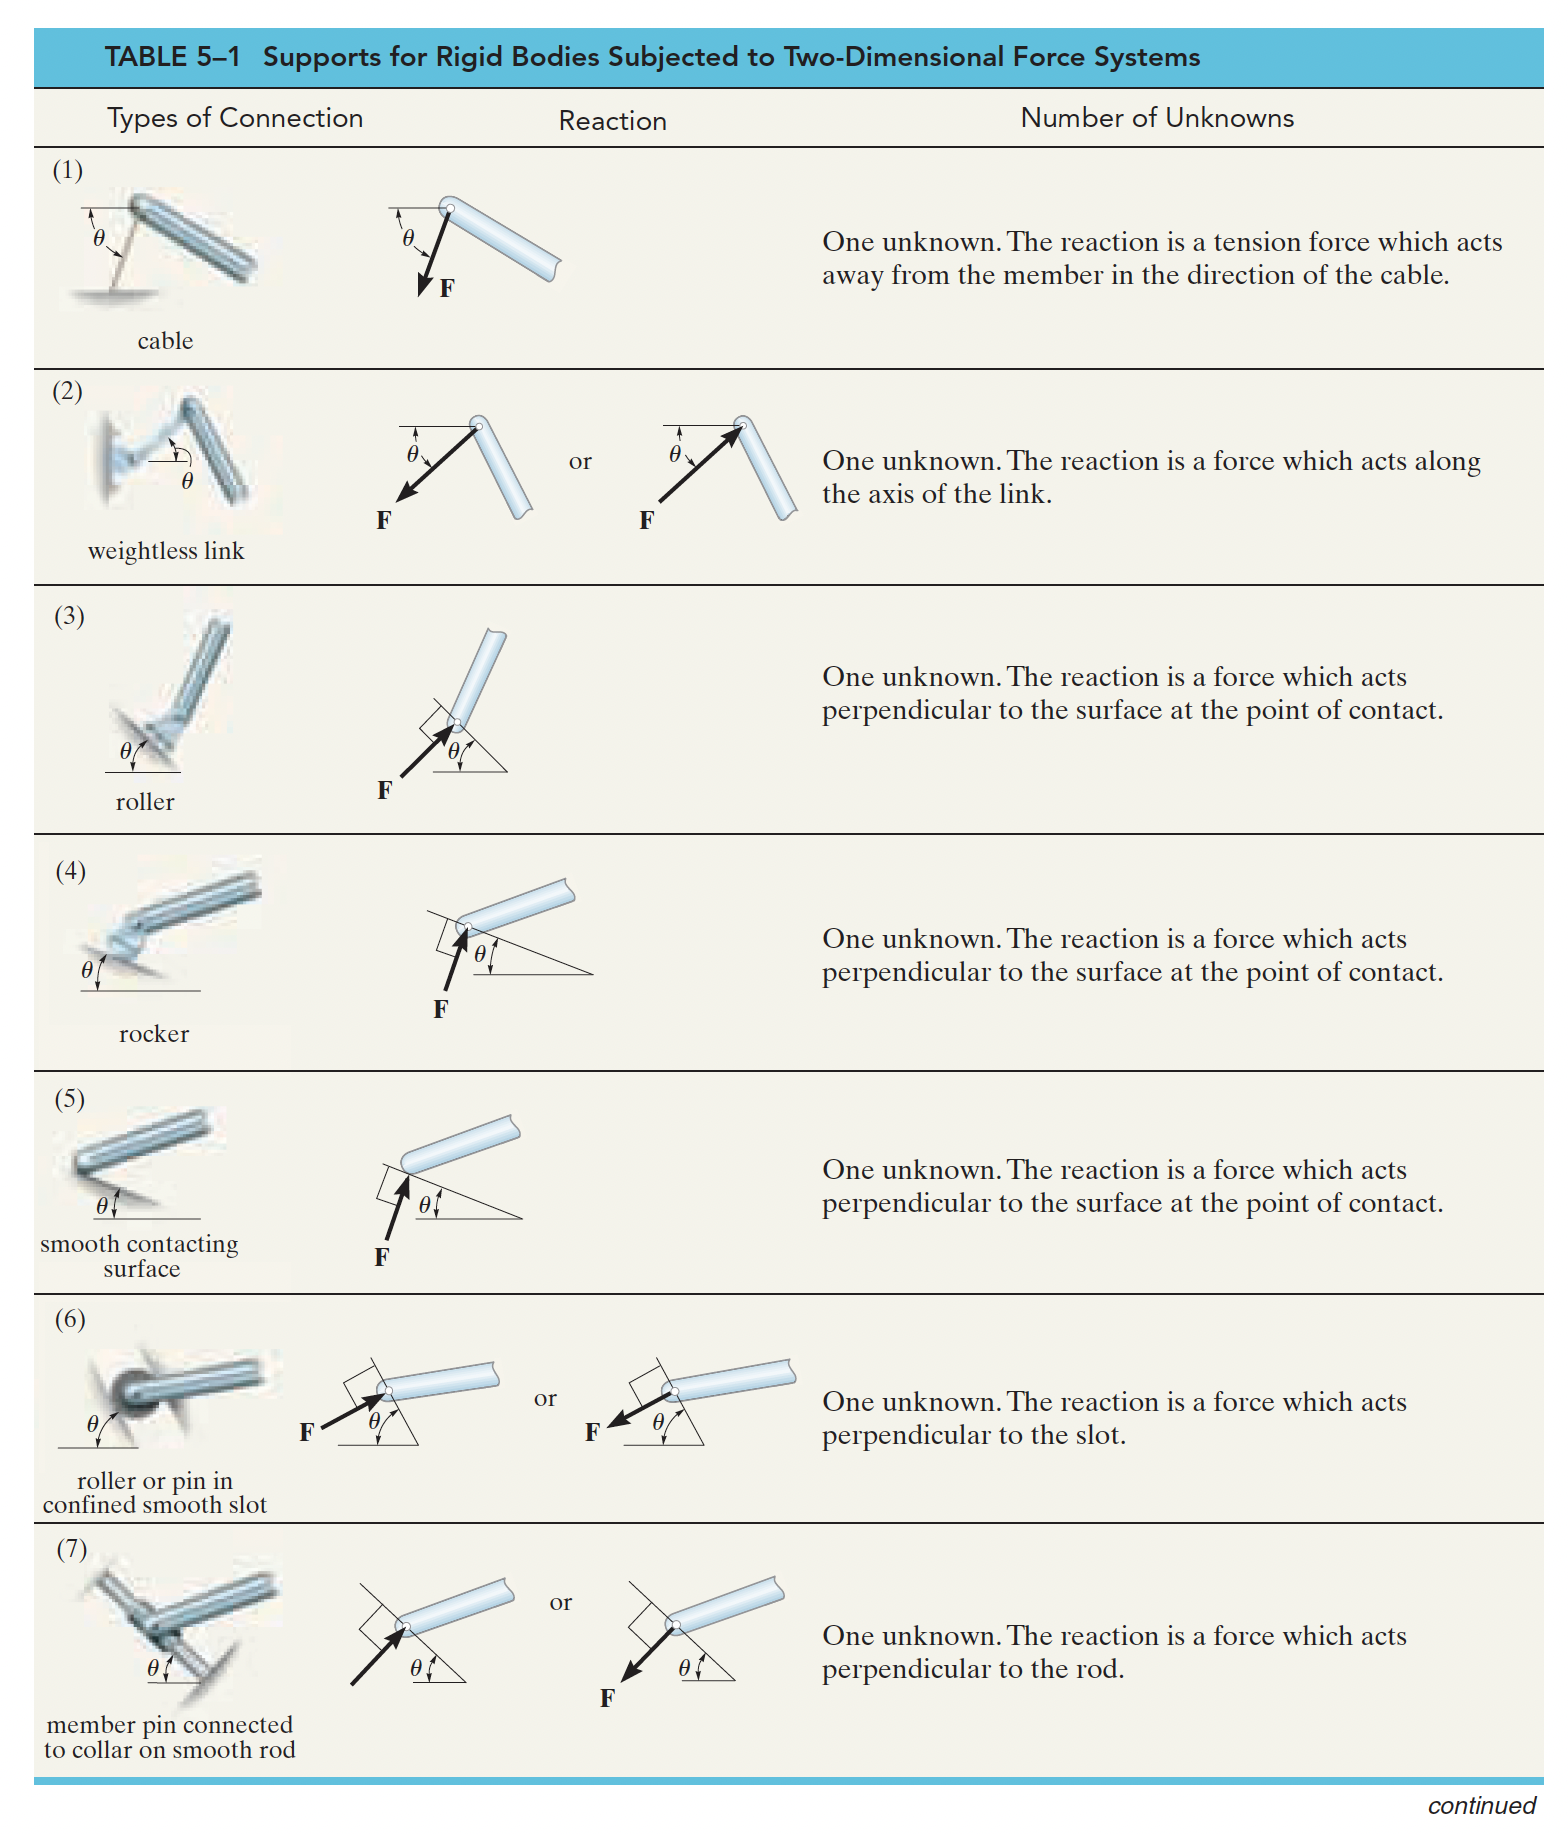
\includegraphics[width=0.8\linewidth,height=\textheight,keepaspectratio]{preliminaries/../figures/free_body_diagrams/fbd1.png}

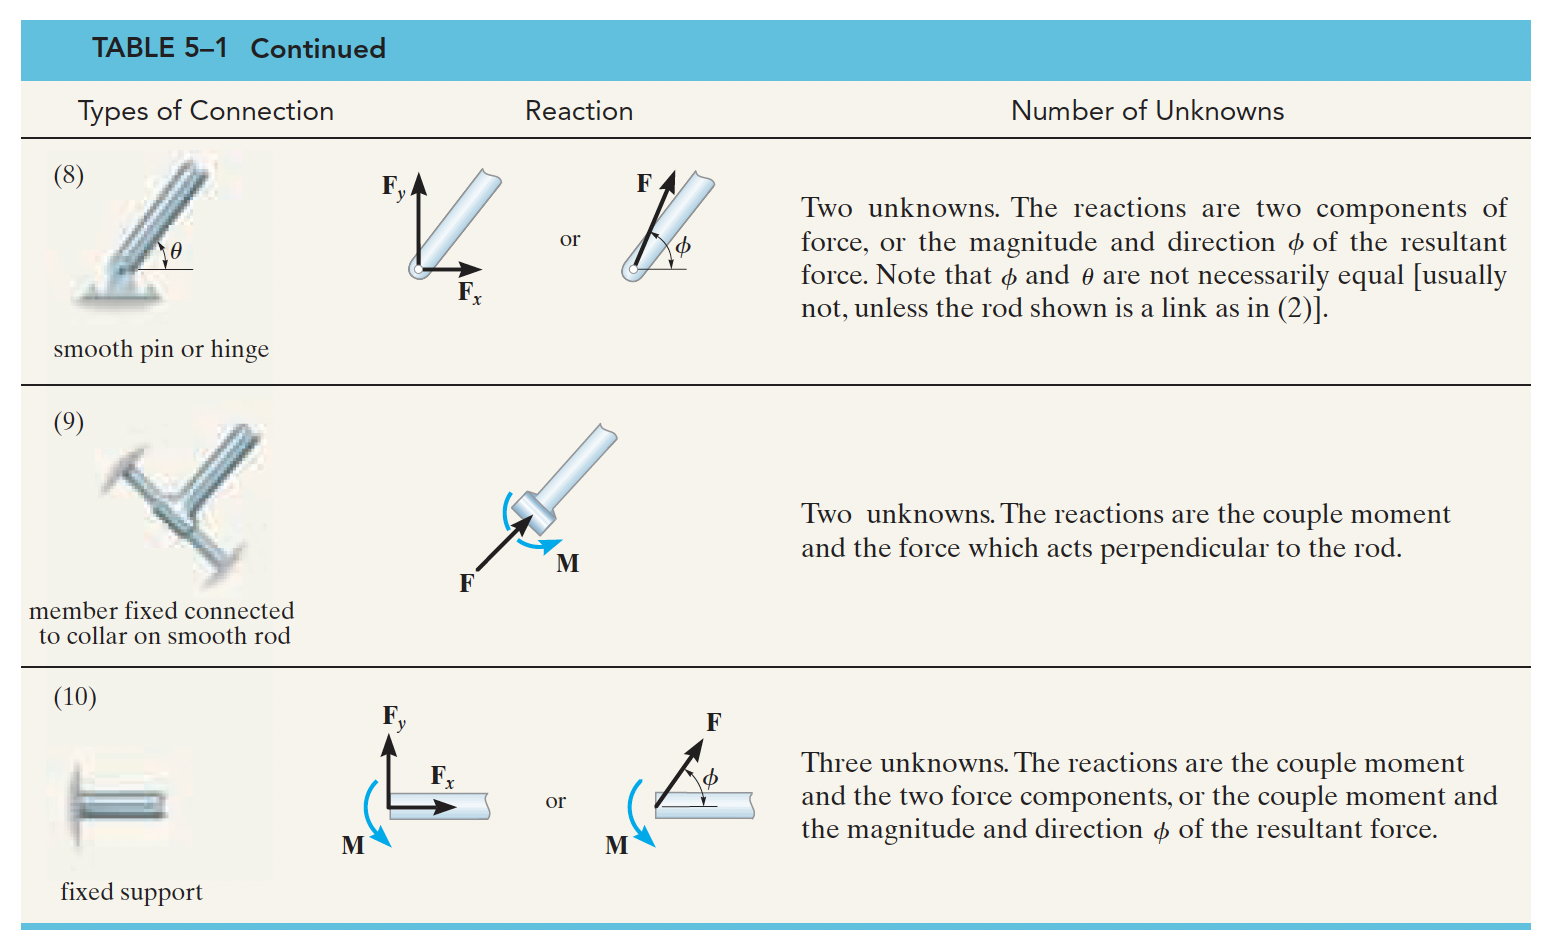
\includegraphics[width=0.8\linewidth,height=\textheight,keepaspectratio]{preliminaries/../figures/free_body_diagrams/fbd2.png}

\begin{tcolorbox}[enhanced jigsaw, arc=.35mm, bottomrule=.15mm, bottomtitle=1mm, breakable, colback=white, colbacktitle=quarto-callout-tip-color!10!white, colframe=quarto-callout-tip-color-frame, coltitle=black, left=2mm, leftrule=.75mm, opacityback=0, opacitybacktitle=0.6, rightrule=.15mm, title=\textcolor{quarto-callout-tip-color}{\faLightbulb}\hspace{0.5em}{Think!}, titlerule=0mm, toprule=.15mm, toptitle=1mm]

\textbf{Question:} What is the general rule which encompasses all the
cases in the above table and more?

\begin{quote}
\textbf{Answer}

Whenever translation in a certain direction is constrained, a constraint
force in that direction enforces the constraint. Whenever rotation along
a certain axis is constrained, a constraint moment along the same axis
results.
\end{quote}

\end{tcolorbox}

\begin{tcolorbox}[enhanced jigsaw, arc=.35mm, bottomrule=.15mm, bottomtitle=1mm, breakable, colback=white, colbacktitle=quarto-callout-important-color!10!white, colframe=quarto-callout-important-color-frame, coltitle=black, left=2mm, leftrule=.75mm, opacityback=0, opacitybacktitle=0.6, rightrule=.15mm, title=\textcolor{quarto-callout-important-color}{\faExclamation}\hspace{0.5em}{Note! Notation}, titlerule=0mm, toprule=.15mm, toptitle=1mm]

Good notation is important: in print, vectors are usually denoted by
boldface, e.g.~\({\bf v}\) or \({\bf F}\). In writing, vectors are
either denoted by an overhead arrow, e.g.~\(\vec{v}\), or by a line or
squiggle underneath, e.g.~\(\underline{v}\). We opt for the latter
notation since we reserve the top of a vector for other accents.

\end{tcolorbox}

For a massless inextensible string, the tension is the same at all
points along the string.

For a frictionless massless pulley, the tension in the string on either
side of the pulley is the same.

\section{Exercises}\label{exercises-1}

\emph{The following problems are from Set 00 -- Free Body Diagrams.
Gravity acts vertically down; all problems are set up in the vertical
plane.}

\textbf{1.} Draw the FBD of the horizontal beam.

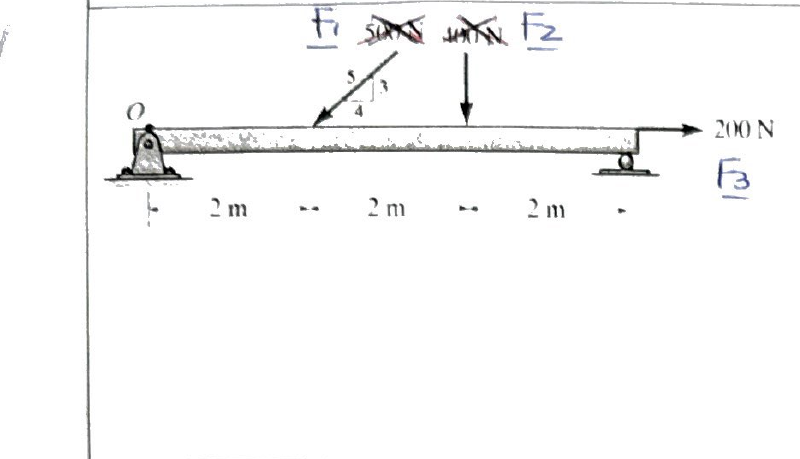
\includegraphics[width=0.5\linewidth,height=\textheight,keepaspectratio]{preliminaries/../figures/free_body_diagrams/problems/p1_setup.png}

\begin{tcolorbox}[enhanced jigsaw, arc=.35mm, bottomrule=.15mm, bottomtitle=1mm, breakable, colback=white, colbacktitle=quarto-callout-note-color!10!white, colframe=quarto-callout-note-color-frame, coltitle=black, left=2mm, leftrule=.75mm, opacityback=0, opacitybacktitle=0.6, rightrule=.15mm, title=\textcolor{quarto-callout-note-color}{\faInfo}\hspace{0.5em}{Answer}, titlerule=0mm, toprule=.15mm, toptitle=1mm]

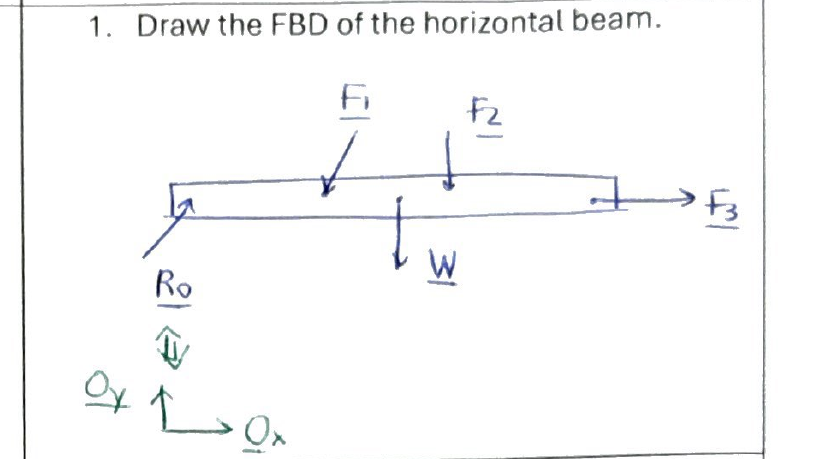
\includegraphics[width=0.5\linewidth,height=\textheight,keepaspectratio]{preliminaries/../figures/free_body_diagrams/problems/p1_fbd.png}

\end{tcolorbox}

\textbf{2.} Draw the FBD of the horizontal beam.

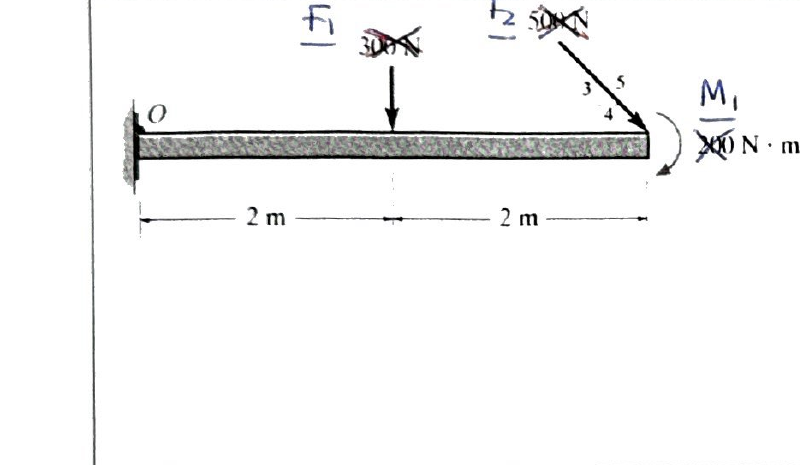
\includegraphics[width=0.5\linewidth,height=\textheight,keepaspectratio]{preliminaries/../figures/free_body_diagrams/problems/p2_setup.png}

\begin{tcolorbox}[enhanced jigsaw, arc=.35mm, bottomrule=.15mm, bottomtitle=1mm, breakable, colback=white, colbacktitle=quarto-callout-note-color!10!white, colframe=quarto-callout-note-color-frame, coltitle=black, left=2mm, leftrule=.75mm, opacityback=0, opacitybacktitle=0.6, rightrule=.15mm, title=\textcolor{quarto-callout-note-color}{\faInfo}\hspace{0.5em}{Answer}, titlerule=0mm, toprule=.15mm, toptitle=1mm]

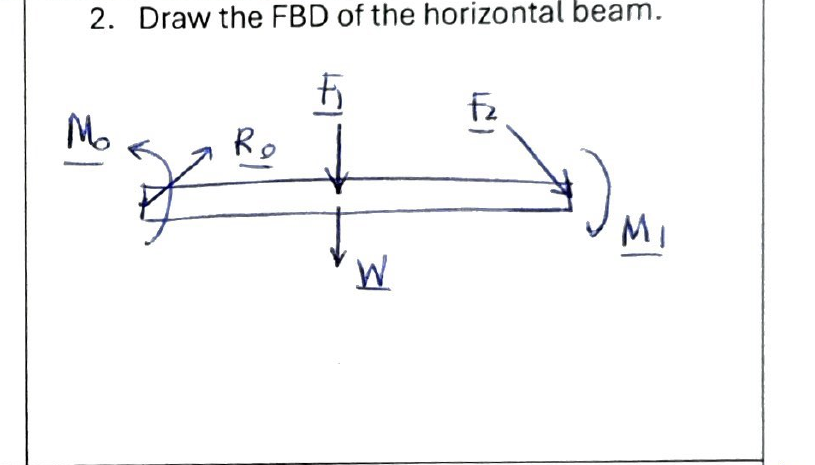
\includegraphics[width=0.5\linewidth,height=\textheight,keepaspectratio]{preliminaries/../figures/free_body_diagrams/problems/p2_fbd.png}

\end{tcolorbox}

\textbf{3.} Draw the FBD of angled beam \(AB\).

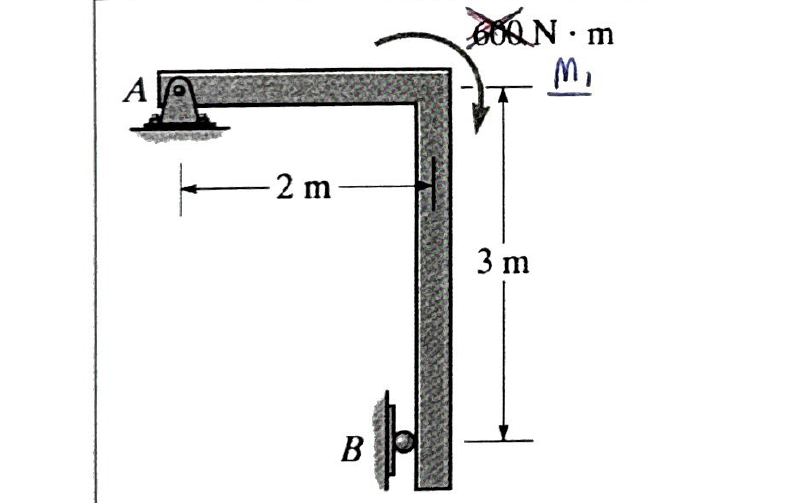
\includegraphics[width=0.5\linewidth,height=\textheight,keepaspectratio]{preliminaries/../figures/free_body_diagrams/problems/p3_setup.png}

\begin{tcolorbox}[enhanced jigsaw, arc=.35mm, bottomrule=.15mm, bottomtitle=1mm, breakable, colback=white, colbacktitle=quarto-callout-note-color!10!white, colframe=quarto-callout-note-color-frame, coltitle=black, left=2mm, leftrule=.75mm, opacityback=0, opacitybacktitle=0.6, rightrule=.15mm, title=\textcolor{quarto-callout-note-color}{\faInfo}\hspace{0.5em}{Answer}, titlerule=0mm, toprule=.15mm, toptitle=1mm]

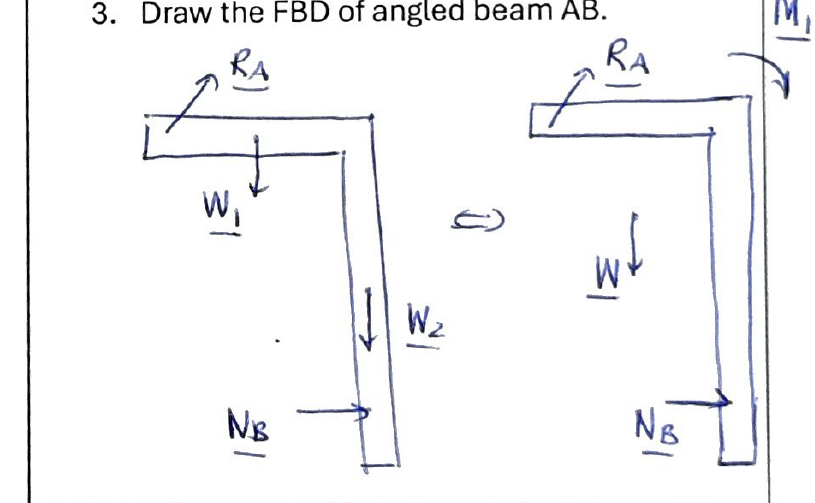
\includegraphics[width=0.5\linewidth,height=\textheight,keepaspectratio]{preliminaries/../figures/free_body_diagrams/problems/p3_fbd.png}

\end{tcolorbox}

\textbf{4.} Draw the FBD of the bar.

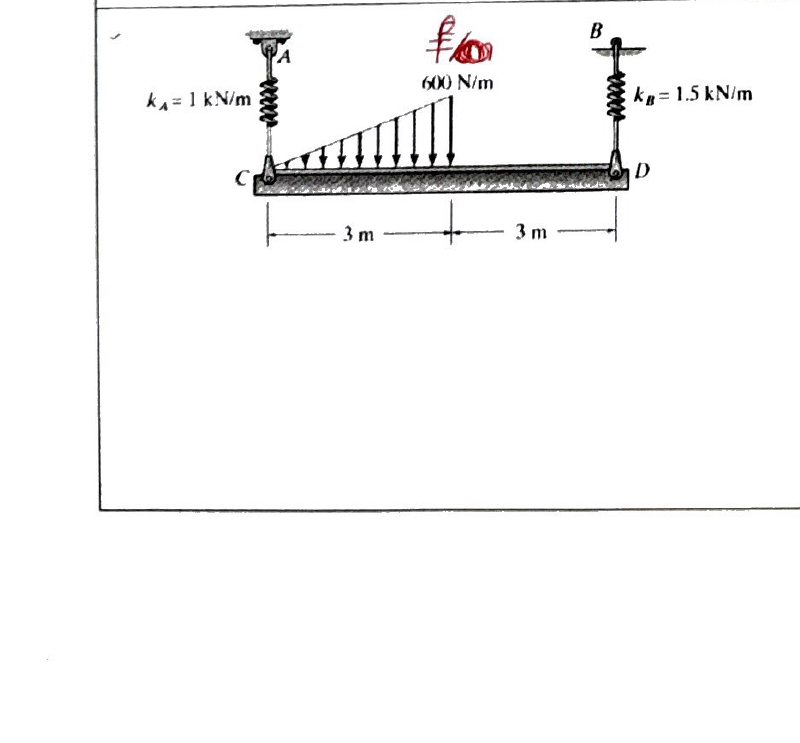
\includegraphics[width=0.5\linewidth,height=\textheight,keepaspectratio]{preliminaries/../figures/free_body_diagrams/problems/p4_setup.png}

\begin{tcolorbox}[enhanced jigsaw, arc=.35mm, bottomrule=.15mm, bottomtitle=1mm, breakable, colback=white, colbacktitle=quarto-callout-note-color!10!white, colframe=quarto-callout-note-color-frame, coltitle=black, left=2mm, leftrule=.75mm, opacityback=0, opacitybacktitle=0.6, rightrule=.15mm, title=\textcolor{quarto-callout-note-color}{\faInfo}\hspace{0.5em}{Answer}, titlerule=0mm, toprule=.15mm, toptitle=1mm]

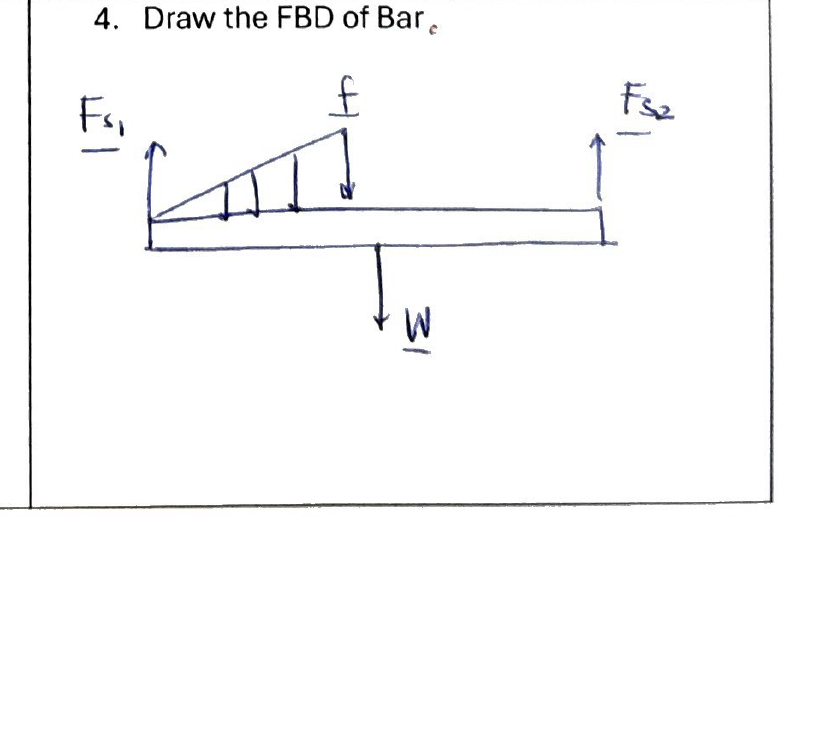
\includegraphics[width=0.5\linewidth,height=\textheight,keepaspectratio]{preliminaries/../figures/free_body_diagrams/problems/p4_fbd.png}

\end{tcolorbox}

\textbf{5.} Draw the FBD of beam \(AB\).

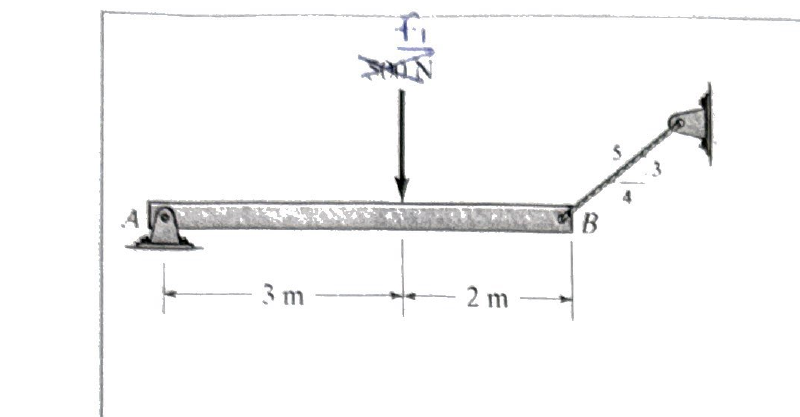
\includegraphics[width=0.5\linewidth,height=\textheight,keepaspectratio]{preliminaries/../figures/free_body_diagrams/problems/p5_setup.png}

\begin{tcolorbox}[enhanced jigsaw, arc=.35mm, bottomrule=.15mm, bottomtitle=1mm, breakable, colback=white, colbacktitle=quarto-callout-note-color!10!white, colframe=quarto-callout-note-color-frame, coltitle=black, left=2mm, leftrule=.75mm, opacityback=0, opacitybacktitle=0.6, rightrule=.15mm, title=\textcolor{quarto-callout-note-color}{\faInfo}\hspace{0.5em}{Answer}, titlerule=0mm, toprule=.15mm, toptitle=1mm]

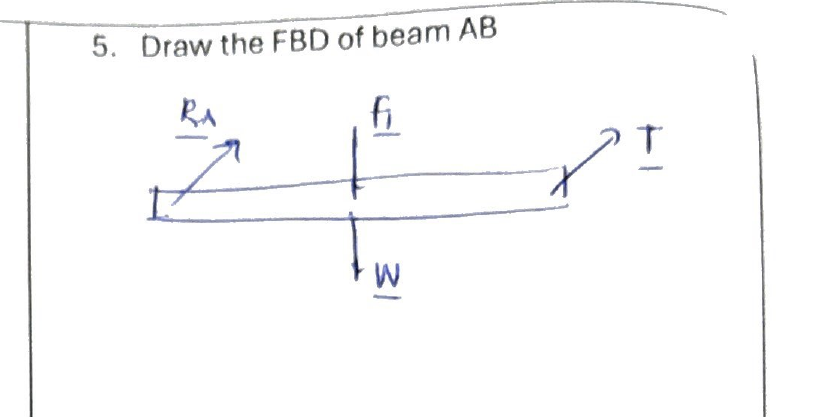
\includegraphics[width=0.5\linewidth,height=\textheight,keepaspectratio]{preliminaries/../figures/free_body_diagrams/problems/p5_fbd.png}

\end{tcolorbox}

\textbf{6.} Draw the FBDs of disks \(A\) and \(B\) each separately.

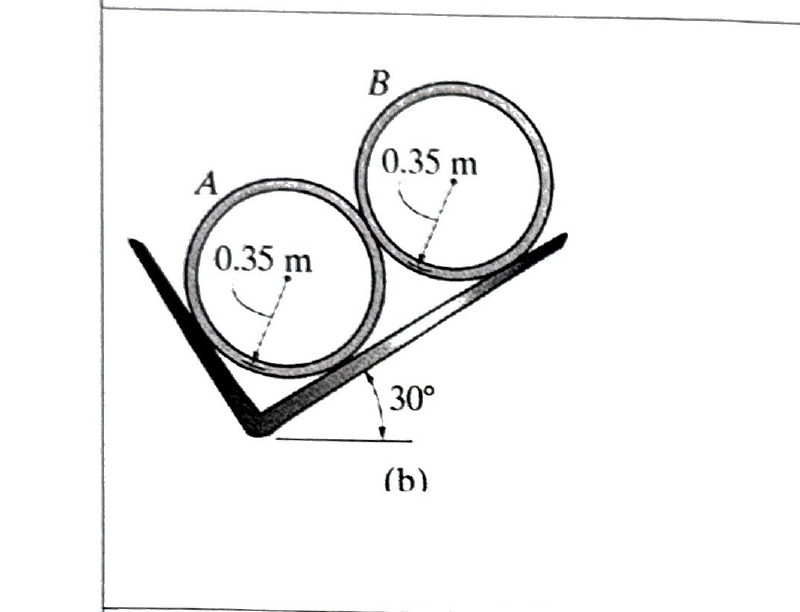
\includegraphics[width=0.5\linewidth,height=\textheight,keepaspectratio]{preliminaries/../figures/free_body_diagrams/problems/p6_setup.png}

\begin{tcolorbox}[enhanced jigsaw, arc=.35mm, bottomrule=.15mm, bottomtitle=1mm, breakable, colback=white, colbacktitle=quarto-callout-note-color!10!white, colframe=quarto-callout-note-color-frame, coltitle=black, left=2mm, leftrule=.75mm, opacityback=0, opacitybacktitle=0.6, rightrule=.15mm, title=\textcolor{quarto-callout-note-color}{\faInfo}\hspace{0.5em}{Answer}, titlerule=0mm, toprule=.15mm, toptitle=1mm]

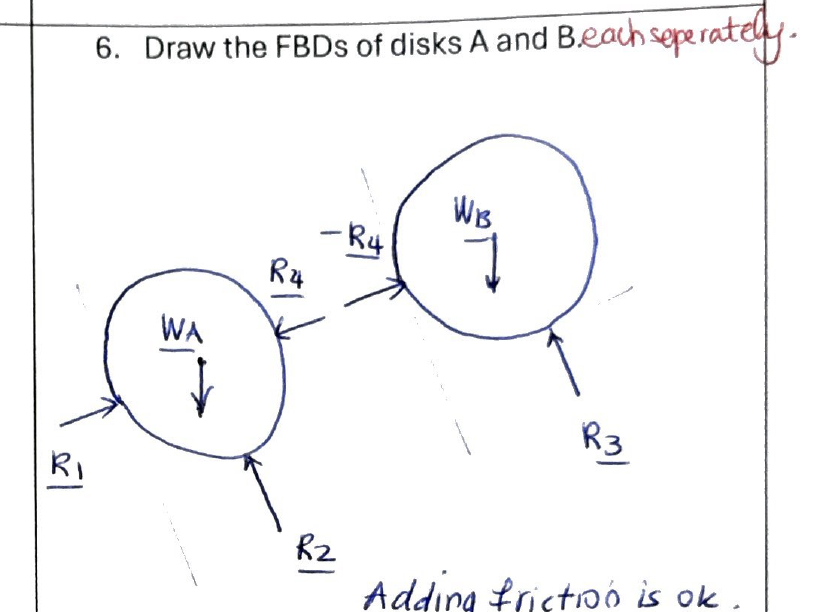
\includegraphics[width=0.5\linewidth,height=\textheight,keepaspectratio]{preliminaries/../figures/free_body_diagrams/problems/p6_fbd.png}

\end{tcolorbox}

\textbf{7.} Draw the FBD of the bar.

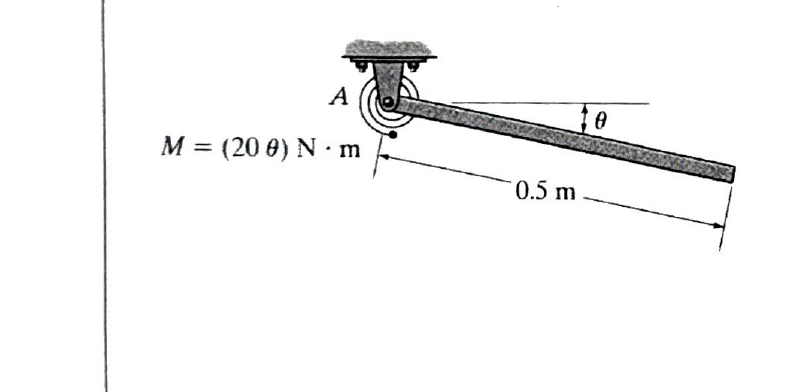
\includegraphics[width=0.5\linewidth,height=\textheight,keepaspectratio]{preliminaries/../figures/free_body_diagrams/problems/p7_setup.png}

\begin{tcolorbox}[enhanced jigsaw, arc=.35mm, bottomrule=.15mm, bottomtitle=1mm, breakable, colback=white, colbacktitle=quarto-callout-note-color!10!white, colframe=quarto-callout-note-color-frame, coltitle=black, left=2mm, leftrule=.75mm, opacityback=0, opacitybacktitle=0.6, rightrule=.15mm, title=\textcolor{quarto-callout-note-color}{\faInfo}\hspace{0.5em}{Answer}, titlerule=0mm, toprule=.15mm, toptitle=1mm]

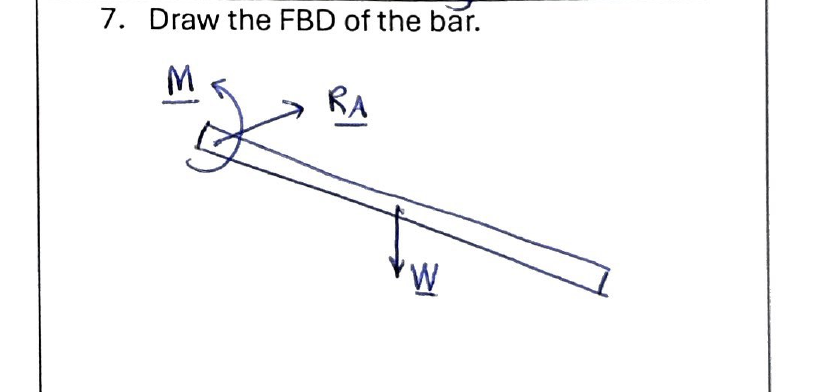
\includegraphics[width=0.5\linewidth,height=\textheight,keepaspectratio]{preliminaries/../figures/free_body_diagrams/problems/p7_fbd.png}

\end{tcolorbox}

\textbf{8.} Draw the FBD of bar \(AB\).

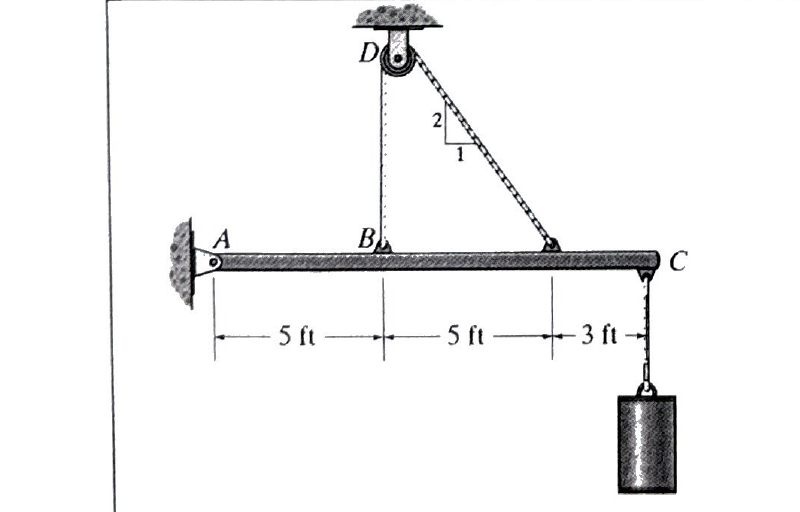
\includegraphics[width=0.5\linewidth,height=\textheight,keepaspectratio]{preliminaries/../figures/free_body_diagrams/problems/p8_setup.png}

\begin{tcolorbox}[enhanced jigsaw, arc=.35mm, bottomrule=.15mm, bottomtitle=1mm, breakable, colback=white, colbacktitle=quarto-callout-note-color!10!white, colframe=quarto-callout-note-color-frame, coltitle=black, left=2mm, leftrule=.75mm, opacityback=0, opacitybacktitle=0.6, rightrule=.15mm, title=\textcolor{quarto-callout-note-color}{\faInfo}\hspace{0.5em}{Answer}, titlerule=0mm, toprule=.15mm, toptitle=1mm]

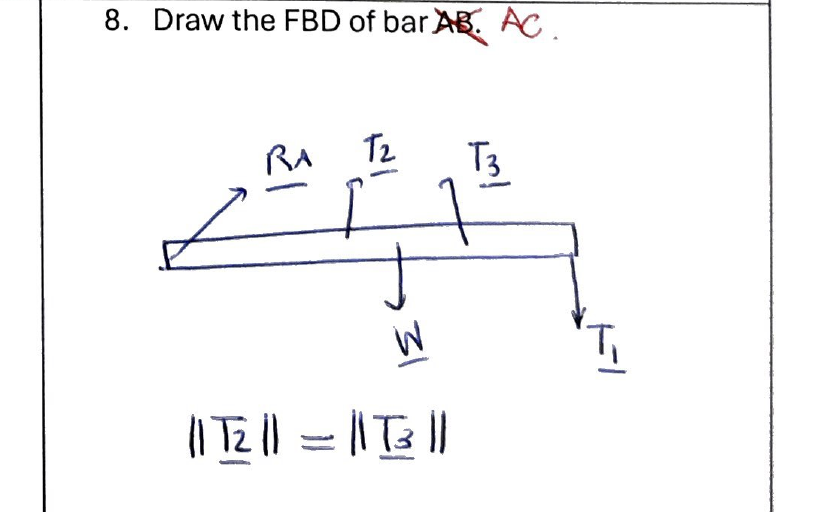
\includegraphics[width=0.5\linewidth,height=\textheight,keepaspectratio]{preliminaries/../figures/free_body_diagrams/problems/p8_fbd.png}

\end{tcolorbox}

\textbf{9.} Draw the FBD of the horizontal beam. What are the forces
acting at \(A\) and \(B\)?

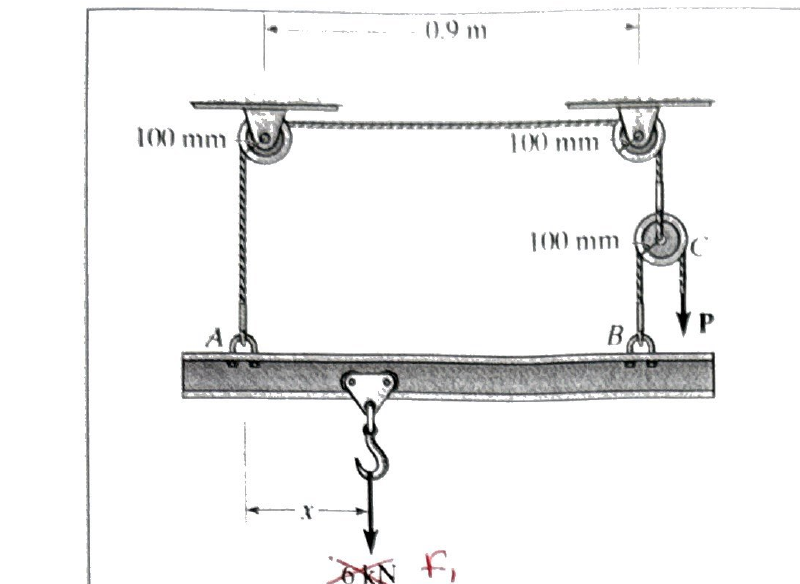
\includegraphics[width=0.5\linewidth,height=\textheight,keepaspectratio]{preliminaries/../figures/free_body_diagrams/problems/p9_setup.png}

\begin{tcolorbox}[enhanced jigsaw, arc=.35mm, bottomrule=.15mm, bottomtitle=1mm, breakable, colback=white, colbacktitle=quarto-callout-note-color!10!white, colframe=quarto-callout-note-color-frame, coltitle=black, left=2mm, leftrule=.75mm, opacityback=0, opacitybacktitle=0.6, rightrule=.15mm, title=\textcolor{quarto-callout-note-color}{\faInfo}\hspace{0.5em}{Answer}, titlerule=0mm, toprule=.15mm, toptitle=1mm]

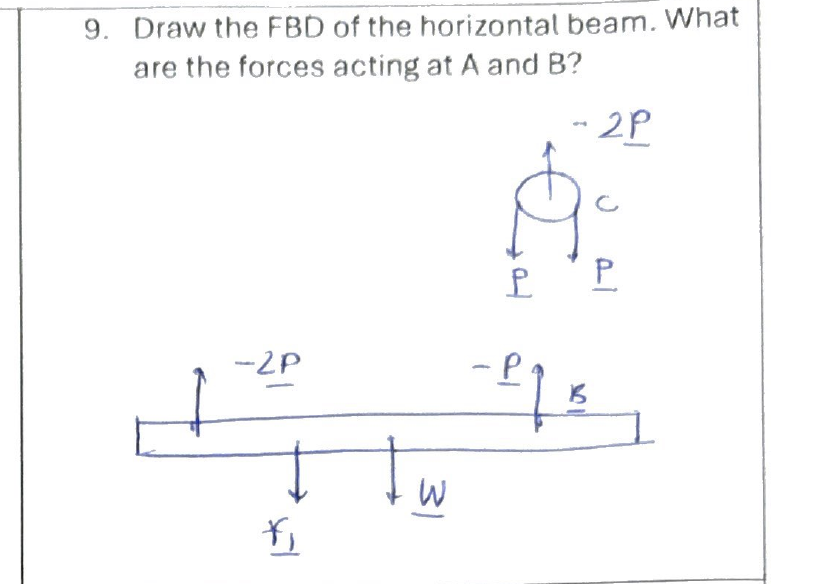
\includegraphics[width=0.5\linewidth,height=\textheight,keepaspectratio]{preliminaries/../figures/free_body_diagrams/problems/p9_fbd.png}

\end{tcolorbox}

\textbf{10.} The cylinder of mass \(m\) is in equilibrium. What forces
act on it? Gravity acts vertically downwards (same direction as the
drawn force \(\mathbf{P}\)).

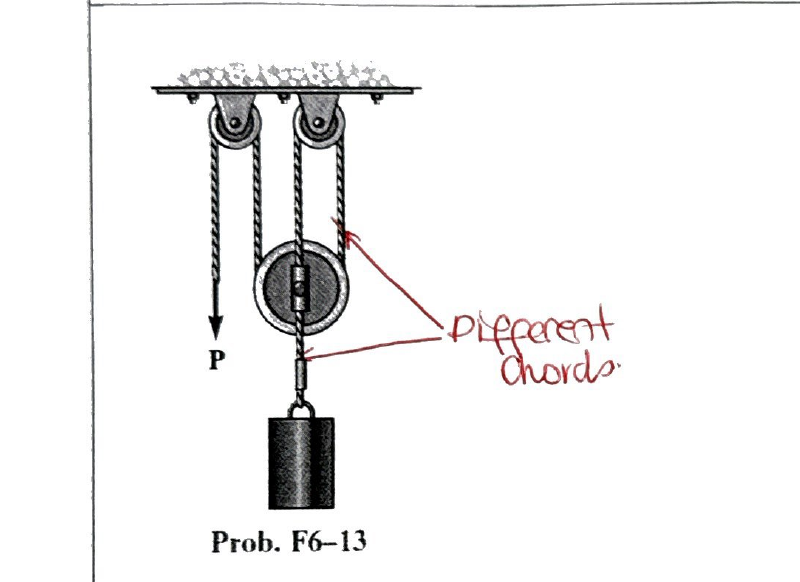
\includegraphics[width=0.5\linewidth,height=\textheight,keepaspectratio]{preliminaries/../figures/free_body_diagrams/problems/p10_setup.png}

\begin{tcolorbox}[enhanced jigsaw, arc=.35mm, bottomrule=.15mm, bottomtitle=1mm, breakable, colback=white, colbacktitle=quarto-callout-note-color!10!white, colframe=quarto-callout-note-color-frame, coltitle=black, left=2mm, leftrule=.75mm, opacityback=0, opacitybacktitle=0.6, rightrule=.15mm, title=\textcolor{quarto-callout-note-color}{\faInfo}\hspace{0.5em}{Answer}, titlerule=0mm, toprule=.15mm, toptitle=1mm]

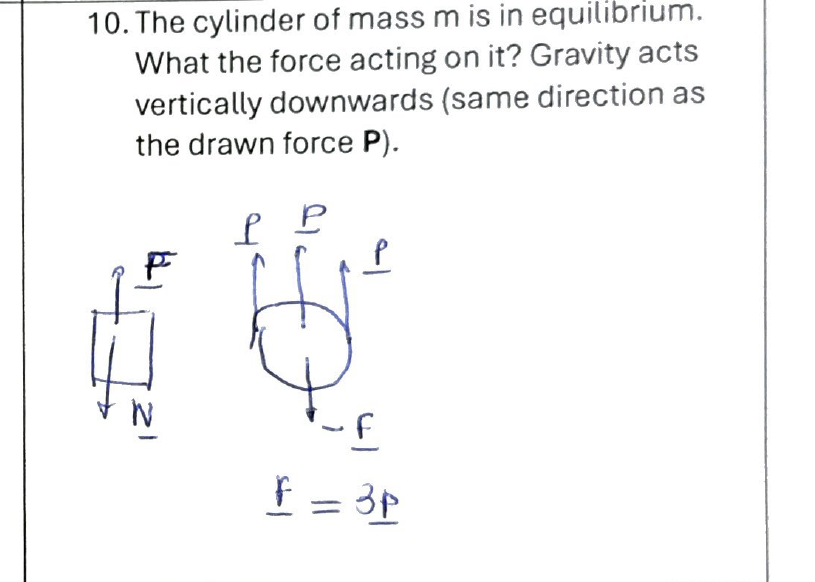
\includegraphics[width=0.5\linewidth,height=\textheight,keepaspectratio]{preliminaries/../figures/free_body_diagrams/problems/p10_fbd.png}

\end{tcolorbox}

\textbf{11.} Draw the FBD of the beam.

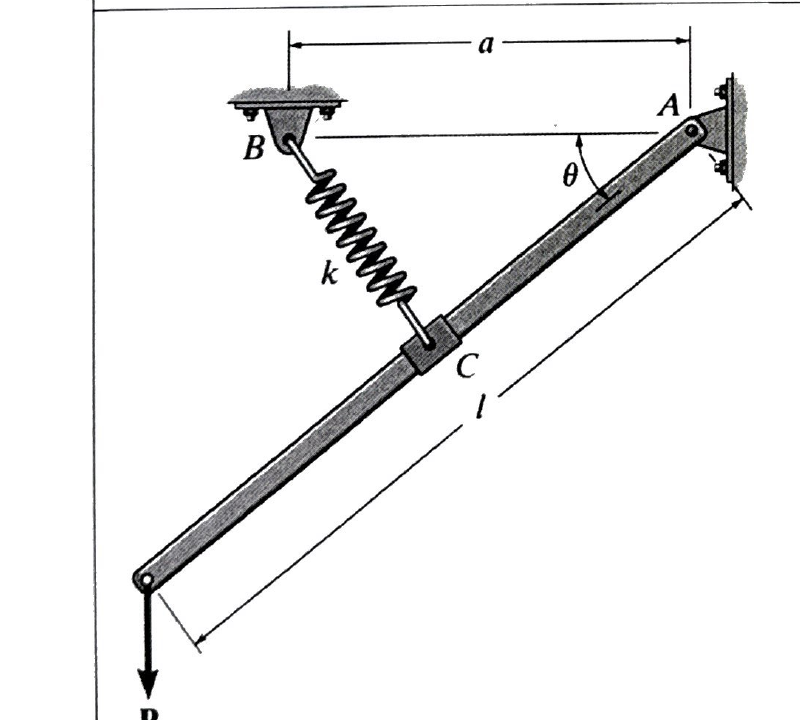
\includegraphics[width=0.5\linewidth,height=\textheight,keepaspectratio]{preliminaries/../figures/free_body_diagrams/problems/p11_setup.png}

\begin{tcolorbox}[enhanced jigsaw, arc=.35mm, bottomrule=.15mm, bottomtitle=1mm, breakable, colback=white, colbacktitle=quarto-callout-note-color!10!white, colframe=quarto-callout-note-color-frame, coltitle=black, left=2mm, leftrule=.75mm, opacityback=0, opacitybacktitle=0.6, rightrule=.15mm, title=\textcolor{quarto-callout-note-color}{\faInfo}\hspace{0.5em}{Answer}, titlerule=0mm, toprule=.15mm, toptitle=1mm]

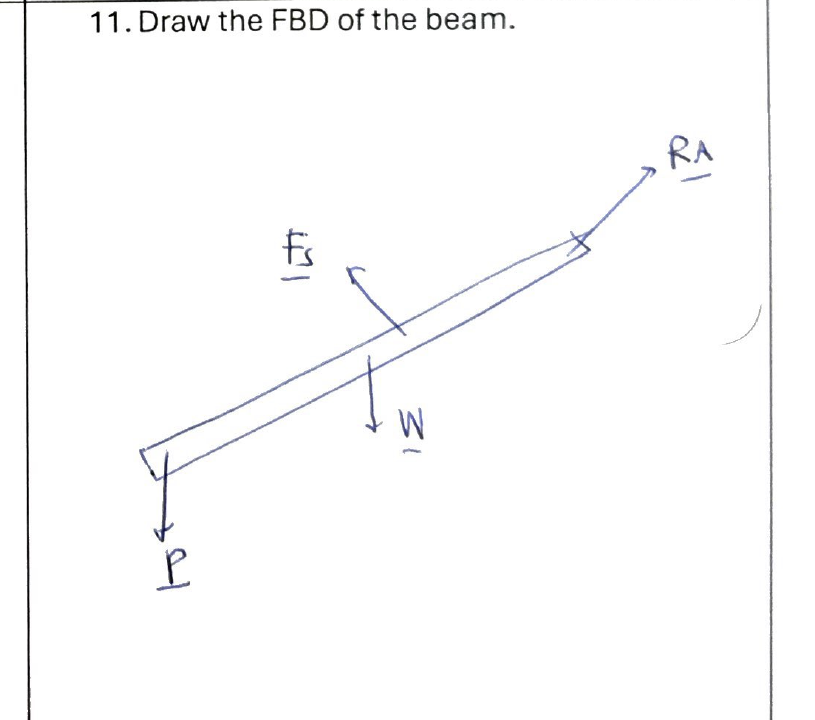
\includegraphics[width=0.5\linewidth,height=\textheight,keepaspectratio]{preliminaries/../figures/free_body_diagrams/problems/p11_fbd.png}

\end{tcolorbox}

\textbf{12.} Draw the FBDs of bars \(AB\) and \(BC\).

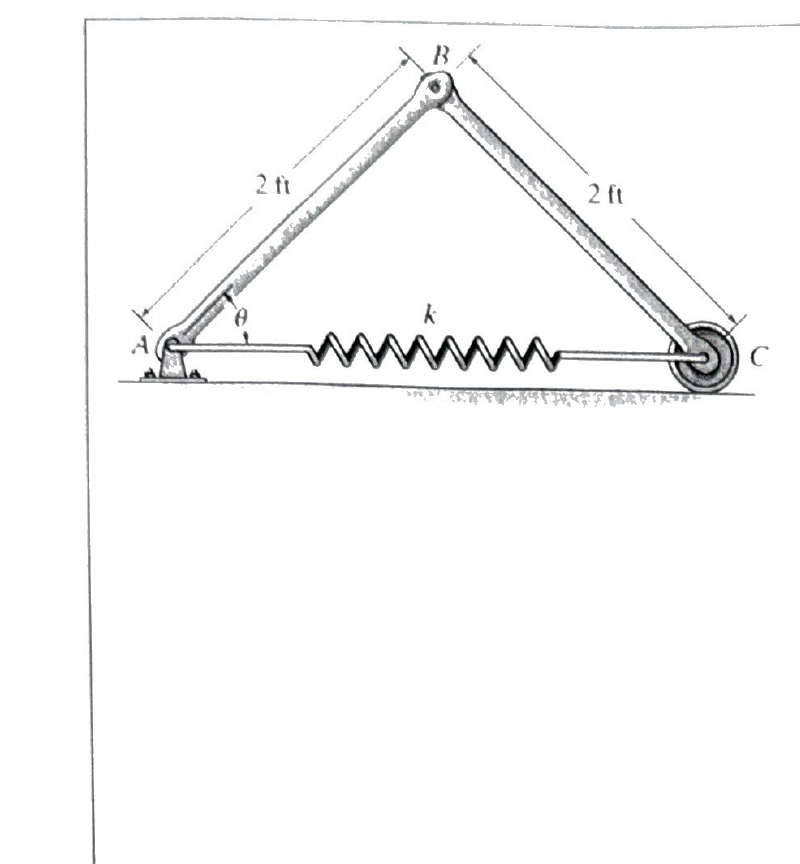
\includegraphics[width=0.5\linewidth,height=\textheight,keepaspectratio]{preliminaries/../figures/free_body_diagrams/problems/p12_setup.png}

\begin{tcolorbox}[enhanced jigsaw, arc=.35mm, bottomrule=.15mm, bottomtitle=1mm, breakable, colback=white, colbacktitle=quarto-callout-note-color!10!white, colframe=quarto-callout-note-color-frame, coltitle=black, left=2mm, leftrule=.75mm, opacityback=0, opacitybacktitle=0.6, rightrule=.15mm, title=\textcolor{quarto-callout-note-color}{\faInfo}\hspace{0.5em}{Answer}, titlerule=0mm, toprule=.15mm, toptitle=1mm]

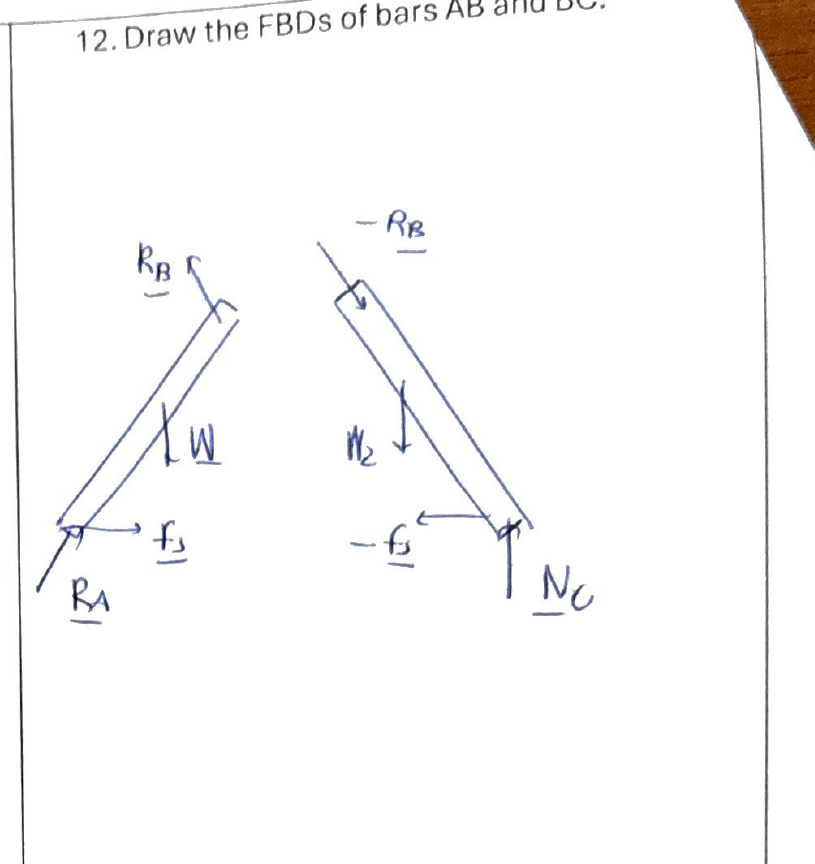
\includegraphics[width=0.5\linewidth,height=\textheight,keepaspectratio]{preliminaries/../figures/free_body_diagrams/problems/p12_fbd.png}

\end{tcolorbox}

\textbf{13.} Draw the FBDs of bars \(AC\) and \(ED\).

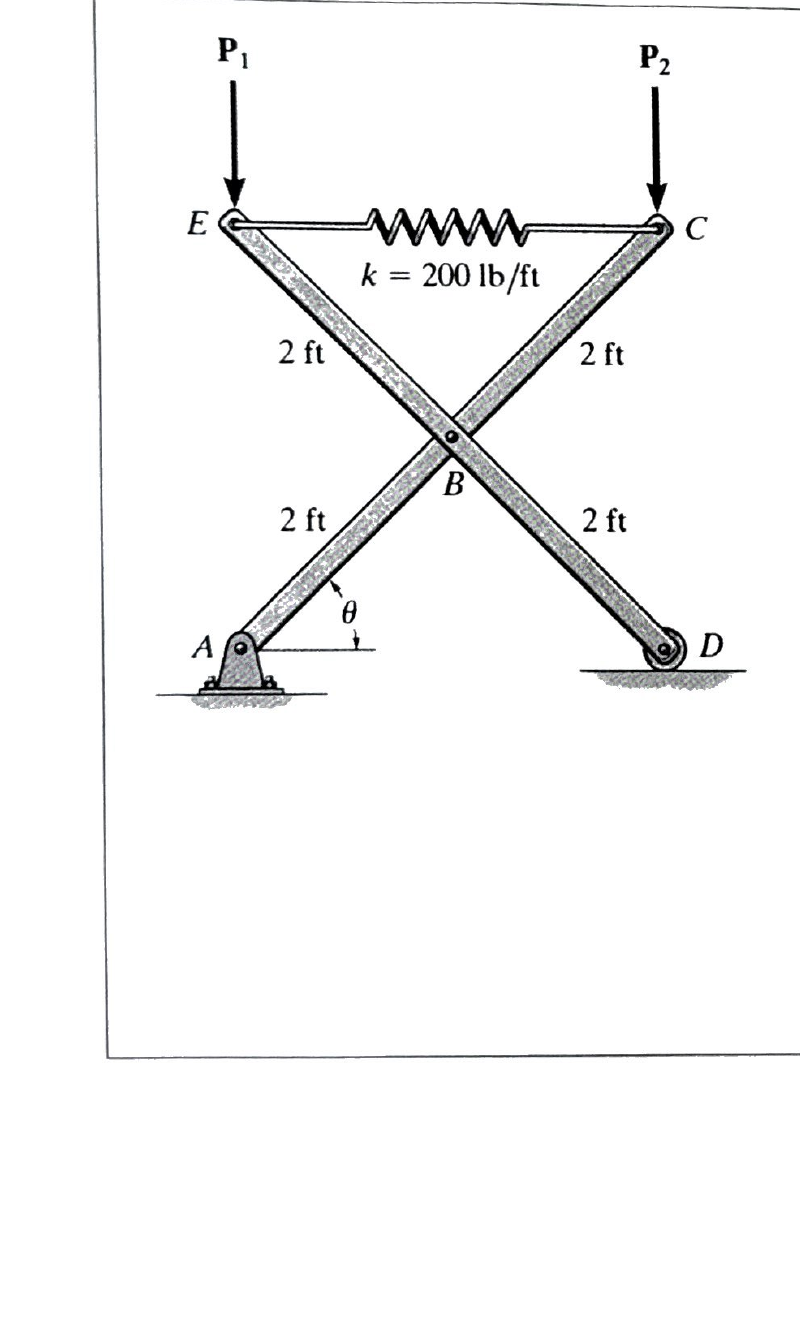
\includegraphics[width=0.5\linewidth,height=\textheight,keepaspectratio]{preliminaries/../figures/free_body_diagrams/problems/p13_setup.png}

\begin{tcolorbox}[enhanced jigsaw, arc=.35mm, bottomrule=.15mm, bottomtitle=1mm, breakable, colback=white, colbacktitle=quarto-callout-note-color!10!white, colframe=quarto-callout-note-color-frame, coltitle=black, left=2mm, leftrule=.75mm, opacityback=0, opacitybacktitle=0.6, rightrule=.15mm, title=\textcolor{quarto-callout-note-color}{\faInfo}\hspace{0.5em}{Answer}, titlerule=0mm, toprule=.15mm, toptitle=1mm]

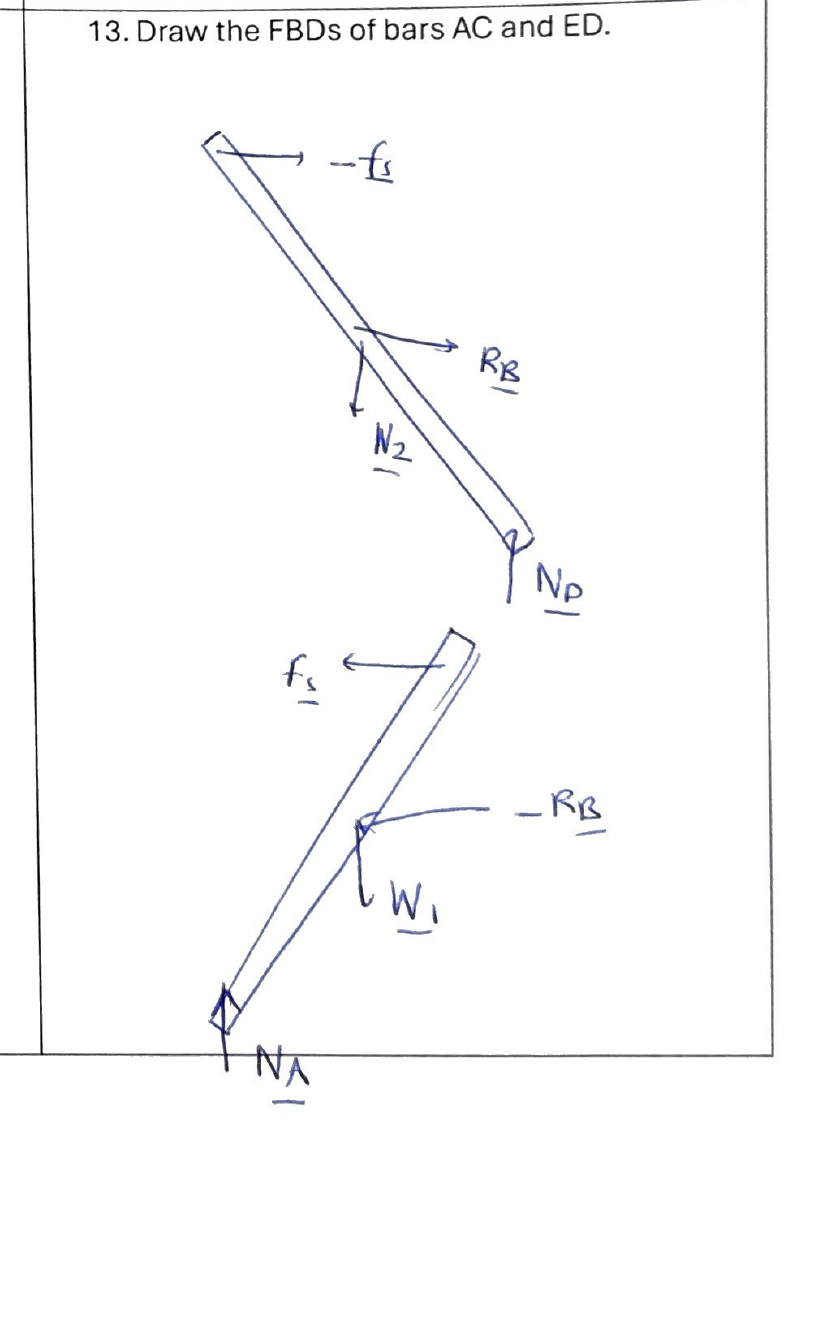
\includegraphics[width=0.5\linewidth,height=\textheight,keepaspectratio]{preliminaries/../figures/free_body_diagrams/problems/p13_fbd.png}

\end{tcolorbox}

\textbf{14.} Draw the FBD of each pulley.

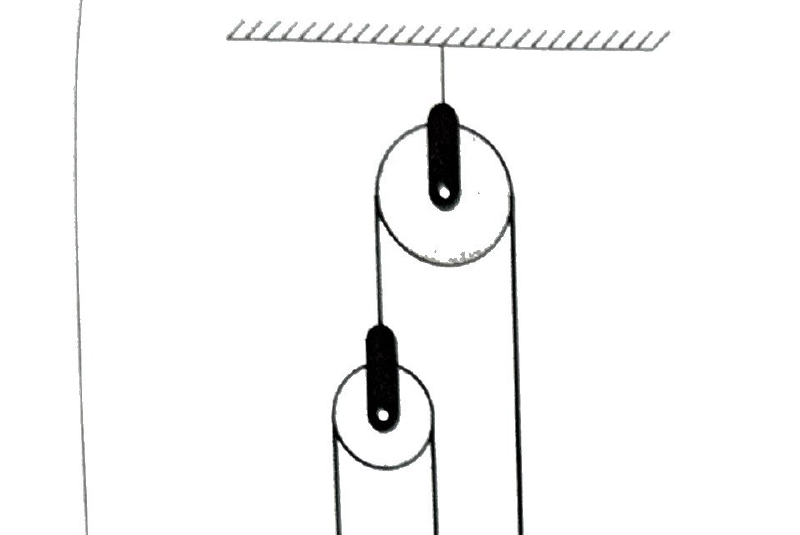
\includegraphics[width=0.5\linewidth,height=\textheight,keepaspectratio]{preliminaries/../figures/free_body_diagrams/problems/p14_setup.png}

\begin{tcolorbox}[enhanced jigsaw, arc=.35mm, bottomrule=.15mm, bottomtitle=1mm, breakable, colback=white, colbacktitle=quarto-callout-note-color!10!white, colframe=quarto-callout-note-color-frame, coltitle=black, left=2mm, leftrule=.75mm, opacityback=0, opacitybacktitle=0.6, rightrule=.15mm, title=\textcolor{quarto-callout-note-color}{\faInfo}\hspace{0.5em}{Answer}, titlerule=0mm, toprule=.15mm, toptitle=1mm]

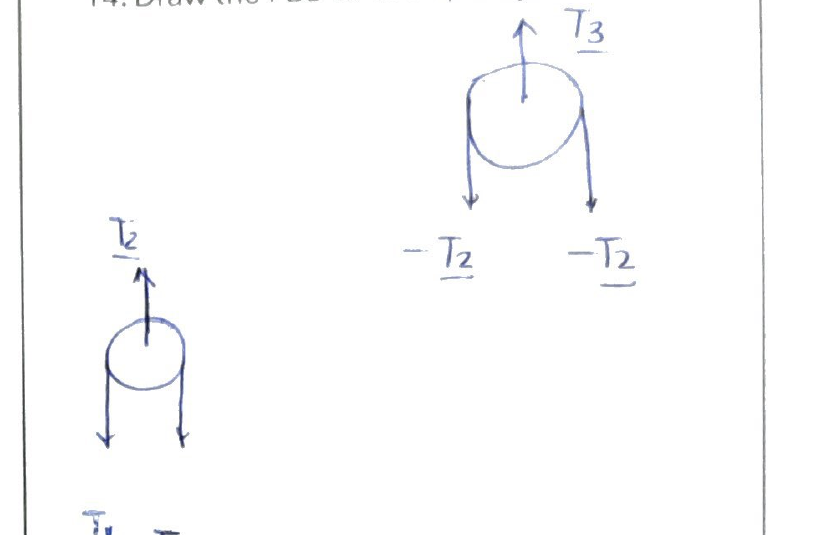
\includegraphics[width=0.5\linewidth,height=\textheight,keepaspectratio]{preliminaries/../figures/free_body_diagrams/problems/p14_fbd.png}

\end{tcolorbox}

\chapter{Vector Calculus}\label{vector-calculus}

\section{Scaling Vectors}\label{scaling-vectors}

We can scale the vector \({\bf a}\).

\begin{tcolorbox}[enhanced jigsaw, arc=.35mm, bottomrule=.15mm, bottomtitle=1mm, breakable, colback=white, colbacktitle=quarto-callout-tip-color!10!white, colframe=quarto-callout-tip-color-frame, coltitle=black, left=2mm, leftrule=.75mm, opacityback=0, opacitybacktitle=0.6, rightrule=.15mm, title=\textcolor{quarto-callout-tip-color}{\faLightbulb}\hspace{0.5em}{Think!}, titlerule=0mm, toprule=.15mm, toptitle=1mm]

Question: Consider a vector \({\bf a}\). Plot the vectors \(2{\bf a}\),
\(-{\bf a}\), \(\frac{1}{2}{\bf a}\)

\begin{quote}
\textbf{Answer}

\ldots{}
\end{quote}

\end{tcolorbox}

\begin{tcolorbox}[enhanced jigsaw, arc=.35mm, bottomrule=.15mm, bottomtitle=1mm, breakable, colback=white, colbacktitle=quarto-callout-tip-color!10!white, colframe=quarto-callout-tip-color-frame, coltitle=black, left=2mm, leftrule=.75mm, opacityback=0, opacitybacktitle=0.6, rightrule=.15mm, title=\textcolor{quarto-callout-tip-color}{\faLightbulb}\hspace{0.5em}{Think!}, titlerule=0mm, toprule=.15mm, toptitle=1mm]

Question: Give the expression for a unit vector in the direction of
\({\bf a}\)? Opposite to \({\bf a}\).

\begin{quote}
\textbf{Answer}

\begin{itemize}
\tightlist
\item
  \(\frac{\bf a}{\lnorm{\bf a}\rnorm}\) is a unit vector in the
  direction of \({\bf a}\).
\item
  \(-\frac{\bf a}{\lnorm{\bf a}\rnorm}\) is a unit vector in the
  direction opposite to that of \({\bf a}\).
\end{itemize}

\pandocbounded{
\includegraphics[keepaspectratio]{preliminaries/vector_calculus_files/figure-pdf/unnamed-chunk-1-1.pdf}}
\end{quote}

\end{tcolorbox}

\section{Vector summation and
subtraction}\label{vector-summation-and-subtraction}

Vectors can be added using the parallelogram law or by placing vectors
in a head to tail sequence.

The vector difference \({\bf a}-{\bf b}\) points from the tip of
\({\bf b}\) to the tip of \({\bf a}\).

\begin{figure}

\begin{minipage}{0.50\linewidth}

\pandocbounded{
\includegraphics[keepaspectratio,alt={Vector addition via parallelogram law and tip to tail.}]{preliminaries/vector_calculus_files/figure-pdf/unnamed-chunk-2-1.pdf}}

\subcaption{\label{}Vector addition via parallelogram law and tip to
tail.}
\end{minipage}%
%
\begin{minipage}{0.50\linewidth}

\pandocbounded{
\includegraphics[keepaspectratio,alt={Vector subtraction as \textbackslash mathbf\{a\}-\textbackslash mathbf\{b\} using the parallelogram law. This can be also done using head to tail.}]{preliminaries/vector_calculus_files/figure-pdf/unnamed-chunk-3-1.pdf}}

\subcaption{\label{}Vector subtraction as \(\mathbf{a}-\mathbf{b}\)
using the parallelogram law. This can be also done using head to tail.}
\end{minipage}%

\end{figure}%

\section{The dot (scalar) product}\label{the-dot-scalar-product}

Consider the three dimensional Euclidean space
\(\mathbb{E}^3 = (\mathbb{R}^3,\cdot)\) which is the three-dimensional
space \(\mathbb{R}^3\) and a dot product defined as follows.

\begin{center}
\pandocbounded{
\includegraphics[keepaspectratio]{preliminaries/vector_calculus_files/figure-pdf/unnamed-chunk-4-1.pdf}}
\end{center}

Let \({\bf a}, {\bf b} \in  \mathbb{E}^3\).

\begin{align}
    {\bf a}\cdot{\bf b} &= \lnorm{\bf a}\rnorm \lnorm {\bf b}\rnorm \cos(\theta).
\end{align}

\begin{tcolorbox}[enhanced jigsaw, arc=.35mm, bottomrule=.15mm, bottomtitle=1mm, breakable, colback=white, colbacktitle=quarto-callout-tip-color!10!white, colframe=quarto-callout-tip-color-frame, coltitle=black, left=2mm, leftrule=.75mm, opacityback=0, opacitybacktitle=0.6, rightrule=.15mm, title=\textcolor{quarto-callout-tip-color}{\faLightbulb}\hspace{0.5em}{Think!}, titlerule=0mm, toprule=.15mm, toptitle=1mm]

Question: What is the result of \({\bf a}\cdot{\bf a}\)?

\begin{quote}
\textbf{Answer}

The magnitude of a vector \({\bf a}\) is given by \begin{align}
    {\bf a}\cdot{\bf a} = \lnorm{\bf a}\rnorm^2 \implies \lnorm{\bf a}\rnorm = \sqrt{{\bf a}\cdot{\bf a}}.
\end{align}
\end{quote}

\end{tcolorbox}

\begin{tcolorbox}[enhanced jigsaw, arc=.35mm, bottomrule=.15mm, bottomtitle=1mm, breakable, colback=white, colbacktitle=quarto-callout-tip-color!10!white, colframe=quarto-callout-tip-color-frame, coltitle=black, left=2mm, leftrule=.75mm, opacityback=0, opacitybacktitle=0.6, rightrule=.15mm, title=\textcolor{quarto-callout-tip-color}{\faLightbulb}\hspace{0.5em}{Think!}, titlerule=0mm, toprule=.15mm, toptitle=1mm]

Question: Is \({\bf a}\cdot{\bf b} = {\bf b}\cdot{\bf a}\)? Why?

\begin{quote}
\textbf{Answer}

Yes, the dot product is commutative. This can be shown using the
definition of the dot product.
\end{quote}

\end{tcolorbox}

\section{Vector Projections}\label{vector-projections}

Suppose \({\bf u}\) is a unit vector: \({\bf u}\cdot{\bf u}=1\).

\begin{center}
\pandocbounded{
\includegraphics[keepaspectratio]{preliminaries/vector_calculus_files/figure-pdf/unnamed-chunk-5-1.pdf}}
\end{center}

\begin{tcolorbox}[enhanced jigsaw, arc=.35mm, bottomrule=.15mm, bottomtitle=1mm, breakable, colback=white, colbacktitle=quarto-callout-tip-color!10!white, colframe=quarto-callout-tip-color-frame, coltitle=black, left=2mm, leftrule=.75mm, opacityback=0, opacitybacktitle=0.6, rightrule=.15mm, title=\textcolor{quarto-callout-tip-color}{\faLightbulb}\hspace{0.5em}{Think!}, titlerule=0mm, toprule=.15mm, toptitle=1mm]

Question: Calculate \({\bf b}\cdot{\bf u}\)

\begin{quote}
\textbf{Answer}

\begin{align}
    {\bf b}\cdot{\bf u} = \lnorm{\bf b}\rnorm \underbrace{\lnorm{\bf u}\rnorm}_{1}\cos(\theta) = \lnorm{\bf b}\rnorm\cos(\theta).
\end{align}

Notice the right triangle in the above figure. Verify that
\({\bf b}\cdot{\bf u}\) is the orthogonal projection of \({\bf b}\) in
the direction of \({\bf u}\).
\end{quote}

\end{tcolorbox}

Suppose \({\bf v}\cdot{\bf v} = 1\) (\({\bf v}\) is a unit vector), and
\({\bf v}\cdot{\bf u}=0\) (\({\bf v}\) and \({\bf u}\) are
orthogonal/perpendicular).

\begin{align}
    {\bf b}\cdot{\bf v} = \lnorm{\bf b}\rnorm\cos\lp\frac{\pi}{2}-\theta\rp = \lnorm{\bf b}\rnorm\sin(\theta).
\end{align}

This is the projection of \({\bf b}\) in the direction perpendicular to
\({\bf u}\). Hence, we can write

\begin{align}
    {\bf b} &= \lp{\bf b}\cdot{\bf u}\rp{\bf u}+\lp{\bf b}\cdot{\bf v}\rp{\bf v}\\
    &= \underbrace{\lnorm{\bf b}\rnorm}_{\text{magnitude}}\lp\underbrace{\cos(\theta){\bf u}+\sin(\theta){\bf v}}_{\text{direction}}\rp.
\end{align}

Remember that \(\cos^2(\theta)+\sin^2(\theta)=1\).

\section{Cross Product}\label{cross-product}

We also define the cross product

\begin{align}
    {\bf a}\times{\bf b} &= \lnorm{\bf a}\rnorm \lnorm{\bf b}\rnorm |\sin(\theta)|{\bf n}
\end{align}

where \({\bf n}\) is a unit vector normal to the plane formed by
\({\bf a}\) and \({\bf b}\). The direction of \({\bf n}\) is given by
the right hand rule.

\begin{tcolorbox}[enhanced jigsaw, arc=.35mm, bottomrule=.15mm, bottomtitle=1mm, breakable, colback=white, colbacktitle=quarto-callout-tip-color!10!white, colframe=quarto-callout-tip-color-frame, coltitle=black, left=2mm, leftrule=.75mm, opacityback=0, opacitybacktitle=0.6, rightrule=.15mm, title=\textcolor{quarto-callout-tip-color}{\faLightbulb}\hspace{0.5em}{Think!}, titlerule=0mm, toprule=.15mm, toptitle=1mm]

Question: Is \({\bf a}\times{\bf b} = {\bf b}\times{\bf a}\)?

\begin{quote}
\textbf{Answer}

No, the cross product is not commutative. These vectors are opposite.
\end{quote}

\end{tcolorbox}

\section{Vector Representation Using
Bases}\label{vector-representation-using-bases}

We can assign a fixed (right handed) Cartesian basis for
\(\mathbb{E}^3\) denoted by \(\{{\bf E}_x, {\bf E}_y, {\bf E}_z\}\).
These three vectors are orthonormal (i.e.~they each have a unit
magnitude and are mutually perpendicular). Other common notations for
orthonormal bases are \(\{{\bf E}_1, {\bf E}_2, {\bf E}_3\}\) and
\(\{{\bf I}, {\bf J}, {\bf K}\}\). We will reserve upper case letters
for fixed bases and lower case letters for moving bases.

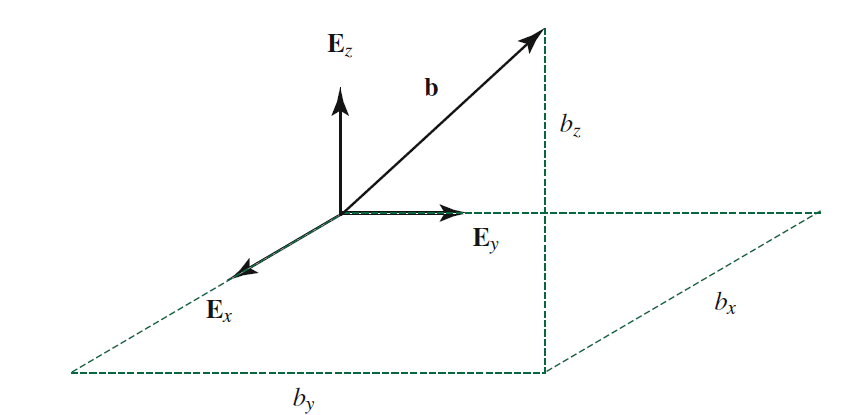
\includegraphics[width=0.5\linewidth,height=\textheight,keepaspectratio]{preliminaries/../figures/vector_calculus/cartesian_projection.PNG}

\begin{tcolorbox}[enhanced jigsaw, arc=.35mm, bottomrule=.15mm, bottomtitle=1mm, breakable, colback=white, colbacktitle=quarto-callout-tip-color!10!white, colframe=quarto-callout-tip-color-frame, coltitle=black, left=2mm, leftrule=.75mm, opacityback=0, opacitybacktitle=0.6, rightrule=.15mm, title=\textcolor{quarto-callout-tip-color}{\faLightbulb}\hspace{0.5em}{Think!}, titlerule=0mm, toprule=.15mm, toptitle=1mm]

Question: Calculate \({\bf E}_x \times {\bf E}_x\),
\({\bf E}_x \times {\bf E}_y\), etc.

\begin{quote}
\textbf{Answer}

\ldots{}
\end{quote}

\end{tcolorbox}

\begin{tcolorbox}[enhanced jigsaw, arc=.35mm, bottomrule=.15mm, bottomtitle=1mm, breakable, colback=white, colbacktitle=quarto-callout-tip-color!10!white, colframe=quarto-callout-tip-color-frame, coltitle=black, left=2mm, leftrule=.75mm, opacityback=0, opacitybacktitle=0.6, rightrule=.15mm, title=\textcolor{quarto-callout-tip-color}{\faLightbulb}\hspace{0.5em}{Think!}, titlerule=0mm, toprule=.15mm, toptitle=1mm]

Question: Calculate \({\bf E}_x \cdot {\bf E}_x\),
\({\bf E}_x \cdot {\bf E}_y\), etc.

\begin{quote}
\textbf{Answer}

\ldots{}
\end{quote}

\end{tcolorbox}

We can represent any vector \({\bf b}\) as

\begin{align}
    {\bf a} &= a_x {\bf E}_x + a_y {\bf E}_y + a_z {\bf E}_z,\\
    {\bf b} &= b_x {\bf E}_x + b_y {\bf E}_y + b_z {\bf E}_z.
\end{align}

We can write the scalar product and cross product of these vectors in
terms of their Cartesian components.

\begin{align}
    {\bf a} \cdot {\bf b} &= (a_x {\bf E}_x + a_y {\bf E}_y + a_z {\bf E}_z)\cdot(b_x {\bf E}_x + b_y {\bf E}_y + b_z {\bf E}_z)\\
    &= a_x b_x + a_y b_y + a_z b_z\\
    {\bf a} \times {\bf b} &= (a_x {\bf E}_x + a_y {\bf E}_y + a_z {\bf E}_z)\times (b_x {\bf E}_x + b_y {\bf E}_y + b_z {\bf E}_z)\\
    &= (a_y b_z - a_z b_y){\bf E}_x + (a_z b_x - a_x b_z){\bf E}_y + (a_x b_y - a_y b_x){\bf E}_z
\end{align}

\section{Differentiation of Vectors}\label{differentiation-of-vectors}

\begin{align}
    \frac{d{\bf u}}{dt} &= \frac{du_x}{dt}{\bf E}_x + \frac{du_y}{dt}{\bf E}_y + \frac{du_z}{dt}{\bf E}_z + u_x\frac{d{\bf E}_x}{dt} + u_y\frac{d{\bf E}_y}{dt} + u_z\frac{d{\bf E}_z}{dt}\\
    &= \frac{du_x}{dt}{\bf E}_x + \frac{du_y}{dt}{\bf E}_y + \frac{du_z}{dt}{\bf E}_z
\end{align}

\begin{align}
    \frac{d}{dt}({\bf u}\cdot{\bf v}) = \frac{d{\bf u}}{dt}\cdot{\bf v} + {\bf u}\cdot\frac{d{\bf v}}{dt}
\end{align}

\begin{align}
    \frac{d}{dt}({\bf u}\times{\bf v}) = \frac{d{\bf u}}{dt}\times{\bf v} + {\bf u}\times\frac{d{\bf v}}{dt}
\end{align}

\section{Sine Law and Cosine Law}\label{sine-law-and-cosine-law}

\begin{center}
\pandocbounded{
\includegraphics[keepaspectratio]{preliminaries/vector_calculus_files/figure-pdf/unnamed-chunk-6-1.pdf}}
\end{center}

Referring to the above triangle with interior angles \(A\), \(B\), and
\(C\) and with side lengths \(a\), \(b\), and \(c\), the sine law and
cosine law are respectively

\begin{align}
    \frac{\sin(A)}{a} &= \frac{\sin(B)}{b} = \frac{\sin(C)}{c},\\
    c^2 &= a^2 + b^2 - 2ab\cos(C).
\end{align}

\section{Exercises}\label{exercises-2}

\emph{The following problems are from Set 01 -- Vector Calculus.}

\textbf{1.} Two chords are pulling on a hook with tensions \(T_1 = 100\)
N and \(T_2 = 50\) N as shown. Using the parallelogram rule, determine
the magnitude of the resultant force and the angle it makes with the
horizontal. Do not introduce a Cartesian basis.

\begin{center}
\pandocbounded{
\includegraphics[keepaspectratio]{preliminaries/vector_calculus_files/figure-pdf/unnamed-chunk-7-1.pdf}}
\end{center}

\textbf{2.} Resolve the horizontal force \(F\) into components along the
\(u\) and \(v\) axes and determine the magnitudes of the components.

\begin{center}
\pandocbounded{
\includegraphics[keepaspectratio]{preliminaries/vector_calculus_files/figure-pdf/unnamed-chunk-8-1.pdf}}
\end{center}

\textbf{3.} In Exercise 1, take unit vectors \(\mathbf{I}\) and
\(\mathbf{J}\) to point horizontally leftwards and vertically upwards.
The unit vector \(\mathbf{K}\) completes the right-handed triad. Repeat
Exercise 1 by resolving all forces in the Cartesian
\(\{\mathbf{I},\mathbf{J},\mathbf{K}\}\) basis.

\textbf{4.} A particle moves in space with velocity \begin{align}
    \mathbf{v}(t) = 2t^2\mathbf{E}_1 - \mathbf{E}_2 + (-5t+3)\mathbf{E}_3 \quad \text{m/s}.
\end{align} (a) Calculate \(\mathbf{v}\) at \(t=1\) s. (b) Calculate
\(\mathbf{a}(t)\equiv\dot{\mathbf{v}}(t)\). (c) Given
\(\mathbf{r}(0)=2\mathbf{E}_3\), find \(\mathbf{r}(t)\).

\textbf{5.} A child at \(B\) pulls a chord attached to the wall at \(A\)
with a force of \(70\) N.

\begin{center}
\pandocbounded{
\includegraphics[keepaspectratio]{preliminaries/vector_calculus_files/figure-pdf/unnamed-chunk-9-1.pdf}}
\end{center}

\begin{enumerate}
\def\labelenumi{(\alph{enumi})}
\tightlist
\item
  Express the position vector \(\mathbf{r}_A\) in Cartesian coordinates.
\item
  Express the position vector \(\mathbf{r}_B\) in Cartesian coordinates.
\item
  Draw \(\mathbf{r}_{B/A} = \mathbf{r}_B - \mathbf{r}_A\). Does it point
  from \(B\) to \(A\) or from \(A\) to \(B\)?
\item
  Draw \(\mathbf{r}_{A/B}\).
\item
  What is the tension force \(\mathbf{T}\) in the cable?
\end{enumerate}

\textbf{6.} Referring to Exercises 1 and 3:

\begin{enumerate}
\def\labelenumi{(\alph{enumi})}
\tightlist
\item
  Calculate \(\mathbf{T}_1\times\mathbf{T}_2\) without using a basis.
\item
  Express \(\mathbf{T}_1\) and \(\mathbf{T}_2\) in the Cartesian basis
  from Exercise 3 and verify part (a).
\item
  What is \(\mathbf{T}_2\times\mathbf{T}_1\)?
\end{enumerate}

\chapter{Fundamental Concepts of Solid
Mechanics}\label{fundamental-concepts-of-solid-mechanics}

This section is adapted from chapter 1 of
\href{https://link.springer.com/book/10.1007/978-1-4614-6768-7}{Introduction
to Solid Mechanics - An Integrated Approach} by Lubliner and
Papadopoulos (Lubliner and Papadopoulos 2017).

\section{Mechanics}\label{mechanics}

Mechanics, as a scientific discipline, is the study of the behavior of
bodies subject to forces and displacements (and, to some extent, heating
and cooling).

\section{Solid Mechanics}\label{solid-mechanics}

Solid mechanics is the branch of mechanics dealing specifically with
solid bodies.

\section{Body}\label{body}

A body, for the purpose of mechanics, is a portion of matter that, at a
given moment in time, occupies a certain region in space.

\begin{itemize}
\tightlist
\item
  \textbf{Particle} If the region occupied by the body can be idealized
  as being of negligible extent (and thus reducible to a point), the
  body is called a particle.
\item
  \textbf{Finite Body} A body that is not reducible to a point is called
  a finite body.
\end{itemize}

\section{Continuum}\label{continuum}

A finite body occupying a connected region every portion of which
contains some matter is called a continuous body or, simply, a
continuum.

\section{Material Points}\label{material-points}

At any point in a region occupied by a continuum, the matter in its
immediate (infinitesimal) neighborhood can also be thought of as
constituting a particle, and we may thus speak of the particles (also
called material points) of a continuum.

\section{Displacement}\label{displacement}

A body is said to undergo a displacement when some or all of its
particles are moved to occupy different positions in space.

\section{Configuration}\label{configuration}

The correspondence between the particles and the positions occupied by
them at a given time is known as the body's configuration.

\section{Deformation}\label{deformation}

The displacement of a body is said to be rigid if the distances between
all pairs of particles are the same in any two configurations.
Otherwise, the body is said to undergo deformation.

\section{Rigid bodies}\label{rigid-bodies}

Bodies that can undergo only rigid displacements are called rigid
bodies. Bodies that are not rigid are deformable.

\section{Motion}\label{motion}

Motion is said to occur when the body occupies a succession of different
configurations continuously over time.

\section{Rigid Motion}\label{rigid-motion}

A rigid motion is a motion that involves only rigid displacements.

\section{Velocity}\label{velocity}

The rate of change, in time, of the position of a particle is its
velocity.

\section{Acceleration}\label{acceleration}

The velocity may in turn change in time, and its rate of change is the
acceleration. The motion of a body is called uniform if the acceleration
of all the particles is zero; otherwise, it is called accelerated.

\section{Kinematics}\label{kinematics}

The branch of mechanics dealing with the displacement and motion of
bodies is called kinematics.

\section{Force}\label{force}

Forces are interactions between bodies that cause them to move, and more
specifically to accelerate, relative to each other (unless prevented
from doing so by other forces).

\chapter{Galileo, Kepler, Newton}\label{galileo-kepler-newton}

\section{Gravitational force}\label{gravitational-force}

All bodies on or near the earth are subject to the earth's gravitational
force and, as shown by Galileo in his famous experiments, will fall
toward the center of the earth (unless prevented from doing so by other
forces) with the same acceleration; the magnitude of this acceleration
is denoted by \(g\).

It was later shown by Newton, on the basis of Kepler's laws of planetary
motion, that the magnitude of the acceleration (with respect to a frame
of reference based on the ``fixed'' stars) due to gravitational force
between any two bodies (idealized as particles) is inversely
proportional to the square of the distance between them, and for each
body it is proportional to the quantity of matter (or mass) of the other
body. The product of mass and acceleration is therefore equal and
opposite for the two bodies and may be identified with the force exerted
on each body by the other.

\url{https://youtu.be/icrTzMozNgo}

\section{Equilibrium}\label{equilibrium}

If a body's acceleration is zero, then it is at rest or in a uniform
motion. In this case, the forces is said to be in equilibrium. The study
of equilibrium is known as statics and constitutes one of the main
subjects of this book. Traditionally, statics deals only (or at least
primarily) with rigid bodies, while deformable bodies are studied in
courses historically called strength of materials (or, more recently,
mechanics of materials). In this book (Lubliner and Papadopoulos 2017),
the statics of rigid and deformable solid bodies will be studied in an
integrated manner.

\chapter{A Continuum Mechanics
Perspective}\label{a-continuum-mechanics-perspective}

Consider a body \(\mathcal{B}\) in three-dimensional Euclidean space
\(\mathbb{E}^3\).

\begin{center}
\pandocbounded{
\includegraphics[keepaspectratio]{preliminaries/continuum_mechanics_perspective_files/figure-pdf/unnamed-chunk-1-1.pdf}}
\end{center}

In general, bodies are deformable continua. We depict continua as in the
above figure and refer to them as \emph{continuum potatoes}.

Point or distributed forces or moments can be applied to a body's
surface or throughout its volume. For example, a body resting on a table
has contact forces on the surface touching the table, while weight acts
on all points in the body.

\begin{tcolorbox}[enhanced jigsaw, arc=.35mm, bottomrule=.15mm, bottomtitle=1mm, breakable, colback=white, colbacktitle=quarto-callout-tip-color!10!white, colframe=quarto-callout-tip-color-frame, coltitle=black, left=2mm, leftrule=.75mm, opacityback=0, opacitybacktitle=0.6, rightrule=.15mm, title=\textcolor{quarto-callout-tip-color}{\faLightbulb}\hspace{0.5em}{Think!}, titlerule=0mm, toprule=.15mm, toptitle=1mm]

\textbf{Question:} How do we know if a body has moved or deformed?

\begin{quote}
\textbf{Answer}

\ldots{}
\end{quote}

\end{tcolorbox}

Consider a reference configuration for this body. A reference
configuration is any configuration that can be physically occupied by
the body --- it could be the initial configuration, but need not be.

\begin{center}
\pandocbounded{
\includegraphics[keepaspectratio]{preliminaries/continuum_mechanics_perspective_files/figure-pdf/unnamed-chunk-2-1.pdf}}
\end{center}

We denote the position vector from a chosen fixed origin to a material
point in the reference configuration as \({\bf R}\). The position vector
to the same material point in the current configuration is \({\bf r}\).

The motion of the body is described by \begin{align}
    {\bf r} = \bchi({\bf R},t).
\end{align}

\begin{tcolorbox}[enhanced jigsaw, arc=.35mm, bottomrule=.15mm, bottomtitle=1mm, breakable, colback=white, colbacktitle=quarto-callout-tip-color!10!white, colframe=quarto-callout-tip-color-frame, coltitle=black, left=2mm, leftrule=.75mm, opacityback=0, opacitybacktitle=0.6, rightrule=.15mm, title=\textcolor{quarto-callout-tip-color}{\faLightbulb}\hspace{0.5em}{Think!}, titlerule=0mm, toprule=.15mm, toptitle=1mm]

\textbf{Question:} What makes a body rigid?

\begin{quote}
\textbf{Answer}

In this class, we consider only rigid bodies. If we choose two points on
a rigid body, the distance between them is always constant. Also, angles
between material lines on a rigid body are constant.
\end{quote}

\end{tcolorbox}

\begin{tcolorbox}[enhanced jigsaw, arc=.35mm, bottomrule=.15mm, bottomtitle=1mm, breakable, colback=white, colbacktitle=quarto-callout-tip-color!10!white, colframe=quarto-callout-tip-color-frame, coltitle=black, left=2mm, leftrule=.75mm, opacityback=0, opacitybacktitle=0.6, rightrule=.15mm, title=\textcolor{quarto-callout-tip-color}{\faLightbulb}\hspace{0.5em}{Think!}, titlerule=0mm, toprule=.15mm, toptitle=1mm]

\textbf{Question:} Under what conditions do we consider a rigid body to
be a particle?

\begin{quote}
\textbf{Answer}

In the beginning of the class, we consider particles. Particles are
idealized rigid bodies whose rotational inertia is ignored.
\end{quote}

\end{tcolorbox}

\part{Particle Dynamics}

\chapter{Particle Kinematics}\label{particle-kinematics}

\section{Position, Velocity, and
Acceleration}\label{position-velocity-and-acceleration}

Consider a particle moving in \(\mathbb{E}^3\). Its position vector
relative to a fixed origin \(O\) is denoted by
\({\bf r} \in \mathbb{E}^3\). As time \(t\) evolves, so does
\({\bf r}(t)\).

\begin{center}
\pandocbounded{
\includegraphics[keepaspectratio]{particle_dynamics/basic_particle_kinematics_files/figure-pdf/unnamed-chunk-1-1.pdf}}
\end{center}

Let \(\Delta t\) be a finite time elapsed: \begin{align}
    \Delta{\bf r} = {\bf r}(t+\Delta t)-{\bf r}(t).
\end{align} As \(\Delta t \rightarrow 0\), \(\Delta t\) becomes \(dt\)
and \(\Delta {\bf r}\) becomes \(d{\bf r}\). The `\(d\)' means
differential. We denote the time derivative of \({\bf r}\) by
\(\dot{\bf r}\) or \(\frac{d{\bf r}}{dt}\).

\begin{center}
\pandocbounded{
\includegraphics[keepaspectratio]{particle_dynamics/basic_particle_kinematics_files/figure-pdf/unnamed-chunk-2-1.pdf}}
\end{center}

The (absolute) velocity vector \({\bf v}\) of the particle is the time
rate of change of the position vector: \begin{align}
    {\bf v} = \frac{d{\bf r}}{dt}=\dot{\bf r} = \lim_{\Delta t \rightarrow 0}\frac{{\bf r}(t+\Delta t)-{\bf r}(t)}{\Delta t}.
\end{align}

\begin{tcolorbox}[enhanced jigsaw, arc=.35mm, bottomrule=.15mm, bottomtitle=1mm, breakable, colback=white, colbacktitle=quarto-callout-tip-color!10!white, colframe=quarto-callout-tip-color-frame, coltitle=black, left=2mm, leftrule=.75mm, opacityback=0, opacitybacktitle=0.6, rightrule=.15mm, title=\textcolor{quarto-callout-tip-color}{\faLightbulb}\hspace{0.5em}{Think!}, titlerule=0mm, toprule=.15mm, toptitle=1mm]

\textbf{Question:} What is the direction of the velocity vector?

\begin{quote}
\textbf{Answer}

\({\bf v}\) is along \(d{\bf r}\) which is always tangent to the path.
\end{quote}

\end{tcolorbox}

The speed of the particle is the magnitude of the velocity vector
\(v = \lnorm{\bf v}\rnorm\).

The (absolute) acceleration is \begin{align}
    {\bf a} = \frac{d{\bf v}}{dt} = \dot{\bf v} = \ddot{\bf r} = \frac{d^2{\bf r}}{dt^2}.
\end{align}

\section{Arc-Length and the Unit Tangent
Vector}\label{arc-length-and-the-unit-tangent-vector}

Define the arc-length parameter \(s\) such that \begin{align}
    \frac{ds}{dt} = \lnorm {\bf v}\rnorm.
\end{align}

\(\frac{ds}{dt}\) is the speed of the particle. Recall that
\({\bf v} = \frac{d{\bf r}}{dt}\), so \begin{align}
    \frac{ds}{dt} = \lnorm\frac{d{\bf r}}{dt}\rnorm.
\end{align}

So \(ds\) is the length of the differential \(d{\bf r}\) along the
curve. Integrating: \begin{align}
    s(t)-s_0 = \int_{t_0}^t\frac{ds}{dt}(\tau)d\tau = \int_{t_0}^t\sqrt{{\bf v}(\tau)\cdot{\bf v}(\tau)}\,d\tau.
\end{align}

Notes:

\begin{itemize}
\tightlist
\item
  \(s(t)-s_0\) is the distance traveled by the particle along its path
  \(\mathcal{C}\) during the time interval \([t_0, t]\).
\item
  \(s(t_0)=s_0\) where \(t_0\) and \(s_0\) are initial conditions.
\item
  The dummy variable \(\tau\) is used (as opposed to \(t\)) when
  evaluating this integral because we are integrating the speed as it
  varies between \(t_0\) and \(t\). The variable of integration is
  different than the upper limit of integration.
\end{itemize}

\begin{tcolorbox}[enhanced jigsaw, arc=.35mm, bottomrule=.15mm, bottomtitle=1mm, breakable, colback=white, colbacktitle=quarto-callout-tip-color!10!white, colframe=quarto-callout-tip-color-frame, coltitle=black, left=2mm, leftrule=.75mm, opacityback=0, opacitybacktitle=0.6, rightrule=.15mm, title=\textcolor{quarto-callout-tip-color}{\faLightbulb}\hspace{0.5em}{Think!}, titlerule=0mm, toprule=.15mm, toptitle=1mm]

\textbf{Question:} Under what conditions is \(s(t)\) invertible so that
\(t(s)\) is well defined?

\begin{quote}
\textbf{Answer}

If the function \(s(t)\) is one-to-one, it can be inverted, and time can
be written in terms of arc-length \(t = t(s)\).
\end{quote}

\end{tcolorbox}

\begin{tcolorbox}[enhanced jigsaw, arc=.35mm, bottomrule=.15mm, bottomtitle=1mm, breakable, colback=white, colbacktitle=quarto-callout-tip-color!10!white, colframe=quarto-callout-tip-color-frame, coltitle=black, left=2mm, leftrule=.75mm, opacityback=0, opacitybacktitle=0.6, rightrule=.15mm, title=\textcolor{quarto-callout-tip-color}{\faLightbulb}\hspace{0.5em}{Think!}, titlerule=0mm, toprule=.15mm, toptitle=1mm]

\textbf{Question:} Why is \begin{align}
    s(t)-s_0 \neq \lnorm {\bf r}(t)-{\bf r}_0\rnorm?
\end{align} Under what conditions does the equality hold?

\begin{quote}
\textbf{Answer}

The equality holds under rectilinear motion or over an infinitesimal
time interval.
\end{quote}

\end{tcolorbox}

We define the unit tangent vector \({\bf e}_t\): \begin{align}
    \frac{\bf v}{\lnorm{\bf v}\rnorm} = {\bf e}_t, \qquad {\bf v} = \frac{d{\bf r}}{dt} = \frac{d{\bf r}}{ds}\frac{ds}{dt} = \dot{s}{\bf e}_t.
\end{align}

\begin{tcolorbox}[enhanced jigsaw, arc=.35mm, bottomrule=.15mm, bottomtitle=1mm, breakable, colback=white, colbacktitle=quarto-callout-tip-color!10!white, colframe=quarto-callout-tip-color-frame, coltitle=black, left=2mm, leftrule=.75mm, opacityback=0, opacitybacktitle=0.6, rightrule=.15mm, title=\textcolor{quarto-callout-tip-color}{\faLightbulb}\hspace{0.5em}{Think!}, titlerule=0mm, toprule=.15mm, toptitle=1mm]

\textbf{Question:} Verify that \({\bf e}_t\) is a unit vector.

\begin{quote}
\textbf{Answer}

\ldots{}
\end{quote}

\end{tcolorbox}

Note the relationships \begin{align*}
    {\bf v} &= \frac{d{\bf r}(t)}{dt} = \frac{d{\bf r}}{ds}\frac{ds}{dt},\\
    {\bf a} &= \frac{d{\bf v}(t)}{dt} = \frac{d^2{\bf r}}{ds^2}\lp\frac{ds}{dt}\rp^2+\frac{d{\bf r}}{ds}\frac{d^2 s}{dt^2}.
\end{align*}

Notice: the acceleration vector is due to changes in both the magnitude
and direction of the velocity vector.

\begin{tcolorbox}[enhanced jigsaw, arc=.35mm, bottomrule=.15mm, bottomtitle=1mm, breakable, colback=white, colbacktitle=quarto-callout-tip-color!10!white, colframe=quarto-callout-tip-color-frame, coltitle=black, left=2mm, leftrule=.75mm, opacityback=0, opacitybacktitle=0.6, rightrule=.15mm, title=\textcolor{quarto-callout-tip-color}{\faLightbulb}\hspace{0.5em}{Think!}, titlerule=0mm, toprule=.15mm, toptitle=1mm]

\textbf{Question:} Is the unit vector \({\bf e}_t\) constant in general?
Under what conditions is it constant?

\begin{quote}
\textbf{Answer}

No.~It is constant only during rectilinear motion in a fixed direction.
\end{quote}

\end{tcolorbox}

\subsection{Example}\label{example}

\begin{tcolorbox}[enhanced jigsaw, arc=.35mm, bottomrule=.15mm, bottomtitle=1mm, breakable, colback=white, colbacktitle=quarto-callout-warning-color!10!white, colframe=quarto-callout-warning-color-frame, coltitle=black, left=2mm, leftrule=.75mm, opacityback=0, opacitybacktitle=0.6, rightrule=.15mm, title=\textcolor{quarto-callout-warning-color}{\faExclamationTriangle}\hspace{0.5em}{Example}, titlerule=0mm, toprule=.15mm, toptitle=1mm]

\textbf{Question:} Consider a particle moving in space with position
vector \begin{align}
    {\bf r}(t) = R_0\lp\cos(\omega t){\bf E}_x+\sin(\omega t){\bf E}_y\rp.
\end{align}

Calculate \({\bf v}\), \({\bf a}\), \({\bf v}\times {\bf a}\),
\(\lnorm{\bf r}\rnorm\). Describe the motion of the particle. Show that
the motion satisfies: \begin{align}
    \ddot{x}+\omega^2 x=0, \qquad \ddot{y}+\omega^2 y=0.
\end{align}

\begin{quote}
\textbf{Answer}

We calculate the velocity and acceleration vectors of the particle as
follows:

\begin{align*}
{\bf v} &= \frac{d{\bf r}}{dt}
= R_0\omega\left(-\sin(\omega t)\,{\bf E}_x+\cos(\omega t)\,{\bf E}_y\right),\\
{\bf a} &= \frac{d{\bf v}}{dt}
= -R_0\omega^2\left(\cos(\omega t)\,{\bf E}_x+\sin(\omega t)\,{\bf E}_y\right).
\end{align*}

As you take these derivatives, remember that:

\begin{itemize}
\tightlist
\item
  \(\dot{\bf E}_x={\bf 0}\) and \(\dot{\bf E}_y={\bf 0}\) since the
  basis \(\{{\bf E}_x,{\bf E}_y\}\) is fixed.
\item
  The chain rule: \(\frac{d}{dx}f(g(x)) = f'(g(x))g'(x).\)
\end{itemize}

Then,

\begin{align*}
{\bf r}\times{\bf a}
&=
R_0\left(\cos(\omega t){\bf E}_x+\sin(\omega t){\bf E}_y\right)
\times
\left(
-R_0\omega^2\left(\cos(\omega t){\bf E}_x+\sin(\omega t){\bf E}_y\right)
\right) \\
&=
-R_0^2\omega^2
\Big(
\cos^2(\omega t)\underbrace{{\bf E}_x\times{\bf E}_x}_{{\bf 0}}
+\cos(\omega t)\sin(\omega t)
\left(
\underbrace{{\bf E}_x\times{\bf E}_y}_{{\bf E}_z}
+
\underbrace{{\bf E}_y\times{\bf E}_x}_{-{\bf E}_z}
\right) \\
&\qquad\qquad
+\sin^2(\omega t)\underbrace{{\bf E}_y\times{\bf E}_y}_{{\bf 0}}
\Big) \\
&= {\bf 0}.
\end{align*}

Alternatively, notice that

\begin{align*}
{\bf a} = -\omega^2{\bf r},
\end{align*}

so

\begin{align*}
{\bf r}\times{\bf a}
=
{\bf r}\times(-\omega^2{\bf r})
=
-\omega^2({\bf r}\times{\bf r})
=
{\bf 0}.
\end{align*}

For practice, let us also calculate \({\bf r}\cdot{\bf a}\):

\begin{align*}
{\bf r}\cdot{\bf a}
&=
R_0\left(\cos(\omega t){\bf E}_x+\sin(\omega t){\bf E}_y\right)
\cdot
\left(
-R_0\omega^2\left(\cos(\omega t){\bf E}_x+\sin(\omega t){\bf E}_y\right)
\right) \\
&=
-R_0^2\omega^2
\Big(
\cos^2(\omega t)\underbrace{{\bf E}_x\cdot{\bf E}_x}_{1}
+\cos(\omega t)\sin(\omega t)
\left(
\underbrace{{\bf E}_x\cdot{\bf E}_y}_{0}
+
\underbrace{{\bf E}_y\cdot{\bf E}_x}_{0}
\right)
+\sin^2(\omega t)\underbrace{{\bf E}_y\cdot{\bf E}_y}_{1}
\Big) \\
&=
-R_0^2\omega^2
\left(\cos^2(\omega t)+\sin^2(\omega t)\right) \\
&=
-R_0^2\omega^2.
\end{align*}

Alternatively,

\begin{align*}
{\bf r}\cdot{\bf a}
&=
{\bf r}\cdot(-\omega^2{\bf r}) \\
&=
-\omega^2({\bf r}\cdot{\bf r}) \\
&=
-\omega^2\|{\bf r}\|^2 \\
&=
-\omega^2R_0^2.
\end{align*}

Noting that \({\bf a} = -\omega^2{\bf r}\), we can show that the given
\({\bf r}\) satisfies the given differential equations: \begin{align*}
    {\bf r}\times{\bf a} = {\bf r}\times(-\omega^2{\bf r}) = -\omega^2{\bf r}\times{\bf r} = {\bf 0}.
\end{align*}

For \({\bf r}\cdot{\bf a}\): \begin{align*}
    {\bf r}\cdot{\bf a} &= -R_0^2\omega^2\lp\cos^2(\omega t)+\sin^2(\omega t)\rp = -R_0^2\omega^2.
\end{align*}
\end{quote}

\end{tcolorbox}

\section{Cartesian Coordinates}\label{cartesian-coordinates}

\(\{{\bf E}_x,{\bf E}_y,{\bf E}_z\}\) is a basis for \(\mathbb{E}^3\).
Since this basis is fixed, we have: \begin{align}
    {\bf r} &= x{\bf E}_x+y{\bf E}_y+z{\bf E}_z,\\
    {\bf v} &= \dot{x}{\bf E}_x+\dot{y}{\bf E}_y+\dot{z}{\bf E}_z,\\
    {\bf a} &= \ddot{x}{\bf E}_x+\ddot{y}{\bf E}_y+\ddot{z}{\bf E}_z.
\end{align}

Later we will also use the cylindrical polar basis
\(\{{\bf e}_r,{\bf e}_\theta,{\bf E}_z\}\) and the Serret-Frenet triad
\(\{{\bf e}_t,{\bf e}_n,{\bf e}_b\}\).

\section{Rectilinear Motion}\label{rectilinear-motion}

\begin{itemize}
\tightlist
\item
  \emph{rectus} = straight, \emph{linea} = line
\end{itemize}

Due to constraints or initial conditions, the body moves on a straight
line, e.g.~a car on a straight road or a ball tossed vertically.

We take \({\bf E}_x\) parallel to the line and \({\bf c}\) to be a
constant vector. Then: \begin{align}
    {\bf r}(t) &= x(t){\bf E}_x+{\bf c},\\
    {\bf v}(t) &= \dot{x}{\bf E}_x = v(t){\bf E}_x,\\
    {\bf a}(t) &= \ddot{x}{\bf E}_x = a(t){\bf E}_x.
\end{align}

\(\frac{ds}{dt}=\left|\frac{dx}{dt}\right|\), so unless \(\dot{x}>0\) or
\(\dot{x}<0\) throughout, \(x\) and \(s\) cannot be easily interchanged
as this convention flips \({\bf e}_t\) based on the motion.

\subsection{Identities for Rectilinear
Motion}\label{identities-for-rectilinear-motion}

Recall the definitions \({\bf v} = \frac{d{\bf r}}{dt}\) and
\({\bf a} = \frac{d{\bf v}}{dt}\). For the case of rectilinear motion
along \({\bf E}_x\), projecting these equations along \({\bf E}_x\)
yields respectively \(v = \frac{dx}{dt}\) and \(a = \frac{dv}{dt}\).
Applying the chain rule to the latter equation, we obtain \begin{align}
    a = \frac{dv}{dt} = \frac{dv}{dx}\frac{dx}{dt} = v\frac{dv}{dx}.
\end{align} where we assumed that \(v(t)\) can be written in terms of
\(x\).

We will now examine three useful identities for rectilinear motion that
relate \(s\), \(v\), and \(a\). \begin{align}
    ds &= v\, dt, \qquad dv = a\, dt, \qquad v\,dv = a\,ds.
\end{align}

\subsection{Given Acceleration as a Function of
Time}\label{given-acceleration-as-a-function-of-time}

From \(dv = a\, dt\), we can integrate this equation to get the signed
speed as a function of time. \begin{align}
    v(t)-v(t_0) = \int_{t_0}^{t}a(\tilde{t})\,d\tilde{t}.
\end{align} From \(ds = v\, dt\): \begin{align}
    s(t_1)-s(t_0) = \int_{s(t_0)}^{s(t_1)}d(\tilde{s}) =\int_{t_0}^{t_1}v(\tilde{t})\,d\tilde{t}.
\end{align} Note the use of the dummy variables \(\tilde{s}\) and
\(\tilde{t}\) in the above integrals.

\subsection{Given Acceleration as a Function of
Speed}\label{given-acceleration-as-a-function-of-speed}

Given \(a=a(v)\), we can use again \begin{align}
    dv = a dt
\end{align} to get \begin{align}
    \begin{split}
        dt &= \frac{dv}{a(v)}\\
        t(v) - t(v_0) &= \int_{v_0}^{v}\frac{d\tilde{v}}{a(\tilde{v})}
    \end{split} 
\end{align} Also, using the chain rule \begin{align}
\begin{split}
    a &= \frac{dv}{dt} = \frac{dv}{ds}\frac{ds}{dt}=v\frac{dv}{ds}\\
\end{split}
\end{align} If \(a=a(v)\), then \begin{align}
    \begin{split}
        ds &= \frac{vdv}{a}\\
        s(t)-s_0 &=\int_{v_0}^{v}\frac{\tilde{v}d\tilde{v}}{a(\Tilde{v})}.
    \end{split}
\end{align}

\subsection{Given Acceleration as a Function of
Displacement}\label{given-acceleration-as-a-function-of-displacement}

Starting with \(a = v\,dv/ds\), if \(a=a(s)\), we can rearrange this
equation to get \begin{align*}
\int_{v(s_0)}^{v(s)} v\,dv
=
\int_{s_0}^{s} a(\tilde{s})\,d\tilde{s}.
\end{align*}

Evaluating the left-hand side gives

\begin{align*}
\frac{1}{2}\left(v^2(s)-v^2(s_0)\right)
=
\int_{s_0}^{s} a(\tilde{s})\,d\tilde{s}.
\end{align*}

Equivalently,

\begin{align*}
v^2(s)
=
v^2(s_0)
+
2\int_{s_0}^{s} a(\tilde{s})\,d\tilde{s}.
\end{align*}

\subsection{Constant Acceleration}\label{constant-acceleration}

\subsubsection{Example: Gravity}\label{example-gravity}

Throw a ball upward and take your hand to be the origin.

Here,

\begin{align*}
{\bf a} = -g\,{\bf e}_t,
\qquad
g = 32.2\ \frac{\text{ft/s}}{\text{s}}.
\end{align*}

Note that \({\bf e}_t\) always points in the direction of increasing
\(s\) (upward). Therefore,

\begin{align*}
a=-g.
\end{align*}

Using

\begin{align*}
dv=a\,dt,
\end{align*}

we obtain

\begin{align*}
\int_{v(t_0)}^{v(t)} dv
&=
-g\int_{t_0}^{t} d\tilde{t},\\
v(t)-v(t_0)
&=
-g(t-t_0).
\end{align*}

Letting \(v(t_0)=v_0\) and choosing the time origin so that \(t_0=0\),
we find

\begin{align*}
v(t)=v_0-gt.
\end{align*}

To determine the position as a function of time, use

\begin{align*}
ds=v\,dt.
\end{align*}

Integrating,

\begin{align*}
\int_{s_0}^{s(t)} ds
&=
\int_{0}^{t}\left(v_0-g\tilde{t}\right)d\tilde{t},\\
s(t)-s_0
&=
v_0t-\frac{g}{2}t^2.
\end{align*}

Hence,

\begin{align*}
s(t)=s_0+v_0t-\frac{g}{2}t^2.
\end{align*}

In this example, \(s_0=0\).

\subsubsection{Example: Vehicle Braking}\label{example-vehicle-braking}

For constant acceleration, the relation

\begin{align*}
v\,dv=a\,ds
\end{align*}

is particularly useful.

Integrating,

\begin{align*}
\int_{v(s_0)}^{v(s)} v\,dv
&=
a\int_{s_0}^{s} d\tilde{s},\\
\frac{1}{2}\left(v^2(s)-v^2(s_0)\right)
&=
a(s-s_0).
\end{align*}

Therefore,

\begin{align*}
v^2(s)-v^2(s_0)
=
2a(s-s_0),
\end{align*}

or, in increment notation,

\begin{align*}
\Delta(v^2)=2a\,\Delta s.
\end{align*}

This equation is commonly used to determine braking distance when the
deceleration is approximately constant.

\section{Summary}\label{summary-1}

\textbf{Kinematics in Cartesian coordinates:} \begin{align}
    \mathbf{r} &= x\mathbf{E}_x + y\mathbf{E}_y + z\mathbf{E}_z, \\
    \mathbf{v} &= \dot{x}\mathbf{E}_x + \dot{y}\mathbf{E}_y + \dot{z}\mathbf{E}_z, \\
    \mathbf{a} &= \ddot{x}\mathbf{E}_x + \ddot{y}\mathbf{E}_y + \ddot{z}\mathbf{E}_z.
\end{align}

\textbf{Rectilinear motion} (along \(\mathbf{E}_x\)):
\(\mathbf{r}=x\mathbf{E}_x\), \(\mathbf{v}=\dot{x}\mathbf{E}_x\),
\(\mathbf{a}=\ddot{x}\mathbf{E}_x\), and \(a = v\,dv/dx\).

\section{Exercises}\label{exercises-3}

\emph{The following problems are from Set 03 -- Rectilinear Motion.}

\textbf{1.} {[}MKB 2/24{]} Solve \(a(x)\) as a piecewise function.
\emph{(ans. \(v = 8\) ft/sec)}

\begin{figure}[H]

{\centering 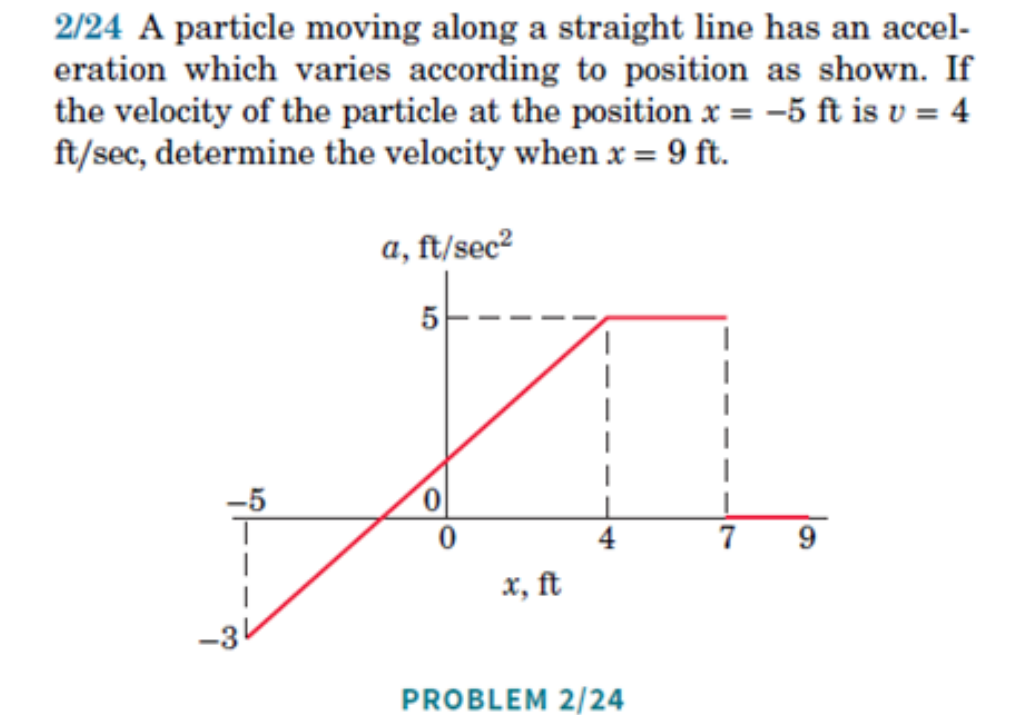
\includegraphics[width=0.5\linewidth,height=\textheight,keepaspectratio]{particle_dynamics/../figures/basic_particle_kinematics/02-024.jpg}

}

\caption{MKB 2/24.}

\end{figure}%

\textbf{2.} {[}MKB 2/28{]} Take \(\mathbf{E}_x\) along the horizontal;
origin at the location of the plane when the parachute deploys
(\(v=200\) mi/hr). Convert mi to ft and hr to sec.~\emph{(ans.
\(s = 5810\) ft)}

\begin{figure}[H]

{\centering 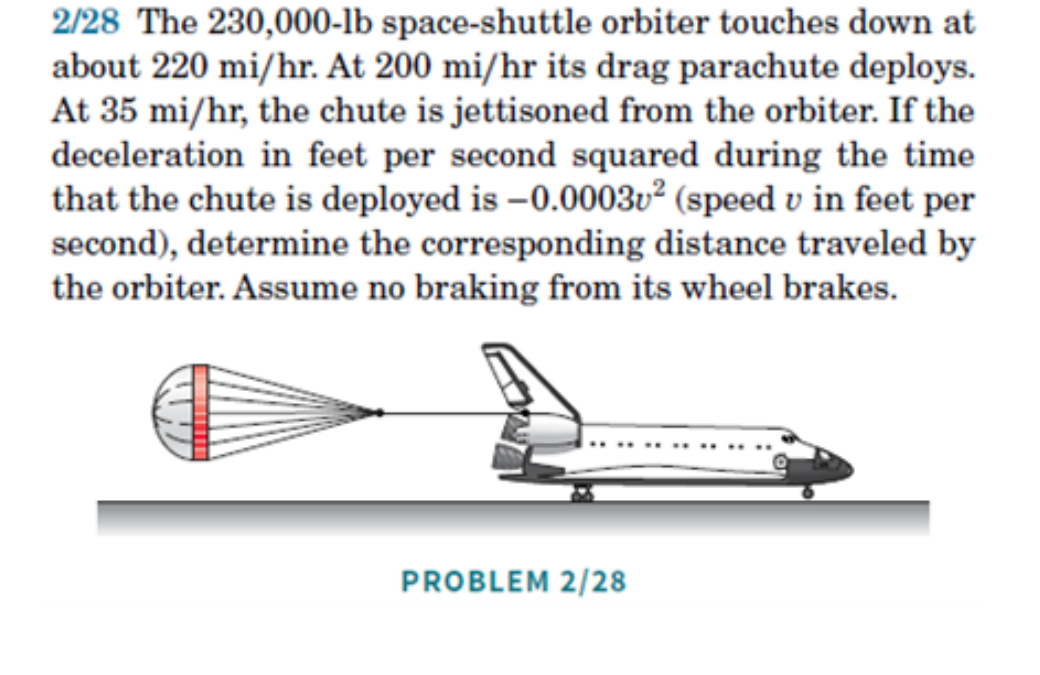
\includegraphics[width=0.5\linewidth,height=\textheight,keepaspectratio]{particle_dynamics/../figures/basic_particle_kinematics/02-028.jpg}

}

\caption{MKB 2/28.}

\end{figure}%

\textbf{3.} {[}MKB 2/25{]} Take \(\mathbf{E}_y\) vertically upwards;
origin at the initial position of the rocket. The acceleration is
\begin{align}
    a = \begin{cases} 3 \text{ m/s}^2 & 0\le t < 8\,\text{s} \\ -9.81 \text{ m/s}^2 & 8\,\text{s}\le t < t_{\mathrm{top}} \\ 0 & t_{\mathrm{top}} < t \le t_{\mathrm{end}} \end{cases}
\end{align} \emph{(ans. \(h = 125.4\) m, total time \(= 157.9\) s)}

\begin{figure}[H]

{\centering 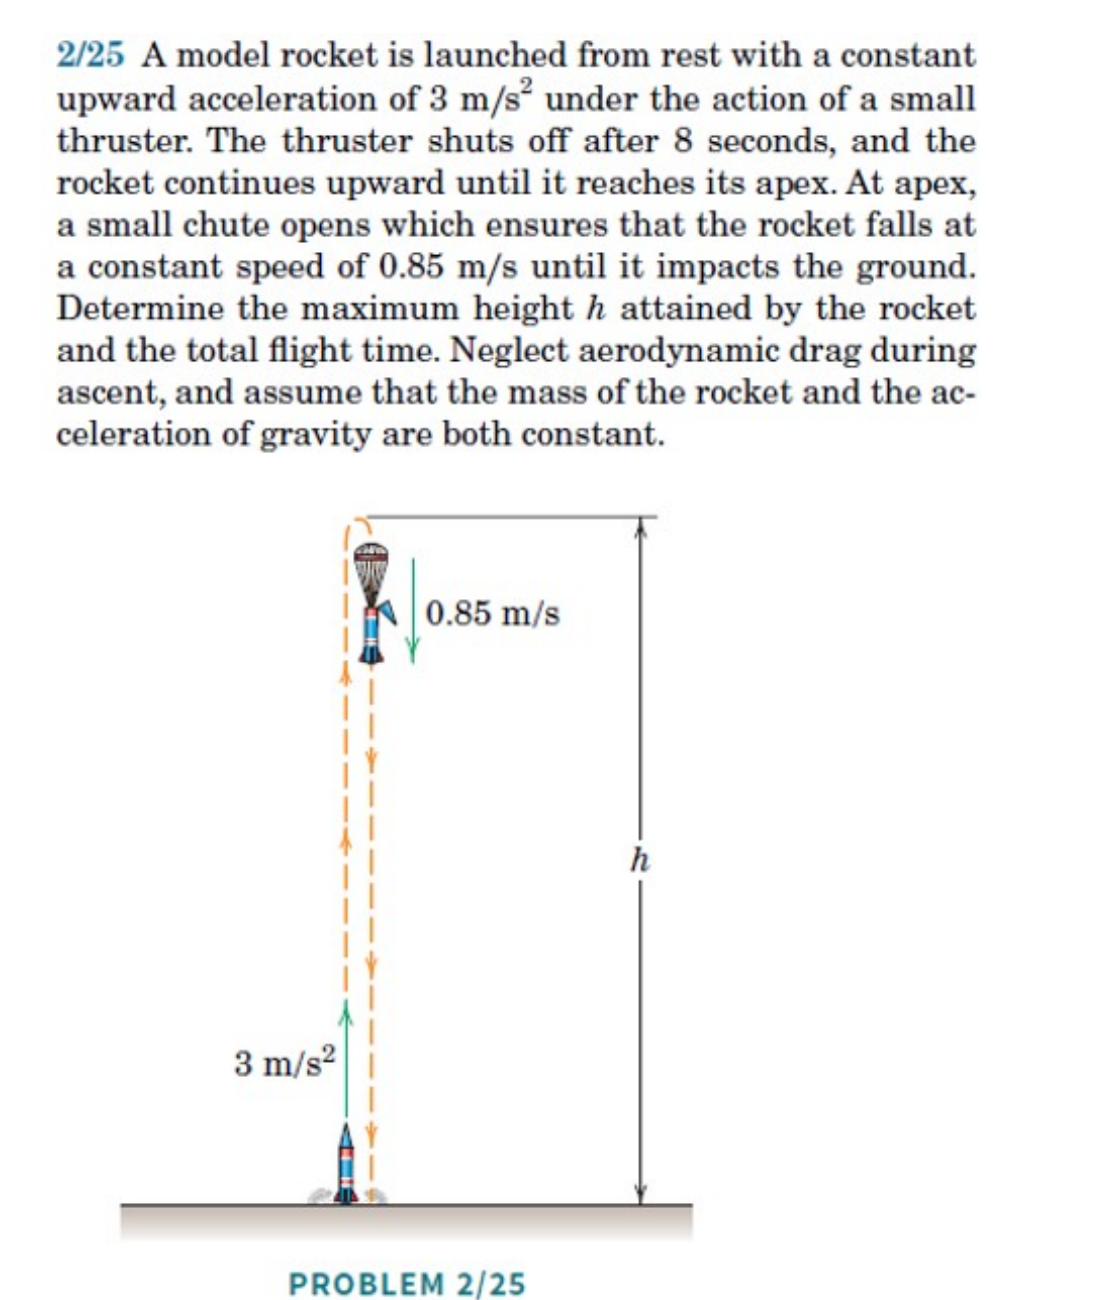
\includegraphics[width=0.5\linewidth,height=\textheight,keepaspectratio]{particle_dynamics/../figures/basic_particle_kinematics/02-025.jpg}

}

\caption{MKB 2/25.}

\end{figure}%

\textbf{4.} {[}MKB 2/22{]}

\begin{figure}[H]

{\centering 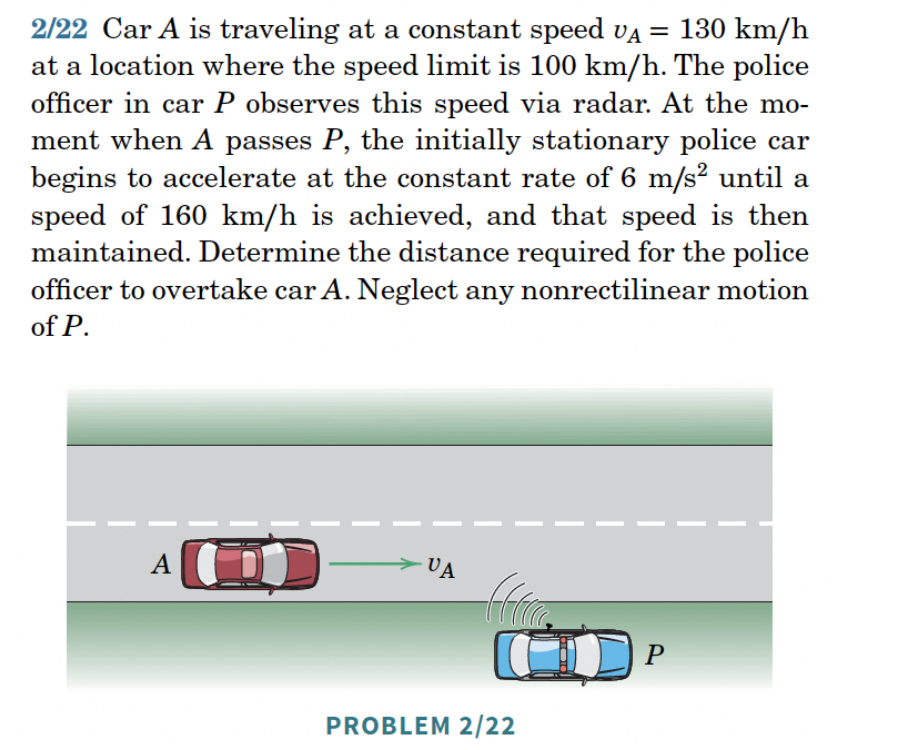
\includegraphics[width=0.5\linewidth,height=\textheight,keepaspectratio]{particle_dynamics/../figures/basic_particle_kinematics/02-022.jpg}

}

\caption{MKB 2/22.}

\end{figure}%

\chapter{Particle Kinetics}\label{particle-kinetics}

\section{The Balance of Linear
Momentum}\label{the-balance-of-linear-momentum}

A particle is endowed with an inertial measure \(m\), called its mass.

The linear momentum of a particle is defined to be \begin{align}
    {\bf G} = m{\bf v}.
\end{align} Taking the time derivative: \begin{align}
    \dot{\bf G} = \dot{m}{\bf v}+m\dot{\bf v}.
\end{align}

\begin{tcolorbox}[enhanced jigsaw, arc=.35mm, bottomrule=.15mm, bottomtitle=1mm, breakable, colback=white, colbacktitle=quarto-callout-tip-color!10!white, colframe=quarto-callout-tip-color-frame, coltitle=black, left=2mm, leftrule=.75mm, opacityback=0, opacitybacktitle=0.6, rightrule=.15mm, title=\textcolor{quarto-callout-tip-color}{\faLightbulb}\hspace{0.5em}{Think!}, titlerule=0mm, toprule=.15mm, toptitle=1mm]

\textbf{Question:} Can you think of systems whose mass is not conserved?

\begin{quote}
\textbf{Answer}

In this class, we consider cases where mass is conserved,
i.e.~\(\dot{m} = 0\). This is not the case, for example, for a launching
rocket that is losing mass. The \(\dot{m}{\bf v}\) term is useful in
control volume analysis.
\end{quote}

\end{tcolorbox}

Then, in our case of interest: \begin{align}
    \dot{\bf G} = m\dot{\bf v} = m{\bf a}.
\end{align} We postulate the following balance law/axiom/postulate to be
true: \begin{align}
    {\bf F} = \dot{\bf G},
\end{align} where \({\bf F}\) is the resultant external force acting on
the particle. This is known as the \textbf{Balance of Linear Momentum},
\textbf{Newton's Second Law}, or \textbf{Euler's First Law}.

\textbf{Important:} \({\bf a}\) here is the absolute acceleration vector
of the particle.

\begin{tcolorbox}[enhanced jigsaw, arc=.35mm, bottomrule=.15mm, bottomtitle=1mm, breakable, colback=white, colbacktitle=quarto-callout-tip-color!10!white, colframe=quarto-callout-tip-color-frame, coltitle=black, left=2mm, leftrule=.75mm, opacityback=0, opacitybacktitle=0.6, rightrule=.15mm, title=\textcolor{quarto-callout-tip-color}{\faLightbulb}\hspace{0.5em}{Think!}, titlerule=0mm, toprule=.15mm, toptitle=1mm]

\textbf{Question:} Under what conditions is the linear momentum
\({\bf G}\) conserved?

\begin{quote}
\textbf{Answer}

An unbalanced net force \({\bf F}\neq {\bf 0}\) results in a change of
\({\bf G}\). If \({\bf F}={\bf 0}\), then \({\bf G}={\bf c}\) where
\({\bf c}\) is a constant vector. This is Newton's First Law.
\end{quote}

\end{tcolorbox}

If \({\bf c}={\bf 0}\), we recover statics.

\subsection{Representations and
Projections}\label{representations-and-projections}

Vectors are represented on a basis. For example: \begin{align}
    {\bf F} &= F_x{\bf E}_x+F_y{\bf E}_y+ F_z{\bf E}_z,\\
    {\bf a} &= a_x{\bf E}_x+a_y{\bf E}_y+a_z{\bf E}_z.
\end{align}

\begin{tcolorbox}[enhanced jigsaw, arc=.35mm, bottomrule=.15mm, bottomtitle=1mm, breakable, colback=white, colbacktitle=quarto-callout-tip-color!10!white, colframe=quarto-callout-tip-color-frame, coltitle=black, left=2mm, leftrule=.75mm, opacityback=0, opacitybacktitle=0.6, rightrule=.15mm, title=\textcolor{quarto-callout-tip-color}{\faLightbulb}\hspace{0.5em}{Think!}, titlerule=0mm, toprule=.15mm, toptitle=1mm]

\textbf{Question:} How many independent scalar equations can we obtain
from \({\bf F}=m{\bf a}\)? How do we obtain them?

\begin{quote}
\textbf{Answer}

We get useful scalar equations by projecting \({\bf F} = \dot{\bf G}\)
along unit directions: \begin{align}
    \lp{\bf F}=\dot{\bf G}\rp\cdot{\bf E}_x \implies F_x = ma_x.
\end{align}
\end{quote}

\end{tcolorbox}

\section{Newton's Third Law}\label{newtons-third-law}

When dealing with the forces of interaction between particles, a
particle and a rigid body, or rigid bodies, we also invoke Newton's
third law: ``For every action there is an equal and opposite reaction.''
For example, the force exerted by a surface on a particle is equal in
magnitude and opposite in direction to the force exerted by the particle
on the surface.

\section{Four Steps to Problem Solving Using the
BoLM}\label{four-steps-to-problem-solving-using-the-bolm}

\begin{enumerate}
\def\labelenumi{\arabic{enumi}.}
\tightlist
\item
  Specify the system you are considering. Pick a frame (choose an origin
  and a coordinate system), and express \({\bf r}\), \({\bf v}\) and
  \({\bf a}\) using that coordinate system.
\item
  Draw a Free Body Diagram (FBD), i.e.~model of the forces.
\item
  Write the balance of linear momentum for the system:
  \({\bf F}=\dot{\bf G}\).
\item
  Do the analysis: project \({\bf F}=\dot{\bf G}\) to get useful
  equations.
\end{enumerate}

\subsection{Example: Projectile Motion}\label{example-projectile-motion}

Projectile motion is a curvilinear motion in the plane \(\mathbb{E}^2\).

\begin{center}
\pandocbounded{
\includegraphics[keepaspectratio]{particle_dynamics/particle_kinetics_files/figure-pdf/unnamed-chunk-1-1.pdf}}
\end{center}

\begin{enumerate}
\def\labelenumi{\arabic{enumi}.}
\item
  Choose \(O\) at the launch point, \({\bf E}_x\) along the ground,
  \({\bf E}_y\) against gravity. \begin{align}
   {\bf r} &= x{\bf E}_x+y{\bf E}_y, \quad {\bf v} = \dot{x}{\bf E}_x+\dot{y}{\bf E}_y, \quad {\bf a} = \ddot{x}{\bf E}_x+\ddot{y}{\bf E}_y.
  \end{align}
\item
  Force model:
\end{enumerate}

\begin{figure}[H]

{\centering 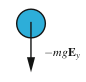
\includegraphics[width=0.1\linewidth,height=\textheight,keepaspectratio]{particle_dynamics/../figures/four_steps_bolm/FBD.png}

}

\caption{FBD}

\end{figure}%

\begin{align}
    {\bf W} = mg\lp-{\bf E}_y\rp.
\end{align}

\begin{enumerate}
\def\labelenumi{\arabic{enumi}.}
\setcounter{enumi}{2}
\item
  Balance of linear momentum: \begin{align}
   mg(-{\bf E}_y) = m\lp\ddot{x}{\bf E}_x+\ddot{y}{\bf E}_y\rp.
  \end{align} Projecting: \begin{align}
   \lp{\bf F}=\dot{\bf G}\rp\cdot{\bf E}_x &\implies 0 = m\ddot{x} \implies \ddot{x} = 0,\\
   \lp{\bf F}=\dot{\bf G}\rp\cdot{\bf E}_y &\implies -mg = m\ddot{y} \implies \ddot{y} = -g.
  \end{align}
\item
  Integrating: \begin{align}
   \dot{x}(t) &= \dot{x}_0, \quad x(t) = \dot{x}_0 t,\\
   \dot{y}(t) &= -gt+\dot{y}_0, \quad y(t) = -\frac{g}{2}t^2+\dot{y}_0 t+y_0.
  \end{align}
\end{enumerate}

\textbf{Remark:} You can also project \({\bf F} = m{\bf a}\) in the
\({\bf E}_z\) direction, but since there are no forces in that direction
and the initial velocity in that direction is 0, you conclude that the
motion is planar.

\subsection{Example: Projectile Motion with Viscous
Drag}\label{example-projectile-motion-with-viscous-drag}

\emph{(Primer Section 1.5.3)}

Going through the four steps, we get

\begin{enumerate}
\def\labelenumi{\arabic{enumi}.}
\tightlist
\item
  Again,
\end{enumerate}

\begin{align}
    {\bf r} &= x{\bf E}_x+y{\bf E}_y, \quad {\bf v} = \dot{x}{\bf E}_x+\dot{y}{\bf E}_y, \quad {\bf a} = \ddot{x}{\bf E}_x+\ddot{y}{\bf E}_y.
\end{align}

\begin{enumerate}
\def\labelenumi{\arabic{enumi}.}
\setcounter{enumi}{1}
\tightlist
\item
  Force model --- weight and Stokes drag:
\end{enumerate}

\begin{center}
\pandocbounded{
\includegraphics[keepaspectratio]{particle_dynamics/particle_kinetics_files/figure-pdf/unnamed-chunk-2-1.pdf}}
\end{center}

\begin{align}
    {\bf W} &= mg(-{\bf E}_y),\\
    {\bf F}_D &= \underbrace{c_s \lnorm{\bf v}\rnorm}_{\text{magnitude}}\underbrace{\lp-\frac{{\bf v}}{\lnorm{\bf v}\rnorm}\rp}_{\text{unit direction}} = -c_s{\bf v}.
\end{align} The Stokes drag (1851) applies at low speeds in viscous
fluids.

\begin{enumerate}
\def\labelenumi{\arabic{enumi}.}
\setcounter{enumi}{2}
\item
  Balance of linear momentum: \begin{align}
   {\bf F} &= \dot{\bf G},\\
   -mg{\bf E}_y -c_s\lp\dot{x}{\bf E}_x+\dot{y}{\bf E}_y\rp &= m\lp\ddot{x}{\bf E}_x+\ddot{y}{\bf E}_y\rp.
  \end{align} Projecting: \begin{align}
   \lp{\bf F}=\dot{\bf G}\rp\cdot{\bf E}_x &\implies\quad -c_s\dot{x} = m\ddot{x}\\
   \lp{\bf F}=\dot{\bf G}\rp\cdot{\bf E}_y &\implies\quad -mg-c_s\dot{y} = m\ddot{y}
  \end{align} Given initial conditions
  \(x_0, \dot{x}_0, y_0, \dot{y}_0\), these are an initial value problem
  (IVP).
\item
  Solving the \(x\)-equation (let \(v_x = \dot{x}\)): \begin{align}
       \lp{\bf F}=\dot{\bf G}\rp\cdot{\bf E}_x &\implies\quad -c_s\dot{x} = m\ddot{x},\\
       \lp{\bf F}=\dot{\bf G}\rp\cdot{\bf E}_y &\implies\quad -mg-c_s\dot{y} = m\ddot{y}.
  \end{align} These equations give ODEs for \(x(t)\) and \(y(t)\). Given
  IC's \(x_0, \dot{x}_0, y_0, \dot{y}_0\), we have an initial value
  problem (IVP).
\end{enumerate}

The \(x\)-equation is a first order ODE for \(v_x = \dot{x}\):
\begin{align}
    \begin{split}
        -c_s v_x &= m\Dot{v}_x\\
        -\frac{c_s}{m}dt &= \frac{d v_x}{v_x}\\
        -\frac{c_s}{m}\int_0^t d\Tilde{t} &= \int_{v_{x_0}}^{v_c(t)}\frac{d\Tilde{v}_x}{\tilde{v}_x}\\
        -\frac{c_s}{m}t &= \ln\lp\frac{v_x}{v_{x_0}}\rp\\
        v_x &= v_{x_0}e^{-\frac{c_s t}{m}}
    \end{split}
\end{align} Note that \begin{align}
    \lim_{t\rightarrow\infty} v_x = 0.
\end{align} Thus, the terminal velocity of the particle is only along
\({\bf E}_y\).

\begin{center}
\pandocbounded{
\includegraphics[keepaspectratio]{particle_dynamics/particle_kinetics_files/figure-pdf/unnamed-chunk-3-1.pdf}}
\end{center}

Solving the \(y\)-equation: \begin{align}
    dt &= \frac{m dv_y}{-mg-c_s v_y}\\
    \int_0^td\tilde{t} &= m\int_{v_{y_0}}^{v_y(t)}\frac{d\Tilde{v}_y}{-mg-c_s\Tilde{v}_y}\\
    v_y &= -\frac{mg}{c_s}+\frac{1}{c_s}\lp mg+c_s v_{y_0}\rp e^{-c_st/m}
\end{align} As \(t\rightarrow\infty\),
\(v_y \rightarrow -\frac{mg}{c_s}\). Thus, the terminal velocity
\begin{align}
    {\bf v}_{\text{term}} = \frac{mg}{c_s}\lp-{\bf E}_y\rp.
\end{align} \begin{align}
    v_y = -\frac{mg}{c_s}+\frac{1}{c_s}\lp mg+c_s v_{y_0}\rp e^{-c_s t/m}.
\end{align}

\subsection{Example: Projectile Motion with Bluff Body Pressure
Drag}\label{example-projectile-motion-with-bluff-body-pressure-drag}

\begin{figure}[H]

{\centering 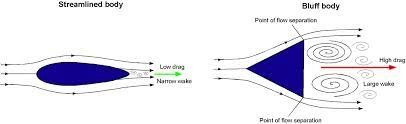
\includegraphics[width=0.5\linewidth,height=\textheight,keepaspectratio]{particle_dynamics/../figures/four_steps_bolm/bluff_body.jpeg}

}

\caption{Bluff body pressure drag}

\end{figure}%

\begin{align}
    {\bf F}_D = \frac{1}{2}m C_D v^2\lp-\frac{\bf v}{\lnorm{\bf v}\rnorm}\rp,
\end{align} where \(C_D\) is the drag coefficient, \(\rho\) is the
density of the fluid, and \(A\) is the projected area in the direction
of motion.

The equations of motion in this case (see primer section 1.6) need to be
solved numerically. One way to do this is described in the video below.

\url{https://youtu.be/RMkMK32vqyM}

\section{Summary}\label{summary-2}

\textbf{Balance of linear momentum (BoLM / Newton's 2nd law / Euler's
1st law):} \begin{align}
    \mathbf{F} = \dot{\mathbf{G}} = m\mathbf{a}.
\end{align}

\textbf{The four steps:}

\begin{enumerate}
\def\labelenumi{\arabic{enumi}.}
\tightlist
\item
  Choose an origin; draw basis vectors; write and differentiate the
  position vector \(\mathbf{r}\).
\item
  Draw the free body diagram; write expressions for all forces.
\item
  Write the vector BoLM equation \(\sum\mathbf{F} = m\mathbf{a}\).
\item
  Project along chosen directions and analyse to answer the question.
\end{enumerate}

\section{Exercises}\label{exercises-4}

\emph{The following problems are from Set 04 -- Balance of Linear
Momentum.}

\textbf{1.} {[}MKB 2/75{]} Take \(\mathbf{E}_x\) along the incline and
\(\mathbf{E}_y\) perpendicular to it (upwards); origin at \(A\). Follow
the 4 steps. \emph{(ans. \(\theta = (90^\circ + \alpha)/2\))}

\begin{figure}[H]

{\centering 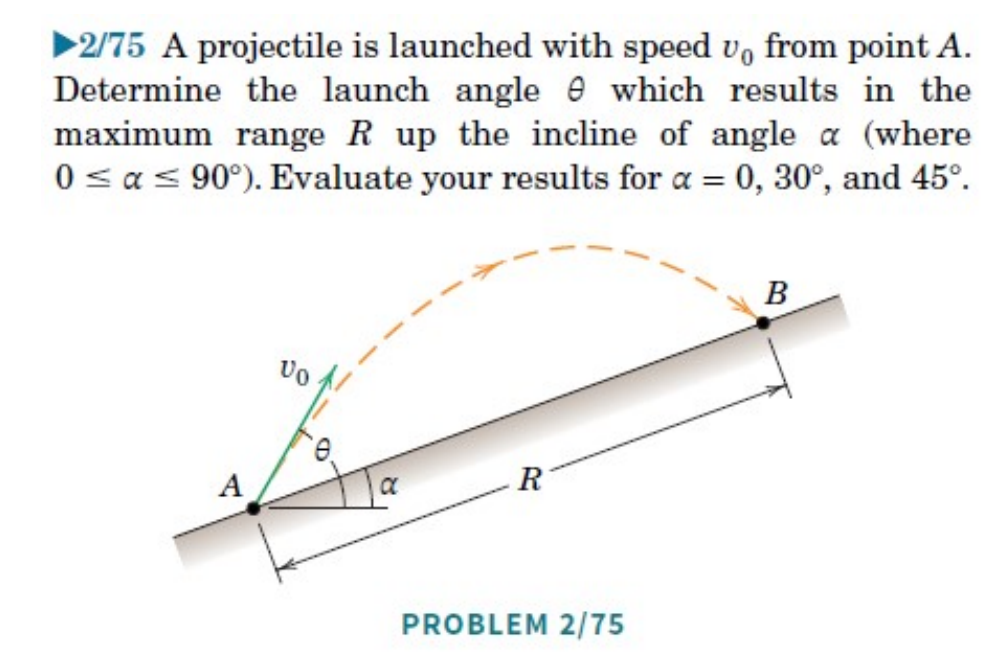
\includegraphics[width=0.5\linewidth,height=\textheight,keepaspectratio]{particle_dynamics/../figures/particle_kinetics/02-075.png}

}

\caption{MKB 2/75.}

\end{figure}%

\textbf{2.} {[}MKB 3/004{]} Consider the whole truck system; follow the
4 steps to find the truck's acceleration, then isolate a trailer to find
the drawbar tension. \emph{(ans. \(T = 13.33\) kN, \(a = 0.667\)
m/s\(^2\))}

\begin{figure}[H]

{\centering 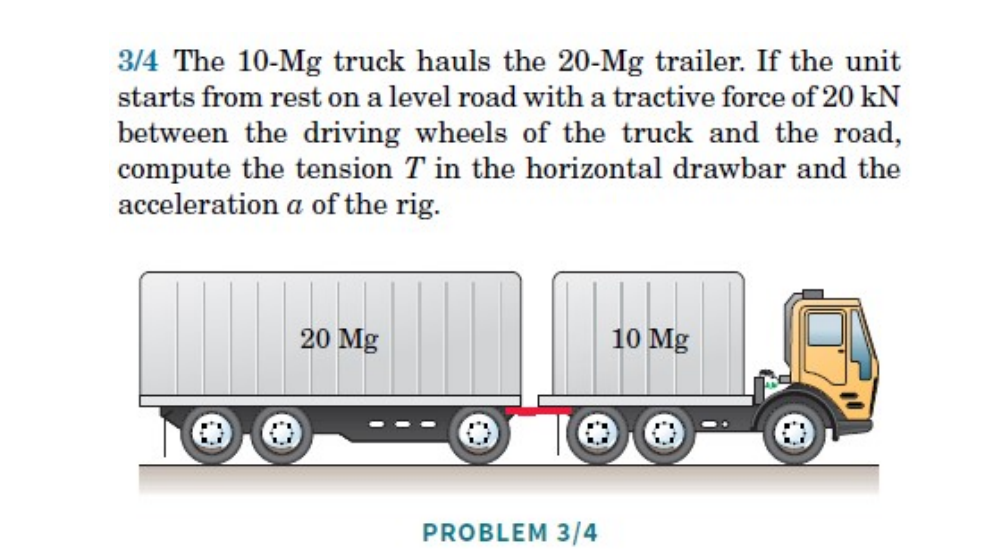
\includegraphics[width=0.5\linewidth,height=\textheight,keepaspectratio]{particle_dynamics/../figures/particle_kinetics/03-004.png}

}

\caption{MKB 3/004.}

\end{figure}%

\url{https://youtu.be/LAl3ZUiUpus}

\textbf{3.} {[}MKB 3/005{]} For each part, determine your system and
follow the 4 steps. \emph{(ans. \(R = 846\) N, \(L = 110.4\) N)}

\begin{figure}[H]

{\centering 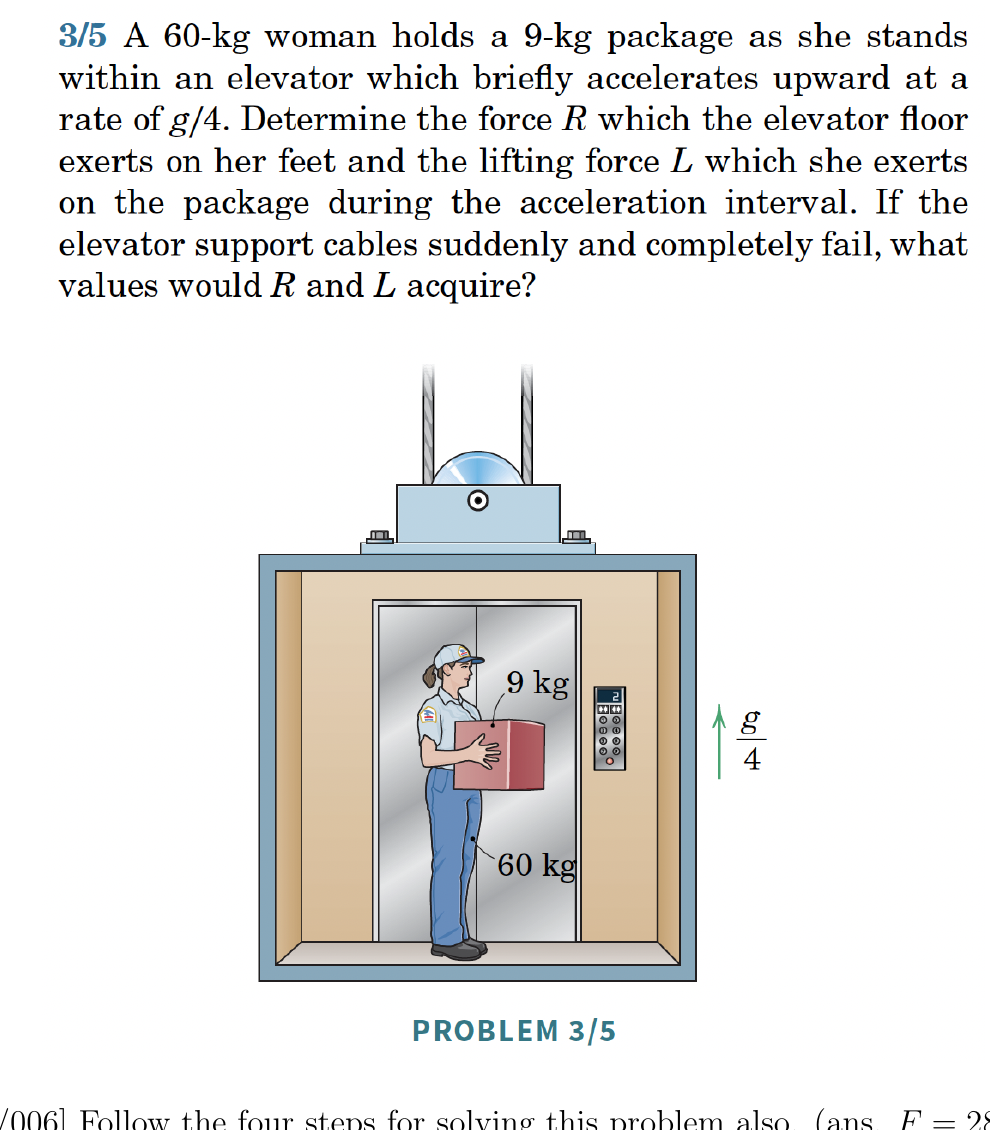
\includegraphics[width=0.5\linewidth,height=\textheight,keepaspectratio]{particle_dynamics/../figures/particle_kinetics/03-005.png}

}

\caption{MKB 3/005.}

\end{figure}%

\textbf{4.} {[}MKB 3/006{]} Follow the four steps. \emph{(ans.
\(F = 2890\) N)}

\begin{figure}[H]

{\centering 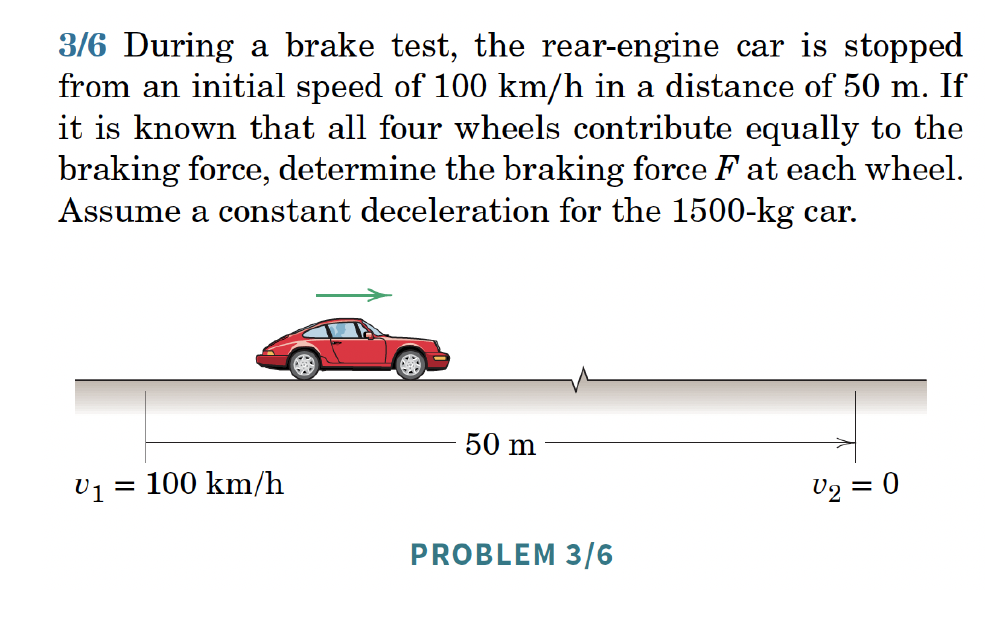
\includegraphics[width=0.5\linewidth,height=\textheight,keepaspectratio]{particle_dynamics/../figures/particle_kinetics/03-006.png}

}

\caption{MKB 3/006.}

\end{figure}%

\textbf{5.} {[}OOR Exercise 1.3{]}

\begin{figure}[H]

{\centering 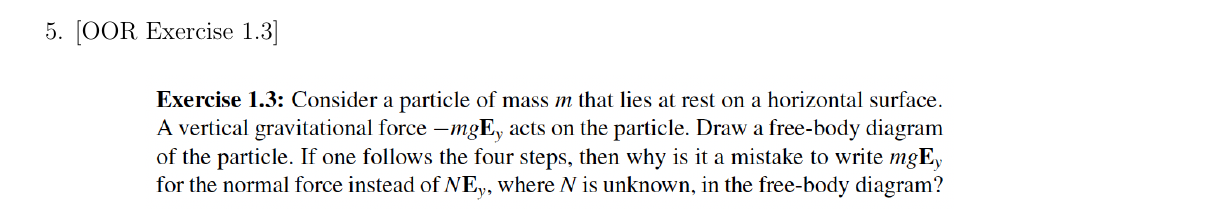
\includegraphics[width=0.7\linewidth,height=\textheight,keepaspectratio]{particle_dynamics/../figures/particle_kinetics/oor_ex_1_3.png}

}

\caption{O'Reilly Primer, Exercise 1.3.}

\end{figure}%

\textbf{6.} {[}OOR Exercise 1.5{]}

\begin{figure}[H]

{\centering 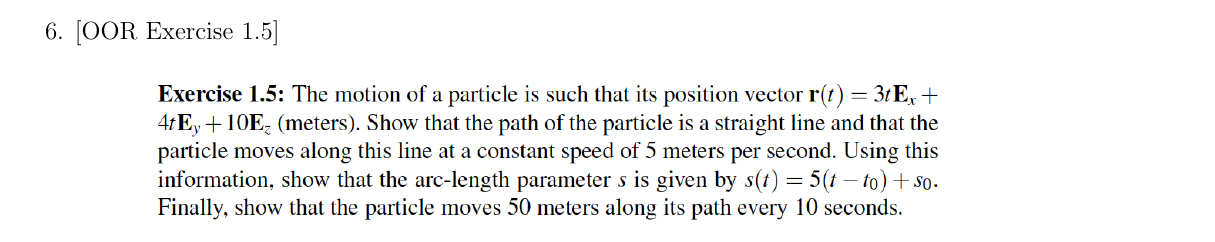
\includegraphics[width=0.7\linewidth,height=\textheight,keepaspectratio]{particle_dynamics/../figures/particle_kinetics/oor_ex_1_5.png}

}

\caption{O'Reilly Primer, Exercise 1.5.}

\end{figure}%

\textbf{7.} {[}OOR Exercise 1.8{]}

\begin{figure}[H]

{\centering 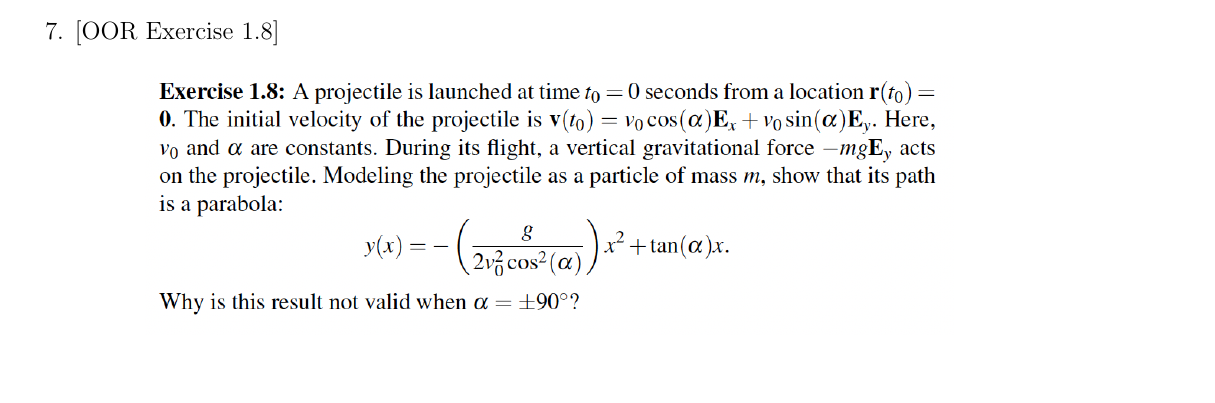
\includegraphics[width=0.7\linewidth,height=\textheight,keepaspectratio]{particle_dynamics/../figures/particle_kinetics/oor_ex_1_8.png}

}

\caption{O'Reilly Primer, Exercise 1.8.}

\end{figure}%

\chapter{Cylindrical Polar Coordinate
System}\label{cylindrical-polar-coordinate-system}

The cylindrical polar coordinate system is three-dimensional. We start
by introducing the two-dimensional polar basis, then extend it to three
dimensions.

\section{Polar Basis}\label{polar-basis}

\begin{center}
\pandocbounded{
\includegraphics[keepaspectratio]{particle_dynamics/cylindrical_polar_coordinates_files/figure-pdf/unnamed-chunk-1-1.pdf}}
\end{center}

Consider a particle in motion in the two dimensional Euclidean space
\(\mathbb{E}^2\). Define: \begin{align}
    r = \sqrt{x^2+y^2}\geq 0, \qquad \theta = \tan^{-1}\lp\frac{y}{x}\rp.
\end{align} So \begin{align}
    x = r\cos(\theta), \qquad y = r\sin(\theta)
\end{align}

Define the basis \(\{{\bf e}_r,{\bf e}_\theta\}\) as a rotation of
\(\{{\bf E}_x,{\bf E}_y\}\) by angle \(\theta\) (positive CCW about
\({\bf E}_z\)):

\begin{center}
\pandocbounded{
\includegraphics[keepaspectratio]{particle_dynamics/cylindrical_polar_coordinates_files/figure-pdf/unnamed-chunk-2-1.pdf}}
\end{center}

\begin{tcolorbox}[enhanced jigsaw, arc=.35mm, bottomrule=.15mm, bottomtitle=1mm, breakable, colback=white, colbacktitle=quarto-callout-tip-color!10!white, colframe=quarto-callout-tip-color-frame, coltitle=black, left=2mm, leftrule=.75mm, opacityback=0, opacitybacktitle=0.6, rightrule=.15mm, title=\textcolor{quarto-callout-tip-color}{\faLightbulb}\hspace{0.5em}{Think!}, titlerule=0mm, toprule=.15mm, toptitle=1mm]

\textbf{Question:} Express \({\bf e}_r\) and \({\bf e}_\theta\) in the
Cartesian basis.

\begin{quote}
\textbf{Answer}

\begin{align}
    {\bf e}_r &= \cos(\theta){\bf E}_x+\sin(\theta){\bf E}_y,\\
    {\bf e}_\theta &= -\sin(\theta){\bf E}_x+\cos(\theta){\bf E}_y.
\end{align}
\end{quote}

\end{tcolorbox}

\(\{{\bf e}_r,{\bf e}_\theta\}\) is an orthonormal basis:
\({\bf e}_r\cdot{\bf e}_r = 1\),
\({\bf e}_\theta\cdot{\bf e}_\theta = 1\),
\({\bf e}_r\cdot{\bf e}_\theta=0\).

\begin{itemize}
\tightlist
\item
  \({\bf e}_r\) points in the direction of increasing \(r\).
\item
  \({\bf e}_\theta\) points in the direction of increasing \(\theta\).
\end{itemize}

\begin{tcolorbox}[enhanced jigsaw, arc=.35mm, bottomrule=.15mm, bottomtitle=1mm, breakable, colback=white, colbacktitle=quarto-callout-tip-color!10!white, colframe=quarto-callout-tip-color-frame, coltitle=black, left=2mm, leftrule=.75mm, opacityback=0, opacitybacktitle=0.6, rightrule=.15mm, title=\textcolor{quarto-callout-tip-color}{\faLightbulb}\hspace{0.5em}{Think!}, titlerule=0mm, toprule=.15mm, toptitle=1mm]

\textbf{Question:} Calculate
\(\dot{\bf e}_r (=\dot{\theta}{\bf e}_\theta)\) and
\(\dot{\bf e}_\theta (= \dot{\bf e}_r)\).

\begin{quote}
\textbf{Answer}

\begin{align}
    \begin{split}
        {\bf e}_r = {\bf e}_r(\theta) &\implies \frac{d{\bf e}_r}{d\theta} = -\sin(\theta){\bf E}_x+\cos(\theta){\bf E}_y = {\bf e}_\theta\\
        {\bf e}_\theta = {\bf e}_\theta(\theta) &\implies \frac{d{\bf e}_\theta}{d\theta} = -\cos(\theta){\bf E}_x-\sin(\theta){\bf E}_y = -{\bf e}_r
    \end{split}
\end{align}
\end{quote}

\end{tcolorbox}

You can also see this result geometrically,

\begin{center}
\pandocbounded{
\includegraphics[keepaspectratio]{particle_dynamics/cylindrical_polar_coordinates_files/figure-pdf/unnamed-chunk-3-1.pdf}}
\end{center}

Thus, for small \(d\theta>0\), \begin{align}
    \begin{split}
        {\bf e}_r(\theta+d\theta)-{\bf e}_r(\theta) &\text{ points in the direction of }{\bf e}_\theta(\theta)\\ 
        {\bf e}_\theta(\theta+d\theta)-{\bf e}_\theta(\theta) &\text{ points in the direction of }-{\bf e}_r(\theta)
    \end{split}
\end{align}

\url{https://www.youtube.com/watch?v=r3lLIkWfMVk}

\section{Kinematics in Polar
Coordinates}\label{kinematics-in-polar-coordinates}

We can write the position vector to the particle as
\({\bf r} = r{\bf e}_r\) (with \(r\geq 0\)). Note that \({\bf e}_r\) is
a function of \(\theta\). Both \(r\) and \(\theta\) are functions of
time \(t\).

\begin{tcolorbox}[enhanced jigsaw, arc=.35mm, bottomrule=.15mm, bottomtitle=1mm, breakable, colback=white, colbacktitle=quarto-callout-tip-color!10!white, colframe=quarto-callout-tip-color-frame, coltitle=black, left=2mm, leftrule=.75mm, opacityback=0, opacitybacktitle=0.6, rightrule=.15mm, title=\textcolor{quarto-callout-tip-color}{\faLightbulb}\hspace{0.5em}{Think!}, titlerule=0mm, toprule=.15mm, toptitle=1mm]

\textbf{Question:} Show that
\({\bf v} = \dot{r}{\bf e}_r+r\dot{\theta}{\bf e}_\theta\) and
\({\bf a} = \lp \ddot{r}-r\dot{\theta}^2\rp{\bf e}_r+\lp 2\dot{r}\dot{\theta}+r\ddot{\theta}\rp{\bf e}_\theta\).

\begin{quote}
\textbf{Answer}

\begin{align*}
    {\bf v} &= \dot{r}{\bf e}_r+r\dot{\bf e}_r\\
    &= \dot{r}{\bf e}_r+r\frac{d{\bf e}_r}{d\theta}\dot{\theta}\\
    &= \dot{r}{\bf e}_r+r\dot{\theta}{\bf e}_\theta.\\
    {\bf a} &= \ddot{r}{\bf e}_r+\dot{r}\dot{\bf e}_r+\dot{r}\dot{\theta}{\bf e}_\theta+r\ddot{\theta}{\bf e}_\theta+r\dot{\theta}\dot{\bf e}_\theta\\
    &= \lp \ddot{r}-r\dot{\theta}^2\rp{\bf e}_r+\lp 2\dot{r}\dot{\theta}+r\ddot{\theta}\rp{\bf e}_\theta.
\end{align*}
\end{quote}

\end{tcolorbox}

Note the components of acceleration vector:

\begin{itemize}
\tightlist
\item
  \(r\ddot{\theta}\): tangential
\item
  \(\ddot{r}\): radial
\item
  \(r\dot{\theta}^2\): centripetal
\item
  \(2\dot{r}\dot{\theta}\): Coriolis
\end{itemize}

We may also introduce the notation \begin{align*}
    {\bf r} &= r{\bf e}_r+0{\bf e}_\theta\\
    {\bf v} &= v_r{\bf e}_r+v_\theta{\bf e}_\theta\\
    {\bf a} &= a_r{\bf e}_r+a_\theta{\bf e}_\theta
\end{align*}

\textbf{Remark: \(a_r \neq \dot{v}_r\).} Be careful: \(v_r = \dot{r}\)
so \(\dot{v}_r = \ddot{r}\), but
\(a_r = \ddot{r} - r\dot{\theta}^2 \neq \dot{v}_r\) in general.

\textbf{Remark: When to use polar vs Cartesiancoordinates?} For
rectilinear motions, Cartesian coordinates are usually easiest. For
problems where \(r\) is directly measured (e.g.~radar tracking as in MKB
2/121.), polar coordinates are natural.

\begin{figure}[H]

{\centering 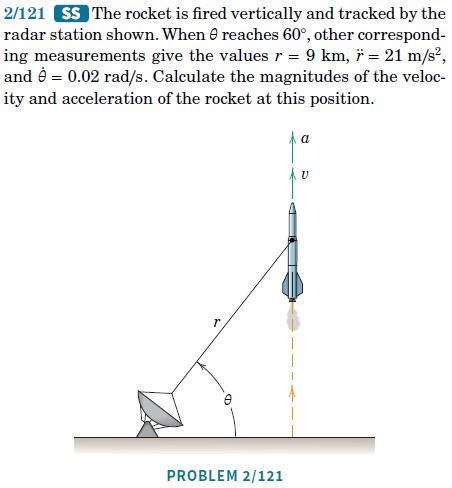
\includegraphics[width=0.5\linewidth,height=\textheight,keepaspectratio]{particle_dynamics/../figures/cylindrical_polar_coordinates/02-121.jpg}

}

\caption{MKB 2/121.}

\end{figure}%

\section{Example: Nonlinear Pendulum}\label{example-nonlinear-pendulum}

Consider a particle of mass \(m\) suspended by a massless inextensible
string of length \(\ell\). Find the equation of motion of the particle
and the tension in the string.

\begin{center}
\pandocbounded{
\includegraphics[keepaspectratio]{particle_dynamics/cylindrical_polar_coordinates_files/figure-pdf/unnamed-chunk-4-1.pdf}}
\end{center}

The planar motion of the particle is constrained by the string. This
constraint can be expressed mathematically in Cartesian and polar
coordinates respectively as \begin{align}
    \sqrt{x^2+y^2} = \ell
\end{align} \begin{align}
    r = \ell = \text{const.} \implies \dot{r}=0,\ \ddot{r} = 0.
\end{align} Note that the constraint is simpler in polar coordinates.
This is a common theme: the right choice of coordinates can simplify the
problem significantly.

\begin{tcolorbox}[enhanced jigsaw, arc=.35mm, bottomrule=.15mm, bottomtitle=1mm, breakable, colback=white, colbacktitle=quarto-callout-tip-color!10!white, colframe=quarto-callout-tip-color-frame, coltitle=black, left=2mm, leftrule=.75mm, opacityback=0, opacitybacktitle=0.6, rightrule=.15mm, title=\textcolor{quarto-callout-tip-color}{\faLightbulb}\hspace{0.5em}{Think!}, titlerule=0mm, toprule=.15mm, toptitle=1mm]

\textbf{Question:} How many degrees of freedom does this system have?

\begin{quote}
\textbf{Answer}

One. A particle in the plane has 2 DOFs, but the constraint \(r=\ell\)
removes one. Knowing \(\theta(t)\) completely describes the motion.
\end{quote}

\end{tcolorbox}

Following the four steps:

\begin{enumerate}
\def\labelenumi{\arabic{enumi}.}
\tightlist
\item
  Our system is the particke. Choosing polar coordinates, we write its
  position, velocity, and acceleration as \begin{align*}
   {\bf r} &= \ell{\bf e}_r, \quad {\bf v} = \ell\dot{\theta}{\bf e}_\theta, \quad {\bf a} = \ell\ddot{\theta}{\bf e}_\theta-\ell\dot{\theta}^2{\bf e}_r.
  \end{align*}
\end{enumerate}

\begin{tcolorbox}[enhanced jigsaw, arc=.35mm, bottomrule=.15mm, bottomtitle=1mm, breakable, colback=white, colbacktitle=quarto-callout-note-color!10!white, colframe=quarto-callout-note-color-frame, coltitle=black, left=2mm, leftrule=.75mm, opacityback=0, opacitybacktitle=0.6, rightrule=.15mm, title=\textcolor{quarto-callout-note-color}{\faInfo}\hspace{0.5em}{Orienting \({\bf e}_\theta\)}, titlerule=0mm, toprule=.15mm, toptitle=1mm]

\({\bf e}_\theta\) points in the direction of increasing \(\theta\),
determined by the right-hand rule: point the thumb along \({\bf E}_z\);
your fingers curl in the direction of increasing \(\theta\).

\end{tcolorbox}

\begin{enumerate}
\def\labelenumi{\arabic{enumi}.}
\setcounter{enumi}{1}
\tightlist
\item
  Forces: \begin{align*}
   {\bf T} &= T\lp-{\bf e}_r\rp, \quad {\bf W} = mg\lp\cos(\theta){\bf e}_r-\sin(\theta){\bf e}_\theta\rp.
  \end{align*}
\end{enumerate}

\begin{tcolorbox}[enhanced jigsaw, arc=.35mm, bottomrule=.15mm, bottomtitle=1mm, breakable, colback=white, colbacktitle=quarto-callout-note-color!10!white, colframe=quarto-callout-note-color-frame, coltitle=black, left=2mm, leftrule=.75mm, opacityback=0, opacitybacktitle=0.6, rightrule=.15mm, title=\textcolor{quarto-callout-note-color}{\faInfo}\hspace{0.5em}{Remark: Tension}, titlerule=0mm, toprule=.15mm, toptitle=1mm]

\({\bf T}\) is a constraint force keeping the particle on a circular
path. If \(T>0\), the wire is in tension. The tension is the same
throughout because the wire is massless.

\end{tcolorbox}

\begin{enumerate}
\def\labelenumi{\arabic{enumi}.}
\setcounter{enumi}{2}
\item
  Balance of linear momentum: \begin{align*}
   mg{\bf E}_x-T{\bf e}_r &= m\ell\lp\ddot{\theta}{\bf e}_\theta-\dot{\theta}^2{\bf e}_r\rp.
  \end{align*}
\item
  Projecting along \({\bf e}_\theta\) (hides unknown tension) and
  results in the equation of motion for \(\theta\): \begin{align*}
   -mg\sin(\theta) &= m\ell\ddot{\theta} \implies \ddot{\theta}+\frac{g}{\ell}\sin(\theta) = 0
  \end{align*} which can be solved numerically for \(\theta(t)\) given
  IC's \(\theta(0), \dot{\theta}(0)\). This is a nonlinear ODE. For
  small \(\theta\), we can linearise \(\sin(\theta)\approx \theta\) and
  solve the resulting simple harmonic motion equation by hand
  \begin{align*}
   \ddot{\theta}+\frac{g}{\ell}\theta = 0
  \end{align*}
\end{enumerate}

Projecting along \({\bf e}_r\) gives the tension: \begin{align*}
    T = m\lp\ell\dot{\theta}^2+g\cos(\theta)\rp
\end{align*}

\section{Types of Accelerations
Explained}\label{types-of-accelerations-explained}

The goal of this section is to give physical intuition for the different
components of acceleration in polar coordinates.

Recall: \begin{align*}
    {\bf a} = \lp\ddot{r}-r\dot{\theta}^2\rp{\bf e}_r+\lp2\dot{r}\dot{\theta}+r\ddot{\theta}\rp{\bf e}_\theta.
\end{align*}

\begin{tcolorbox}[enhanced jigsaw, arc=.35mm, bottomrule=.15mm, bottomtitle=1mm, breakable, colback=white, colbacktitle=quarto-callout-tip-color!10!white, colframe=quarto-callout-tip-color-frame, coltitle=black, left=2mm, leftrule=.75mm, opacityback=0, opacitybacktitle=0.6, rightrule=.15mm, title=\textcolor{quarto-callout-tip-color}{\faLightbulb}\hspace{0.5em}{Think!}, titlerule=0mm, toprule=.15mm, toptitle=1mm]

\textbf{Question:} Can you think of physical systems where the
acceleration of the particle is purely tangential, purely radial, purely
centripetal, or purely Coriolis?

\begin{quote}
\textbf{Answer}

\ldots{}
\end{quote}

\end{tcolorbox}

\begin{itemize}
\tightlist
\item
  \textbf{Radial} \(\ddot{r}\): particle on a spring in rectilinear
  motion.
\item
  \textbf{Centripetal} \(-r\dot{\theta}^2\): particle on a circle at
  constant speed --- the normal force steers the particle.
\item
  \textbf{Tangential} \(r\ddot{\theta}\): It is not possible to have
  purely tangential acceleration without a nonzero centripetal
  acceleration. A particle pushed along a circle with varying speed
  constitutes a minimal example that has both tangential and centripetal
  acceleration.
\item
  \textbf{Coriolis} \(2\dot{r}\dot{\theta}\): It is not possible to have
  purely Coriolis acceleration without a nonzero centripetal
  acceleration. A minimal example of nonzero Coriolis acceleration is a
  particle in a tube rotating at constant angular velocity. The Coriolis
  acceleration is due to both the rotation of the tube and the radial
  motion of the particle inside the tube.
\end{itemize}

\subsection{Example: Particle in a Rotating
Tube}\label{example-particle-in-a-rotating-tube}

Consider a particle of mass \(m\) inside a tube rotating at constant
angular velocity \(\omega\) about the vertical axis. The tube is
horizontal and frictionless. Find the equation of motion for \(r(t)\)
and the normal force on the particle.

\begin{center}
\pandocbounded{
\includegraphics[keepaspectratio]{particle_dynamics/cylindrical_polar_coordinates_files/figure-pdf/unnamed-chunk-5-1.pdf}}
\end{center}

Following the four steps:

\begin{enumerate}
\def\labelenumi{\arabic{enumi}.}
\item
  Kinematics: Here \(\dot{\theta} = \omega = \text{const.}\),
  \(\ddot{\theta} = 0\), so \begin{align*}
   {\bf r} = r{\bf e}_r, \quad {\bf v} = \dot{r}{\bf e}_r+r\omega{\bf e}_\theta, \quad {\bf a} = \lp\ddot{r}-r\omega^2\rp{\bf e}_r+2\dot{r}\omega{\bf e}_\theta.
  \end{align*}
\item
  Assume no friction: \({\bf N} = N_\theta{\bf e}_\theta+N_z{\bf E}_z\),
  \({\bf W} = -mg{\bf E}_z\).
\item
  The balance of linear momentum is \begin{align*}
   {\bf F} &= \dot{\bf G},\\
   N_\theta{\bf e}_\theta+N_z{\bf E}_z - mg{\bf E}_z &= m\lp\ddot{r}-r\omega^2\rp{\bf e}_r+2m\dot{r}\omega{\bf e}_\theta.
  \end{align*}
\item
  Projecting this equation along \({\bf e}_r\) and \({\bf e}_\theta\)
  gives, \begin{align*}
   \lp{\bf F} = \dot{\bf G}\rp\cdot{\bf e}_r &\implies \ddot{r}-\omega^2 r = 0 \quad (\text{EOM for } r(t)),\\
   \lp{\bf F} = \dot{\bf G}\rp\cdot{\bf e}_\theta &\implies N_\theta = 2m\dot{r}\omega \quad (\text{Coriolis reaction}).
  \end{align*}
\end{enumerate}

\begin{tcolorbox}[enhanced jigsaw, arc=.35mm, bottomrule=.15mm, bottomtitle=1mm, breakable, colback=white, colbacktitle=quarto-callout-note-color!10!white, colframe=quarto-callout-note-color-frame, coltitle=black, left=2mm, leftrule=.75mm, opacityback=0, opacitybacktitle=0.6, rightrule=.15mm, title=\textcolor{quarto-callout-note-color}{\faInfo}\hspace{0.5em}{Coriolis acceleration}, titlerule=0mm, toprule=.15mm, toptitle=1mm]

As the particle moves outward, \(r\omega\) increases. The tube must
supply the \({\bf e}_\theta\) acceleration \(2\dot{r}\omega\) so the
particle stays inside.

\end{tcolorbox}

\subsection{Example: Particle Pushed in a
Circle}\label{example-particle-pushed-in-a-circle}

Consider a particle of mass \(m\) on a horizontal circular guide. The
particle is pushed by a force \({\bf P}\) in the \({\bf e}_\theta\)
around the circle of radius \(R\) at constant angular velocity
\(\omega\). Find the normal force on the particle.

Following the four steps:

\begin{enumerate}
\def\labelenumi{\arabic{enumi}.}
\tightlist
\item
\end{enumerate}

\begin{align*}
    {\bf r} &= R{\bf e}_r+H{\bf E}_z\\
    {\bf v} &= R\dot{\theta}{\bf e}_\theta\\
    {\bf a} &= R\ddot{\theta}{\bf e}_\theta-R\dot{\theta}^2{\bf e}_r
\end{align*}

\begin{enumerate}
\def\labelenumi{\arabic{enumi}.}
\setcounter{enumi}{1}
\item
  The normal force \({\bf N}\) from the track has components in the
  \({\bf e}_r\) and \({\bf E}_z\) directions. \begin{align*}
   {\bf P} &= P{\bf e}_\theta\quad ({\bf P} = P{\bf E}_y \text{ only at initial instant.})\\
   {\bf W} &= mg\lp-{\bf E}_z\rp = -mg{\bf E}_z\\
   {\bf N} &= N_r\lp-{\bf e}_r\rp+N_z{\bf E}_z
  \end{align*}
\item
  The balance of linear momentum is \begin{align*}
   -N_r{\bf e}_r+\lp N_z-mg\rp{\bf E}_z+P{\bf e}_\theta = mR\lp\ddot{\theta}{\bf e}_\theta-\dot{\theta}^2{\bf e}_r\rp
  \end{align*}
\item
  Projecting along \({\bf e}_\theta\), \({\bf e}_r\), and \({\bf E}_z\)
  gives \begin{align*}
   \lp{\bf F}=\dot{G}\rp\cdot{\bf e}_\theta &\quad P=mR\ddot{\theta}\\
   \lp{\bf F}=\dot{G}\rp\cdot{\bf e}_r &\quad N_r=mR\dot{\theta}^2\\
   \lp{\bf F}=\dot{G}\rp\cdot{\bf E}_z &\quad N_z=mg
  \end{align*} The first of these equations hides \({\bf N}\) and
  provides an EOM for \(\theta(t)\) that can be solved given the ICs
  \(\theta_0, \dot{\theta}_0\).
\end{enumerate}

The second and third of these equations provide the constraint force
components. \(N_r\) supplies the centripetal acceleration which steers
the particle. \(N_z\) holds up the particle and ensure \(\ddot{z}=0\).

\section{Cylindrical-Polar
Coordinates}\label{cylindrical-polar-coordinates}

Consider a particle in motion in three-dimensional Euclidean space
\(\mathbb{E}^3\). We can extend the polar coordinate system by adding a
vertical coordinate \(z\) and a vertical basis vector \({\bf E}_z\). The
radial unit vector \({\bf e}_r\) lies along the projection of
\({\bf r}\) in the \(\{{\bf E}_x,{\bf E}_y\}\) plane.

\begin{center}
\pandocbounded{
\includegraphics[keepaspectratio]{particle_dynamics/cylindrical_polar_coordinates_files/figure-pdf/unnamed-chunk-6-1.pdf}}
\end{center}

In summary, \begin{align*}
    \begin{bmatrix}{\bf e}_r\\ {\bf e}_\theta\\ {\bf E}_z\end{bmatrix}
    =
    \begin{bmatrix}\cos(\theta) & \sin(\theta) & 0\\ -\sin(\theta) & \cos(\theta) & 0\\ 0 & 0 & 1\end{bmatrix}
    \begin{bmatrix}{\bf E}_x\\ {\bf E}_y\\ {\bf E}_z\end{bmatrix}.
\end{align*}

The position, velocity, acceleration of the particle are \begin{align*}
    {\bf r} &= r{\bf e}_r+z{\bf E}_z,\\
    {\bf v} &= \dot{r}{\bf e}_r+r\dot{\theta}{\bf e}_\theta+\dot{z}{\bf E}_z,\\
    {\bf a} &= \lp\ddot{r}-r\dot{\theta}^2\rp{\bf e}_r+\lp2\dot{r}\dot{\theta}+r\ddot{\theta}\rp{\bf e}_\theta+\ddot{z}{\bf E}_z.
\end{align*}

\section{Summary}\label{summary-3}

\textbf{Cylindrical polar basis}
\(\{\mathbf{e}_r,\mathbf{e}_\theta,\mathbf{E}_z\}\): \begin{align}
    \mathbf{e}_r &= \cos\theta\,\mathbf{E}_x+\sin\theta\,\mathbf{E}_y, &
    \mathbf{e}_\theta &= -\sin\theta\,\mathbf{E}_x+\cos\theta\,\mathbf{E}_y, \\
    \dot{\mathbf{e}}_r &= \dot\theta\,\mathbf{e}_\theta, &
    \dot{\mathbf{e}}_\theta &= -\dot\theta\,\mathbf{e}_r.
\end{align}

\textbf{Position, velocity, acceleration:} \begin{align}
    \mathbf{r} &= r\mathbf{e}_r+z\mathbf{E}_z,\\
    \mathbf{v} &= \dot r\,\mathbf{e}_r + r\dot\theta\,\mathbf{e}_\theta + \dot z\,\mathbf{E}_z,\\
    \mathbf{a} &= (\ddot r-r\dot\theta^2)\mathbf{e}_r + (r\ddot\theta+2\dot r\dot\theta)\mathbf{e}_\theta + \ddot z\,\mathbf{E}_z.
\end{align}

\section{Lecture Videos}\label{lecture-videos}

\url{https://youtu.be/pj7kitk0VcI}

\section{Exercises}\label{exercises-5}

In both the following problems, set up a cylindrical polar coordinate
system whose origin is taken to be at the vertex of the cone.

\textbf{a.}

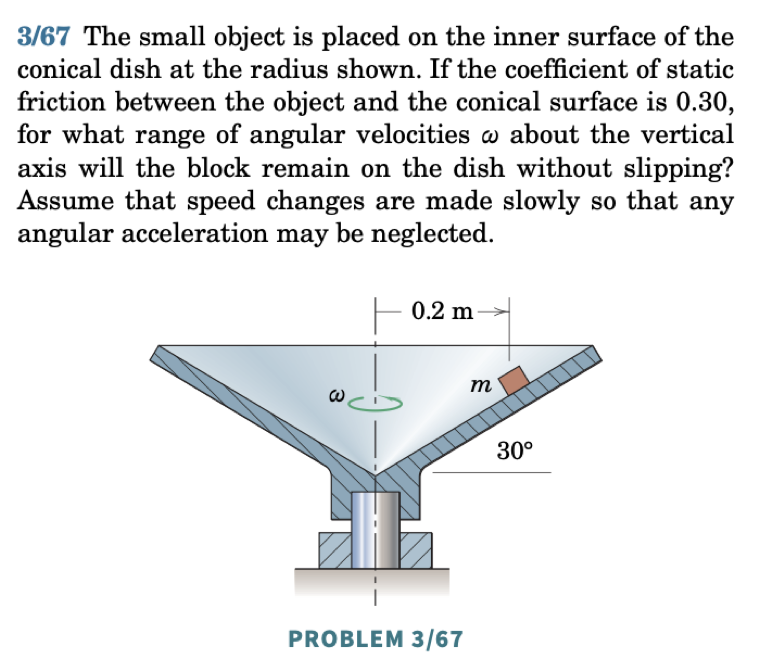
\includegraphics[width=0.5\linewidth,height=\textheight,keepaspectratio]{particle_dynamics/../figures/cylindrical_polar_coordinates/03-067.png}

See an animation of the cylindrical-polar basis for a particle moving
aroubd a cone
\href{https://drive.google.com/file/d/1d8FJqs0GMQU0FxUE3R66rfcSTCCHFTOu/view?usp=sharing}{here}.

\textbf{b.}

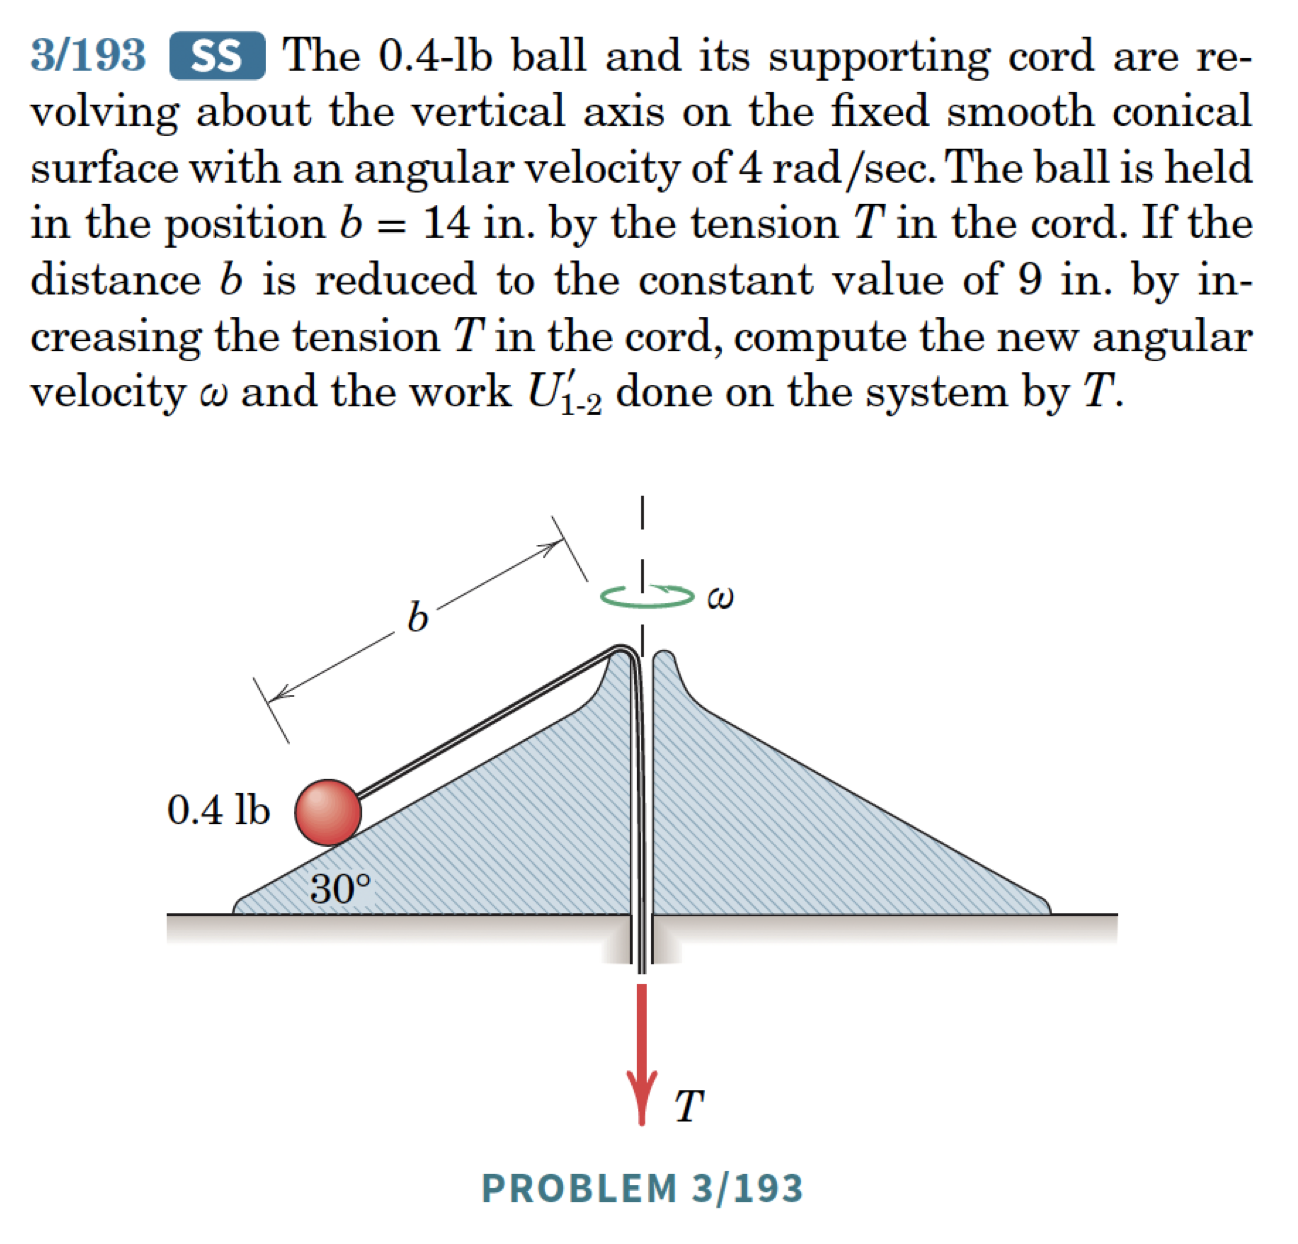
\includegraphics[width=0.5\linewidth,height=\textheight,keepaspectratio]{particle_dynamics/../figures/cylindrical_polar_coordinates/03-193.png}

\emph{The following problems are from Set 05 -- Cylindrical Polar
Coordinates.}

\textbf{1.} {[}MKB 2/121{]} Take the origin at the satellite;
\(\mathbf{E}_x\) rightwards, \(\mathbf{E}_y\) upwards. Write the
position in both cylindrical and Cartesian coordinates. \emph{(ans.
\(v = 360\) m/s, \(a = 20.1\) m/s\(^2\))}

\begin{figure}[H]

{\centering 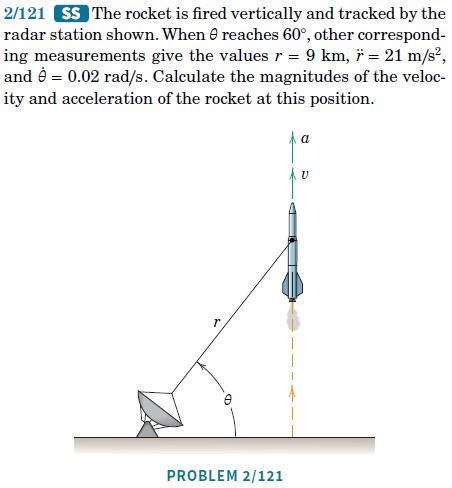
\includegraphics[width=0.5\linewidth,height=\textheight,keepaspectratio]{particle_dynamics/../figures/cylindrical_polar_coordinates/02-121.jpg}

}

\caption{MKB 2/121.}

\end{figure}%

\url{https://youtu.be/wbUBexp8xfc}

\textbf{2.} {[}MKB 02-105{]} Take \(\mathbf{E}_x\) rightwards and
\(\mathbf{E}_y\) upwards; write the car's position in both bases.
\emph{(ans. \(\dot r = 47.7\) ft/sec, \(\dot\theta = -41.0\) deg/sec)}

\begin{figure}[H]

{\centering 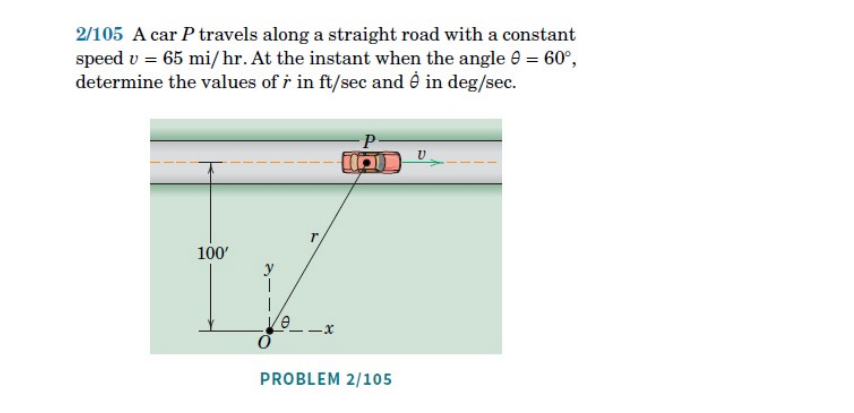
\includegraphics[width=0.5\linewidth,height=\textheight,keepaspectratio]{particle_dynamics/../figures/cylindrical_polar_coordinates/02-105.png}

}

\caption{MKB 02-105.}

\end{figure}%

\textbf{3.} {[}MKB 02-126{]} Write
\(\mathbf{r}_P = (0.75+\ell)\mathbf{e}_r\) m and differentiate. If the
setup is in the vertical plane, find the force applied by the robot arm.
\emph{(ans. \(v=0.296\) m/s, \(a=0.345\) m/s\(^2\))}

\begin{figure}[H]

{\centering 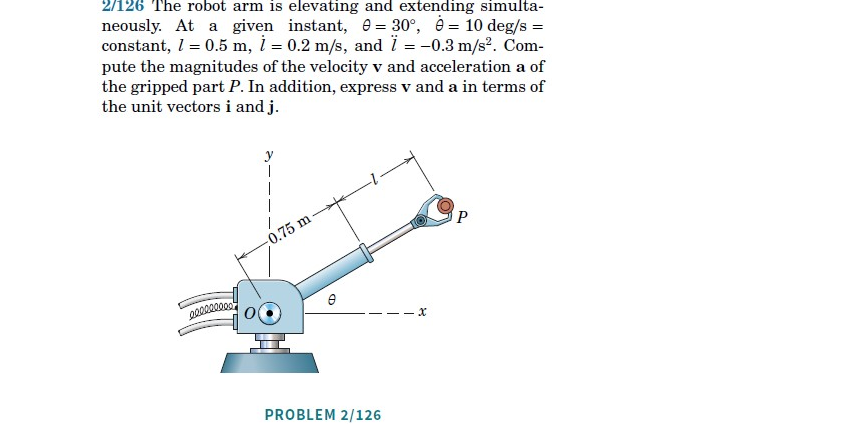
\includegraphics[width=0.5\linewidth,height=\textheight,keepaspectratio]{particle_dynamics/../figures/cylindrical_polar_coordinates/02-126.png}

}

\caption{MKB 02-126.}

\end{figure}%

\textbf{4.} {[}MKB 03-037{]} Apply the 4 steps at points \(A\) and \(B\)
independently; origin at the centre of curvature. \emph{(ans.
\(N_A = 10.89\) N, \(N_B = 8.30\) N)}

\begin{figure}[H]

{\centering 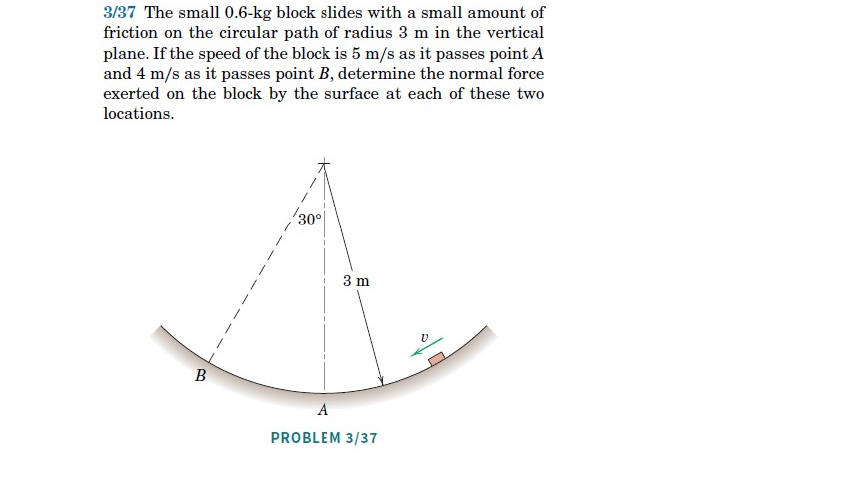
\includegraphics[width=0.5\linewidth,height=\textheight,keepaspectratio]{particle_dynamics/../figures/cylindrical_polar_coordinates/03-037.png}

}

\caption{MKB 03-037.}

\end{figure}%

\textbf{5.} {[}Primer Exercise 2.6{]}

\begin{figure}[H]

{\centering 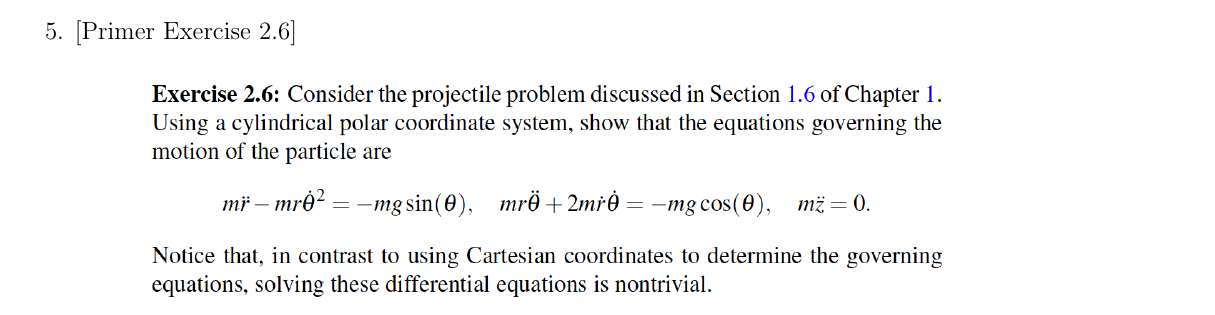
\includegraphics[width=0.7\linewidth,height=\textheight,keepaspectratio]{particle_dynamics/../figures/cylindrical_polar_coordinates/oor_ex_2_6.png}

}

\caption{O'Reilly Primer, Exercise 2.6.}

\end{figure}%

\textbf{6.} {[}Primer Exercise 2.7{]}

\begin{figure}[H]

{\centering 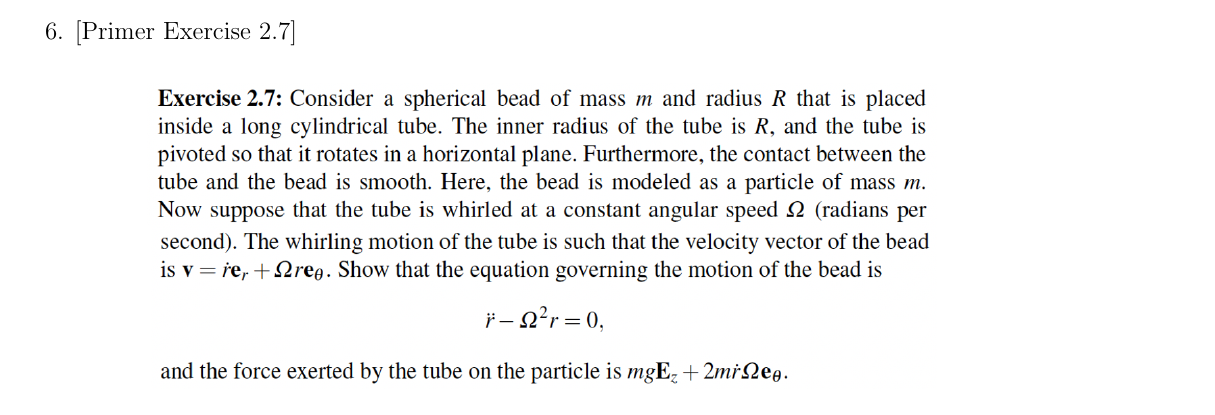
\includegraphics[width=0.7\linewidth,height=\textheight,keepaspectratio]{particle_dynamics/../figures/cylindrical_polar_coordinates/oor_ex_2_7.png}

}

\caption{O'Reilly Primer, Exercise 2.7.}

\end{figure}%

\textbf{7.} {[}Primer Exercise 2.8{]}

\begin{figure}[H]

{\centering 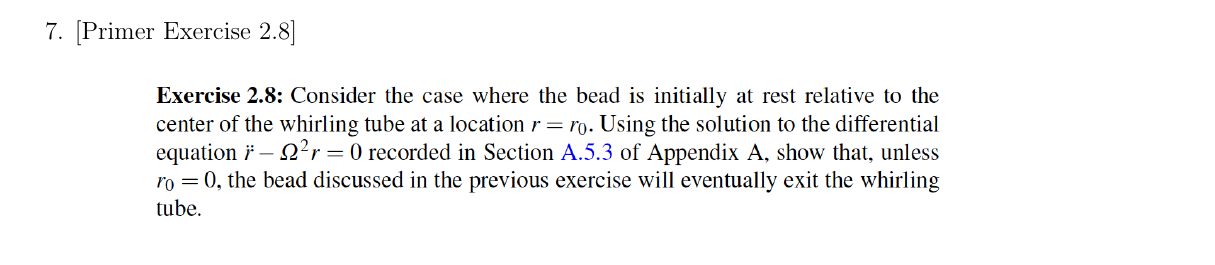
\includegraphics[width=0.7\linewidth,height=\textheight,keepaspectratio]{particle_dynamics/../figures/cylindrical_polar_coordinates/oor_ex_2_8.png}

}

\caption{O'Reilly Primer, Exercise 2.8.}

\end{figure}%

\chapter{Constrained Motion}\label{constrained-motion}

The \textbf{degree of freedom (DOF)} of a system is the number of
independent coordinates needed to describe a configuration of the
system.

Examples:

\begin{itemize}
\tightlist
\item
  A particle free to move in \(\mathbb{E}^2\) has 2 DOFs.
\item
  A particle constrained to move on a curve in \(\mathbb{E}^2\) has 1
  DOF.
\item
  Two particles free to move in \(\mathbb{E}^2\) have a combined total
  of 4 DOFs.
\item
  If two particles in \(\mathbb{E}^2\) are constrained to move on the
  same curve, they have 2 DOFs.
\item
  If two particles in \(\mathbb{E}^2\) are connected by a rigid rod,
  they have 3 DOFs. The constraint
  \(\lnorm{\bf r}_{B/A}\rnorm = l\,\forall t\) provides a relationship
  between their coordinates that eliminates one DOF.
\item
  If two particles in \(\mathbb{E}^2\) are connected by a rigid rod and
  constrained to move on a curve, they have 1 DOF.
\end{itemize}

\begin{center}\rule{0.5\linewidth}{0.5pt}\end{center}

\textbf{Example:} Consider two particles in smooth vertical slots. If
\(A\) and \(B\) move independently, the system has 2 DOFs. If connected
by an inextensible cable, the system has 1 DOF.

The inextensibility constraint \(\ell = \text{const.}\) can be written
as: \begin{align}
    & \ell = s_A+c+s_B\\
    & \Delta \ell = 0 = \Delta_{t_1\rightarrow t_2} s_A+\Delta_{t_1\rightarrow t_2} s_B\\
    & \implies \Delta s_B = -\Delta s_A\\
    & \dot{\ell} = 0 = \dot{s}_A+\dot{s}_B\\
    & \implies \dot{s}_B=-\dot{s}_A.
\end{align}

\begin{center}
\pandocbounded{
\includegraphics[keepaspectratio]{particle_dynamics/constrained_motion_files/figure-pdf/unnamed-chunk-1-1.pdf}}
\end{center}

\section{Summary}\label{summary-4}

For \textbf{pulley--chord systems}: (1) choose a datum, (2) define
distances from the datum, (3) write a chord equation per chord. Each
chord equation and its derivatives give additional constraints.

\section{Exercises}\label{exercises-6}

\emph{The following problems are from Set 06 -- Constrained Motion.}

\textbf{1.} {[}MKB 2/099{]} Determine the \(\mathbf{e}_r\) and
\(\mathbf{e}_\theta\) components of the acceleration of pin \(P\);
origin at the centre of the circular slot. \emph{(ans. \(a_n = 66.0\)
mm/s\(^2\), \(a_t = 29.7\) mm/s\(^2\))}

\begin{figure}[H]

{\centering 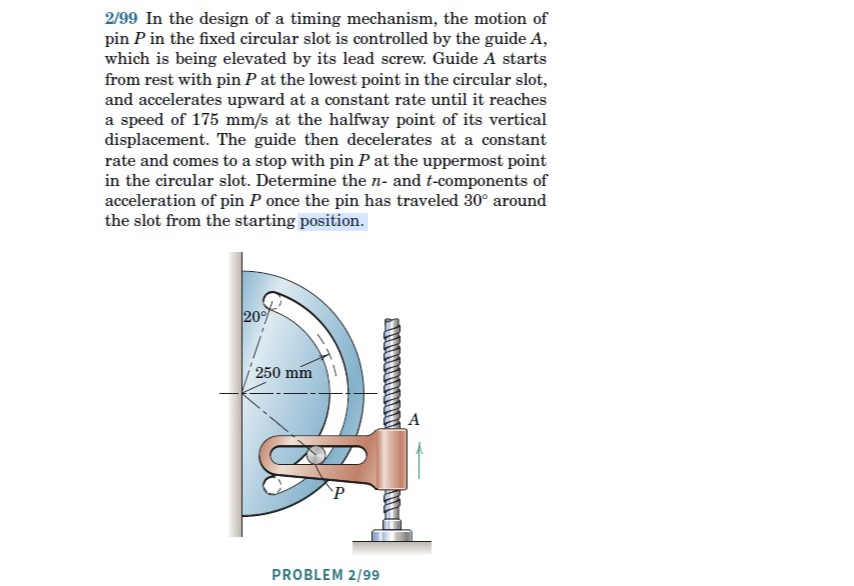
\includegraphics[width=0.5\linewidth,height=\textheight,keepaspectratio]{particle_dynamics/../figures/constrained_motion/02-099.png}

}

\caption{MKB 2/099.}

\end{figure}%

\url{https://youtu.be/Bt5neJj4Zhc}

\textbf{2.} {[}03-056{]} Set up two polar coordinate systems with
origins \(O\) and \(O'\). Write position vectors of \(P\) in each basis.
\emph{(ans. \(N = 2.89\) N towards \(O'\), \(R = 1.599\) N)}

\begin{figure}[H]

{\centering 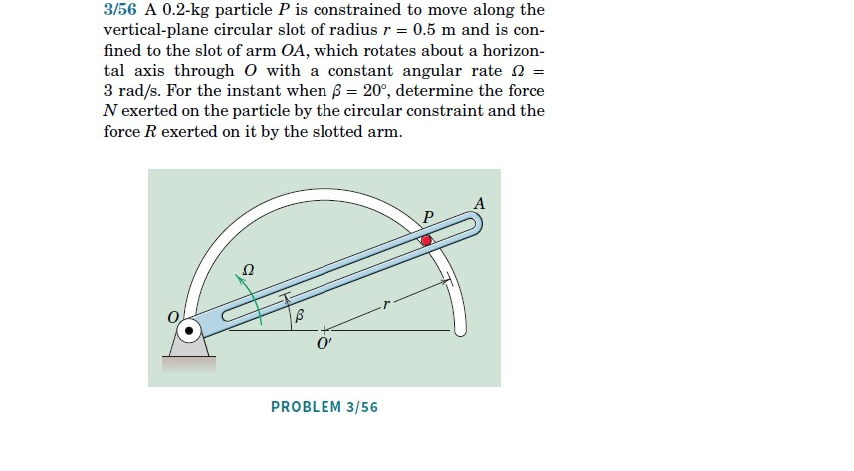
\includegraphics[width=0.5\linewidth,height=\textheight,keepaspectratio]{particle_dynamics/../figures/constrained_motion/03-056.png}

}

\caption{MKB 03-056.}

\end{figure}%

\textbf{3.} {[}MKB 02-172{]} Use
\(\mathbf{v}_{B/A}=\mathbf{v}_B-\mathbf{v}_A=3.5\mathbf{E}_y\) m/s.
\emph{(ans. \(\mathbf{v}_A=-0.5\mathbf{E}_y\) m/s,
\(\mathbf{v}_B=3\mathbf{E}_y\) m/s)}

\begin{figure}[H]

{\centering 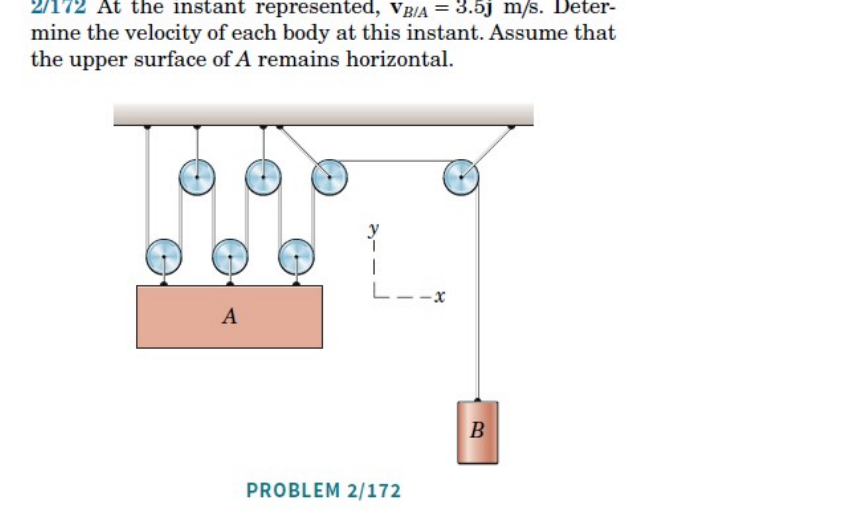
\includegraphics[width=0.5\linewidth,height=\textheight,keepaspectratio]{particle_dynamics/../figures/constrained_motion/02-172.png}

}

\caption{MKB 02-172.}

\end{figure}%

\textbf{4.} {[}MKB 03-021{]} Draw FBDs of the massless pulleys to find
forces on the 60-lb cylinders. \emph{(ans. (a) \(a=10.73\) ft/sec\(^2\)
up; (b) \(a=2.93\) ft/sec\(^2\) up)}

\begin{figure}[H]

{\centering 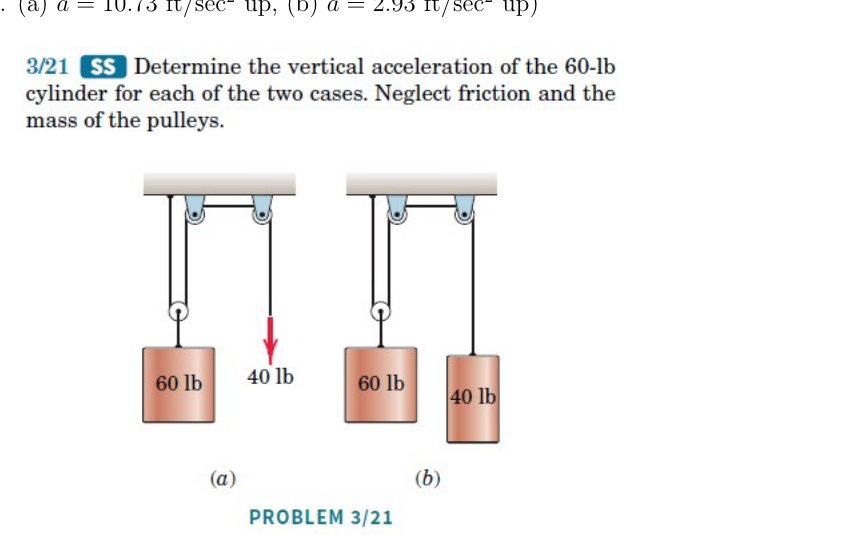
\includegraphics[width=0.5\linewidth,height=\textheight,keepaspectratio]{particle_dynamics/../figures/constrained_motion/03-021.png}

}

\caption{MKB 03-021.}

\end{figure}%

\textbf{5.} {[}MKB 2-177{]}

\begin{figure}[H]

{\centering 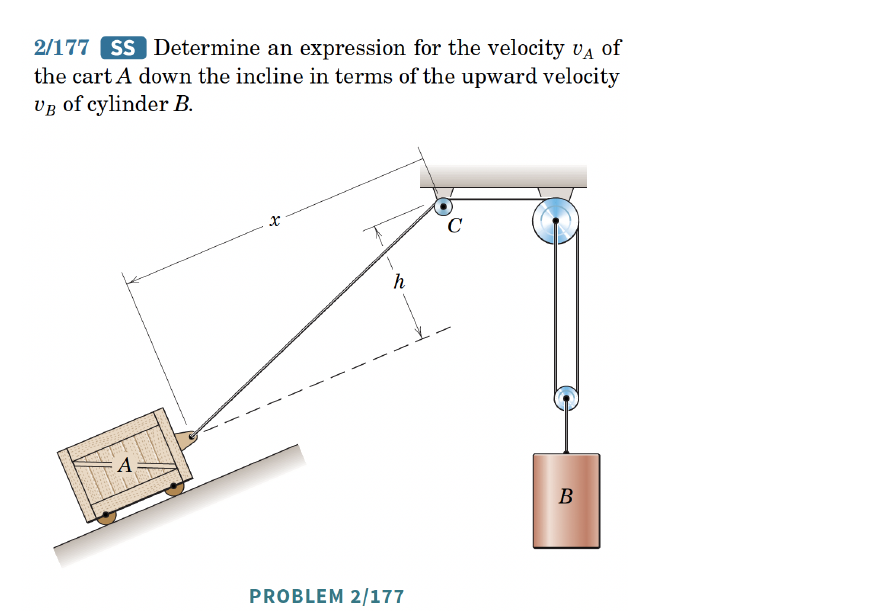
\includegraphics[width=0.5\linewidth,height=\textheight,keepaspectratio]{particle_dynamics/../figures/constrained_motion/02-177.png}

}

\caption{MKB 2/177.}

\end{figure}%

\textbf{6.} {[}MKB 2-179{]}

\begin{figure}[H]

{\centering 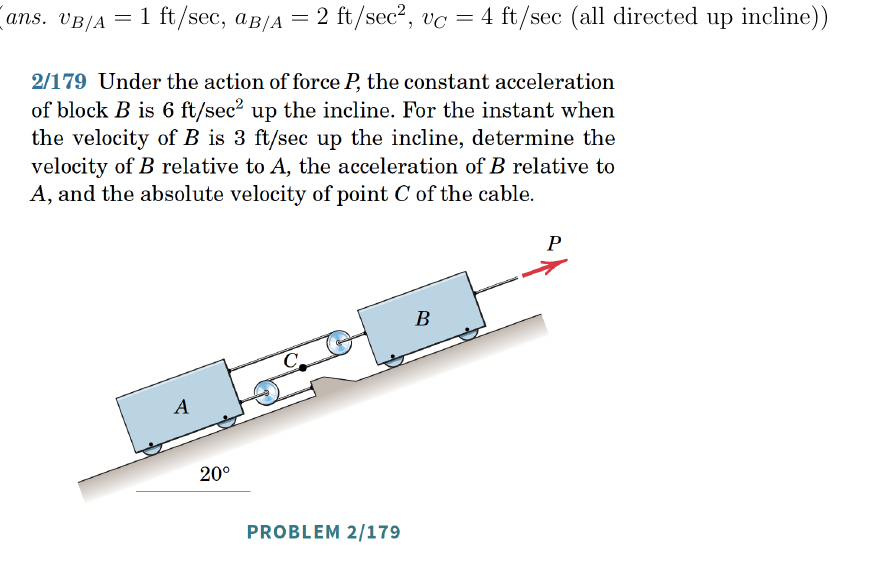
\includegraphics[width=0.5\linewidth,height=\textheight,keepaspectratio]{particle_dynamics/../figures/constrained_motion/02-179.png}

}

\caption{MKB 2/179.}

\end{figure}%

\chapter{The Serret-Frenet Basis}\label{the-serret-frenet-basis}

In general, the path of a particle is a curve in space --- we refer to
such curves as \emph{space curves}.

Consider a fixed curve \(\mathcal{C}\) embedded in \(\mathbb{E}^3\). Let
the position vector of a point \(P\in\mathcal{C}\) be \({\bf r}\). In
Cartesian coordinates, \({\bf r} = x{\bf E}_x+y{\bf E}_y+z{\bf E}_z\).

Recall the arc-length parameter \(s\) associated with \(\mathcal{C}\):
\begin{align*}
    \lp\frac{ds}{dt}\rp^2 = \frac{d{\bf r}}{dt}\cdot\frac{d{\bf r}}{dt} = \frac{dx}{dt}\frac{dx}{dt}+\frac{dy}{dt}\frac{dy}{dt}+\frac{dz}{dt}\frac{dz}{dt}.
\end{align*} This parameter uniquely identifies a point \(P\) on
\(\mathcal{C}\), giving the representation \({\bf r} = \hat{\bf r}(s)\).

\section{The Serret-Frenet Triad}\label{the-serret-frenet-triad}

\begin{center}
\pandocbounded{
\includegraphics[keepaspectratio]{particle_dynamics/serret_frenet_triad_files/figure-pdf/unnamed-chunk-1-1.pdf}}
\end{center}

The Serret-Frenet basis \(\{{\bf e}_t,{\bf e}_n,{\bf e}_b\}\) is defined
at the point \(P\); it depends on the curve and the particle's location
on it.

\begin{tcolorbox}[enhanced jigsaw, arc=.35mm, bottomrule=.15mm, bottomtitle=1mm, breakable, colback=white, colbacktitle=quarto-callout-tip-color!10!white, colframe=quarto-callout-tip-color-frame, coltitle=black, left=2mm, leftrule=.75mm, opacityback=0, opacitybacktitle=0.6, rightrule=.15mm, title=\textcolor{quarto-callout-tip-color}{\faLightbulb}\hspace{0.5em}{Think!}, titlerule=0mm, toprule=.15mm, toptitle=1mm]

\textbf{Question:} How do we define the unit tangent vector?

\begin{quote}
\textbf{Answer}

Recall the unit tangent vector: \begin{align}
    {\bf e}_t = \hat{\bf e}_t(s) = \frac{d{\bf r}}{ds} = \lim_{\Delta s\rightarrow 0}\frac{\hat{\bf r}(s+\Delta s)-\hat{\bf r}(s)}{\Delta s}.
\end{align}

The hat (\(\hat{.}\)) indicates that this function is now expressed in
terms of another variable, \(s\). \({\bf e}_t\) is known as the unit
tangent vector to \(\mathcal{C}\) at the point \(P\).
\end{quote}

\end{tcolorbox}

For general motion, \(||\Delta{\bf r}||\neq ds\) except in the
infinitesimal sense:
\(\hat{\bf r}(s+\Delta s)-\hat{\bf r}(s) \rightarrow \Delta s{\bf e}_t\)
as \(\Delta s\rightarrow 0\) and \(d{\bf r}\) is tangent to the curve.

\begin{center}
\pandocbounded{
\includegraphics[keepaspectratio]{particle_dynamics/serret_frenet_triad_files/figure-pdf/unnamed-chunk-2-1.pdf}}
\end{center}

We need to determine the expression for the acceleration in the
Serret-Frenet basis. \begin{align}
    {\bf a} = \dot{\bf v} = \dot{v}{\bf e}_t+v\dot{\bf e}_t
\end{align} where \begin{align}
    \dot{\bf e}_t = \frac{d\hat{\bf e}_t}{ds}\frac{ds}{dt} = v\frac{d{\bf e}_t}{ds}.
\end{align} The derivative \(\frac{d\hat{\bf e}_t}{ds}\) only depends on
the curve that the particle is tracing.

\begin{tcolorbox}[enhanced jigsaw, arc=.35mm, bottomrule=.15mm, bottomtitle=1mm, breakable, colback=white, colbacktitle=quarto-callout-tip-color!10!white, colframe=quarto-callout-tip-color-frame, coltitle=black, left=2mm, leftrule=.75mm, opacityback=0, opacitybacktitle=0.6, rightrule=.15mm, title=\textcolor{quarto-callout-tip-color}{\faLightbulb}\hspace{0.5em}{Think!}, titlerule=0mm, toprule=.15mm, toptitle=1mm]

\textbf{Question:} What do we know about the direction of
\(\frac{d\hat{\bf e}_t}{ds}\)?

\begin{quote}
\textbf{Answer}

We can show that \({\bf e}_t\) and \(\frac{d\hat{\bf e}_t}{ds}\) are
perpendicular by differentiating \({\bf e}_t\cdot{\bf e}_t = 1\):
\begin{align}
    \frac{d}{ds}\lp{\bf e}_t\cdot{\bf e}_t \rp = {\bf e}_t\cdot\frac{d{\bf e}_t}{ds} = 0.
\end{align}
\end{quote}

\end{tcolorbox}

\begin{tcolorbox}[enhanced jigsaw, arc=.35mm, bottomrule=.15mm, bottomtitle=1mm, breakable, colback=white, colbacktitle=quarto-callout-tip-color!10!white, colframe=quarto-callout-tip-color-frame, coltitle=black, left=2mm, leftrule=.75mm, opacityback=0, opacitybacktitle=0.6, rightrule=.15mm, title=\textcolor{quarto-callout-tip-color}{\faLightbulb}\hspace{0.5em}{Think!}, titlerule=0mm, toprule=.15mm, toptitle=1mm]

\textbf{Question:} What do we know about the magnitude of
\(\frac{d\hat{\bf e}_t}{ds}\)?

\begin{quote}
\textbf{Answer}

Consider two curves. Draw the unit tangent vectors at the same distance
along the curve, \(ds\), apart and draw their difference,
\(\Delta {\bf e}_t\).

\pandocbounded{
\includegraphics[keepaspectratio]{particle_dynamics/serret_frenet_triad_files/figure-pdf/unnamed-chunk-3-1.pdf}}

For which of these two curves is the magnitude of
\(\frac{\Delta \hat{\bf e}_t}{\Delta s}\) higher?

As the curve begins to resemble a line, the magnitude of
\(\frac{d\hat{\bf e}_t}{ds}\) becomes smaller. As the \emph{curvature}
of a curve increases, so does the magnitude of
\(\frac{d\hat{\bf e}_t}{ds}\).
\end{quote}

\end{tcolorbox}

\begin{tcolorbox}[enhanced jigsaw, arc=.35mm, bottomrule=.15mm, bottomtitle=1mm, breakable, colback=white, colbacktitle=quarto-callout-important-color!10!white, colframe=quarto-callout-important-color-frame, coltitle=black, left=2mm, leftrule=.75mm, opacityback=0, opacitybacktitle=0.6, rightrule=.15mm, title=\textcolor{quarto-callout-important-color}{\faExclamation}\hspace{0.5em}{Note! Derivatives of a unit vector}, titlerule=0mm, toprule=.15mm, toptitle=1mm]

It is a common mistake to assume that the derivative of a unit vector is
necessarily a unit vector. Recall:
\(\dot{\bf e}_r = \dot{\theta}{\bf e}_\theta\) is not generally a unit
vector.

\end{tcolorbox}

Hence, we define: \begin{align}
    \kappa{\bf e}_n = \frac{d{\bf e}_t}{ds},
\end{align} where \(\kappa = \lnorm \frac{d{\bf e}_t}{ds}\rnorm \geq 0\)
and \(\lnorm{\bf e}_n\rnorm=1\).

\begin{itemize}
\tightlist
\item
  \({\bf e}_n\) is the unit \textbf{principal normal} vector.
\item
  \(\kappa\) is the \textbf{curvature} of \(\mathcal{C}\) at \(P\).
\item
  The \textbf{radius of curvature} is \(\rho = 1/\kappa\).
\end{itemize}

For any point on a curve, three nearby non-collinear points define the
\textbf{osculating circle} (radius \(\rho\), center of curvature).

\begin{figure}[H]

{\centering \pandocbounded{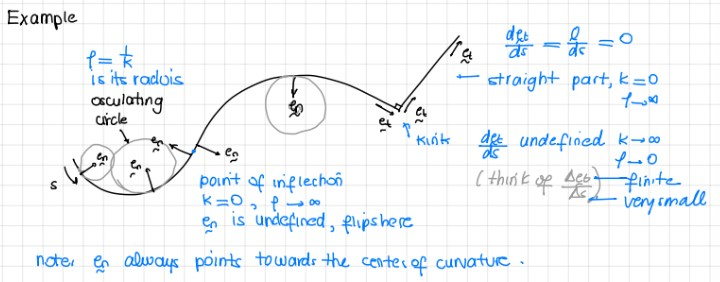
\includegraphics[keepaspectratio]{particle_dynamics/../figures/serret_frenet_triad/serret-frenet-triad-example.jpg}}

}

\caption{Serret-Frenet triad example}

\end{figure}%

\begin{tcolorbox}[enhanced jigsaw, arc=.35mm, bottomrule=.15mm, bottomtitle=1mm, breakable, colback=white, colbacktitle=quarto-callout-tip-color!10!white, colframe=quarto-callout-tip-color-frame, coltitle=black, left=2mm, leftrule=.75mm, opacityback=0, opacitybacktitle=0.6, rightrule=.15mm, title=\textcolor{quarto-callout-tip-color}{\faLightbulb}\hspace{0.5em}{Think!}, titlerule=0mm, toprule=.15mm, toptitle=1mm]

\textbf{Question:} When is \({\bf e}_n\) not uniquely defined?

\begin{quote}
\textbf{Answer}

When \(d{\bf e}_t/ds = {\bf 0}\) (i.e.~\(\kappa = 0\)), such as on a
straight line, at an inflection point, or at a corner. In this case,
\({\bf e}_n\) is defined as any unit vector perpendicular to
\({\bf e}_t\).

Example: In problem 03/040, we choose the Serret-Frenet basis on the
straight portion of the curve to be such that it transitions smoothly to
the curved portion of the curve.
\end{quote}

\end{tcolorbox}

The unit \textbf{binormal} vector: \begin{align*}
    {\bf e}_b = {\bf e}_t\times{\bf e}_n.
\end{align*}

Concluding remarks:

\begin{itemize}
\tightlist
\item
  \(\{{\bf e}_t,{\bf e}_n,{\bf e}_b\}\) is orthonormal and right-handed.
\item
  The \textbf{osculating plane} is spanned by \({\bf e}_t\) and
  \({\bf e}_n\); it contains the osculating circle.
\item
  The \textbf{rectifying plane} is spanned by \({\bf e}_t\) and
  \({\bf e}_b\).
\item
  The \textbf{normal plane} is spanned by \({\bf e}_n\) and
  \({\bf e}_b\).
\end{itemize}

A vector can be expressed in the Serret-Frenet basis as in any other
basis. The Serret-Frenet basis is not a fixed basis. \begin{align}
    {\bf b} = b_t{\bf e}_t+b_n{\bf e}_n = b_x{\bf E}_x+b_y{\bf E}_y+b_z{\bf E}_z.
\end{align}

Check out the following animation showing the osculating circle and
video placing the Serret-Frenet basis on a bobsled.

\url{https://www.youtube.com/watch?v=q2I1oHxPgaQ}

\url{https://www.youtube.com/shorts/NyphZOJggFk?feature=share}

\url{https://www.youtube.com/watch?v=0ACqRREH180}

\url{https://www.youtube.com/watch?v=j2PnkdtIdQ8}

\section{Kinematics}\label{kinematics-1}

Position, velocity, and acceleration in the Serret-Frenet basis:
\begin{align*}
    & {\bf r} = x{\bf E}_x+y{\bf E}_y+z{\bf E}_z = {\bf r}(t) = \hat{{\bf r}(s(t))}.\\
    & {\bf v} = \dot{x}{\bf E}_x+\dot{y}{\bf E}_y+\dot{z}{\bf E}_z = \frac{d{\bf r}}{ds}\frac{ds}{dt} = \frac{ds}{dt}{\bf e}_t = v{\bf e}_t.\\
    & {\bf a} = \dot{\bf v} = \frac{d}{dt}\lp\frac{ds}{dt}{\bf e}_t\rp = \frac{d^2}{dt^2}{\bf e}_t+\frac{ds}{dt}\frac{d{\bf e}_s}{ds} = \frac{d^2}{dt^2}{\bf e}_t+\frac{ds}{dt}\frac{d{\bf e}_t}{ds}\frac{ds}{dt} = \dot{v}{\bf e}_t+\kappa v^2{\bf e}_n.
\end{align*}

\section{Kinetics}\label{kinetics}

\begin{align}
    {\bf F} &= m{\bf a}\\
    F_t{\bf e}_t+F_n{\bf e}_n+F_b{\bf e}_b &= m\lp\dot{v}{\bf e}_t+\kappa v^2{\bf e}_n\rp.
\end{align} Note that forces in the binormal direction should always
balance.

\subsection{Example: Problem 03/040 and Roller Coaster
Design}\label{example-problem-03040-and-roller-coaster-design}

\begin{tcolorbox}[enhanced jigsaw, arc=.35mm, bottomrule=.15mm, bottomtitle=1mm, breakable, colback=white, colbacktitle=quarto-callout-tip-color!10!white, colframe=quarto-callout-tip-color-frame, coltitle=black, left=2mm, leftrule=.75mm, opacityback=0, opacitybacktitle=0.6, rightrule=.15mm, title=\textcolor{quarto-callout-tip-color}{\faLightbulb}\hspace{0.5em}{Think!}, titlerule=0mm, toprule=.15mm, toptitle=1mm]

\textbf{Question:} Consider the design of a roller coaster that is a
circular ring. Comment on its safety.

\begin{quote}
\textbf{Answer}

At the transition between the circular and straight portions, there is a
jump in curvature, hence a jump in acceleration, hence a jump in the
normal force --- producing a jerk. For a circular loop, the normal force
goes from 0 to a finite value instantaneously. This could snap the
rider's neck. Instead, we use two connected \textbf{clothoids} (Euler
spirals), whose curvature is proportional to arc length.
\end{quote}

\end{tcolorbox}

\section{The Serret-Frenet Formulae}\label{the-serret-frenet-formulae}

We want the derivatives of the Serret-Frenet basis vectors with respect
to \(s\).

We already have: \begin{align}
    \frac{d{\bf e}_t}{ds} = \kappa{\bf e}_n.
\end{align}

Since \({\bf e}_b\cdot{\bf e}_b = 1\), we have
\(\frac{d{\bf e}_b}{ds}\cdot{\bf e}_b = 0\).

Also from \({\bf e}_t\cdot{\bf e}_b = 0\), we get
\(\frac{d{\bf e}_b}{ds}\cdot{\bf e}_t=0\). So \(\frac{d{\bf e}_b}{ds}\)
is parallel to \({\bf e}_n\): \begin{align}
    & {\bf e}_t\cdot{\bf e}_b = 0\\
    & \frac{d{\bf e}_t}{ds}\cdot{\bf e}_b+\frac{d{\bf e}_b}{ds}\cdot{\bf e}_t = 0\\
    & \kappa{\bf e}_n\cdot{\bf e}_b+\frac{d{\bf e}_b}{ds}\cdot{\bf e}_t = 0\\
    & \frac{d{\bf e}_b}{ds}\cdot{\bf e}_t=0.
\end{align} Consequently, we define \begin{align}
    \frac{d{\bf e}_b}{ds} = -\tau{\bf e}_n,
\end{align} where \(\tau\) is the \textbf{torsion} of \(\mathcal{C}\) at
\(P\). The negative sign in the above formula is a convention.

Then: \begin{align}
    \frac{d{\bf e}_n}{ds} &= \frac{d}{ds}\lp{\bf e}_b\times{\bf e}_t\rp\\
    &= \frac{d{\bf e}_b}{ds}\times{\bf e}_t+{\bf e}_b\times\frac{d{\bf e}_t}{ds}\\
    &= (-\tau{\bf e}_n)\times{\bf e}_t+{\bf e}_b\times\kappa{\bf e}_n\\
    &= -\kappa{\bf e}_t+\tau{\bf e}_b.
\end{align}

In summary (the Serret-Frenet formulae): \begin{align}
    \begin{bmatrix}
        \frac{d{\bf e}_t}{ds}\\
        \frac{d{\bf e}_n}{ds}\\
        \frac{d{\bf e}_b}{ds}
    \end{bmatrix}
    =
    \begin{bmatrix}
        0 & \kappa & 0\\
        -\kappa & 0 & \tau\\
        0 & -\tau & 0
    \end{bmatrix}
    \begin{bmatrix}
        {\bf e}_t\\
        {\bf e}_n\\
        {\bf e}_b
    \end{bmatrix}.
\end{align}

Define the \textbf{Darboux vector}
\(\bomega_{SF} = \kappa{\bf e}_b+\tau{\bf e}_t\) so that: \begin{align}
    \frac{d{\bf e}_i}{ds} = \bomega_{SF}\times{\bf e}_i, \quad i = t, n, b.
\end{align}

\url{https://youtu.be/OB13c0WlUSg}

\subsection{Example: A Particle on a
Helix}\label{example-a-particle-on-a-helix}

For a helix \(x=R\cos(\theta)\), \(y=R\sin(\theta)\),
\(z=\alpha R\theta\): \begin{align}
    {\bf r} = R{\bf e}_r+\alpha R\theta{\bf E}_z = x{\bf E}_x+y{\bf E}_y+z{\bf E}_z.
\end{align} \begin{align}
    \kappa = \frac{1}{R(1+\alpha^2)}, \qquad \tau = \frac{\alpha}{(1+\alpha^2)R}.
\end{align}

\section{The Curvature Formula for a Plane
Curve}\label{the-curvature-formula-for-a-plane-curve}

Consider a point \(P\) tracing a plane curve with \(y = f(x)\),
\(z = z_0\), so that \begin{align}
    {\bf r} = x{\bf E}_x+f(x){\bf E}_y+z_0{\bf E}_z.
\end{align}

Determining the arc-length parameter \(s\): \begin{align}
    \begin{split}
        & \frac{d{\bf r}}{dt} = \frac{dx}{dt}{\bf E}_x+\frac{df}{dx}\frac{dx}{dt}{\bf E}_y,\\
        & \lp\frac{ds}{dt}\rp^2 = \lp 1+\lp\frac{df}{dx}\rp^2\rp\lp\frac{dx}{dt}\rp^2,\\
        & \frac{ds}{dt} = \frac{dx}{dt}\sqrt{1+\lp\frac{df}{dx}\rp^2},\\
        & s = s(x) = \int_{x_0}^x\sqrt{1+\lp\frac{df}{du}\rp^2}\,du+s(x_0).
    \end{split}
\end{align}

The tangent vector: \begin{align}
    {\bf e}_t = \frac{d{\bf r}}{ds} = \frac{d{\bf r}}{dx}\frac{dx}{ds} = \frac{1}{\sqrt{1+\lp\frac{df}{dx}\rp^2}}\lp{\bf E}_x+\frac{df}{dx}{\bf E}_y\rp.
\end{align}

The \(\kappa{\bf e}_n\) expression: \begin{align}
    \kappa{\bf e}_n = \frac{d{\bf e}_t}{ds} = \frac{d{\bf e}_t}{dx}\frac{dx}{ds} = \frac{\frac{d^2 f}{dx^2}}{\lp1+\lp \frac{df}{dx}\rp^2\rp^2}\lp{\bf E}_y-\frac{df}{dx}{\bf E}_x\rp.
\end{align}

Recalling that \({\bf e}_n\) is a unit vector and \(\kappa \geq 0\):
\begin{align}
    \begin{split}
        & \kappa = \kappa(x) = \frac{\left|\frac{d^2 f}{dx^2}\right|}{\lp\sqrt{1+\lp\frac{df}{dx}\rp^2}\rp^3},\\
        & {\bf e}_n = \frac{\text{sgn}\lp\frac{d^2 f}{dx^2}\rp}{\sqrt{1+\lp\frac{df}{dx}\rp^2}}\lp{\bf E}_y-\frac{df}{dx}{\bf E}_x\rp,
    \end{split}
\end{align} where \(\text{sgn}(a)=1\) if \(a>0\) and \(-1\) if \(a<0\).

The binormal vector and torsion: \begin{align}
    {\bf e}_b = {\bf e}_t\times{\bf e}_n = \text{sgn}\lp\frac{d^2 f}{dx^2}\rp{\bf E}_z,
\end{align} and because this vector is piecewise constant, the torsion
of the plane curve is \(\tau = 0\).

\section{Alternative Notation for Plane
Curves}\label{alternative-notation-for-plane-curves}

\emph{This section is not usually covered.}

For plane curves, some texts define the angle \(\beta = \beta(s)\) such
that: \begin{align}
    {\bf e}_t = \cos(\beta){\bf E}_x+\sin(\beta){\bf E}_y, \qquad \bar{\bf e}_n = \cos(\beta){\bf E}_y-\sin(\beta){\bf E}_x.
\end{align} Then \(\kappa = \left|\frac{d\beta}{ds}\right|\) and
\(\frac{d\beta}{ds}\) is the rate of rotation of the triad about
\({\bf E}_z\).

\section{Summary}\label{summary-5}

\textbf{Serret--Frenet basis}
\(\{\mathbf{e}_t,\mathbf{e}_n,\mathbf{e}_b\}\): \begin{align}
    \mathbf{v} &= v\,\mathbf{e}_t, \qquad
    \mathbf{a} = \dot v\,\mathbf{e}_t + \kappa v^2\,\mathbf{e}_n, \qquad
    \mathbf{e}_b = \mathbf{e}_t\times\mathbf{e}_n.
\end{align} The curvature is \(\kappa=1/\rho\) (radius of curvature
\(\rho\)). The BoLM gives \(F_t = m\dot v\) and \(F_n = m\kappa v^2\).

\section{Exercises}\label{exercises-7}

\emph{The following problems are from Set 07 -- The Serret--Frenet
Basis.}

\textbf{1.} {[}MKB 2/079{]} Analyse the acceleration vector in the
Serret--Frenet basis.

\begin{figure}[H]

{\centering 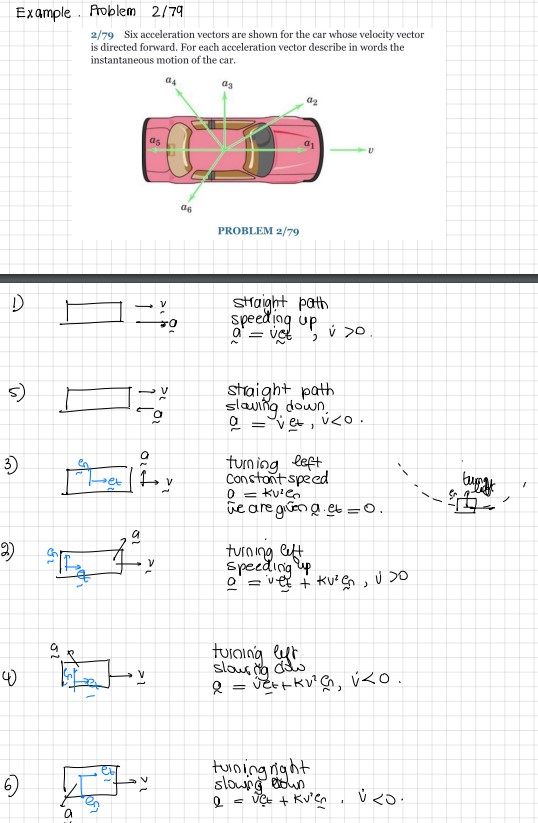
\includegraphics[width=0.5\linewidth,height=\textheight,keepaspectratio]{particle_dynamics/../figures/serret_frenet_triad/02-079.jpg}

}

\caption{MKB 2/079.}

\end{figure}%

\textbf{2.} {[}MKB 02-090{]} Note that \(\dot v \neq \|\mathbf{a}\|\);
acceleration has both tangential and normal components. \emph{(ans.
\(v = 20\) m/s)}

\begin{figure}[H]

{\centering 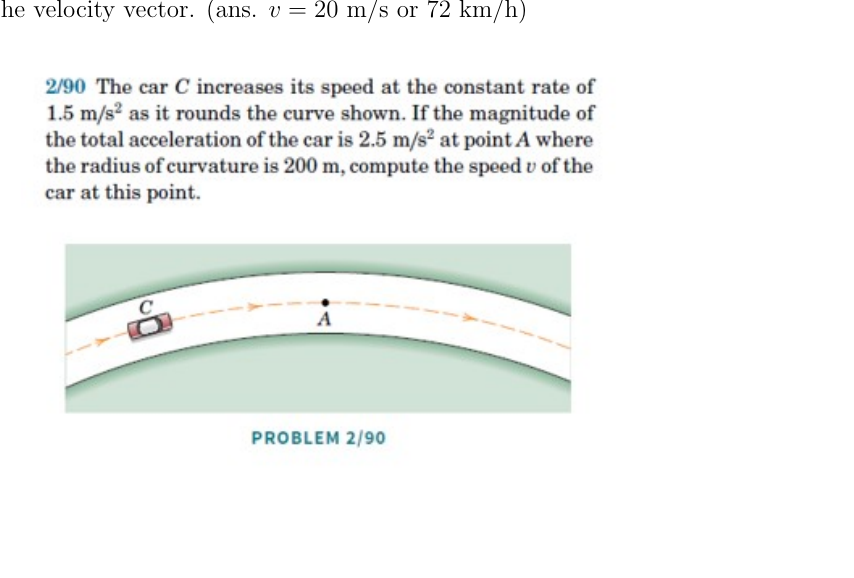
\includegraphics[width=0.5\linewidth,height=\textheight,keepaspectratio]{particle_dynamics/../figures/serret_frenet_triad/02-090.png}

}

\caption{MKB 02-090.}

\end{figure}%

\textbf{3.} {[}MKB 02-091{]} \emph{(ans. \(\rho = 1709\) m)}

\begin{figure}[H]

{\centering 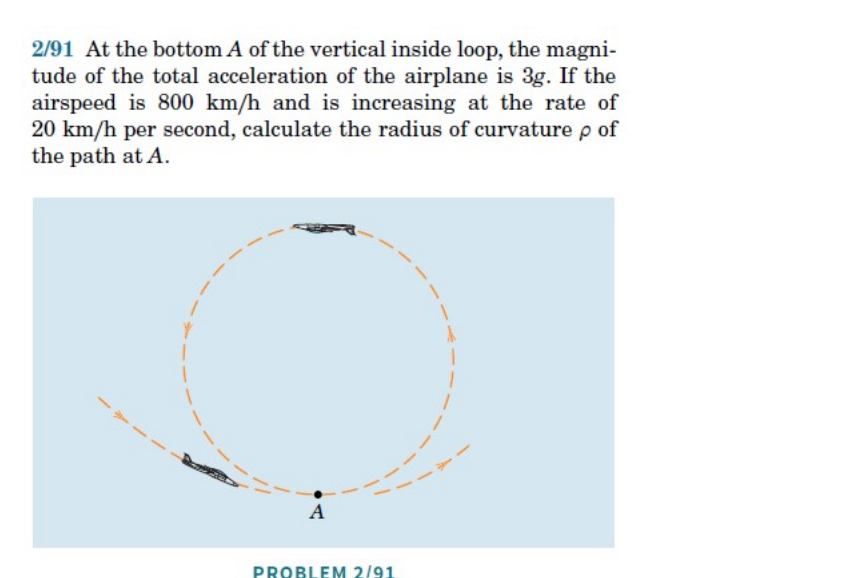
\includegraphics[width=0.5\linewidth,height=\textheight,keepaspectratio]{particle_dynamics/../figures/serret_frenet_triad/02-091.png}

}

\caption{MKB 02-091.}

\end{figure}%

\textbf{4.} {[}02-097{]} Follow the 4 steps; express \(\mathbf{e}_t\)
and \(\mathbf{e}_n\) in the Cartesian basis. \emph{(ans. at \(t=1\) s:
\(\dot v=-6.58\) ft/s\(^2\), \(\rho=142.2\) ft; at \(t=2\) s:
\(\dot v=8.75\) ft/s\(^2\), \(\rho=149.7\) ft)}

\begin{figure}[H]

{\centering 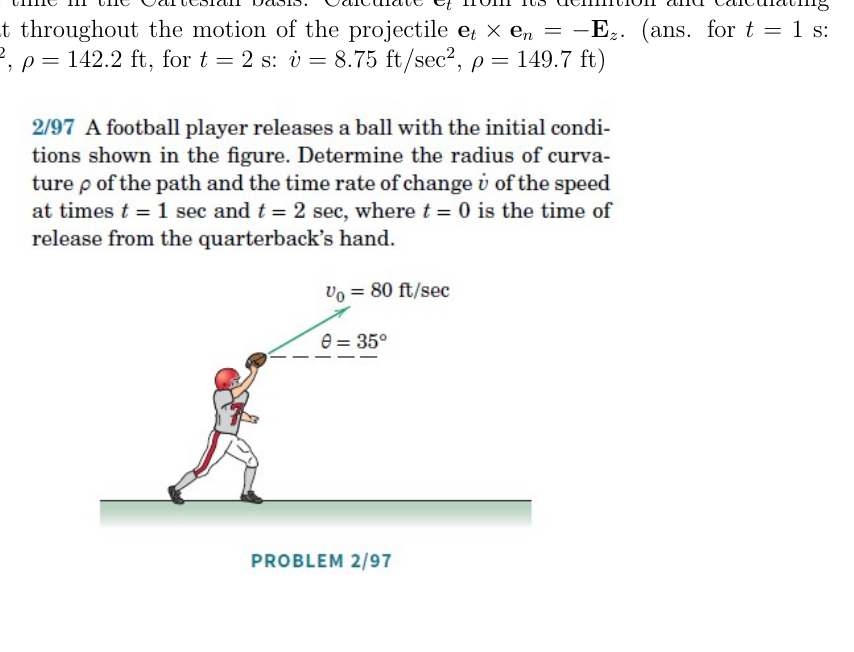
\includegraphics[width=0.5\linewidth,height=\textheight,keepaspectratio]{particle_dynamics/../figures/serret_frenet_triad/02-097.png}

}

\caption{MKB 02-097.}

\end{figure}%

\textbf{5.} {[}02-103{]} \emph{(ans. \((x_C,y_C)=(22.5,-22.9)\) m)}

\textbf{6.} {[}02-199{]} Draw \(\mathbf{e}_t\) and \(\mathbf{e}_n\)
first. \emph{(ans. \(\dot r=15\) m/s, \(\dot\theta=0.325\) rad/s,
\(\rho=129.9\) m)}

\begin{figure}[H]

{\centering 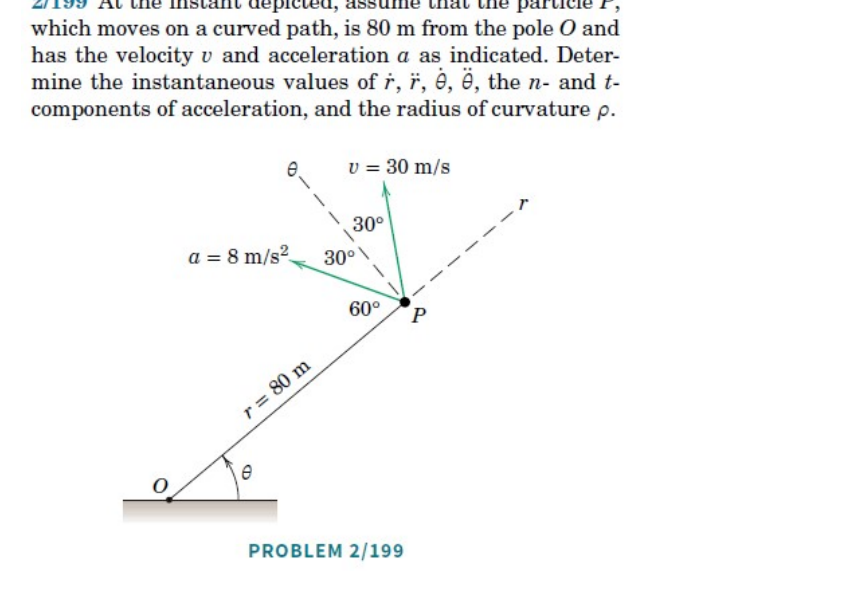
\includegraphics[width=0.5\linewidth,height=\textheight,keepaspectratio]{particle_dynamics/../figures/serret_frenet_triad/02-199.png}

}

\caption{MKB 02-199.}

\end{figure}%

\textbf{7.} {[}03-040{]} Note the jump in normal force at the transition
from straight to curved path. \emph{(ans. (a) \(R=1.177\) N; (b)
\(R=1.664\) N)}

\begin{figure}[H]

{\centering 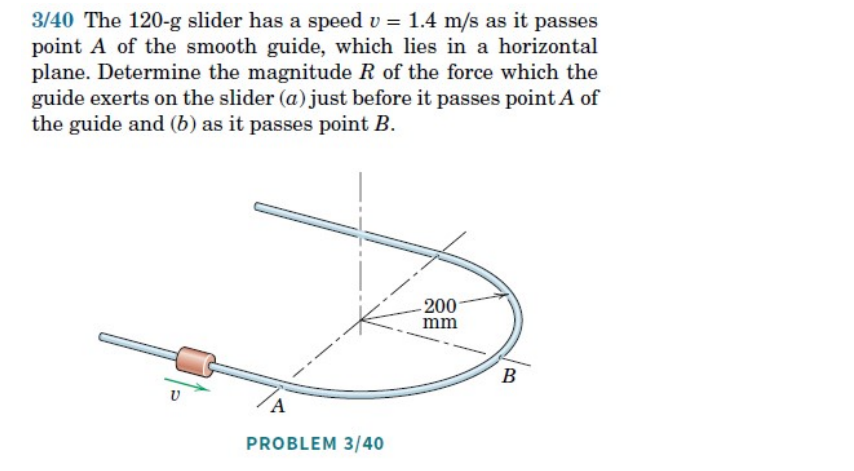
\includegraphics[width=0.5\linewidth,height=\textheight,keepaspectratio]{particle_dynamics/../figures/serret_frenet_triad/03-040.png}

}

\caption{MKB 03-040.}

\end{figure}%

\textbf{8.} {[}03-041{]} What does ``weightless'' mean? \emph{(ans.
\(\rho=24\,000\) ft)}

\begin{figure}[H]

{\centering 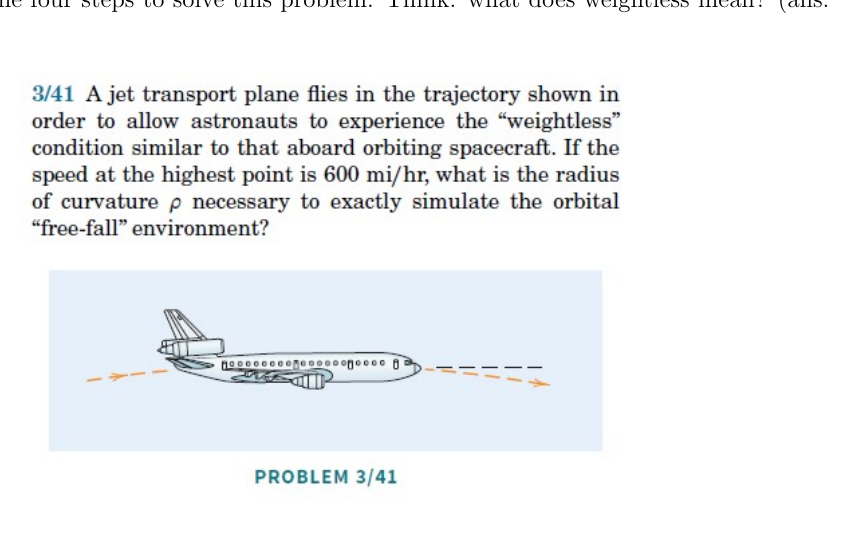
\includegraphics[width=0.5\linewidth,height=\textheight,keepaspectratio]{particle_dynamics/../figures/serret_frenet_triad/03-041.png}

}

\caption{MKB 03-041.}

\end{figure}%

\textbf{9.} {[}03-043{]} Draw the Serret--Frenet basis carefully; the
figure hints at the direction of \(\mathbf{e}_n\). \emph{(ans.
\(v=29.1\) m/s, \(N=12.36\) kN)}

\begin{figure}[H]

{\centering 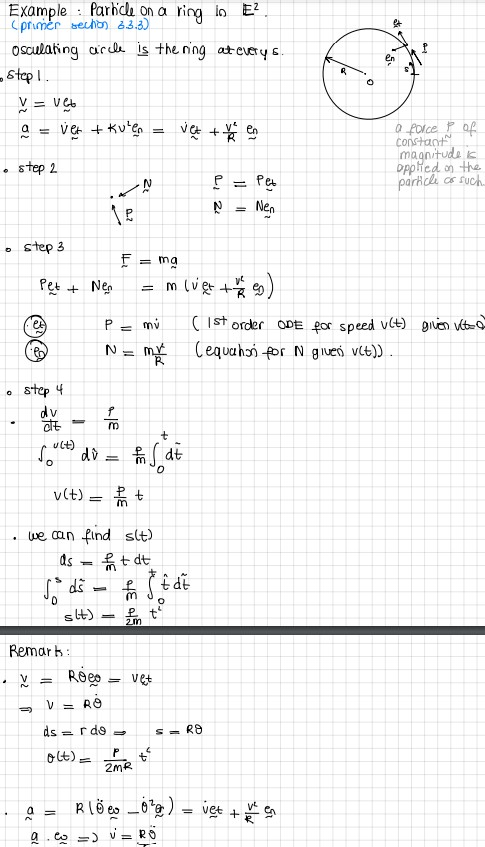
\includegraphics[width=0.5\linewidth,height=\textheight,keepaspectratio]{particle_dynamics/../figures/serret_frenet_triad/eg-particle-on-ring.jpg}

}

\caption{Problem 03/043.}

\end{figure}%

\textbf{10.} {[}OOR 3.1{]}

\begin{figure}[H]

{\centering 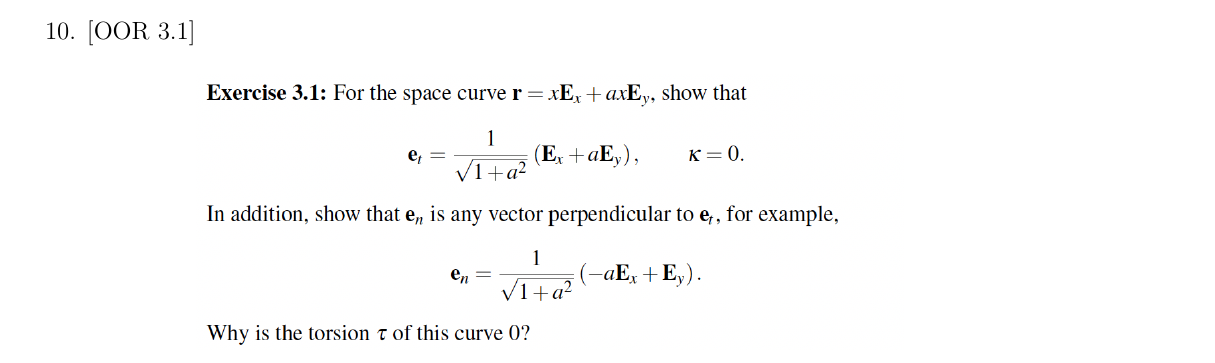
\includegraphics[width=0.7\linewidth,height=\textheight,keepaspectratio]{particle_dynamics/../figures/serret_frenet_triad/oor_3_1.png}

}

\caption{O'Reilly Primer, Exercise 3.1.}

\end{figure}%

\textbf{11.} {[}OOR 3.2{]}

\begin{figure}[H]

{\centering 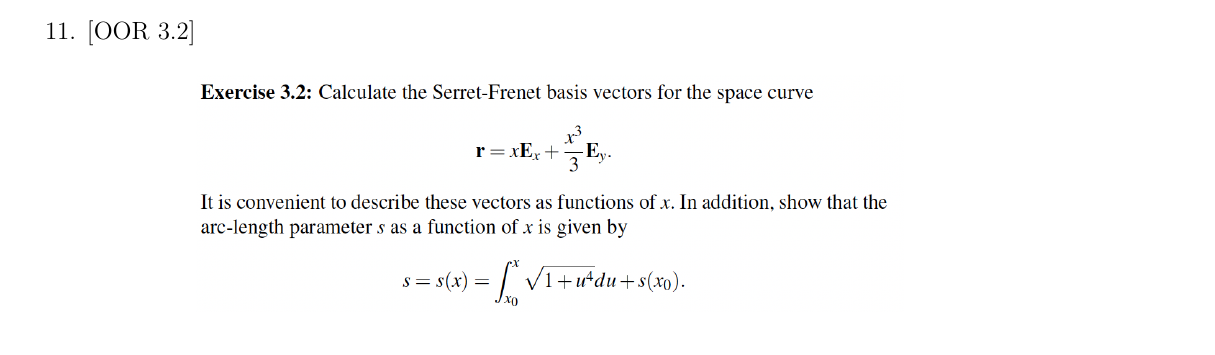
\includegraphics[width=0.7\linewidth,height=\textheight,keepaspectratio]{particle_dynamics/../figures/serret_frenet_triad/oor_3_2.png}

}

\caption{O'Reilly Primer, Exercise 3.2.}

\end{figure}%

\chapter{Spring Force}\label{spring-force}

\section{Introduction}\label{introduction}

\begin{tcolorbox}[enhanced jigsaw, arc=.35mm, bottomrule=.15mm, bottomtitle=1mm, breakable, colback=white, colbacktitle=quarto-callout-tip-color!10!white, colframe=quarto-callout-tip-color-frame, coltitle=black, left=2mm, leftrule=.75mm, opacityback=0, opacitybacktitle=0.6, rightrule=.15mm, title=\textcolor{quarto-callout-tip-color}{\faLightbulb}\hspace{0.5em}{Think!}, titlerule=0mm, toprule=.15mm, toptitle=1mm]

\textbf{Question:} What does it mean for a spring to be linear?

\begin{quote}
\textbf{Answer}

Consider a mass \(m\) suspended by a spring causing an extension
\(\delta\). Suspending a mass \(2m\) causes double the extension,
\(2\delta\).
\end{quote}

\end{tcolorbox}

\textbf{Hooke's Law:} The force generated by a spring is assumed to be
linearly proportional to its extension/compression.

\section{The Simple Harmonic
Oscillator}\label{the-simple-harmonic-oscillator}

Consider a block of mass \(m\) attached to a linear spring of stiffness
\(k\) and unstretched length \(\ell_0\). Denote the current length by
\(\ell\) and the stretch by \(\varepsilon = \ell-\ell_0\).

\begin{center}
\pandocbounded{
\includegraphics[keepaspectratio]{particle_dynamics/spring_force_files/figure-pdf/unnamed-chunk-1-1.pdf}}
\end{center}

\begin{tcolorbox}[enhanced jigsaw, arc=.35mm, bottomrule=.15mm, bottomtitle=1mm, breakable, colback=white, colbacktitle=quarto-callout-tip-color!10!white, colframe=quarto-callout-tip-color-frame, coltitle=black, left=2mm, leftrule=.75mm, opacityback=0, opacitybacktitle=0.6, rightrule=.15mm, title=\textcolor{quarto-callout-tip-color}{\faLightbulb}\hspace{0.5em}{Think!}, titlerule=0mm, toprule=.15mm, toptitle=1mm]

\textbf{Question:} What is the stretch in each case? What is the spring
force?

\begin{quote}
\textbf{Answer}

\begin{enumerate}
\def\labelenumi{(\alph{enumi})}
\item
  Unstretched: Its current length is \(\ell_0\) and its stretch is
  \(\varepsilon =0\).
\item
  Extended: Its current length is \(\ell\) and its stretch is
  \(\varepsilon = \ell-\ell_0>0\). The spring force is
  \({\bf F}_s = -k\varepsilon{\bf E}_x\) pointing to the left.
\item
  Compressed: Its current length is \(\ell\) and its stretch is
  \(\varepsilon = \ell-\ell_0<0\). The spring force is
  \({\bf F}_s = -k\varepsilon{\bf E}_x\) pointing to the right.
\end{enumerate}
\end{quote}

\end{tcolorbox}

\begin{tcolorbox}[enhanced jigsaw, arc=.35mm, bottomrule=.15mm, bottomtitle=1mm, breakable, colback=white, colbacktitle=quarto-callout-important-color!10!white, colframe=quarto-callout-important-color-frame, coltitle=black, left=2mm, leftrule=.75mm, opacityback=0, opacitybacktitle=0.6, rightrule=.15mm, title=\textcolor{quarto-callout-important-color}{\faExclamation}\hspace{0.5em}{Note! Prescribing the spring force}, titlerule=0mm, toprule=.15mm, toptitle=1mm]

The spring force always seeks to return the particle to the unstretched
state. The same expression applies whether the spring is extended or
compressed.

\end{tcolorbox}

\url{https://youtu.be/WtTDHW2JUVY}

\section{Formalism}\label{formalism}

In general:

\begin{figure}[H]

{\centering 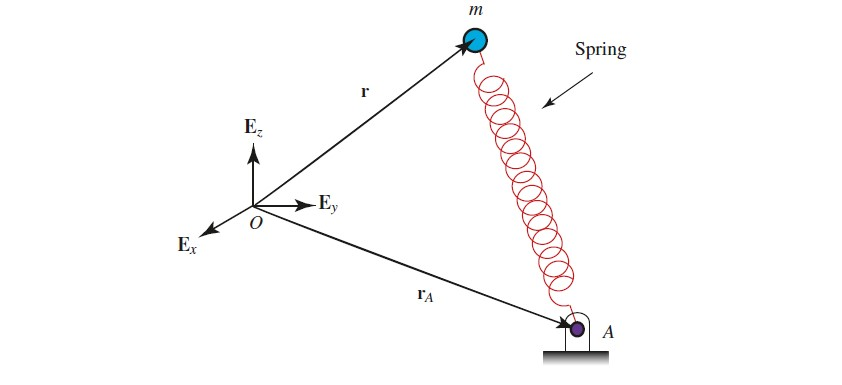
\includegraphics[width=0.5\linewidth,height=\textheight,keepaspectratio]{particle_dynamics/../figures/spring_force/general-spring.jpg}

}

\caption{General spring configuration}

\end{figure}%

\begin{tcolorbox}[enhanced jigsaw, arc=.35mm, bottomrule=.15mm, bottomtitle=1mm, breakable, colback=white, colbacktitle=quarto-callout-tip-color!10!white, colframe=quarto-callout-tip-color-frame, coltitle=black, left=2mm, leftrule=.75mm, opacityback=0, opacitybacktitle=0.6, rightrule=.15mm, title=\textcolor{quarto-callout-tip-color}{\faLightbulb}\hspace{0.5em}{Think!}, titlerule=0mm, toprule=.15mm, toptitle=1mm]

\textbf{Question:} What is the prescription of the spring force in this
general case?

\begin{quote}
\textbf{Answer}

\ldots{}
\end{quote}

\end{tcolorbox}

The stretch is: \begin{align}
    \varepsilon = \lnorm{\bf r}-{\bf r}_A\rnorm-\ell_0,
\end{align} where \(\ell_0\) is the unstretched length. The magnitude
the friction force \({\bf F}_s\) is a statement of Hooke's law.
\begin{align}
    \lnorm{\bf F}_s\rnorm = |K\lp\lnorm{\bf r}-{\bf r}_A\rnorm-\ell_0\rp|.
\end{align} The spring force is: \begin{align}
    {\bf F}_s = -K\lp\lnorm{\bf r}-{\bf r}_A\rnorm-\ell_0\rp\frac{{\bf r}-{\bf r}_A}{\lnorm{\bf r}-{\bf r}_A\rnorm}.
\end{align} This direction is correct in both tension and compression.

\url{https://youtu.be/YiOZregJx9w}

\section{Choosing the Origin}\label{choosing-the-origin}

\subsection{Horizontal Simple Harmonic
Oscillator}\label{horizontal-simple-harmonic-oscillator}

\begin{tcolorbox}[enhanced jigsaw, arc=.35mm, bottomrule=.15mm, bottomtitle=1mm, breakable, colback=white, colbacktitle=quarto-callout-tip-color!10!white, colframe=quarto-callout-tip-color-frame, coltitle=black, left=2mm, leftrule=.75mm, opacityback=0, opacitybacktitle=0.6, rightrule=.15mm, title=\textcolor{quarto-callout-tip-color}{\faLightbulb}\hspace{0.5em}{Think!}, titlerule=0mm, toprule=.15mm, toptitle=1mm]

\textbf{Question:} Derive the equations of motion of the harmonic
oscillator with the origin at the free end of the spring when it is
unstretched.

\begin{quote}
\textbf{Answer}

The equation of motion is \begin{align}
    \ddot{x}+\frac{k}{m}x = 0,
\end{align} where \(x\) is measured from the undeformed position.
\end{quote}

\end{tcolorbox}

\begin{tcolorbox}[enhanced jigsaw, arc=.35mm, bottomrule=.15mm, bottomtitle=1mm, breakable, colback=white, colbacktitle=quarto-callout-tip-color!10!white, colframe=quarto-callout-tip-color-frame, coltitle=black, left=2mm, leftrule=.75mm, opacityback=0, opacitybacktitle=0.6, rightrule=.15mm, title=\textcolor{quarto-callout-tip-color}{\faLightbulb}\hspace{0.5em}{Think!}, titlerule=0mm, toprule=.15mm, toptitle=1mm]

\textbf{Question:} Derive the equations of motion with the origin at the
fixed end of the spring.

\begin{quote}
\textbf{Answer}

\ldots{}
\end{quote}

\end{tcolorbox}

\subsection{Vertical Simple Harmonic
Oscillator}\label{vertical-simple-harmonic-oscillator}

By analogy, the equation of motion of a vertical harmonic oscillator is:
\begin{align}
    \ddot{x}+\frac{k}{m}x = 0,
\end{align} where \(x\) is measured from the \textbf{static equilibrium}
position.

\url{https://www.youtube.com/watch?v=YE9N2f2qTqg}

\section{Summary}\label{summary-6}

The spring force on a mass \(m\) at position \(\mathbf{r}\), attached to
a spring (stiffness \(K\), unstretched length \(\ell_0\)) with base at
\(\mathbf{r}_A\): \begin{align}
    \mathbf{F}_s = -K(\|\mathbf{r}-\mathbf{r}_A\|-\ell_0)\,\frac{\mathbf{r}-\mathbf{r}_A}{\|\mathbf{r}-\mathbf{r}_A\|}.
\end{align}

\section{Exercises}\label{exercises-8}

Complete
\href{https://colab.research.google.com/drive/1zIuB6Ovq1QWNSRoEht7LhWr2APq-lmqb?usp=sharing}{this}
introduction to vibrations.

\emph{The following problems are from Set 09 -- Spring Force (Chapter 8
of MKB). In each problem, find the equation of motion of the block.}

\textbf{1.} {[}08-002{]} \emph{(ans. \(\omega_n = 12\) rad/s,
\(f_n = 1.910\) Hz)}

\begin{figure}[H]

{\centering 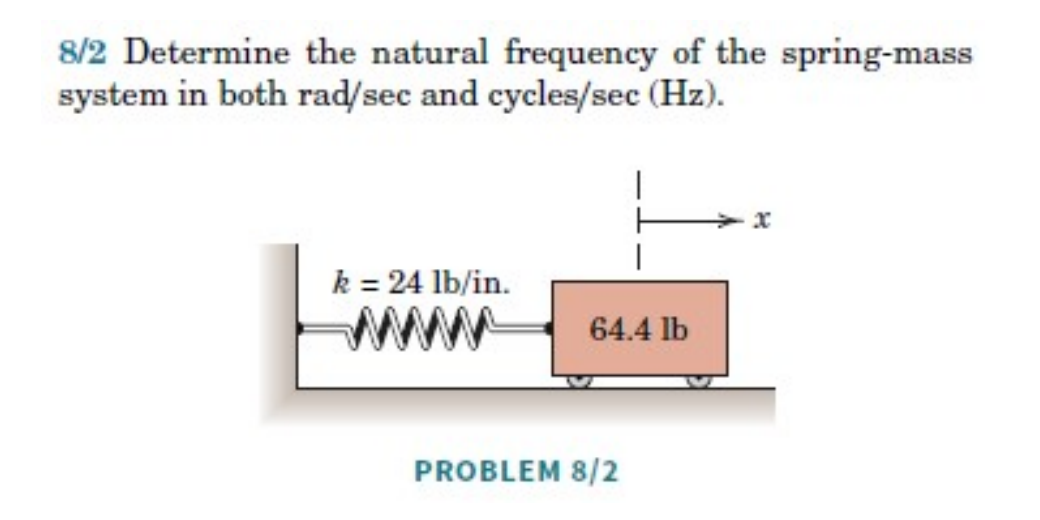
\includegraphics[width=0.5\linewidth,height=\textheight,keepaspectratio]{particle_dynamics/../figures/spring_force/08-002.png}

}

\caption{MKB 08-002.}

\end{figure}%

\textbf{2.} {[}08-004{]} First determine the static deflection of the
spring; take the origin at the statically deflected position.
\emph{(ans. \(\delta_{st} = 0.200\) m, \(\tau = 0.898\) s,
\(v_{\max} = 0.7\) m/s)}

\begin{figure}[H]

{\centering 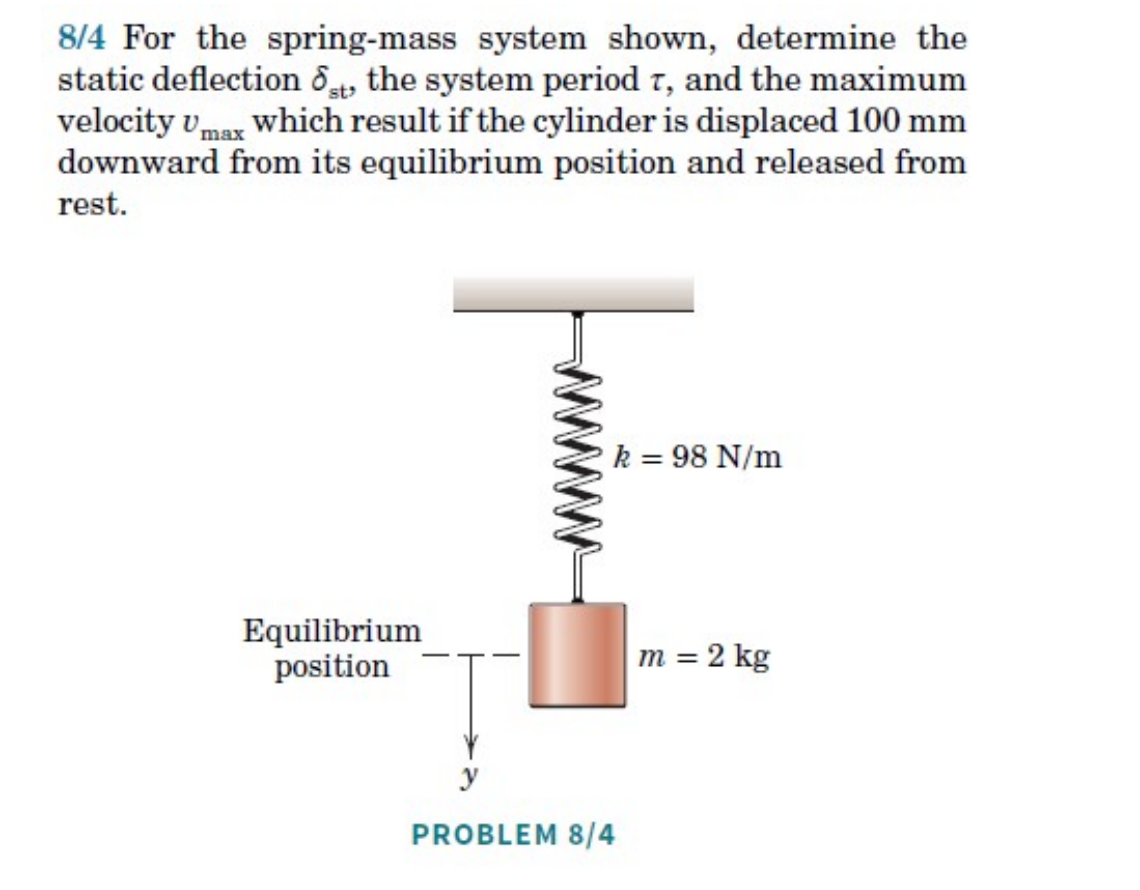
\includegraphics[width=0.5\linewidth,height=\textheight,keepaspectratio]{particle_dynamics/../figures/spring_force/08-004.png}

}

\caption{MKB 08-004.}

\end{figure}%

\url{https://youtu.be/YE9N2f2qTqg}

\textbf{3.} {[}08-019{]} \emph{(ans.
\(\ddot y + \frac{3k}{mL^2}y = 0\))}

\begin{figure}[H]

{\centering 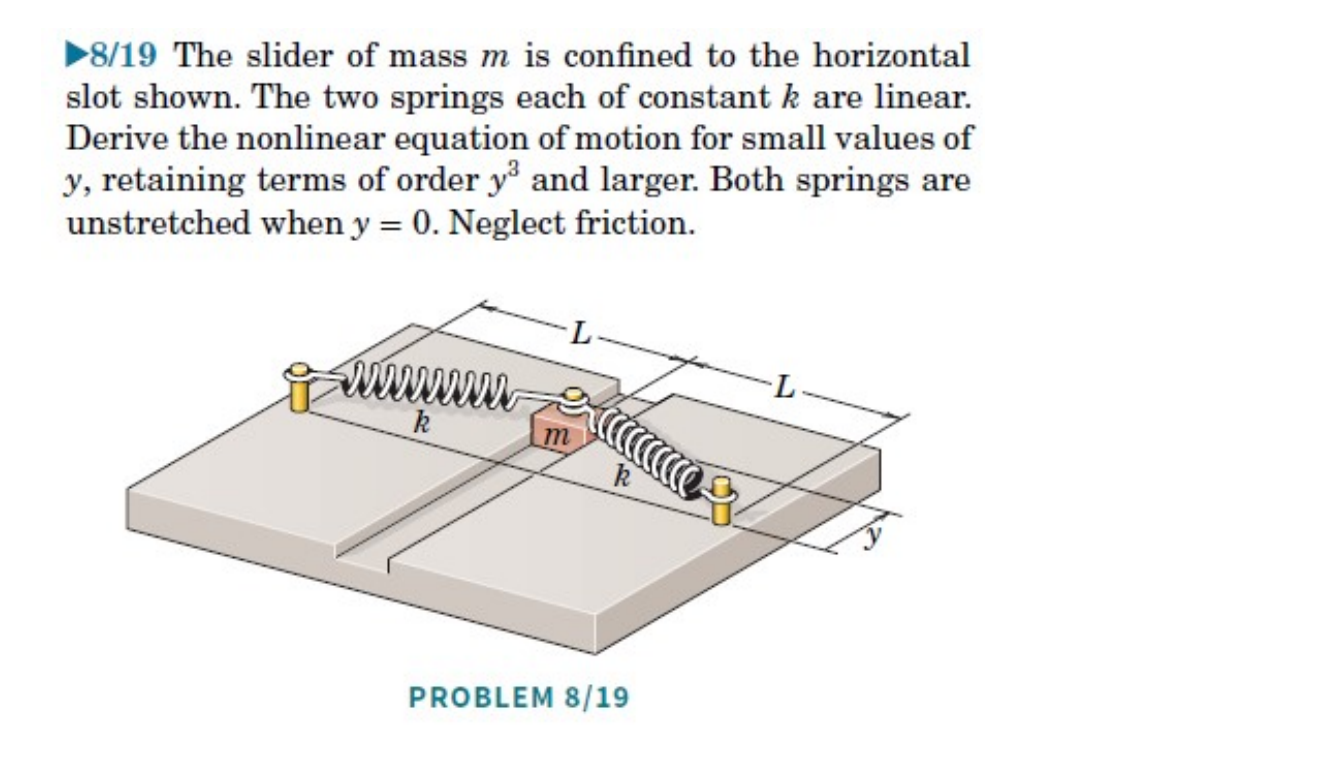
\includegraphics[width=0.5\linewidth,height=\textheight,keepaspectratio]{particle_dynamics/../figures/spring_force/08-019.png}

}

\caption{MKB 08-019.}

\end{figure}%

\chapter{Friction Force}\label{friction-force}

Most theories of friction arise from studies by the French scientist
Charles Augustin de Coulomb (1736--1806).

\section{Introduction}\label{introduction-1}

Consider a block on a rough horizontal surface pushed with force
\({\bf P} = P{\bf E}_x\).

\begin{center}
\pandocbounded{
\includegraphics[keepaspectratio]{particle_dynamics/friction_force_files/figure-pdf/unnamed-chunk-1-1.pdf}}
\end{center}

Upon increasing \(P\), we observe:

\begin{itemize}
\tightlist
\item
  For small \(P\), the block remains at rest.
\item
  Beyond a critical value \(P = P^*\), the block starts to move.
\item
  Once in motion, a constant value \(P = P^{**}\) is required to
  maintain constant speed.
\item
  Both \(P^*\) and \(P^{**}\) are proportional to the normal force
  \(\lnorm{\bf N}\rnorm\).
\end{itemize}

\section{Formalism: Coulomb's Theory of
Friction}\label{formalism-coulombs-theory-of-friction}

We distinguish two types of friction: static and kinetic.

\subsection{Static Friction}\label{static-friction}

When the relative velocity between two surfacesis zero
(\({\bf v}_{rel} = {\bf 0}\)), the friction force \({\bf F}_f\) is
\textbf{unknown} and lies along the contact surface. We must solve for
both its magnitude and direction. We say the static friction force
points in the direction that \textbf{impedes motion}.

\begin{tcolorbox}[enhanced jigsaw, arc=.35mm, bottomrule=.15mm, bottomtitle=1mm, breakable, colback=white, colbacktitle=quarto-callout-tip-color!10!white, colframe=quarto-callout-tip-color-frame, coltitle=black, left=2mm, leftrule=.75mm, opacityback=0, opacitybacktitle=0.6, rightrule=.15mm, title=\textcolor{quarto-callout-tip-color}{\faLightbulb}\hspace{0.5em}{Think!}, titlerule=0mm, toprule=.15mm, toptitle=1mm]

\textbf{Question:} Consider a block on a rough inclined surface that is
not moving. Draw the FBD and write the equation of motion. Do you have
as many equations as unknowns?

\begin{quote}
\textbf{Answer}

Yes. The friction and normal forces have unknown magnitudes, but the
block's acceleration is known (it matches the surface acceleration).
There are as many equations as unknowns.
\end{quote}

\end{tcolorbox}

The magnitude of the static friction force satisfies the \textbf{static
friction criterion}: \begin{align}
    \lnorm{\bf F}_f\rnorm \leq \mu_s\lnorm{\bf N}\rnorm,
\end{align} where \(\mu_s\) is the static friction coefficient.

\subsection{Kinetic Friction}\label{kinetic-friction}

When two bodies are in relative motion (\({\bf v}_{rel} \neq {\bf 0}\)),
the friction force is \textbf{known} (both in magnitude and direction):
\begin{align}
    {\bf F}_f = \mu_k\lnorm{\bf N}\rnorm\lp-\frac{{\bf v}_{rel}}{\lnorm{\bf v}_{rel}\rnorm}\rp,
\end{align} where \(\mu_k\) is the kinetic friction coefficient. This
prescription is used to solve for the motion of the system.

Remarks:

\begin{itemize}
\tightlist
\item
  \(\mu_k\) is also written \(\mu_d\) (dynamic friction coefficient).
\item
  Kinetic friction is a prescription, not a constraint force.
\item
  The magnitude of kinetic friction does not depend on speed.
\end{itemize}

\url{https://youtu.be/_fvCFtpL3c8}

\subsection{Example: Crate Pushed with Incremental
Force}\label{example-crate-pushed-with-incremental-force}

Consider a block on a rough horizontal surface pushed with force
\({\bf P} = P{\bf E}_x\). At \(t=0\), the block is initially at rest and
\(P=0\), then \(P\) is increased linearly.

\begin{center}
\pandocbounded{
\includegraphics[keepaspectratio]{particle_dynamics/friction_force_files/figure-pdf/unnamed-chunk-2-1.pdf}}
\end{center}

\begin{enumerate}
\def\labelenumi{\arabic{enumi}.}
\item
  Kinematics: \({\bf r} = x{\bf E}_x+y_0{\bf E}_y\),
  \({\bf v} = \dot{x}{\bf E}_x\), \({\bf a} = \ddot{x}{\bf E}_x\).
\item
  FBD with forces \({\bf P} = P{\bf E}_x\), \({\bf W} = -mg{\bf E}_y\),
  \({\bf N} = N{\bf E}_y\), \({\bf F}_f = F_f(-{\bf E}_x)\).

  When kinetic:
  \({\bf F}_f = -\mu_k\lnorm{\bf N}\rnorm\,\text{sgn}(\dot{x}){\bf E}_x\).
\end{enumerate}

\begin{center}
\pandocbounded{
\includegraphics[keepaspectratio]{particle_dynamics/friction_force_files/figure-pdf/unnamed-chunk-3-1.pdf}}
\end{center}

\begin{enumerate}
\def\labelenumi{\arabic{enumi}.}
\setcounter{enumi}{2}
\item
  BoLM: \begin{align}
   P{\bf E}_x-mg{\bf E}_y+N{\bf E}_y-F_f{\bf E}_x = m\ddot{x}{\bf E}_x.
  \end{align}
\item
  Let \(P>0\).
\end{enumerate}

Initially, when the block is at rest, static friction is acting on it.
Setting \(\ddot{x}=0\): \begin{align}
    P = F_f, \quad N = mg.
\end{align} The block stays at rest while \(P \leq \mu_s mg\). The
maximum static value is \(P^* = \mu_s mg\).

If \(P\) exeeds this value \(P^*\), then sliding begins, and the
friction force becomes kinetic \({\bf F}_f = -\mu_k mg{\bf E}_x\) and:
\begin{align}
    \ddot{x} = \frac{P}{m}-\mu_k g.
\end{align} Here, we assumed that \(\text{sgn}(\dot{x})\geq 0\) because
\({\bf P}\) always points to the right. The acceleration vector of the
box is: \begin{align}
    {\bf a} = \ddot{x}{\bf E}_x = \lp\frac{P}{m}-\mu_k g\rp{\bf E}_x.
\end{align}

If the block moves at constant speed, then \(\ddot{x}=0\) and
\(P^{**} = \mu_k mg\).

\subsection{Example: A Box on a Ramp}\label{example-a-box-on-a-ramp}

\emph{(MKB problem 03/002.)}

When it is unknown whether the block is in motion:

\begin{enumerate}
\def\labelenumi{\arabic{enumi}.}
\tightlist
\item
  Assume sticking: \({\bf v}_{rel} = {\bf 0}\).
\item
  Calculate the static friction force \({\bf F}_{trial}\).
\item
  Check the static friction criterion.

  \begin{itemize}
  \tightlist
  \item
    If satisfied: the block sticks. Analysis complete.
  \item
    If not satisfied: the block slides. Apply kinetic friction and
    resolve.
  \end{itemize}
\end{enumerate}

\begin{tcolorbox}[enhanced jigsaw, arc=.35mm, bottomrule=.15mm, bottomtitle=1mm, breakable, colback=white, colbacktitle=quarto-callout-tip-color!10!white, colframe=quarto-callout-tip-color-frame, coltitle=black, left=2mm, leftrule=.75mm, opacityback=0, opacitybacktitle=0.6, rightrule=.15mm, title=\textcolor{quarto-callout-tip-color}{\faLightbulb}\hspace{0.5em}{Think!}, titlerule=0mm, toprule=.15mm, toptitle=1mm]

If the block is initially placed with zero velocity on the ramp, and the
static friction criterion is found to be violated, then
\({\bf v}_{rel}=0\) and we have an issue prescribing the kinetic
friction force. At this transitional case, we take the kinetic friction
force to point in the same direction as the static friction force had
the static friction criterion not been violated.

In summary, if we

\begin{align}
    {\bf F}_f =
    \begin{cases}
        {\bf F}_{trial}, \text{ solved by BoLM and satisfying } ||{\bf F}_{trial}||\leq \mu_s{\bf N} & {\bf v}_{rel} = 0 \text{ (friction is static)},\\
        -\mu_k||{\bf N}||\frac{{\bf F}_{trial}}{||{\bf F}_{trial}||} & {\bf v}_{rel} = 0 \text{ but } ||{\bf F}_{trial}||\geq \mu_s{\bf N} \text{ (friction is kinetic)},\\
        -\mu_k||{\bf N}||\frac{{\bf v}_{rel}}{||{\bf v}_{rel}||} & {\bf v}_{rel} \neq 0 \text{ (friction is kinetic)}
    \end{cases}
\end{align}

\end{tcolorbox}

\section{Relative Velocity}\label{relative-velocity}

A common misconception: if an object is moving, the friction acting on
it must be kinetic. Counter-example: a crate on a moving truck. If the
crate moves with the truck (same velocity), the friction between them is
\textbf{static}. Only if the crate slides on the truck bed is the
friction kinetic.

Other examples:

\begin{itemize}
\tightlist
\item
  \textbf{Box held fixed on a moving conveyor belt:} The belt moves, so
  \({\bf v}_{rel} = -{\bf v}_c \neq {\bf 0}\) --- friction is kinetic.
  The box is stationary in space but moving relative to the belt.
\end{itemize}

\begin{center}
\pandocbounded{
\includegraphics[keepaspectratio]{particle_dynamics/friction_force_files/figure-pdf/unnamed-chunk-4-1.pdf}}
\end{center}

\begin{itemize}
\item
  \textbf{Person standing in an accelerating bus:} Friction is static.
  The impending motion of the person (relative to the bus) is toward the
  rear, so the static friction force points toward the front.
\item
  \textbf{Car rolling without slipping:} Friction is static and points
  in the direction of motion, opposing the tendency of the tire to slip
  backward.
\end{itemize}

\section{Normal and Friction Force
Prescription}\label{normal-and-friction-force-prescription}

\begin{itemize}
\tightlist
\item
  For a particle moving on a \textbf{space curve}:
  \({\bf N} = N_n{\bf e}_n+N_b{\bf e}_b\) and
  \({\bf F}_f = F_f{\bf e}_t\).
\item
  For a particle moving on a \textbf{surface} with normal \({\bf n}\)
  and tangent directions \({\bf t}_1\), \({\bf t}_2\):
  \({\bf N} = N{\bf n}\) and
  \({\bf F}_f = F_{f1}{\bf t}_1+F_{f2}{\bf t}_2\).
\end{itemize}

\url{https://www.youtube.com/watch?v=XNdP7Nk850s}

\section{Summary}\label{summary-7}

\begin{itemize}
\tightlist
\item
  \textbf{Static friction}: \(\|\mathbf{F}_f\|\le\mu_s\|\mathbf{N}\|\).
\item
  \textbf{Kinetic (Coulomb) friction}:
  \(\mathbf{F}_f = -\mu_k\|\mathbf{N}\|\dfrac{\mathbf{v}_{\mathrm{rel}}}{\|\mathbf{v}_{\mathrm{rel}}\|}\).
\end{itemize}

Strategy: assume sticking; check the static criterion. If violated,
resolve with kinetic friction.

\section{Exercises}\label{exercises-9}

\emph{The following problems are from Set 10 -- Friction.}

\textbf{1.} {[}MKB 03-002{]} Consider taking \(\mathbf{E}_x\) along and
\(\mathbf{E}_y\) perpendicular to the incline. Assume sticking first;
check the static criterion. \emph{(ans. (a) \(a=1.118\) m/s\(^2\) down
incline; (b) \(a=0\); (c) \(a=2.04\) m/s\(^2\) up incline)}

\begin{figure}[H]

{\centering 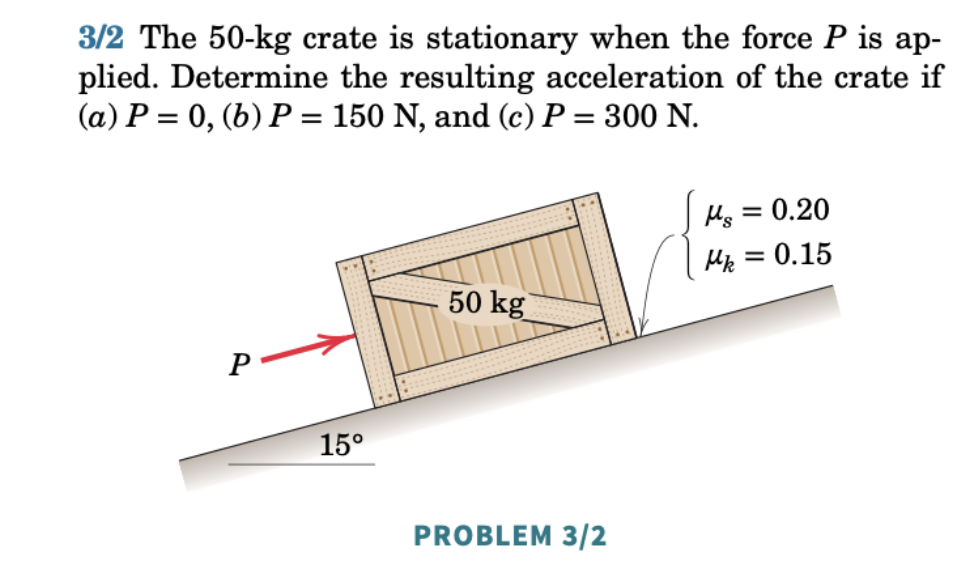
\includegraphics[width=0.5\linewidth,height=\textheight,keepaspectratio]{particle_dynamics/../figures/friction_force/03-002.png}

}

\caption{MKB 03-002.}

\end{figure}%

\textbf{2.} {[}MKB 03-030{]} Apply the 4 steps twice: first for the
combined system, then for mass \(m_2\) alone. \emph{(ans.
\(0.0577(m_1+m_2)g \le P \le 0.745(m_1+m_2)g\))}

\begin{figure}[H]

{\centering 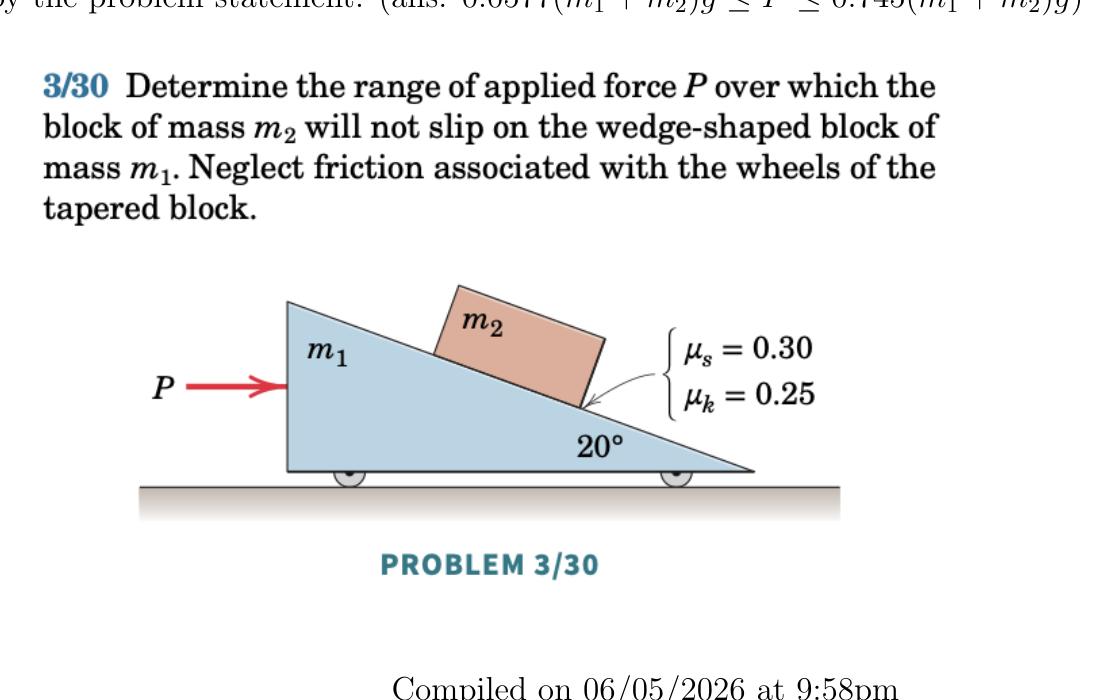
\includegraphics[width=0.5\linewidth,height=\textheight,keepaspectratio]{particle_dynamics/../figures/friction_force/03-030.png}

}

\caption{MKB 03-030.}

\end{figure}%

\textbf{3.} {[}MKB 03-047{]} Compare the Serret--Frenet basis here with
Problem 03-043 from Set 07. \emph{(ans. \(N=156.2\) lb, \(a=27.7\)
ft/sec\(^2\))}

\begin{figure}[H]

{\centering 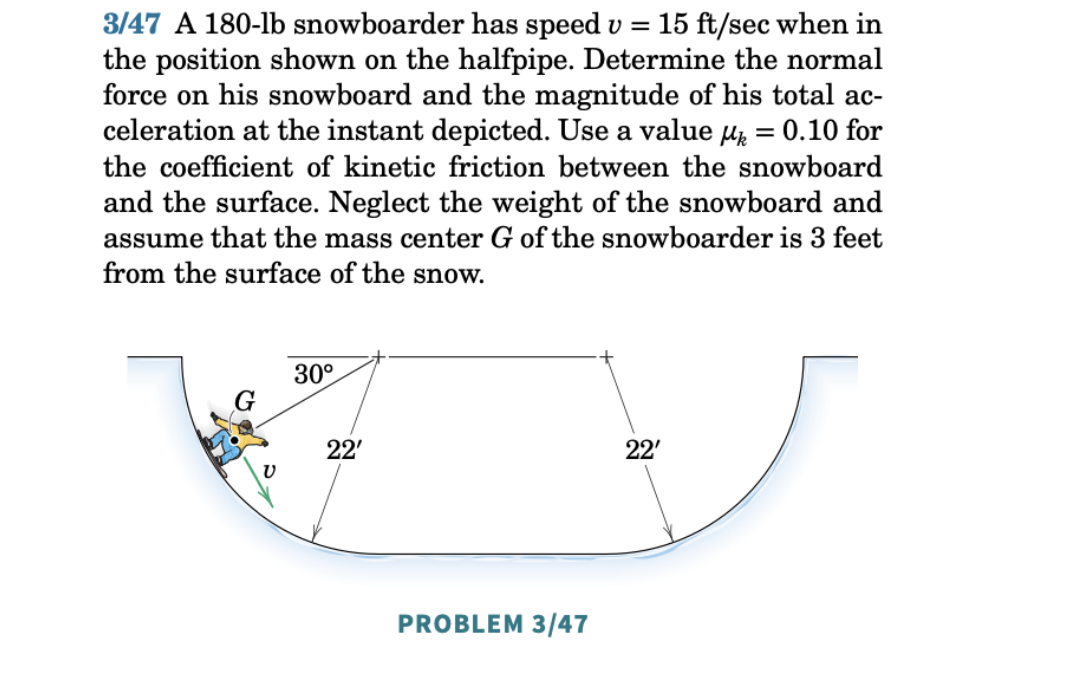
\includegraphics[width=0.5\linewidth,height=\textheight,keepaspectratio]{particle_dynamics/../figures/friction_force/03-047.png}

}

\caption{MKB 03-047.}

\end{figure}%

\textbf{4.} {[}03-049{]} Set up a cylindrical polar coordinate system
with origin at the base of the cylinder axis; apply the 4 steps to the
small object \(A\). \emph{(ans. \(\omega=\sqrt{\mu_s g/r}\))}

\begin{figure}[H]

{\centering 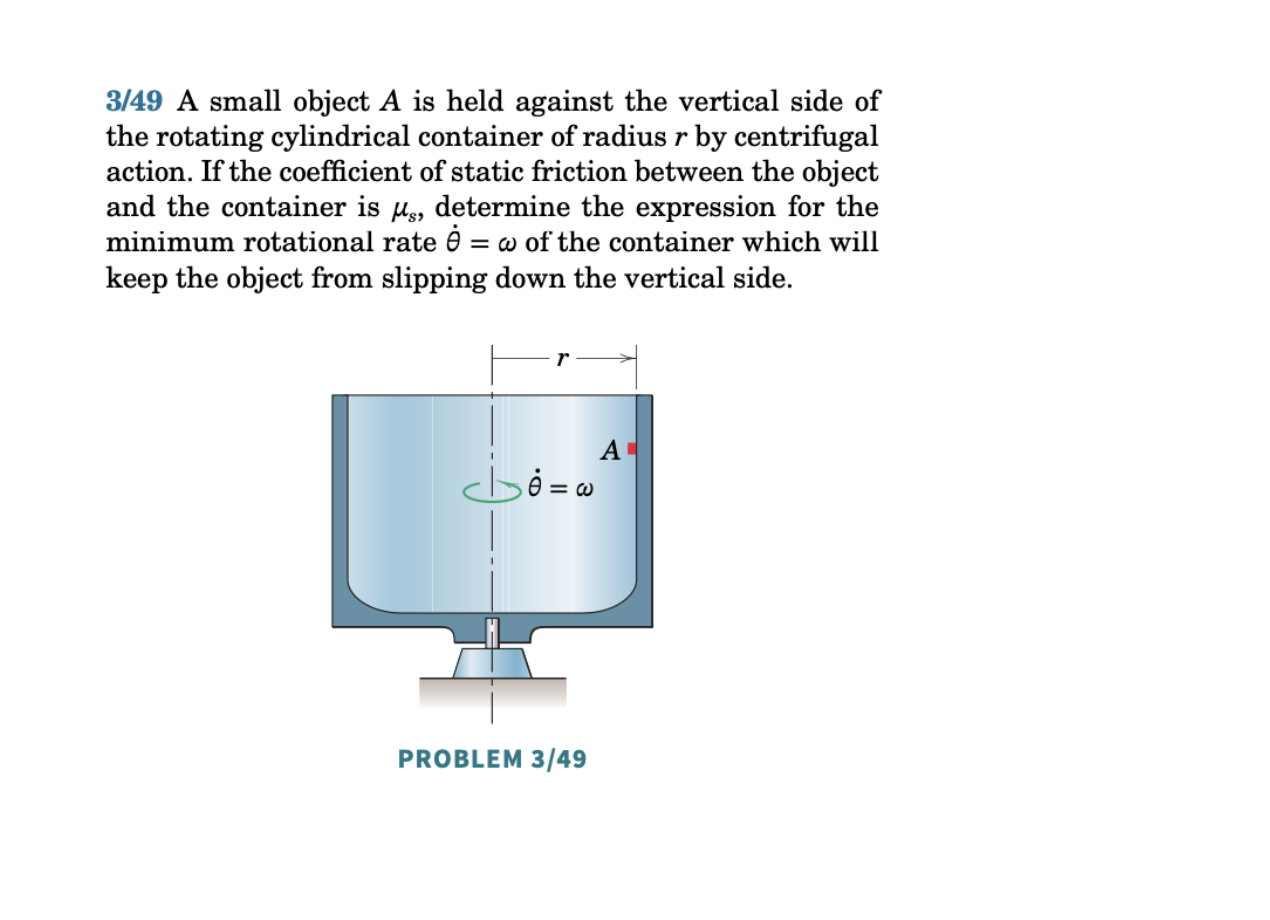
\includegraphics[width=0.5\linewidth,height=\textheight,keepaspectratio]{particle_dynamics/../figures/friction_force/03-049.png}

}

\caption{MKB 03-049.}

\end{figure}%

\textbf{5.} {[}03-050{]} This determines the maximum lateral
acceleration before slipping. \emph{(ans. \(a_n=0.818g\), \(F=2460\)
lb)}

\begin{figure}[H]

{\centering 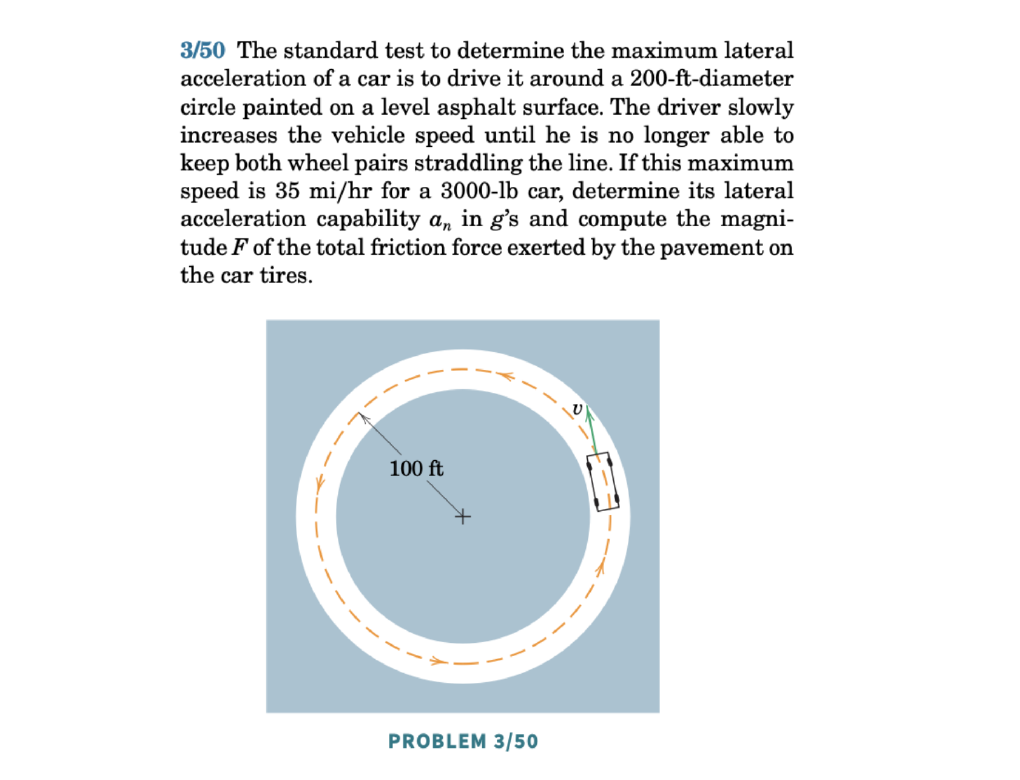
\includegraphics[width=0.5\linewidth,height=\textheight,keepaspectratio]{particle_dynamics/../figures/friction_force/03-050.png}

}

\caption{MKB 03-050.}

\end{figure}%

\textbf{6.} {[}03-071{]} Polar coordinate system with origin at the
centre of the disk. \emph{(ans.
\(N=\frac{\mu_s g}{4\pi^2}\left(\frac{1}{r\alpha}-1\right)\))}

\begin{figure}[H]

{\centering 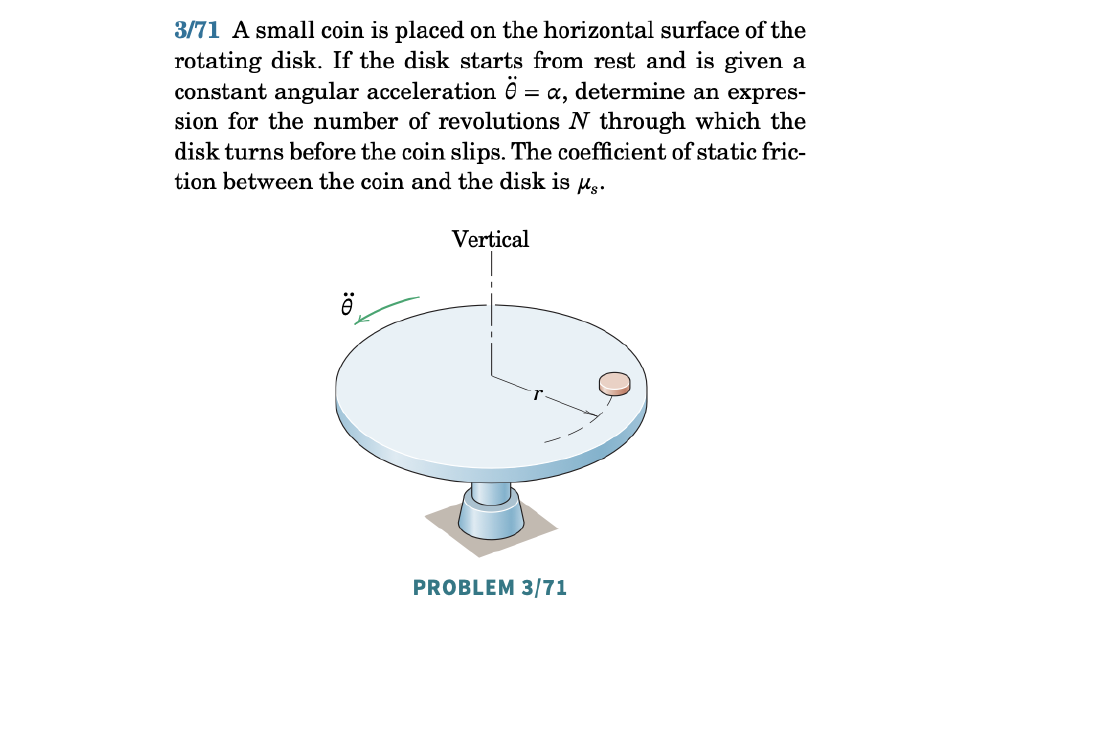
\includegraphics[width=0.5\linewidth,height=\textheight,keepaspectratio]{particle_dynamics/../figures/friction_force/03-071.png}

}

\caption{MKB 03-071.}

\end{figure}%

\url{https://youtu.be/RDFfE0tFTnk}

\chapter{Gravitational Force Model}\label{gravitational-force-model}

\begin{center}
\pandocbounded{
\includegraphics[keepaspectratio]{particle_dynamics/gravitational_force_model_files/figure-pdf/unnamed-chunk-1-1.pdf}}
\end{center}

Call \({\bf r}_2 - {\bf r}_1 = {\bf r}_{2/1}\). According to Newton's
law of gravitation, the force on \(m_1\) due to \(m_2\) is:
\begin{align}
    {\bf F}_1 = G \frac{m_1 m_2}{\lnorm{\bf r}_{2/1}\rnorm^2}\frac{{\bf r}_{2/1}}{\lnorm{\bf r}_{2/1}\rnorm} = G\frac{m_1 m_2}{\lnorm{\bf r}_{2/1}\rnorm^3}{\bf r}_{2/1}.
\end{align} where \(G = 6.67408\times10^{-11}\) m\(^3\) kg\(^{-1}\)
s\(^{-2}\) is the gravitational constant.

\section{\texorpdfstring{Example: Attraction Between Earth and an Object
of Mass
\(m\)}{Example: Attraction Between Earth and an Object of Mass m}}\label{example-attraction-between-earth-and-an-object-of-mass-m}

\begin{center}
\pandocbounded{
\includegraphics[keepaspectratio]{particle_dynamics/gravitational_force_model_files/figure-pdf/unnamed-chunk-2-1.pdf}}
\end{center}

\begin{align}
    {\bf F} = G\frac{M_e m}{\lp R_e+h\rp^2}\lp-{\bf E}_z\rp.
\end{align}

Since \(h \ll R_e\), we have \(\lp R_e+h\rp^2 \approx R_e^2\), giving:
\begin{align}
    {\bf F} = G\frac{M_e}{R_e^2}m\lp-{\bf E}_z\rp = mg\lp-{\bf E}_z\rp,
\end{align} where \(g = G M_e / R_e^2 = 9.81\) m/s\(^2 = 32.2\)
ft/s\(^2\).

Earth's parameters:

\begin{itemize}
\tightlist
\item
  \(M_e = 5.972 \times 10^{24}\) kg
\item
  \(R_e = 6.371 \times 10^6\) m
\end{itemize}

\url{https://youtu.be/nHnDuCWtacY}

\chapter{Power, Work, and Energy}\label{power-work-and-energy}

\section{Power and Work}\label{power-and-work}

The \textbf{mechanical power} of a force \({\bf F}\) acting on a
particle with absolute velocity \({\bf v}\) is: \begin{align}
    \mathcal{P} = {\bf F}\cdot{\bf v}.
\end{align}

The \textbf{work} done by \({\bf F}\) over the interval \([t_1,t_2]\)
is: \begin{align}
    W_{{\bf F},12} = \int_{t_1}^{t_2} {\bf F}\cdot{\bf v}\,dt = \int_{t_1}^{t_2}{\bf F}\cdot d{\bf r},
\end{align} since \(d{\bf r} = {\bf v}\,dt\). So power is the derivative
of work: \(\mathcal{P} = \dot{W}\).

In SI units: work is in Newton meters (Joules) and power in Watts.

Notes:

\begin{itemize}
\tightlist
\item
  There are many representations of this integral depending on the
  coordinate system:

  \begin{itemize}
  \tightlist
  \item
    Cartesian: \(d{\bf r} = dx{\bf E}_x+dy{\bf E}_y+dz{\bf E}_z\)
  \item
    Polar: \(d{\bf r} = dr{\bf e}_r+r\,d\theta{\bf e}_\theta\)
  \item
    Serret-Frenet: \(d{\bf r} = ds\,{\bf e}_t\)
  \end{itemize}
\item
  This integral is \textbf{path dependent} --- we need to know the
  particle's path to compute it.
\end{itemize}

\begin{tcolorbox}[enhanced jigsaw, arc=.35mm, bottomrule=.15mm, bottomtitle=1mm, breakable, colback=white, colbacktitle=quarto-callout-tip-color!10!white, colframe=quarto-callout-tip-color-frame, coltitle=black, left=2mm, leftrule=.75mm, opacityback=0, opacitybacktitle=0.6, rightrule=.15mm, title=\textcolor{quarto-callout-tip-color}{\faLightbulb}\hspace{0.5em}{Think!}, titlerule=0mm, toprule=.15mm, toptitle=1mm]

\textbf{Question:} In what case would the work of a force be zero?

\begin{quote}
\textbf{Answer}

The work is zero if the force is perpendicular to the
displacement/velocity, or if the force is applied at a fixed point.
\end{quote}

\end{tcolorbox}

\begin{tcolorbox}[enhanced jigsaw, arc=.35mm, bottomrule=.15mm, bottomtitle=1mm, breakable, colback=white, colbacktitle=quarto-callout-tip-color!10!white, colframe=quarto-callout-tip-color-frame, coltitle=black, left=2mm, leftrule=.75mm, opacityback=0, opacitybacktitle=0.6, rightrule=.15mm, title=\textcolor{quarto-callout-tip-color}{\faLightbulb}\hspace{0.5em}{Think!}, titlerule=0mm, toprule=.15mm, toptitle=1mm]

\textbf{Question:} When is the work of a force positive? When is it
negative?

\begin{quote}
\textbf{Answer}

\ldots{}
\end{quote}

\end{tcolorbox}

\subsection{Example: Particle on a
Rail}\label{example-particle-on-a-rail}

Consider two points \(A\) and \(B\) in the vertical plane connected by a
smooth rail. A particle slides along the rail from \(B\) to \(A\).

\begin{center}
\pandocbounded{
\includegraphics[keepaspectratio]{particle_dynamics/power_work_energy_files/figure-pdf/unnamed-chunk-1-1.pdf}}
\end{center}

\begin{tcolorbox}[enhanced jigsaw, arc=.35mm, bottomrule=.15mm, bottomtitle=1mm, breakable, colback=white, colbacktitle=quarto-callout-tip-color!10!white, colframe=quarto-callout-tip-color-frame, coltitle=black, left=2mm, leftrule=.75mm, opacityback=0, opacitybacktitle=0.6, rightrule=.15mm, title=\textcolor{quarto-callout-tip-color}{\faLightbulb}\hspace{0.5em}{Think!}, titlerule=0mm, toprule=.15mm, toptitle=1mm]

\textbf{Question:} What is the work done by forces on an object
traveling from \(A\) to \(B\) on (a) a straight rail or (b) a curved
path?

\begin{quote}
\textbf{Answer}

In both cases \({\bf F} = {\bf W}+{\bf N}\). Since
\({\bf N}\perp d{\bf r}\), the normal force does no work. The work of
weight is: \begin{align*}
    W_{{\bf W},1-2} = \int_{{\bf r}_1}^{{\bf r}_2} mg{\bf E}_y\cdot d{\bf r} = mg {\bf E}_y\cdot \int_{{\bf r}_1}^{{\bf r}_2} d{\bf r} = mg{\bf E}_y\cdot\Delta {\bf r}_{1-2}.
\end{align*} \(\Delta{\bf r}_{1-2}\) is the same for both rails, so
weight does the same work regardless of path.
\end{quote}

\end{tcolorbox}

\begin{tcolorbox}[enhanced jigsaw, arc=.35mm, bottomrule=.15mm, bottomtitle=1mm, breakable, colback=white, colbacktitle=quarto-callout-tip-color!10!white, colframe=quarto-callout-tip-color-frame, coltitle=black, left=2mm, leftrule=.75mm, opacityback=0, opacitybacktitle=0.6, rightrule=.15mm, title=\textcolor{quarto-callout-tip-color}{\faLightbulb}\hspace{0.5em}{Think!}, titlerule=0mm, toprule=.15mm, toptitle=1mm]

\textbf{Question:} What changes if the rail is rough?

\begin{quote}
\textbf{Answer}

With friction: \begin{align*}
    W_{1-2} = W_{{\bf W},1-2}+\int_{s_1}^{s_2}\mu_k||{\bf N}||(-{\bf e}_t)\cdot ds\,{\bf e}_t = W_{{\bf W},1-2}-\mu_k\int_{s_1}^{s_2}||{\bf N}||ds.
\end{align*} Friction work is path dependent and dissipative
(\(W_{{\bf F}_f,1-2}<0\)). On the other hand, the work of the weight is
positive.
\end{quote}

\end{tcolorbox}

\begin{tcolorbox}[enhanced jigsaw, arc=.35mm, bottomrule=.15mm, bottomtitle=1mm, breakable, colback=white, colbacktitle=quarto-callout-tip-color!10!white, colframe=quarto-callout-tip-color-frame, coltitle=black, left=2mm, leftrule=.75mm, opacityback=0, opacitybacktitle=0.6, rightrule=.15mm, title=\textcolor{quarto-callout-tip-color}{\faLightbulb}\hspace{0.5em}{Think!}, titlerule=0mm, toprule=.15mm, toptitle=1mm]

\textbf{Question:} Can you think of a situation where the normal force
is not workless?

\begin{quote}
\textbf{Answer}

A particle in an elevator is a common example. In this case, the normal
force is not perpendicular to the motion, and it does work.
\end{quote}

\end{tcolorbox}

\section{Kinetic Energy}\label{kinetic-energy}

The \textbf{kinetic energy} of a particle: \begin{align}
    T = \frac{m}{2}{\bf v}\cdot{\bf v}.
\end{align}

In different bases: \begin{align*}
    T = \frac{1}{2}m(v_x^2+v_y^2+v_z^2) = \frac{1}{2}m(\dot{r}^2+r^2\dot{\theta}^2+\dot{z}^2) = \frac{1}{2}mv^2.
\end{align*}

\section{Energy}\label{energy}

Energy is defined as the ability to perform work.

\section{The Work-Energy Theorem}\label{the-work-energy-theorem}

The rate of change of kinetic energy equals the mechanical power of the
resultant force \({\bf F}\) acting on the particle: \begin{align}
    \frac{dT}{dt} = {\bf F}\cdot{\bf v} = \mathcal{P}.
\end{align}

Proof: \begin{align*}
    \frac{d}{dt}T = \frac{d}{dt}\lp\frac{1}{2}m{\bf v}\cdot{\bf v}\rp = m{\bf a}\cdot{\bf v} = {\bf F}\cdot{\bf v}.
\end{align*}

Integral form (with respect to time): \begin{align}
    T_2 - T_1 = W_{{\bf F},12} = \int_{{\bf r}_1}^{{\bf r}_2}{\bf F}\cdot d{\bf r}.
\end{align}

\url{https://www.youtube.com/watch?v=bjpTKehJV7s}

\section{\texorpdfstring{Implications of
\(\dot{T} = {\bf F}\cdot{\bf v}\) through
examples}{Implications of \textbackslash dot\{T\} = \{\textbackslash bf F\}\textbackslash cdot\{\textbackslash bf v\} through examples}}\label{implications-of-dott-bf-fcdotbf-v-through-examples}

\begin{itemize}
\item
  Consider a free falling particle. The weight is the only force acting
  on it. If the particle is going up (opposite to the weight),
  \(\dot{T}<0\). If the particle is going down (same direction of the
  weight), \(\dot{T}>0\).
\item
  Consider a person standing on a train while the train is accelerating:
  \begin{align}
  & {\bf F} = {\bf W}+{\bf F}_f+{\bf N}\\
  & {\bf F}\cdot{\bf v} = {\bf F}_f\cdot{\bf v} \geq 0 \implies \dot{T}>0.
  \end{align} The kinetic energy of the person is increasing.
\item
  Consider a box sliding on a rough surface: \begin{align}
  & {\bf F} = {\bf F}_f+{\bf W}+{\bf N}\\
  & {\bf F}\cdot{\bf v} = {\bf F}_f\cdot{\bf v} < 0 \implies \dot{T}<0.
  \end{align} The kinetic energy of the box is decreasing until it
  stops.
\item
  Consider a particle on a smooth rail in the horizontal plane:
  \begin{align}
  & {\bf F} = {\bf W}+{\bf N}\\
  & {\bf F}\cdot{\bf v} = 0\implies\dot{T}=0.
  \end{align} The kinetic energy of the particle is conserved.
\end{itemize}

The same analysis/conclusions can be achieved using the work-energy
theorem.

\section{Another way to derive the Work-Energy
theorem}\label{another-way-to-derive-the-work-energy-theorem}

Starting with the balance of linear momentum we can derive the
work-energy theorem: \begin{align}
{\bf F} &= m{\bf a}\\
{\bf F}\cdot d{\bf r} &= m{\bf a}\cdot d{\bf r}\\
\int_{r_1}^{r_2} {\bf F}\cdot d{\bf r} &= \int_{r_1}^{r_2} m{\bf a}\cdot d{\bf r}\\
W_{1-2} &= \int_{t_1}^{t_2} m{\bf a}\cdot {\bf v}\, dt = \int_{t_1}^{t_2}\dot{T}\, dt = T_2-T_1,
\end{align} where the work of a force is
\[W_{1-2} = \int_{r_1}^{r_2} {\bf F}\cdot d{\bf r}.\]

\section{Conservative Forces}\label{conservative-forces}

Forces whose work depends only on the endpoints of a path are
\textbf{conservative}. From the previous examples, weight (constant
force) is conservative; friction is not.

A force \({\bf F}_c\) is conservative if there exists a scalar
\textbf{potential energy} function \(U = U({\bf r})\) such that:
\begin{align}
    {\bf F}_c = -\frac{\partial U}{\partial {\bf r}} = -\text{grad}_{\bf r}U.
\end{align}

Then: \begin{align}
    W_{1-2} = \int_{{\bf r}(t_1)}^{{\bf r}(t_2)}{\bf F}_c\cdot d{\bf r} = -\int_{{\bf r}(t_1)}^{{\bf r}(t_2)}\frac{\partial U}{\partial {\bf r}}\cdot d{\bf r} = -U_2+U_1 = -\Delta_{1-2}U.
\end{align}

If potential energy decreases (\(U_2 \leq U_1\)), the work is positive
and kinetic energy increases.

\begin{tcolorbox}[enhanced jigsaw, arc=.35mm, bottomrule=.15mm, bottomtitle=1mm, breakable, colback=white, colbacktitle=quarto-callout-tip-color!10!white, colframe=quarto-callout-tip-color-frame, coltitle=black, left=2mm, leftrule=.75mm, opacityback=0, opacitybacktitle=0.6, rightrule=.15mm, title=\textcolor{quarto-callout-tip-color}{\faLightbulb}\hspace{0.5em}{Think!}, titlerule=0mm, toprule=.15mm, toptitle=1mm]

\textbf{Question:} Consider a particle thrown from the top of a
building. Describe the changes in kinetic and potential energy of the
particle during its motion.

\begin{quote}
\textbf{Answer}

When the particle is still high, its potential energy is high and its
kinetic energy is low. When the particle has traveled downward, its
potential energy is low and its kinetic energy is high.
\end{quote}

\end{tcolorbox}

\subsection{Constant Forces}\label{constant-forces}

Constant force \({\bf C}\) is conservative with potential
\(U = -{\bf C}\cdot{\bf r}\).

Proof: Propose
\(U = -{\bf C}\cdot{\bf r} = U({\bf r}) = -C_x x-C_y y-C_z z\).
\begin{align}
    -\text{grad}_r{U} = C_x{\bf E}_x+C_y{\bf E}_y+C_z{\bf E}_z = {\bf C}.
\end{align} We found a \(U\) from which \({\bf C}\) is derivable.

The weight near Earth's surface: \(U_{\bf W} = mgy\).

\subsection{Spring Force}\label{spring-force-1}

The spring force is conservative with potential: \begin{align*}
    U_s = \frac{1}{2}K\varepsilon^2.
\end{align*} \(U_s > 0\) in both compression and tension --- it
represents the spring's capacity to do work.

Proof: \begin{align*}
    & -\frac{\partial U_s}{\partial {\bf r}} = K\varepsilon\frac{{\bf r}_A-{\bf r}}{||{\bf r}_A-{\bf r}||} = {\bf F}_s.
\end{align*}

\subsection{Gravitational Force}\label{gravitational-force-1}

The gravitational force
\({\bf F}_G = G\frac{M_e m}{\lp R_e+h\rp^2}\lp-{\bf e}_r\rp\) is
conservative with: \begin{align*}
    U = -\frac{GM_e m}{r}.
\end{align*}

Drag, friction, tension in inextensible cables, and normal forces are
nonconservative.

\section{Energy and Its Conservation}\label{energy-and-its-conservation}

If only conservative forces act, define total mechanical energy
\(E = T + U\). Then: \begin{align*}
    & \dot{T} = {\bf F}_c\cdot{\bf V} = -\frac{\partial U}{\partial {\bf r}}\cdot\dot{\bf r} = -\dot{U}\\
    & \dot{T} = -\dot{U} \implies \dot{E} = \dot{T}+\dot{U} = 0.
\end{align*} \(E\) is conserved when all work-doing forces are
conservative, ie. \({\bf F}\cdot{\bf v}={\bf F}_c\cdot{\bf v}\).

If nonconservative forces also act: \begin{align}
    E_B - E_A = W_{{\bf F}_{nc},AB}.
\end{align}

\subsection{Example: Smooth vs.~Rough
Rail}\label{example-smooth-vs.-rough-rail}

\emph{Smooth rail:}
\({\bf F}\cdot{\bf v} = {\bf W}\cdot{\bf v}+{\bf N}\cdot{\bf v} = {\bf W}\cdot{\bf v} = -\dot{U}\),
so \(\dot{E} = 0\).

\emph{Rough rail:} \(\dot{E} = {\bf F}_f\cdot{\bf v} < 0\), so energy
bleeds off over time. Integrating: \begin{align*}
    E(t_2) = E(t_1) + W_{{\bf F}_f,1-2} < E(t_1).
\end{align*}

\section{Summary}\label{summary-8}

\textbf{Power} of force \(\mathbf{F}\) on particle with velocity
\(\mathbf{v}\): \(P = \mathbf{F}\cdot\mathbf{v}\).

\textbf{Work--energy theorem}: \(T_B - T_A = W_{\mathbf{F},AB}\), where
\(T=\tfrac{1}{2}m\mathbf{v}\cdot\mathbf{v}\).

\textbf{Conservative forces} satisfy \(W_{F_c,AB}=-(U_B-U_A)\).
Including non-conservative work: \begin{align}
    (T_B+U_B)-(T_A+U_A) = W_{\mathbf{F}_{nc},AB}.
\end{align} If all work-doing forces are conservative, \textbf{energy is
conserved}: \(E=T+U=\text{const}\).

\section{Exercises}\label{exercises-10}

\emph{The following problems are from Set 11 -- Power, Work and Energy.}

\textbf{1.} {[}MKB 03-128{]} Only the gravitational force acts on the
spacecraft, so energy is conserved. Use conservation of energy.
\emph{(ans. \(v_B = 26\,300\) km/h)}

\begin{figure}[H]

{\centering 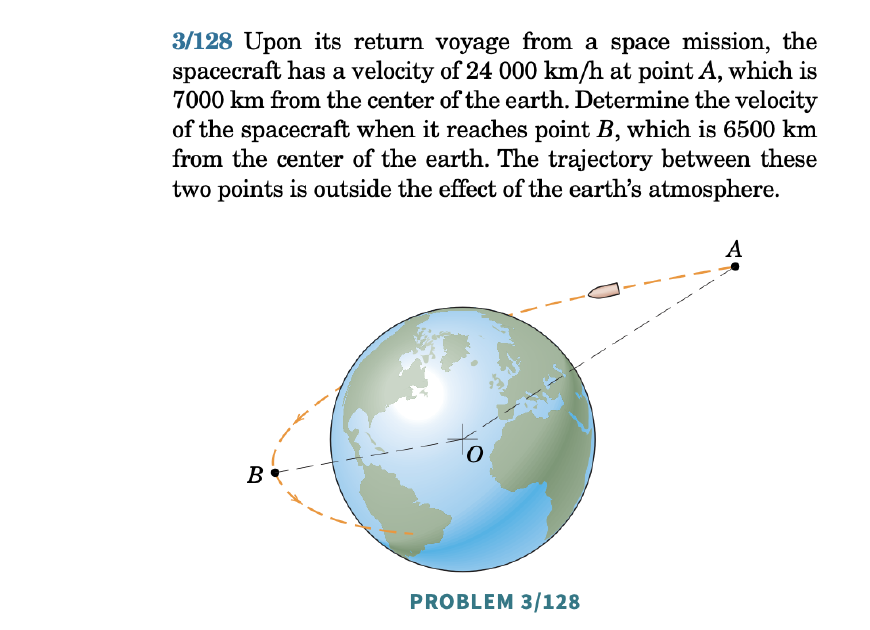
\includegraphics[width=0.5\linewidth,height=\textheight,keepaspectratio]{particle_dynamics/../figures/power_work_energy/03-128.png}

}

\caption{MKB 03-128.}

\end{figure}%

\textbf{2.} {[}MKB 03-080{]} \emph{(ans. (a) no motion; (b)
\(v_B = 5.62\) m/s)}

\begin{figure}[H]

{\centering 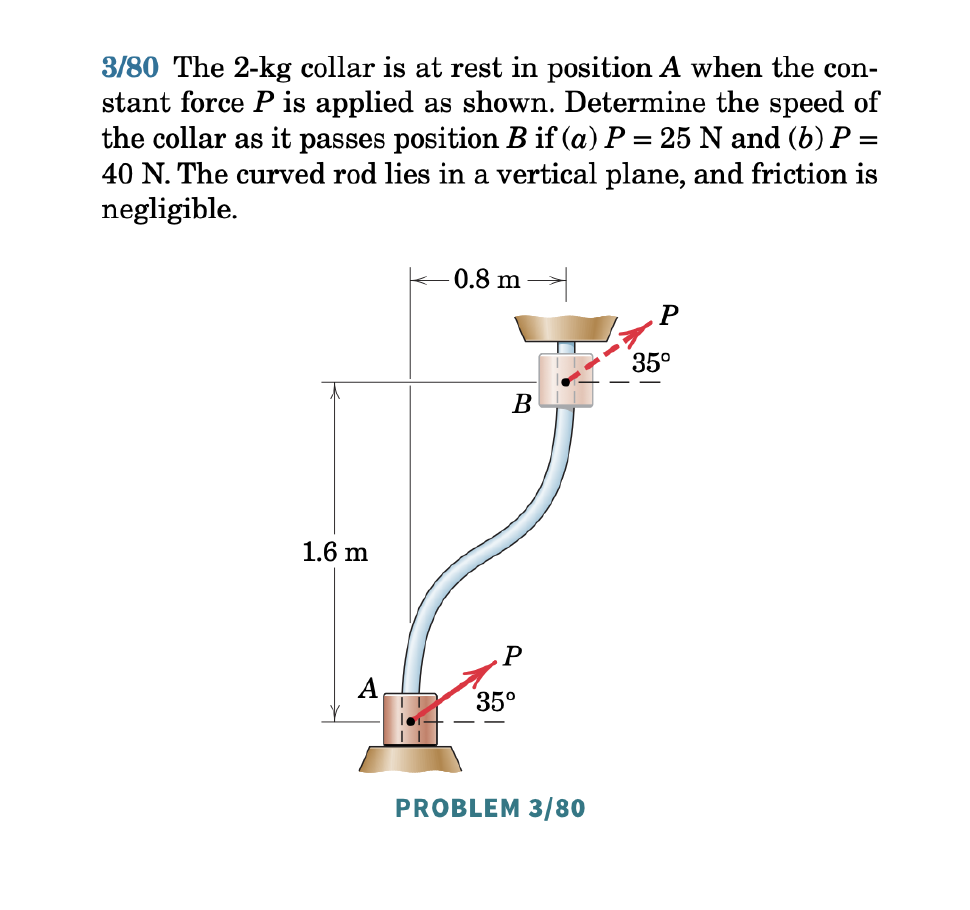
\includegraphics[width=0.5\linewidth,height=\textheight,keepaspectratio]{particle_dynamics/../figures/power_work_energy/03-080.png}

}

\caption{MKB 03-080.}

\end{figure}%

\textbf{3.} {[}MKB 03-084{]} \emph{(ans. (a) \(v=2.56\) m/s; (b)
\(x=98.9\) mm)}

\begin{figure}[H]

{\centering 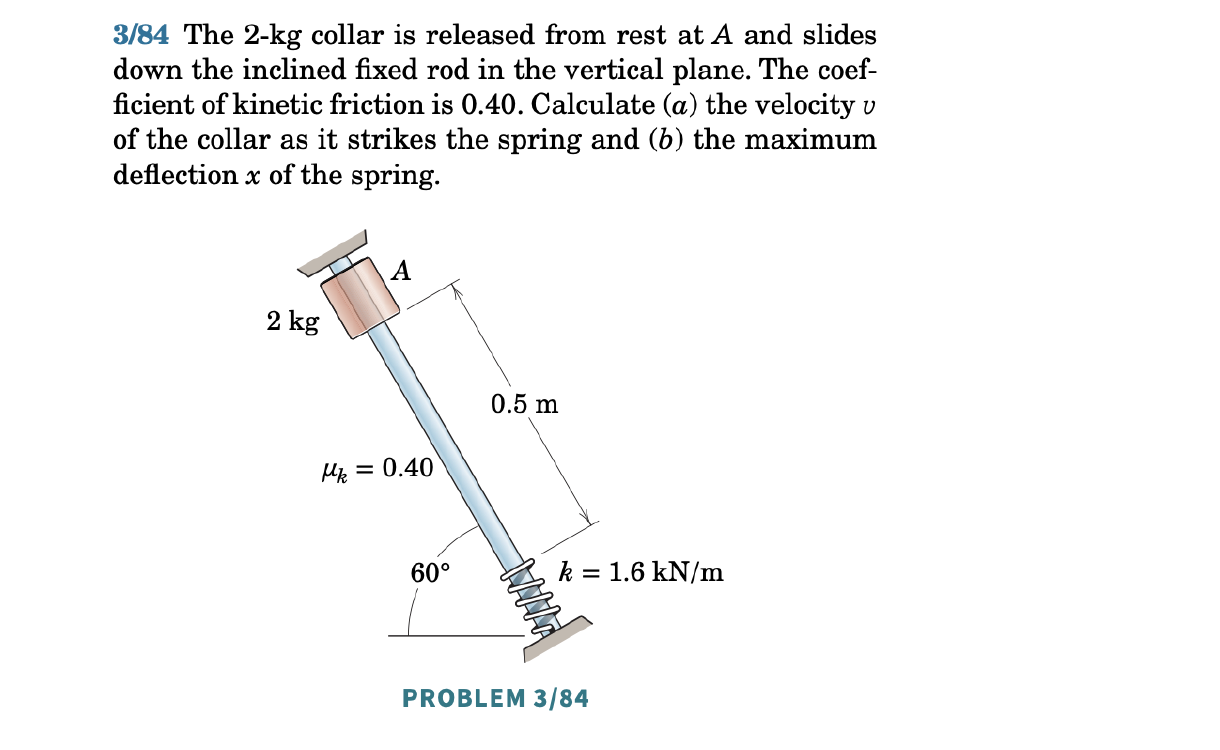
\includegraphics[width=0.5\linewidth,height=\textheight,keepaspectratio]{particle_dynamics/../figures/power_work_energy/03-084.png}

}

\caption{MKB 03-084.}

\end{figure}%

\textbf{4.} {[}MKB 03-094{]} \emph{(ans. (a) \(N_B=48\) N right; (b)
\(N_B'=29.4\) N right; (c) \(N_C=17.63\) N down; (d) \(N_D=29.4\) N
left)}

\begin{figure}[H]

{\centering 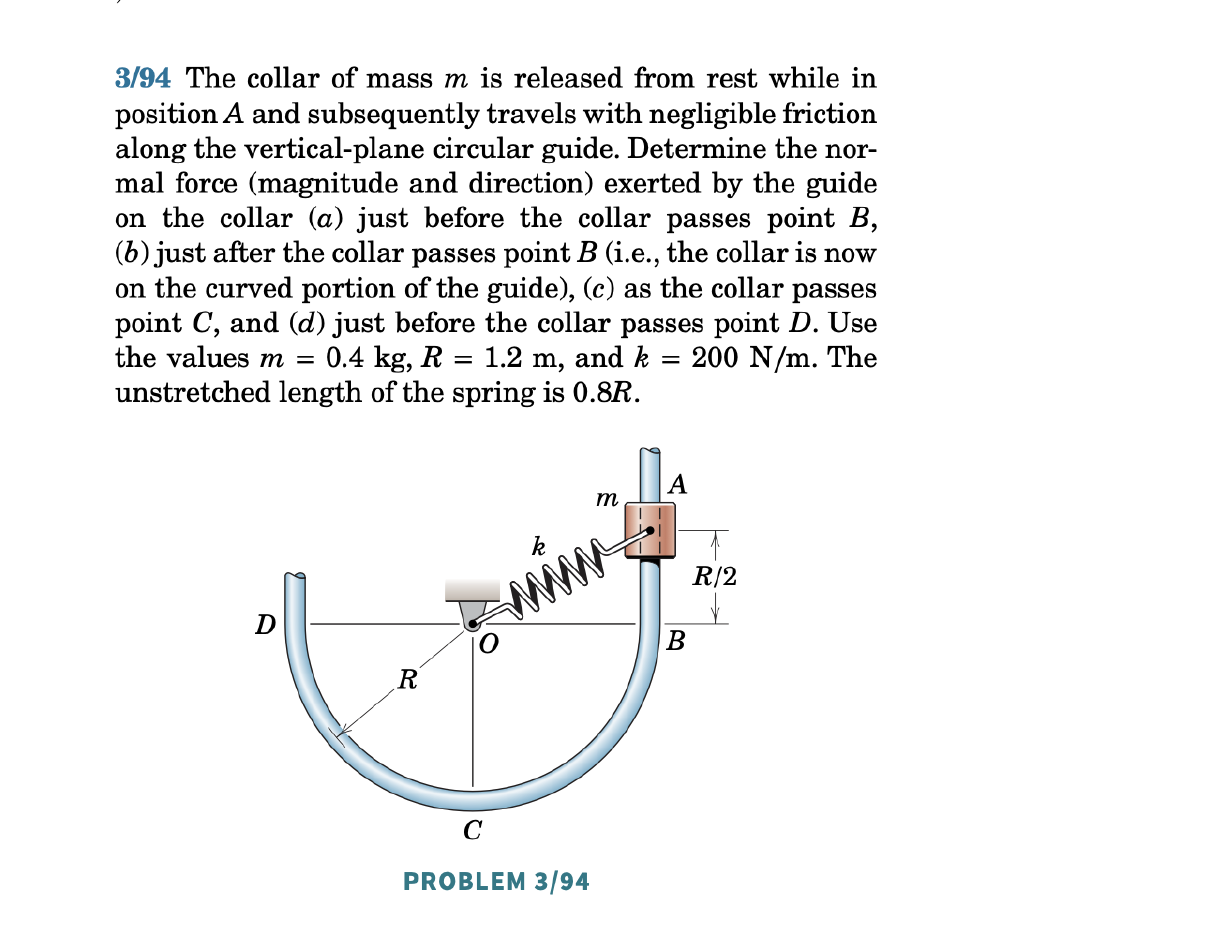
\includegraphics[width=0.5\linewidth,height=\textheight,keepaspectratio]{particle_dynamics/../figures/power_work_energy/03-094.png}

}

\caption{MKB 03-094.}

\end{figure}%

\textbf{5.} {[}MKB 03-101{]} \emph{(ans. (a) \(N_B=4mg\); (b)
\(N_C=7mg\); (c) \(s=\frac{4R}{\sqrt{3}(1+\mu_k)}\))}

\begin{figure}[H]

{\centering 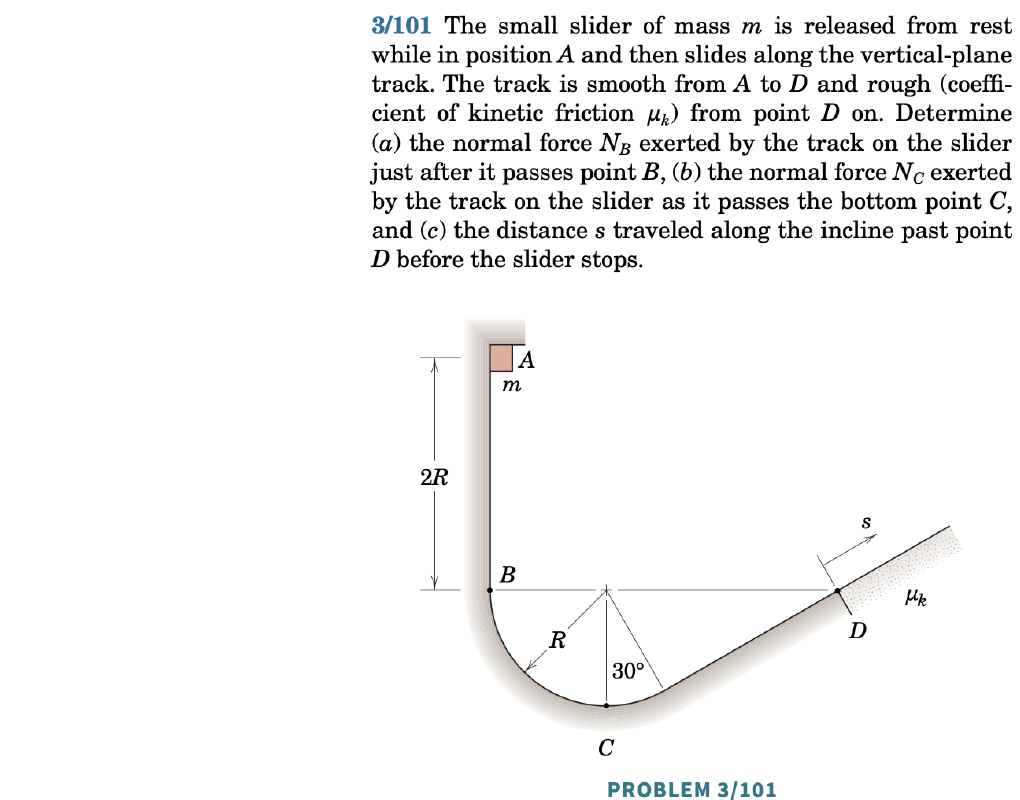
\includegraphics[width=0.5\linewidth,height=\textheight,keepaspectratio]{particle_dynamics/../figures/power_work_energy/03-101.png}

}

\caption{MKB 03-101.}

\end{figure}%

\textbf{6.} {[}MKB 03-263{]} \emph{(ans. \(R=46.7\) N)}

\begin{figure}[H]

{\centering 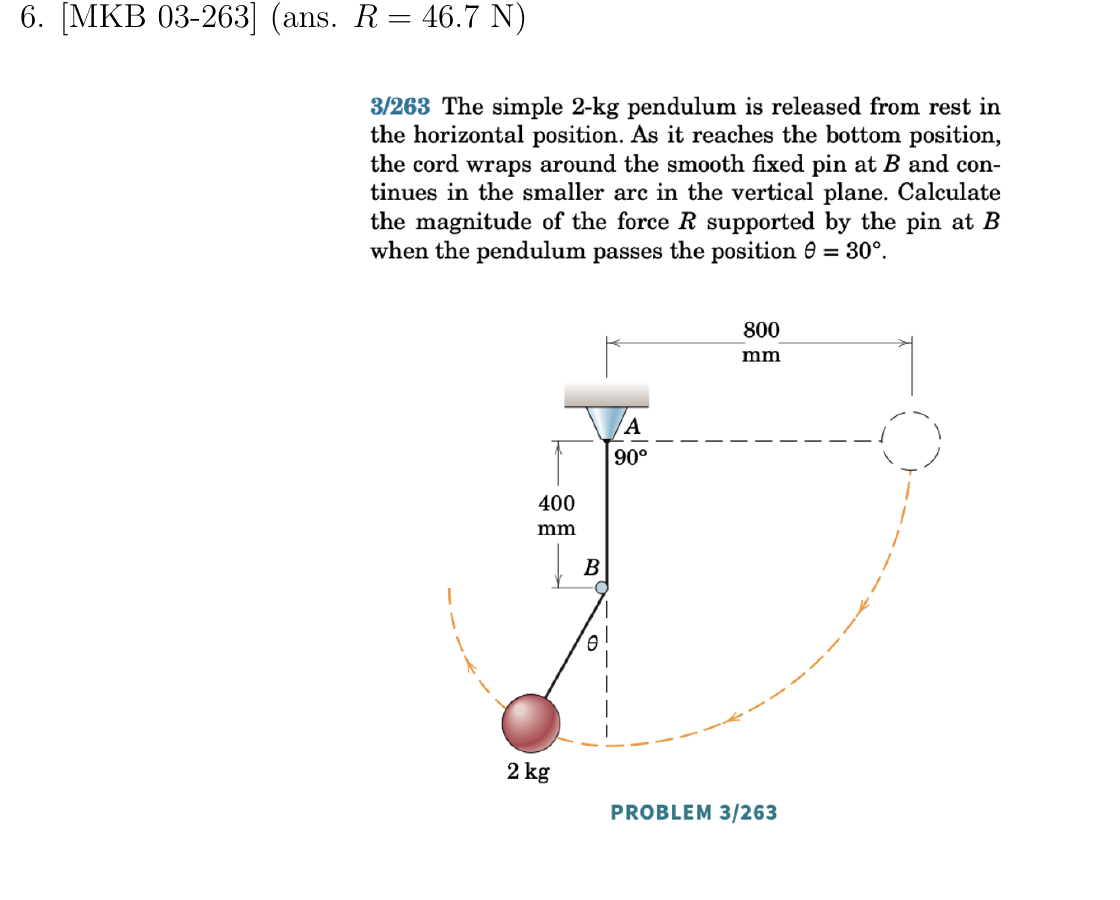
\includegraphics[width=0.5\linewidth,height=\textheight,keepaspectratio]{particle_dynamics/../figures/power_work_energy/03-263.png}

}

\caption{MKB 03-263.}

\end{figure}%

\textbf{7.} {[}OOR Exercise 5-1{]}

\begin{figure}[H]

{\centering 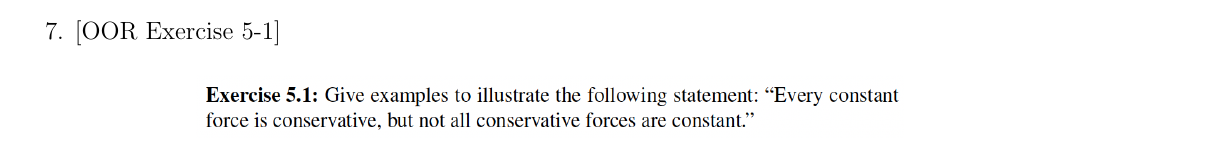
\includegraphics[width=0.7\linewidth,height=\textheight,keepaspectratio]{particle_dynamics/../figures/power_work_energy/oor_5_1.png}

}

\caption{O'Reilly Primer, Exercise 5.1.}

\end{figure}%

\textbf{8.} {[}OOR Exercise 5-4{]}

\begin{figure}[H]

{\centering 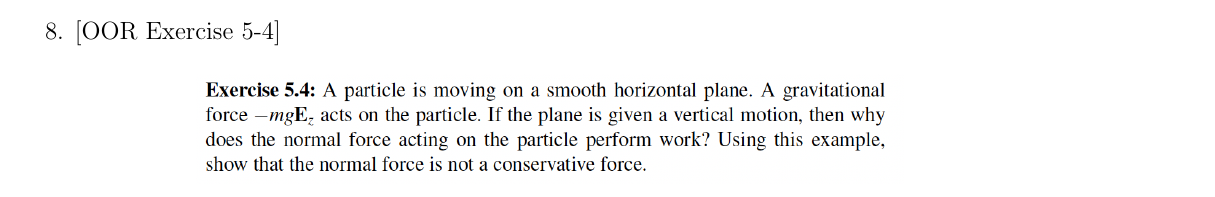
\includegraphics[width=0.7\linewidth,height=\textheight,keepaspectratio]{particle_dynamics/../figures/power_work_energy/oor_5_4.png}

}

\caption{O'Reilly Primer, Exercise 5.4.}

\end{figure}%

\textbf{9.} {[}OOR Exercises 5-6 \& 5-7{]}

\begin{figure}[H]

{\centering 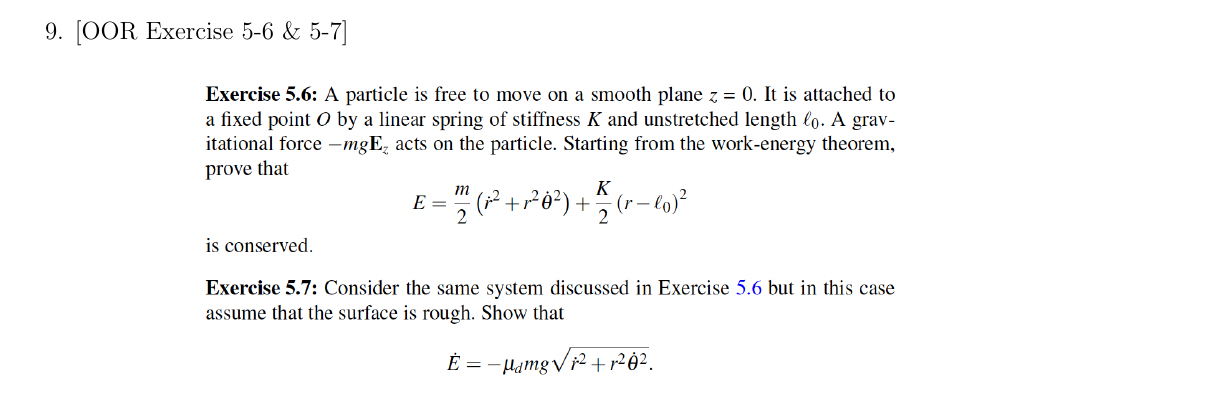
\includegraphics[width=0.7\linewidth,height=\textheight,keepaspectratio]{particle_dynamics/../figures/power_work_energy/oor_5_6_7.png}

}

\caption{O'Reilly Primer, Exercises 5.6 and 5.7.}

\end{figure}%

\textbf{10.} {[}OOR Exercises 5-8 \& 5-9{]}

\begin{figure}[H]

{\centering 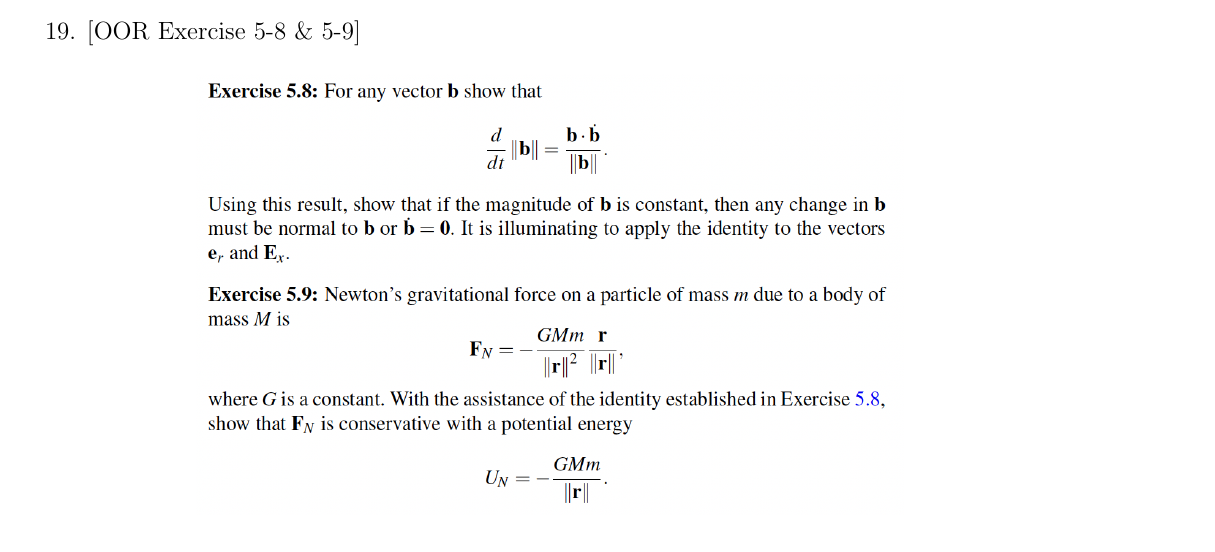
\includegraphics[width=0.7\linewidth,height=\textheight,keepaspectratio]{particle_dynamics/../figures/power_work_energy/oor_5_8_9.png}

}

\caption{O'Reilly Primer, Exercises 5.8 and 5.9.}

\end{figure}%

\chapter{Momenta and Impulses of
Particles}\label{momenta-and-impulses-of-particles}

\section{Linear Momentum and Its
Conservation}\label{linear-momentum-and-its-conservation}

Recall the linear momentum \({\bf G} = m{\bf v}\).

\subsection{Linear Impulse and Linear
Momentum}\label{linear-impulse-and-linear-momentum}

The integral form of the balance of linear momentum: \begin{align}
    {\bf G}(t_1)-{\bf G}(t_0) = \int_{t_0}^{t_1}{\bf F}\,dt.
\end{align}

The time integral of a force is its \textbf{linear impulse}. This form
is more general than \({\bf F}=m{\bf a}\) because it does not require
\({\bf v}\) to be differentiable.

\url{https://youtu.be/-AHQOYy3VBk}

\subsection{Conservation of Linear
Momentum}\label{conservation-of-linear-momentum}

\begin{tcolorbox}[enhanced jigsaw, arc=.35mm, bottomrule=.15mm, bottomtitle=1mm, breakable, colback=white, colbacktitle=quarto-callout-tip-color!10!white, colframe=quarto-callout-tip-color-frame, coltitle=black, left=2mm, leftrule=.75mm, opacityback=0, opacitybacktitle=0.6, rightrule=.15mm, title=\textcolor{quarto-callout-tip-color}{\faLightbulb}\hspace{0.5em}{Think!}, titlerule=0mm, toprule=.15mm, toptitle=1mm]

\textbf{Question:} Under what conditions is the linear momentum of a
system conserved?

\begin{quote}
\textbf{Answer}

\ldots{}
\end{quote}

\end{tcolorbox}

\begin{tcolorbox}[enhanced jigsaw, arc=.35mm, bottomrule=.15mm, bottomtitle=1mm, breakable, colback=white, colbacktitle=quarto-callout-tip-color!10!white, colframe=quarto-callout-tip-color-frame, coltitle=black, left=2mm, leftrule=.75mm, opacityback=0, opacitybacktitle=0.6, rightrule=.15mm, title=\textcolor{quarto-callout-tip-color}{\faLightbulb}\hspace{0.5em}{Think!}, titlerule=0mm, toprule=.15mm, toptitle=1mm]

\textbf{Question:} Under what conditions is the linear momentum of a
system conserved in a direction \({\bf c}\)?

\begin{quote}
\textbf{Answer}

Suppose that the component of \({\bf G}\) in the direction of a given
vector \({\bf c}\) is conserved: \begin{align}
    \frac{d}{dt}({\bf G}\cdot{\bf c}) = 0.
\end{align} This means that \begin{align}
    \dot{\bf G}\cdot{\bf c}+{\bf G}\cdot\dot{\bf c} = {\bf F}\cdot{\bf c}+{\bf G}\cdot\dot{\bf c} = 0.
\end{align} Thus, given a vector \({\bf c}\),
\[{\bf G}\cdot{\bf c} \text{ is conserved if, and only if, } {\bf F}\cdot{\bf c}+{\bf G}\cdot\dot{\bf c} = 0.\]
If \({\bf c}\) is a constant vector, \({\bf G}\cdot{\bf c}\) is
conserved if, and only if, \({\bf F}\cdot{\bf c} = 0\). From the BoLM,
this means that there is no force in this constant direction.
\end{quote}

\end{tcolorbox}

\url{https://youtu.be/_3a0CbiLJ18}

\subsection{Example}\label{example-1}

\begin{tcolorbox}[enhanced jigsaw, arc=.35mm, bottomrule=.15mm, bottomtitle=1mm, breakable, colback=white, colbacktitle=quarto-callout-warning-color!10!white, colframe=quarto-callout-warning-color-frame, coltitle=black, left=2mm, leftrule=.75mm, opacityback=0, opacitybacktitle=0.6, rightrule=.15mm, title=\textcolor{quarto-callout-warning-color}{\faExclamationTriangle}\hspace{0.5em}{Example}, titlerule=0mm, toprule=.15mm, toptitle=1mm]

\textbf{Question:} Is the linear momentum of a projectile conserved? In
a certain direction?

\begin{quote}
\textbf{Answer}

With \({\bf W} = -mg{\bf E}_y\), linear momentum is conserved in the
\({\bf E}_x\) direction (no force there) but not in \({\bf E}_y\).
\end{quote}

\end{tcolorbox}

\section{The Moment of a Force}\label{the-moment-of-a-force}

\begin{tcolorbox}[enhanced jigsaw, arc=.35mm, bottomrule=.15mm, bottomtitle=1mm, breakable, colback=white, colbacktitle=quarto-callout-tip-color!10!white, colframe=quarto-callout-tip-color-frame, coltitle=black, left=2mm, leftrule=.75mm, opacityback=0, opacitybacktitle=0.6, rightrule=.15mm, title=\textcolor{quarto-callout-tip-color}{\faLightbulb}\hspace{0.5em}{Think!}, titlerule=0mm, toprule=.15mm, toptitle=1mm]

\textbf{Question:} How do you calculate the moment of a force about a
point?

\begin{quote}
\textbf{Answer}

The moment of force \({\bf F}\) applied at \(A\) about point \(P\) is:
\begin{align}
    {\bf M}^P = \lp{\bf r}_A-{\bf r}_P\rp\times {\bf F}.
\end{align}
\end{quote}

\end{tcolorbox}

\begin{tcolorbox}[enhanced jigsaw, arc=.35mm, bottomrule=.15mm, bottomtitle=1mm, breakable, colback=white, colbacktitle=quarto-callout-warning-color!10!white, colframe=quarto-callout-warning-color-frame, coltitle=black, left=2mm, leftrule=.75mm, opacityback=0, opacitybacktitle=0.6, rightrule=.15mm, title=\textcolor{quarto-callout-warning-color}{\faExclamationTriangle}\hspace{0.5em}{Example}, titlerule=0mm, toprule=.15mm, toptitle=1mm]

\textbf{Question:} Given \begin{align*}
    {\bf F} &= F_x{\bf E}_x+F_y{\bf E}_y+F_z{\bf E}_z,\\
    {\bf r}_P &= -2{\bf E}_x+3{\bf E}_y+{\bf E}_z,\\
    {\bf r}_A &= -{\bf E}_x+2{\bf E}_y-{\bf E}_z,
\end{align*} calculate \({\bf M}^O\) and \({\bf M}^P\).

\pandocbounded{
\includegraphics[keepaspectratio]{particle_dynamics/momenta_and_impulses_files/figure-pdf/unnamed-chunk-1-1.pdf}}

\begin{quote}
\textbf{Answer}

\ldots{}
\end{quote}

\end{tcolorbox}

\url{https://youtu.be/qiFdls4aFsw}

\section{Angular Momentum and Its
Conservation}\label{angular-momentum-and-its-conservation}

Let \({\bf r}\) be the position vector of a particle relative to a fixed
point \(O\), and \({\bf v}\) its absolute velocity. The \textbf{angular
momentum} relative to \(O\): \begin{align}
    {\bf H}^O = {\bf r}\times m{\bf v} = {\bf r}\times{\bf G}.
\end{align} In Cartesian coordinates: \begin{align}
    {\bf H}^O = m\lp y\dot{z}-z\dot{y}\rp{\bf E}_x+m\lp z\dot{x}-x\dot{z}\rp{\bf E}_y+m\lp x\dot{y}-y\dot{x}\rp{\bf E}_z.
\end{align} In cylindrical-polar coordinates: \begin{align}
    {\bf H}^O = -mzr\dot{\theta}{\bf e}_r+m\lp z\dot{r}-r\dot{z}\rp{\bf e}_\theta+mr^2\dot{\theta}{\bf E}_z.
\end{align}

\begin{center}
\pandocbounded{
\includegraphics[keepaspectratio]{particle_dynamics/momenta_and_impulses_files/figure-pdf/unnamed-chunk-2-1.pdf}}
\end{center}

\url{https://youtu.be/RohK7Sk-pCg}

\subsection{Angular Momentum Theorem}\label{angular-momentum-theorem}

From the BoLM: \begin{align}
    \dot{\bf H}^O = \frac{d}{dt}\lp{\bf r}\times m{\bf v}\rp = \underbrace{{\bf v}\times m{\bf v}}_{{\bf 0}}+{\bf r}\times m\dot{\bf v} = {\bf r}\times {\bf F}.
\end{align} So \(\dot{\bf H}^O = {\bf M}^O\) (the angular momentum
theorem).

\url{https://youtu.be/5oHdJJfxGvk}

\subsection{Conservation of Angular
Momentum}\label{conservation-of-angular-momentum}

\begin{tcolorbox}[enhanced jigsaw, arc=.35mm, bottomrule=.15mm, bottomtitle=1mm, breakable, colback=white, colbacktitle=quarto-callout-tip-color!10!white, colframe=quarto-callout-tip-color-frame, coltitle=black, left=2mm, leftrule=.75mm, opacityback=0, opacitybacktitle=0.6, rightrule=.15mm, title=\textcolor{quarto-callout-tip-color}{\faLightbulb}\hspace{0.5em}{Think!}, titlerule=0mm, toprule=.15mm, toptitle=1mm]

\textbf{Question:} Under what conditions is the angular momentum of a
system conserved?

\begin{quote}
\textbf{Answer}

\ldots{}
\end{quote}

\end{tcolorbox}

\begin{tcolorbox}[enhanced jigsaw, arc=.35mm, bottomrule=.15mm, bottomtitle=1mm, breakable, colback=white, colbacktitle=quarto-callout-tip-color!10!white, colframe=quarto-callout-tip-color-frame, coltitle=black, left=2mm, leftrule=.75mm, opacityback=0, opacitybacktitle=0.6, rightrule=.15mm, title=\textcolor{quarto-callout-tip-color}{\faLightbulb}\hspace{0.5em}{Think!}, titlerule=0mm, toprule=.15mm, toptitle=1mm]

\textbf{Question:} Under what conditions is \({\bf H}^O\cdot{\bf c}\)
conserved?

\begin{quote}
\textbf{Answer}

Suppose that the component of \({\bf H}^O\) in the direction of a given
vector \({\bf c}\) is conserved: \begin{align}
    \frac{d}{dt}\lp{\bf H}^O\cdot{\bf c}\rp = 0.
\end{align} Then, \begin{align}
    \frac{d}{dt}\lp{\bf H}^O\cdot{\bf c}\rp = \dot{\bf H}^O\cdot{\bf c}+{\bf H}^O\cdot\dot{\bf c} = \lp{\bf r}\times{\bf F}\rp\cdot{\bf c}+{\bf H}^O\cdot\dot{\bf c}.
\end{align} Consequently, for a given vector \({\bf c}\),
\[{\bf H}^O\cdot{\bf c} \text{ is conserved if, and only if, } \lp{\bf r}\times{\bf F}\rp\cdot{\bf c}+{\bf H}^O\cdot\dot{\bf c}=0.\]
If \({\bf c}\) is a constant vector, then \({\bf H}^O\cdot{\bf c}\) is
conserved if, and only if,
\(\lp{\bf r}\times {\bf F}\rp\cdot{\bf c} = 0\).
\end{quote}

\end{tcolorbox}

\url{https://youtu.be/9TFLI5Tjiv8}

\subsection{Central Force Problems}\label{central-force-problems}

\begin{tcolorbox}[enhanced jigsaw, arc=.35mm, bottomrule=.15mm, bottomtitle=1mm, breakable, colback=white, colbacktitle=quarto-callout-warning-color!10!white, colframe=quarto-callout-warning-color-frame, coltitle=black, left=2mm, leftrule=.75mm, opacityback=0, opacitybacktitle=0.6, rightrule=.15mm, title=\textcolor{quarto-callout-warning-color}{\faExclamationTriangle}\hspace{0.5em}{Example}, titlerule=0mm, toprule=.15mm, toptitle=1mm]

\textbf{Question:} Consider the motion of the Earth and the Moon. What
are the forces acting on the Moon? Are any quantities conserved?

\begin{quote}
\textbf{Answer}

Yes. Energy and angular momentum are conserved.
\end{quote}

\end{tcolorbox}

A \textbf{central force} problem is one where \({\bf F}\) is parallel to
\({\bf r}\). The angular momentum theorem implies
\(\dot{\bf H}^O = {\bf r}\times{\bf F} = {\bf 0}\), so \begin{align}
    {\bf H}^O = h{\bf h} = \text{constant} = {\bf r}\times m{\bf v},
\end{align} where \(h\) and \({\bf h}\) are constant.

The vectors \({\bf r}\) and \({\bf v}\) form a plane with constant unit
normal \({\bf h}\). This plane passes through \(O\) and is fixed. Given
initial conditions \({\bf r}(t_0)\) and \({\bf v}(t_0)\), we can choose
a cylindrical polar coordinate system such that \({\bf E}_z = {\bf h}\),
\({\bf r} = r{\bf e}_r\), and
\({\bf v} = \dot{r}{\bf e}_r+r\dot{\theta}{\bf e}_\theta\). To do this,
it suffices to choose \({\bf E}_z\) so that \begin{align}
    {\bf H}^O = h{\bf E}_z = {\bf r}(t_0)\times m{\bf v}(t_0).
\end{align}

\subsection{Kepler's Problem}\label{keplers-problem}

The gravitational force on a planet of mass \(m\) by the sun of mass
\(M\) is conservative: \begin{align}
    \begin{split}
        & {\bf F} = -\frac{GmM}{\lnorm{\bf r}\rnorm^2}\frac{\bf r}{\lnorm{\bf r}\rnorm} = -\frac{\partial U}{\partial {\bf r}},\\
        & U = -\frac{GmM}{\lnorm{\bf r}\rnorm}.
    \end{split}
\end{align}

The BoLM in cylindrical polar coordinates yields: \begin{align}
    \begin{split}
        & m\ddot{r}-mr\dot{\theta}^2 = -\frac{GMm}{r^2},\\
        & mr\ddot{\theta}+2m\dot{r}\dot{\theta} = 0.
    \end{split}
\end{align}

Two conserved quantities: \begin{align}
    E &= \frac{1}{2}m(\dot{r}^2+r^2\dot{\theta}^2)-\frac{GMm}{r},\\
    h &= {\bf H}^O\cdot{\bf E}_z = mr^2\dot{\theta}.
\end{align}

Watch this \href{https://www.youtube.com/watch?v=pdst6HQkdrc}{video on
Kepler's laws}.

\subsection{Particle on a Smooth Cone}\label{particle-on-a-smooth-cone}

Show that \({\bf H}^O\cdot{\bf E}_z\) is conserved.

\section{Summary}\label{summary-9}

\textbf{Linear impulse--momentum}:
\(\int_{t_A}^{t_B}\mathbf{F}\,dt = \mathbf{G}_B - \mathbf{G}_A\).

\textbf{Angular momentum} about fixed \(O\):
\(\mathbf{H}^O = \mathbf{r}\times m\mathbf{v}\).

\textbf{BoAM}: \(\mathbf{M}^O = \dot{\mathbf{H}}^O\).

\textbf{Conservation} of \(\mathbf{G}\) if \(\mathbf{F}=\mathbf{0}\);
conservation of \(\mathbf{H}^O\) if \(\mathbf{M}^O=\mathbf{0}\).

\url{https://youtu.be/MEwpRoLB7KM}

\section{Exercises}\label{exercises-11}

\emph{The following problems are from Set 12 -- Impulse and Momentum.}

\textbf{1.} {[}MKB 03-149{]} Straightforward application of the linear
impulse--momentum equation. \emph{(ans. \(v=1.218\) m/s down)}

\begin{figure}[H]

{\centering 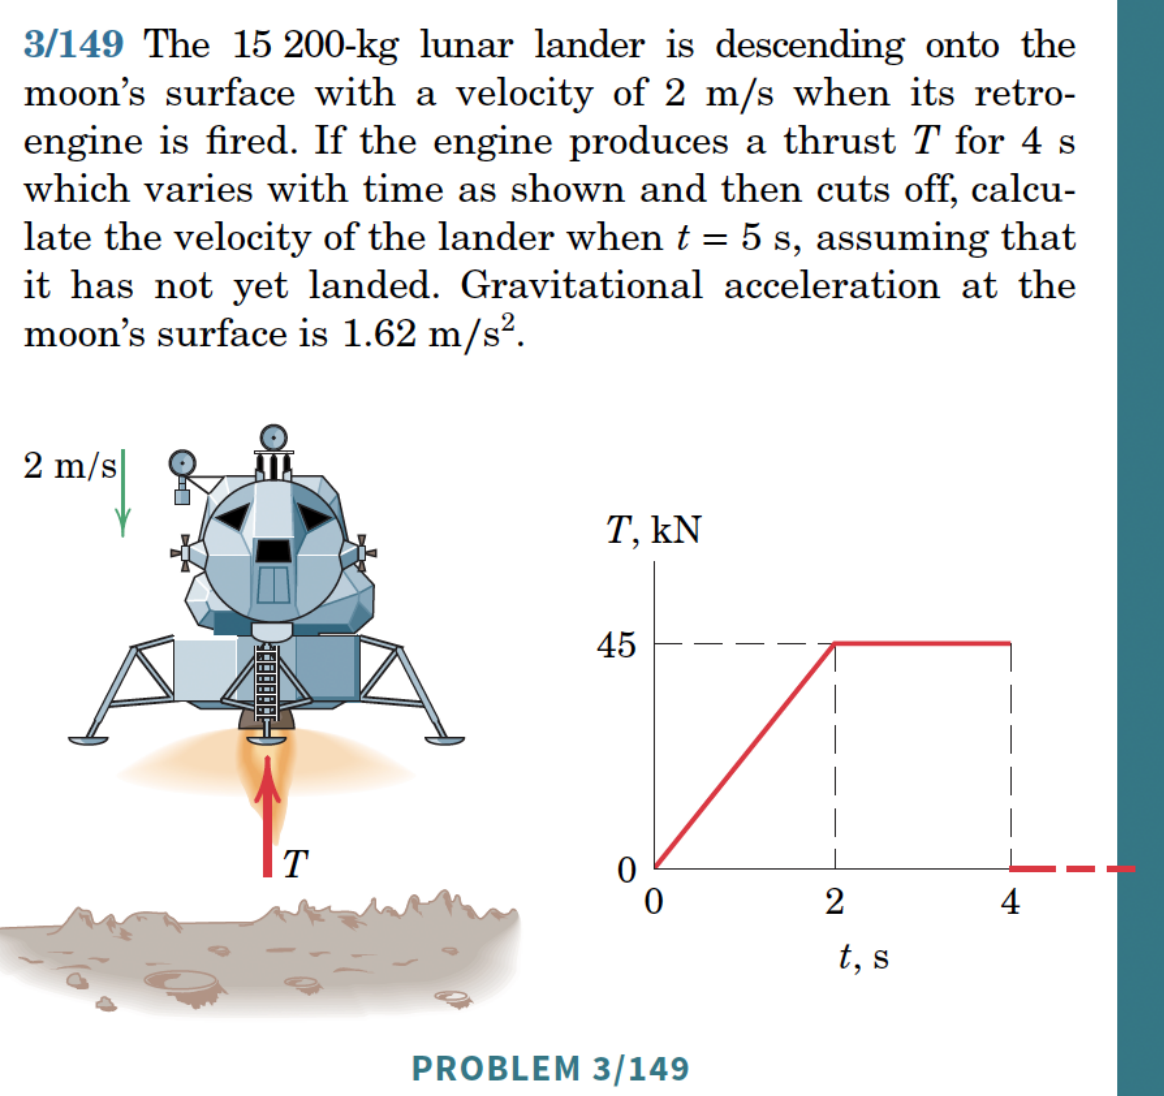
\includegraphics[width=0.5\linewidth,height=\textheight,keepaspectratio]{particle_dynamics/../figures/momenta_and_impulses/03-149.png}

}

\caption{MKB 03-149.}

\end{figure}%

\textbf{2.} {[}MKB 03-159{]} The block is subjected to a time-varying
force \(P(t)\) shown in the plot; \(P=0\) for \(t>3\) s. \emph{(ans.
\(t_s=3.69\) s)}

\begin{figure}[H]

{\centering 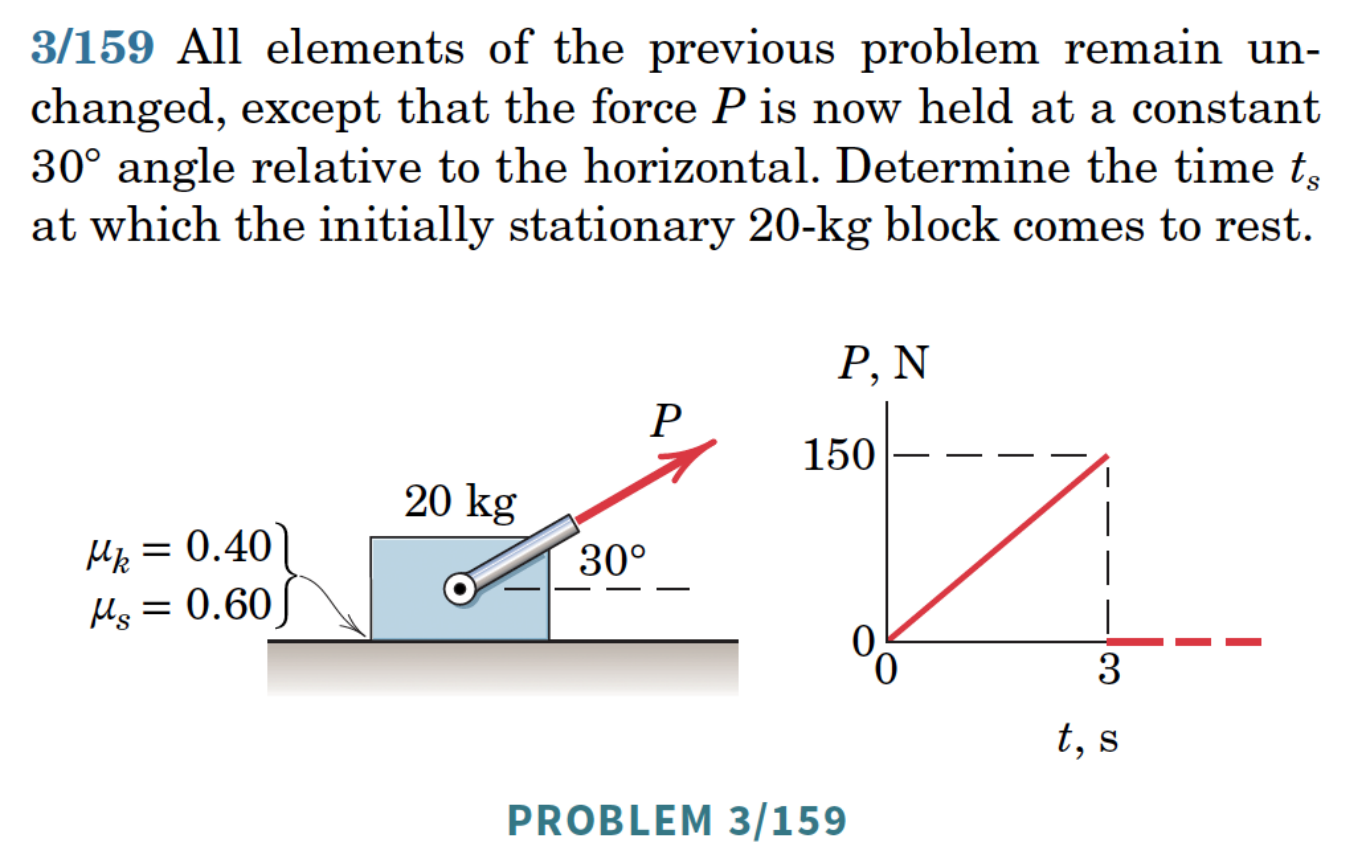
\includegraphics[width=0.5\linewidth,height=\textheight,keepaspectratio]{particle_dynamics/../figures/momenta_and_impulses/03-159.png}

}

\caption{MKB 03-159.}

\end{figure}%

\url{https://youtu.be/ugj4fefUN4c}

\textbf{3.} {[}MKB 03-161{]} Use Newton's third law. Recall
\(\int_{x_A}^{x_B}f(x)\,dx = F_{\mathrm{avg}}(x_B-x_A)\). \emph{(ans.
\(v_f=0.00264\) m/s, \(F_{\mathrm{avg}}=59.5\) N)}

\begin{figure}[H]

{\centering 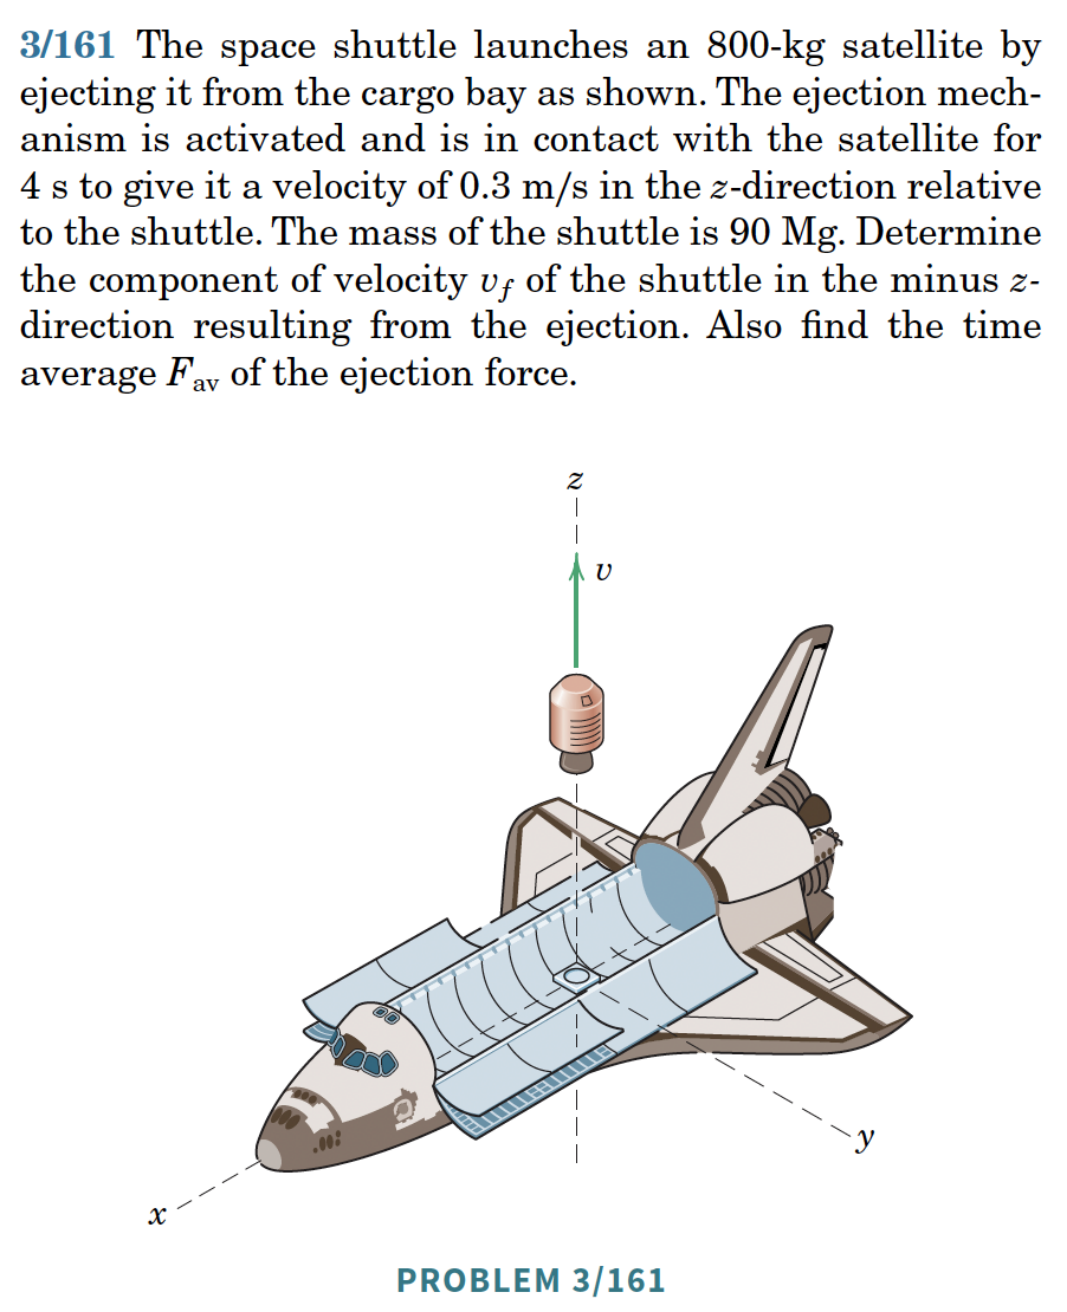
\includegraphics[width=0.5\linewidth,height=\textheight,keepaspectratio]{particle_dynamics/../figures/momenta_and_impulses/03-161.png}

}

\caption{MKB 03-161.}

\end{figure}%

\url{https://youtu.be/Q-F7ew3jFuQ}

\textbf{4.} {[}03-167{]} \emph{(ans. \(R_x=559\) lb, \(R_y=218\) lb)}

\begin{figure}[H]

{\centering 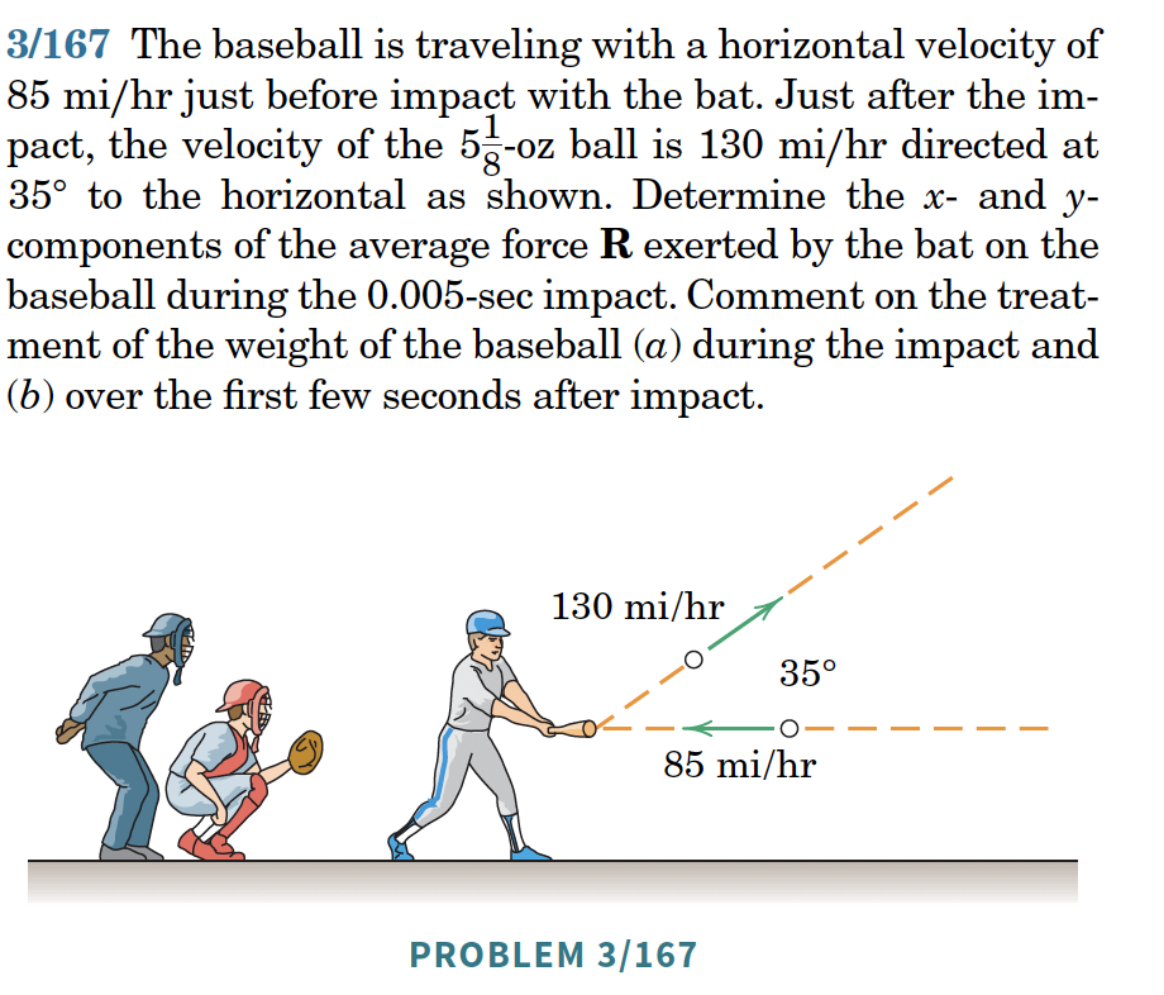
\includegraphics[width=0.5\linewidth,height=\textheight,keepaspectratio]{particle_dynamics/../figures/momenta_and_impulses/03-167.png}

}

\caption{MKB 03-167.}

\end{figure}%

\textbf{5.} {[}03-177{]} Central force problem -- what quantities are
conserved? \emph{(ans. \(v_P=17\,723\) mi/hr)}

\begin{figure}[H]

{\centering 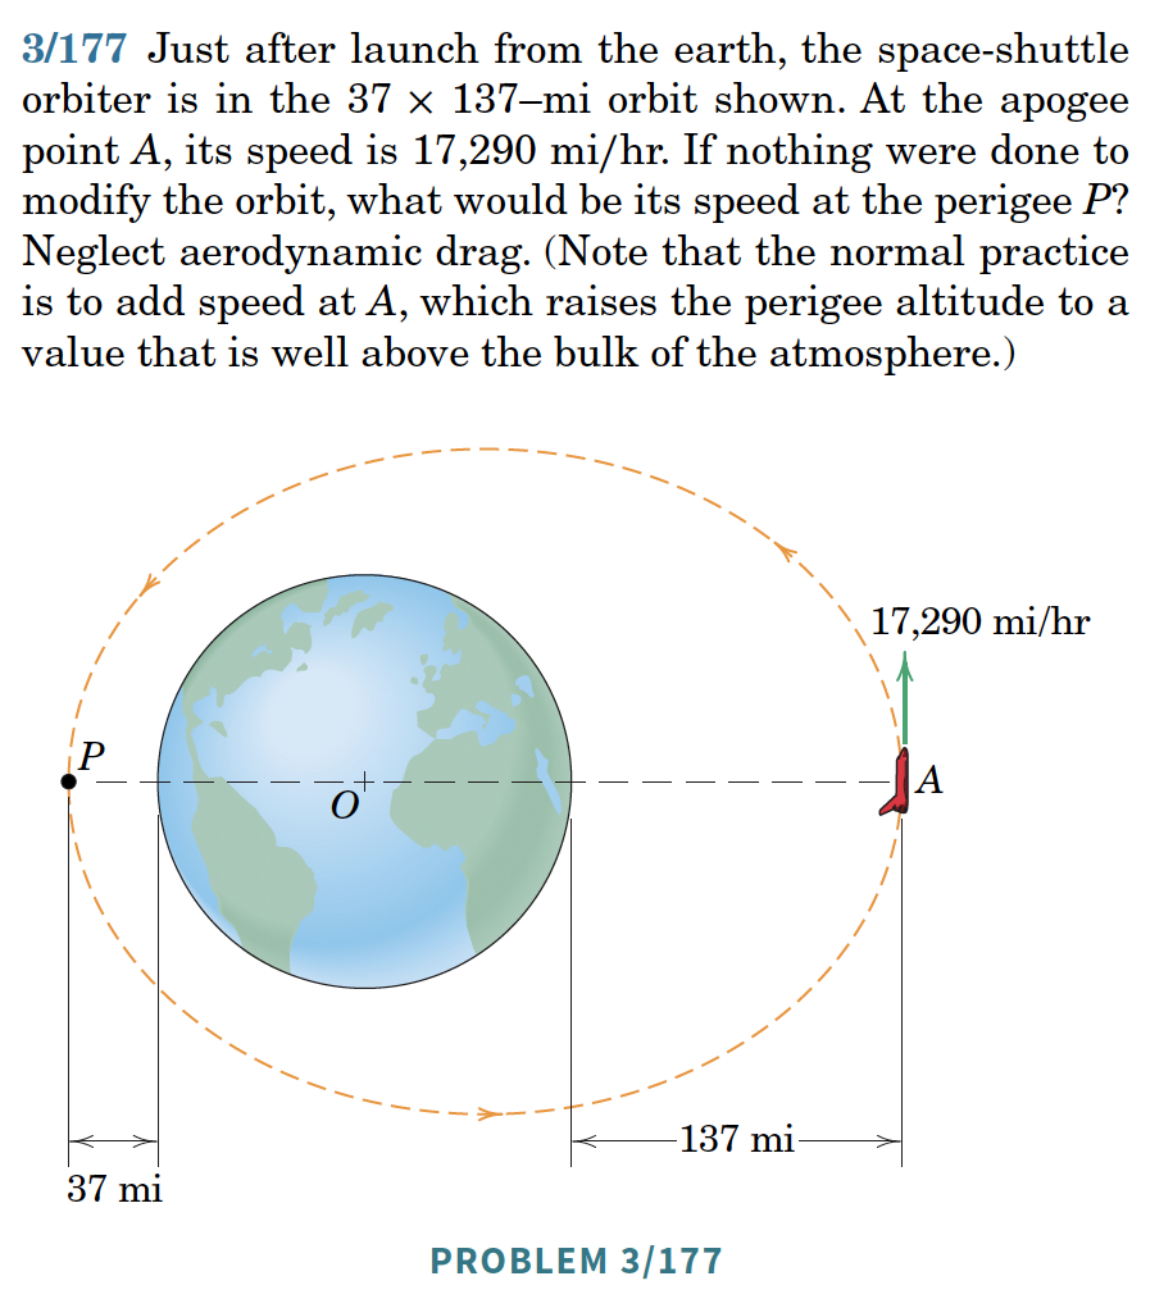
\includegraphics[width=0.5\linewidth,height=\textheight,keepaspectratio]{particle_dynamics/../figures/momenta_and_impulses/03-177.png}

}

\caption{MKB 03-177.}

\end{figure}%

\textbf{6.} {[}03-185{]} \emph{(ans. \(v_B=5.43\) m/s)}

\begin{figure}[H]

{\centering 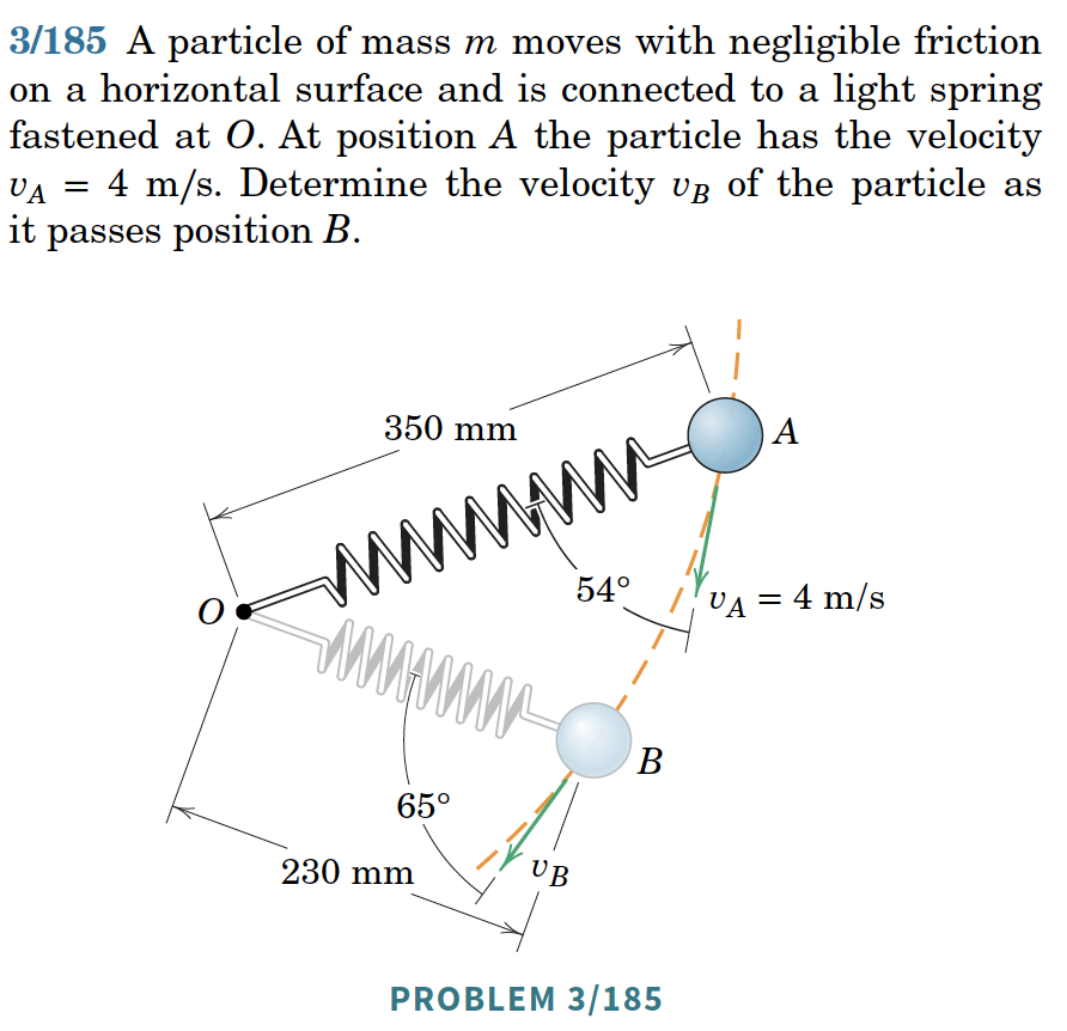
\includegraphics[width=0.5\linewidth,height=\textheight,keepaspectratio]{particle_dynamics/../figures/momenta_and_impulses/03-185.png}

}

\caption{MKB 03-185.}

\end{figure}%

\url{https://youtu.be/V3ussTTlrs8}

\textbf{7.} {[}03-181{]} \emph{(ans. \(|H|=389\) N·m·s, \(|M|=260\)
N·m)}

\textbf{8.} {[}03-192{]} Label \(r\) as \(R\) and the requested angle
\(\theta\) as \(\beta\). The particle moves on a surface of revolution
\(z^2+(r-1.15R)^2=R^2\). Use conservation of total energy and
\(\mathbf{E}_z\)-component of \(\mathbf{H}^O\). \emph{(ans.
\(\theta=52.9^\circ\))}

\begin{figure}[H]

{\centering 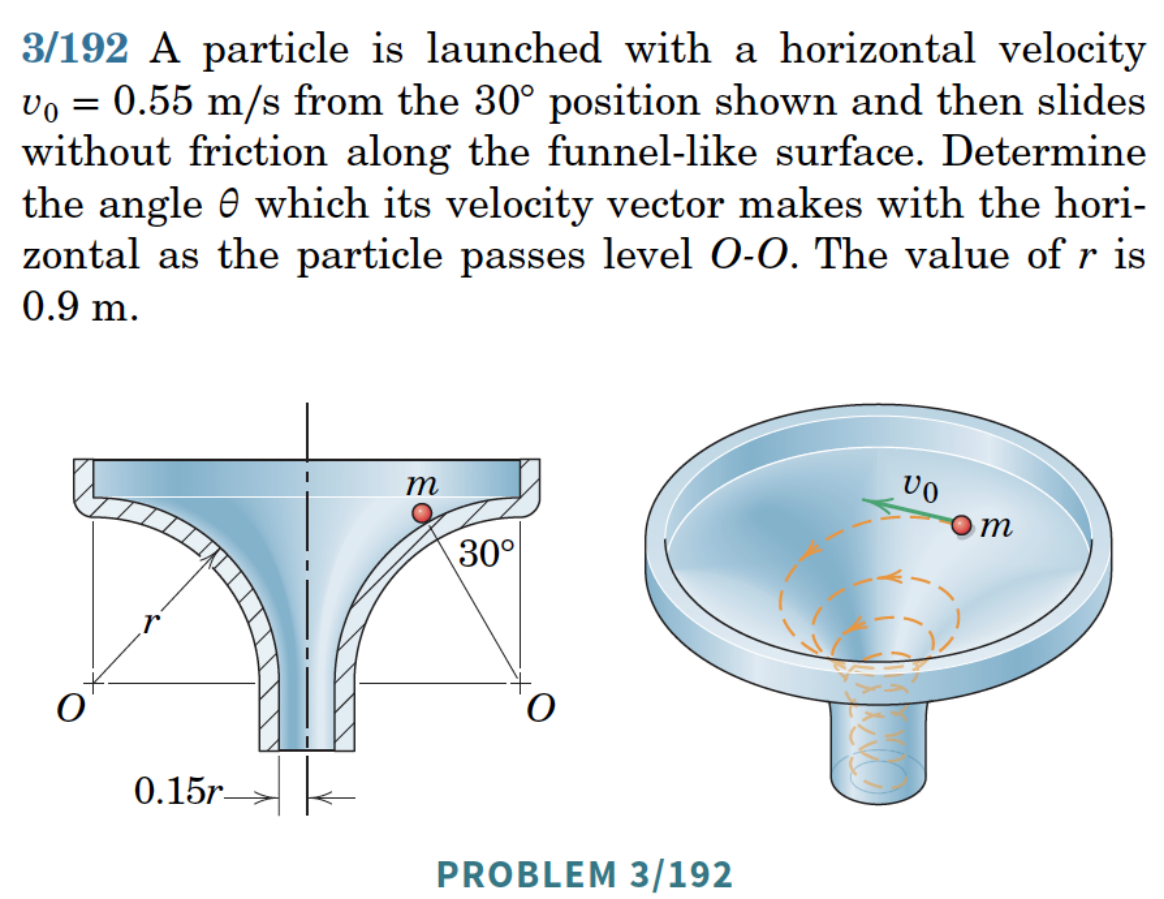
\includegraphics[width=0.5\linewidth,height=\textheight,keepaspectratio]{particle_dynamics/../figures/momenta_and_impulses/03-192.png}

}

\caption{MKB 03-192.}

\end{figure}%

\url{https://youtu.be/jjHTcoIAQmY}

\chapter{Collisions}\label{collisions}

\section{Collision of Two Bodies}\label{collision-of-two-bodies}

\begin{tcolorbox}[enhanced jigsaw, arc=.35mm, bottomrule=.15mm, bottomtitle=1mm, breakable, colback=white, colbacktitle=quarto-callout-tip-color!10!white, colframe=quarto-callout-tip-color-frame, coltitle=black, left=2mm, leftrule=.75mm, opacityback=0, opacitybacktitle=0.6, rightrule=.15mm, title=\textcolor{quarto-callout-tip-color}{\faLightbulb}\hspace{0.5em}{Think!}, titlerule=0mm, toprule=.15mm, toptitle=1mm]

\textbf{Question:} What happens in reality when two cars collide?

\begin{quote}
\textbf{Answer}

In reality, colliding bodies deform --- possibly permanently --- and
their rotational inertia may change.
\end{quote}

\end{tcolorbox}

Ignoring rotational motion, the simplest model uses a mass particle for
each body. Since particles do not deform, we introduce the
\textbf{coefficient of restitution} \(e\).

\section{Frictionless, Oblique, Central Impact of Two
Bodies}\label{frictionless-oblique-central-impact-of-two-bodies}

\begin{figure}[H]

{\centering 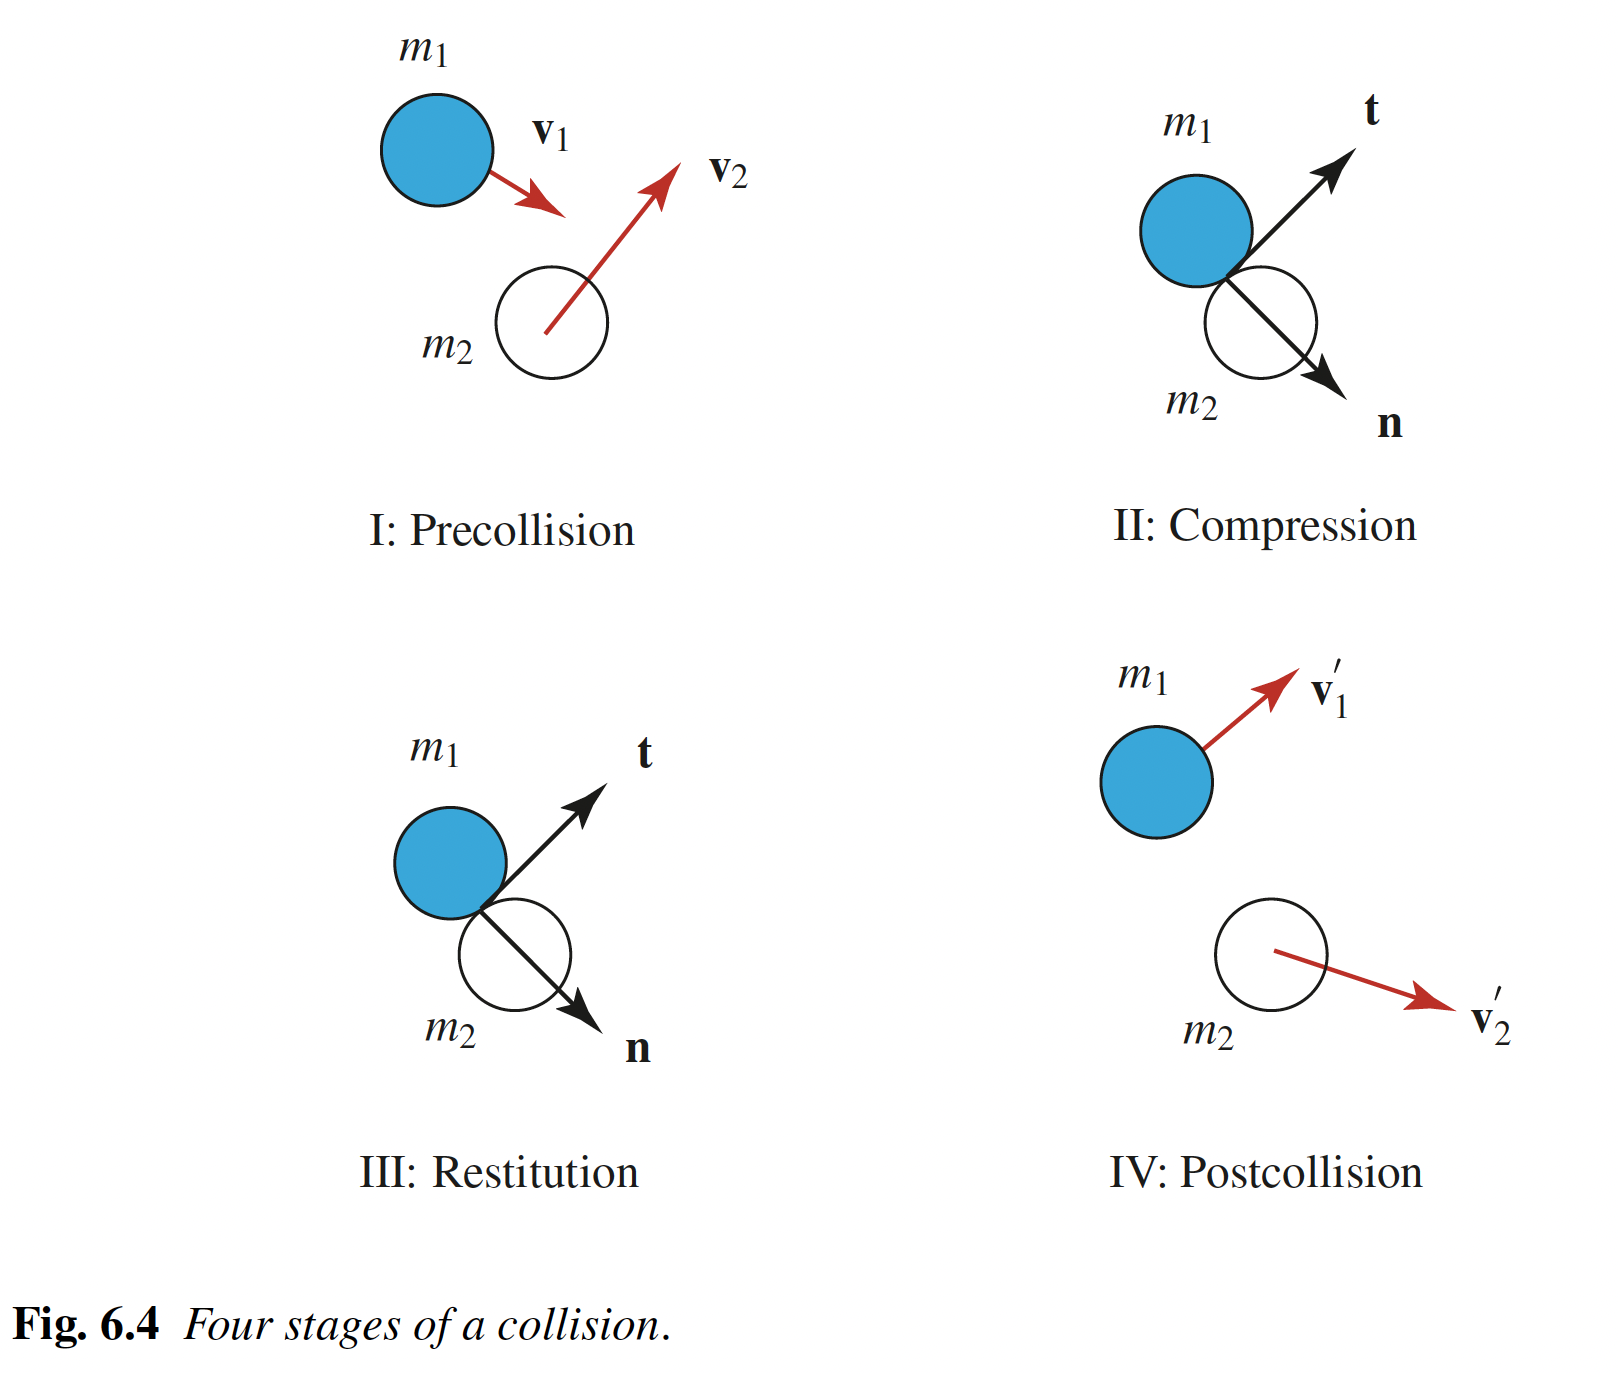
\includegraphics[width=0.5\linewidth,height=\textheight,keepaspectratio]{particle_dynamics/../figures/collisions/collision-stages.png}

}

\caption{Figure from O. M. O'Reilly's Dynamics Primer}

\end{figure}%

\subsection{Assumptions}\label{assumptions}

\begin{itemize}
\tightlist
\item
  Model each body as a mass particle.
\item
  We ignore the rotational inertias of bodies (purely translational
  motion).
\item
  As the bodies are in a state of purely translational motion, all the
  points on the body have the same velocity.
\item
  The position vector of the mass particle is defined to coincide with
  the center of mass of the body it models.
\item
  No friction between particles during collision --- all impact forces
  are along \({\bf n}\).
\item
  The duration of compression (\(t_1-t_0\)) and restitution
  (\(t_2-t_1\)) are very small.
\item
  At time \(t_1\), both particles have the same velocity along
  \({\bf n}\): \(v_{II}\).
\item
  \({\bf F}_{1C} = -{\bf F}_{2C}\), \({\bf F}_{1R} = -{\bf F}_{2R}\).
\end{itemize}

\subsection{Impact Stages}\label{impact-stages}

Let \({\bf n}\) be the common unit normal between the bodies when they
collide. This vector is normal to the lateral surfaces of both bodies at
the unique point of contact. Define a set of orthonormal vectors
\(\{{\bf n},{\bf t}_1,{\bf t}_2\}\) by selecting \({\bf t}_1\) and
\({\bf t}_2\) to be unit tangent vectors to the lateral surface of both
bodies at the point of contact. The impact is assumed to be such that
these vectors are constant for the duration of the impact. At the end of
stage II, the velocities of the bodies in the direction of \({\bf n}\)
are assumed to be equal \((=v_{II})\).

\subsection{Linear Impulses During
Impact}\label{linear-impulses-during-impact}

\begin{tcolorbox}[enhanced jigsaw, arc=.35mm, bottomrule=.15mm, bottomtitle=1mm, breakable, colback=white, colbacktitle=quarto-callout-tip-color!10!white, colframe=quarto-callout-tip-color-frame, coltitle=black, left=2mm, leftrule=.75mm, opacityback=0, opacitybacktitle=0.6, rightrule=.15mm, title=\textcolor{quarto-callout-tip-color}{\faLightbulb}\hspace{0.5em}{Think!}, titlerule=0mm, toprule=.15mm, toptitle=1mm]

\textbf{Question:} Draw the FBDs of \(m_1\) and \(m_2\) separately
during compression and restitution.

\begin{quote}
\textbf{Answer}

\begin{itemize}
\tightlist
\item
  \({\bf F}_{1_d} = F_{1_d}{\bf n}\): force exerted by body 2 on body 1
  during compression.
\item
  \({\bf F}_{1_r} = F_{1_r}{\bf n}\): force exerted by body 2 on body 1
  during restitution.
\item
  \({\bf F}_{2_d}\), \({\bf F}_{2_r}\): reaction forces by body 1 on
  body 2.
\item
  All other forces have resultants \({\bf R}_1\) and \({\bf R}_2\).
\end{itemize}
\end{quote}

\end{tcolorbox}

Since the collision duration is very small, the impulses of
\({\bf R}_1\) and \({\bf R}_2\) vanish. Define the time instants:

\begin{itemize}
\tightlist
\item
  \(t_0\): time just before collision
\item
  \(t_1\): time at the end of compression
\item
  \(t_2\): time at the end of restitution
\end{itemize}

Approximating: \begin{align}
    \begin{split}
        & \int_{t_0}^{t_1}\lp{\bf F}_{1_d}(\tau)+{\bf R}_1(\tau)\rp d\tau \approx \int_{t_0}^{t_1}{\bf F}_{1_d}(\tau)\,d\tau,\\
        & \int_{t_1}^{t_2}\lp{\bf F}_{1_r}(\tau)+{\bf R}_1(\tau)\rp d\tau \approx \int_{t_1}^{t_2}{\bf F}_{1_r}(\tau)\,d\tau,\\
        & \int_{t_0}^{t_1}\lp{\bf F}_{2_d}(\tau)+{\bf R}_2(\tau)\rp d\tau \approx \int_{t_0}^{t_1}{\bf F}_{2_d}(\tau)\,d\tau,\\
        & \int_{t_1}^{t_2}\lp{\bf F}_{2_r}(\tau)+{\bf R}_2(\tau)\rp d\tau \approx \int_{t_1}^{t_2}{\bf F}_{2_r}(\tau)\,d\tau.
    \end{split}
\end{align}

We assume equal and opposite collisional forces: \begin{align}
    \begin{split}
        & {\bf F}_{1_r} = -{\bf F}_{2_r},\\
        & {\bf F}_{1_d} = -{\bf F}_{2_d}.
    \end{split}
\end{align}

We now define the \textbf{coefficient of restitution}: \begin{align}
    e = \frac{\int_{t_1}^{t_2}{\bf F}_{1_r}(\tau)\cdot{\bf n}\,d\tau}{\int_{t_0}^{t_1}{\bf F}_{1_d}(\tau)\cdot{\bf n}\,d\tau} = \frac{\int_{t_1}^{t_2}{\bf F}_{2_r}(\tau)\cdot{\bf n}\,d\tau}{\int_{t_0}^{t_1}{\bf F}_{2_d}(\tau)\cdot{\bf n}\,d\tau}.
\end{align}

\begin{tcolorbox}[enhanced jigsaw, arc=.35mm, bottomrule=.15mm, bottomtitle=1mm, breakable, colback=white, colbacktitle=quarto-callout-tip-color!10!white, colframe=quarto-callout-tip-color-frame, coltitle=black, left=2mm, leftrule=.75mm, opacityback=0, opacitybacktitle=0.6, rightrule=.15mm, title=\textcolor{quarto-callout-tip-color}{\faLightbulb}\hspace{0.5em}{Think!}, titlerule=0mm, toprule=.15mm, toptitle=1mm]

\textbf{Question:} What does \(e=0\) and \(e=1\) mean?

\begin{quote}
\textbf{Answer}

\begin{itemize}
\tightlist
\item
  \(e=1\): perfectly \textbf{elastic} collision --- compression impulse
  equals restitution impulse.
\item
  \(e=0\): perfectly \textbf{plastic} collision --- no restitution
  impulse.
\item
  In general \(0\leq e\leq 1\), determined experimentally.
\end{itemize}
\end{quote}

\end{tcolorbox}

\subsection{The Coefficient of Restitution in Terms of
Velocities}\label{the-coefficient-of-restitution-in-terms-of-velocities}

To write the coefficient of restitution in a more convenient form using
velocities, we first write the linear impulse-linear momentum equations.

\begin{tcolorbox}[enhanced jigsaw, arc=.35mm, bottomrule=.15mm, bottomtitle=1mm, breakable, colback=white, colbacktitle=quarto-callout-tip-color!10!white, colframe=quarto-callout-tip-color-frame, coltitle=black, left=2mm, leftrule=.75mm, opacityback=0, opacitybacktitle=0.6, rightrule=.15mm, title=\textcolor{quarto-callout-tip-color}{\faLightbulb}\hspace{0.5em}{Think!}, titlerule=0mm, toprule=.15mm, toptitle=1mm]

\textbf{Question:} For the above impulses, complete the linear
impulse-linear momentum equations.

\begin{quote}
\textbf{Answer}

\begin{align}
    \begin{split}
        & m_1 v_{II} - m_1{\bf v}_1\cdot{\bf n} = \int_{t_0}^{t_1}{\bf F}_{1_d}(\tau)\cdot{\bf n}\,d\tau,\\
        & m_2 v_{II} - m_2{\bf v}_2\cdot{\bf n} = \int_{t_0}^{t_1}{\bf F}_{2_d}(\tau)\cdot{\bf n}\,d\tau,\\
        & m_1{\bf v}_1'\cdot{\bf n}-m_1 v_{II} = \int_{t_1}^{t_2}{\bf F}_{1_r}(\tau)\cdot{\bf n}\,d\tau = e\int_{t_0}^{t_1}{\bf F}_{1_d}(\tau)\cdot{\bf n}\,d\tau,\\
        & m_2{\bf v}_2'\cdot{\bf n}-m_2 v_{II} = \int_{t_1}^{t_2}{\bf F}_{2_r}(\tau)\cdot{\bf n}\,d\tau = e\int_{t_0}^{t_1}{\bf F}_{2_d}(\tau)\cdot{\bf n}\,d\tau.
    \end{split}
\end{align}
\end{quote}

\end{tcolorbox}

From these 4 equations, we can isolate the common velocity \(v_{II}\) of
the particles along \({\bf n}\) at time \(t_1\): \begin{align}
    v_{II} = \frac{{\bf v}_1'\cdot{\bf n}+e{\bf v}_1\cdot{\bf n}}{1+e} = \frac{{\bf v}_2'\cdot{\bf n}+e{\bf v}_2\cdot{\bf n}}{1+e}.
\end{align}

From this, we get the familiar expression for the coefficient of
restitution: \begin{align}
    e = \frac{{\bf v}_2'\cdot{\bf n}-{\bf v}_1'\cdot{\bf n}}{{\bf v}_1\cdot{\bf n}-{\bf v}_2\cdot{\bf n}}.
\end{align}

\url{https://youtu.be/0GcIPJgpwN4}

\begin{tcolorbox}[enhanced jigsaw, arc=.35mm, bottomrule=.15mm, bottomtitle=1mm, breakable, colback=white, colbacktitle=quarto-callout-important-color!10!white, colframe=quarto-callout-important-color-frame, coltitle=black, left=2mm, leftrule=.75mm, opacityback=0, opacitybacktitle=0.6, rightrule=.15mm, title=\textcolor{quarto-callout-important-color}{\faExclamation}\hspace{0.5em}{Note!}, titlerule=0mm, toprule=.15mm, toptitle=1mm]

When one object impacts a massive constrained object (e.g.~a wall), the
velocity of the massive object is unaffected by the collision.

\end{tcolorbox}

\section{Example: The Most General Planar Impact
Problem}\label{example-the-most-general-planar-impact-problem}

\begin{tcolorbox}[enhanced jigsaw, arc=.35mm, bottomrule=.15mm, bottomtitle=1mm, breakable, colback=white, colbacktitle=quarto-callout-warning-color!10!white, colframe=quarto-callout-warning-color-frame, coltitle=black, left=2mm, leftrule=.75mm, opacityback=0, opacitybacktitle=0.6, rightrule=.15mm, title=\textcolor{quarto-callout-warning-color}{\faExclamationTriangle}\hspace{0.5em}{Example}, titlerule=0mm, toprule=.15mm, toptitle=1mm]

\textbf{Question:} Given particles \(m_1\) and \(m_2\) with pre-impact
velocities \({\bf v}_1\) and \({\bf v}_2\), find the post-impact
velocities. The coefficient of restitution \(e\) is given.

\begin{quote}
\textbf{Answer}

There are 4 unknowns (components of \({\bf v}_1'\) and \({\bf v}_2'\)
along \({\bf n}\), \({\bf t}_1\), \({\bf t}_2\)). Along the tangent
directions: velocities are unchanged. Along \({\bf n}\): we have the
conservation of linear momentum and the restitution equation.
\end{quote}

\end{tcolorbox}

\url{https://youtu.be/4zI-bUmKLKI}

\section{Energy Loss During Impact}\label{energy-loss-during-impact}

Pre-impact and post-impact kinetic energies: \begin{align}
    T &= \frac{1}{2}m_1{\bf v}_1\cdot{\bf v}_1+\frac{1}{2}m_2{\bf v}_2\cdot{\bf v}_2,\\
    T' &= \frac{1}{2}m_1{\bf v}_1'\cdot{\bf v}_1'+\frac{1}{2}m_2{\bf v}_2'\cdot{\bf v}_2'.
\end{align}

The energy lost: \begin{align}
    \begin{split}
        T-T' &= \frac{1}{2}m_1\lp({\bf v}_1\cdot{\bf n})^2-({\bf v}_1'\cdot{\bf n})^2\rp+\frac{1}{2}m_2\lp({\bf v}_2\cdot{\bf n})^2-({\bf v}_2'\cdot{\bf n})^2\rp\\
        &= \frac{m_1 m_2}{2(m_1+m_2)}\lp{\bf v}_1\cdot{\bf n}-{\bf v}_2\cdot{\bf n}\rp^2(1-e^2).
    \end{split}
\end{align}

Hence, for \(0\leq e\leq 1\), kinetic energy cannot increase as a result
of impact.

\section{Negative Values of the Coefficient of
Restitution}\label{negative-values-of-the-coefficient-of-restitution}

\begin{tcolorbox}[enhanced jigsaw, arc=.35mm, bottomrule=.15mm, bottomtitle=1mm, breakable, colback=white, colbacktitle=quarto-callout-tip-color!10!white, colframe=quarto-callout-tip-color-frame, coltitle=black, left=2mm, leftrule=.75mm, opacityback=0, opacitybacktitle=0.6, rightrule=.15mm, title=\textcolor{quarto-callout-tip-color}{\faLightbulb}\hspace{0.5em}{Think!}, titlerule=0mm, toprule=.15mm, toptitle=1mm]

\textbf{Question:} What does a negative \(e\) mean for a ball impacting
a wall?

\begin{quote}
\textbf{Answer}

When the coefficient of restitution is negative, \begin{align}
    e = \frac{{\bf v}_2'\cdot{\bf n}-{\bf v}_1'\cdot{\bf n}}{{\bf v}_1\cdot{\bf n}-{\bf v}_2\cdot{\bf n}} \leq 0,
\end{align} and hence \({\bf v}_1'\cdot{\bf n}-{\bf v}_2'\cdot{\bf n}\)
and \({\bf v}_1\cdot{\bf n}-{\bf v}_2\cdot{\bf n}\) have the same sign.
As a result, the colliding bodies pass through each other during the
course of the impact. To eliminate this behavior, it is generally
assumed that \(e\) is positive.
\end{quote}

\end{tcolorbox}

\section{Exercises}\label{exercises-12}

\emph{The following problems are from Set 13 -- Collisions. In all of
the following problems, specify the system you are considering. Are
there any conservations in that system? Remember that the linear
momentum of a system is conserved in a fixed direction if the sum of
forces acting on the system along this direction is zero.}

\textbf{1.} {[}MKB 03-142{]}

\begin{figure}[H]

{\centering 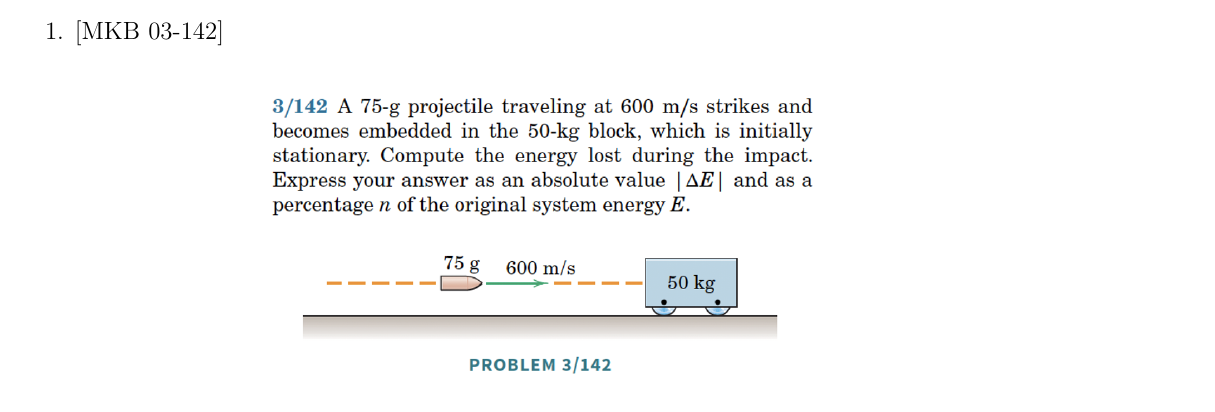
\includegraphics[width=0.5\linewidth,height=\textheight,keepaspectratio]{particle_dynamics/../figures/collisions/problems/03-142.png}

}

\caption{MKB 03-142.}

\end{figure}%

\textbf{2.} {[}MKB 03-196{]}

\begin{figure}[H]

{\centering 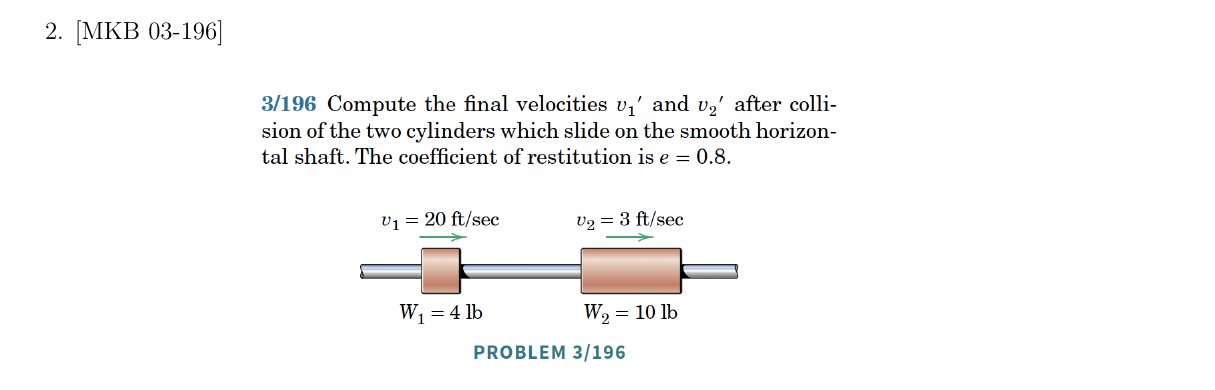
\includegraphics[width=0.5\linewidth,height=\textheight,keepaspectratio]{particle_dynamics/../figures/collisions/problems/03-196.png}

}

\caption{MKB 03-196.}

\end{figure}%

\textbf{3.} {[}MKB 03-197{]}

\begin{figure}[H]

{\centering 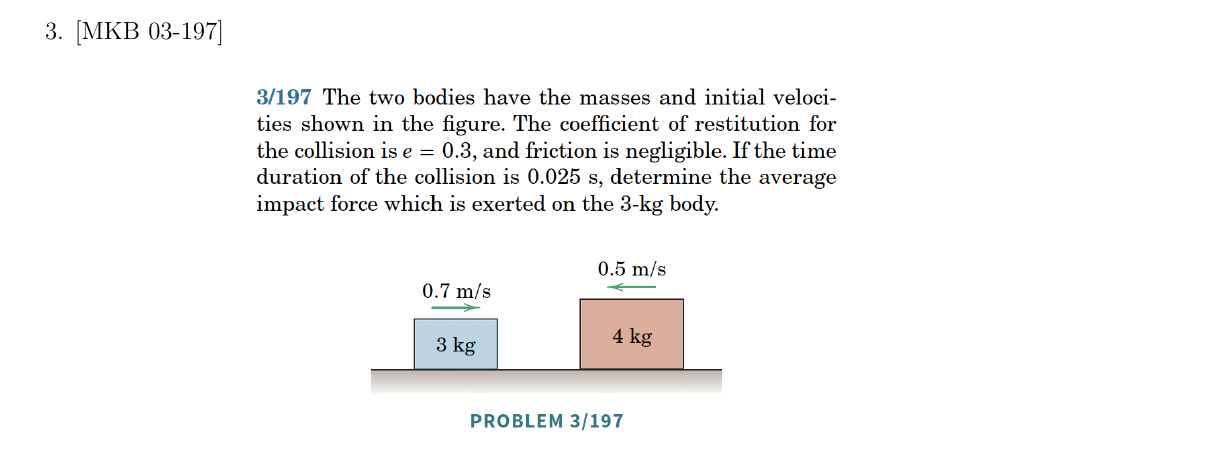
\includegraphics[width=0.5\linewidth,height=\textheight,keepaspectratio]{particle_dynamics/../figures/collisions/problems/03-197.png}

}

\caption{MKB 03-197.}

\end{figure}%

\textbf{4.} {[}03-201{]}

\begin{figure}[H]

{\centering 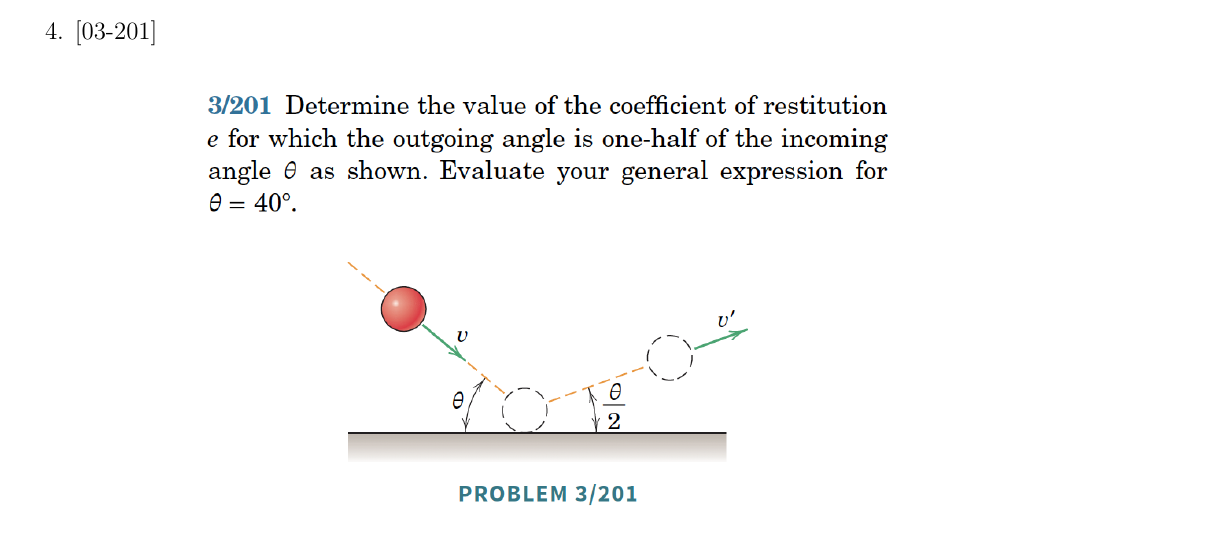
\includegraphics[width=0.5\linewidth,height=\textheight,keepaspectratio]{particle_dynamics/../figures/collisions/problems/03-201.png}

}

\caption{MKB 03-201.}

\end{figure}%

\textbf{5.} {[}03-212{]}

\begin{figure}[H]

{\centering 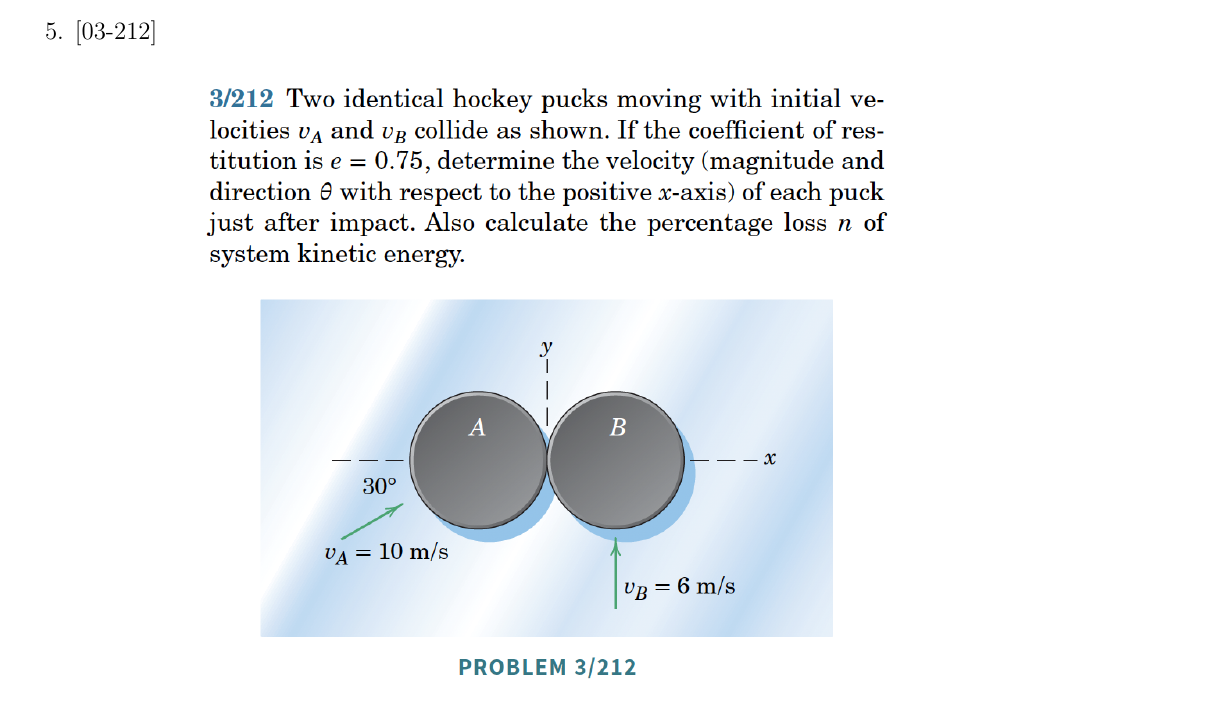
\includegraphics[width=0.5\linewidth,height=\textheight,keepaspectratio]{particle_dynamics/../figures/collisions/problems/03-212.png}

}

\caption{MKB 03-212.}

\end{figure}%

\part{System of Particles}

\chapter{System of Particles}\label{system-of-particles-1}

\begin{center}
\pandocbounded{
\includegraphics[keepaspectratio]{system_of_particles/system_of_particles_files/figure-pdf/unnamed-chunk-1-1.pdf}}
\end{center}

Consider a system of \(n\) particles. A typical particle has mass
\(m_i\), position vector \({\bf r}_i\) relative to \(O\), velocity
\({\bf v}_i = \dot{\bf r}_i,\) acceleration
\({\bf a}_i = \dot{\bf v}_i\), linear momentum
\({\bf G}_i = m_i{\bf v}_i,\) angular momentum relative to some point
\(P\) \({\bf H}^P_i = ({\bf r}_i-{\bf r}_P)\times{\bf G}_i,\) and
kinetic energy \(T_i = \frac{1}{2}m_i{\bf v}_i\cdot{\bf v}_i\).

In this chapter, we define analogous system-level quantities and derive
the balance laws for the system from the balance law for each individual
particle.

\section{Center of Mass}\label{center-of-mass}

\begin{tcolorbox}[enhanced jigsaw, arc=.35mm, bottomrule=.15mm, bottomtitle=1mm, breakable, colback=white, colbacktitle=quarto-callout-tip-color!10!white, colframe=quarto-callout-tip-color-frame, coltitle=black, left=2mm, leftrule=.75mm, opacityback=0, opacitybacktitle=0.6, rightrule=.15mm, title=\textcolor{quarto-callout-tip-color}{\faLightbulb}\hspace{0.5em}{Think!}, titlerule=0mm, toprule=.15mm, toptitle=1mm]

\textbf{Question:} What is the position vector of the center of mass of
a system of particles?

\begin{quote}
\textbf{Answer}

The center of mass \(C\) has position vector \begin{align}
    {\bf r}_C = \frac{1}{m}\sum_{k=1}^n m_k{\bf r}_k,
\end{align} where \(m = \sum_{k=1}^n m_k\) is the total mass.
\end{quote}

\end{tcolorbox}

\begin{tcolorbox}[enhanced jigsaw, arc=.35mm, bottomrule=.15mm, bottomtitle=1mm, breakable, colback=white, colbacktitle=quarto-callout-warning-color!10!white, colframe=quarto-callout-warning-color-frame, coltitle=black, left=2mm, leftrule=.75mm, opacityback=0, opacitybacktitle=0.6, rightrule=.15mm, title=\textcolor{quarto-callout-warning-color}{\faExclamationTriangle}\hspace{0.5em}{Example}, titlerule=0mm, toprule=.15mm, toptitle=1mm]

\textbf{Question:} Consider an unsymmetrical dumbbell: particle 1 of
mass \(m\) and particle 2 of mass \(3m\) connected by a massless rigid
rod, with \begin{align*}
    {\bf r}_1 = {\bf E}_x+{\bf E}_y, \qquad {\bf r}_2 = 2{\bf E}_x.
\end{align*} Calculate \({\bf r}_C\). Is \(C\) located on the dumbbell?

\pandocbounded{
\includegraphics[keepaspectratio]{system_of_particles/system_of_particles_files/figure-pdf/unnamed-chunk-2-1.pdf}}

\begin{quote}
\textbf{Answer}

\begin{align*}
    {\bf r}_C = \frac{m{\bf r}_1+3m{\bf r}_2}{m+3m} = \frac{{\bf r}_1+3{\bf r}_2}{4} = \frac{7}{4}{\bf E}_x+\frac{1}{4}{\bf E}_y.
\end{align*} We can check mathematically that \(C\) lies on the line
connecting \(m_1\) and \(m_2\) by calculating the equation of that line
and checking at \(C\) belongs to it.

Alternatively, we can define a new basis, \(\{{\bf u},{\bf v}\}\) and
calculate the position of \(C\) relative to \(m_1\) on that basis. This
should be along \({\bf u}\).
\end{quote}

\end{tcolorbox}

Note the useful identity: relative to any reference point \(A\),
\begin{align}
    {\bf r}_{C/A} = \frac{\sum_i m_i{\bf r}_{i/A}}{\sum_i m_i}.
\end{align}

\begin{tcolorbox}[enhanced jigsaw, arc=.35mm, bottomrule=.15mm, bottomtitle=1mm, breakable, colback=white, colbacktitle=quarto-callout-tip-color!10!white, colframe=quarto-callout-tip-color-frame, coltitle=black, left=2mm, leftrule=.75mm, opacityback=0, opacitybacktitle=0.6, rightrule=.15mm, title=\textcolor{quarto-callout-tip-color}{\faLightbulb}\hspace{0.5em}{Think!}, titlerule=0mm, toprule=.15mm, toptitle=1mm]

\textbf{Question:} Show that
\(\sum_{k=1}^n m_k({\bf r}_C-{\bf r}_k) = {\bf 0}\) and
\(\sum_{k=1}^n m_k({\bf v}_C-{\bf v}_k) = {\bf 0}\).

\begin{quote}
\textbf{Answer}

Both follow directly from the definition of the center of mass.
\end{quote}

\end{tcolorbox}

Differentiating the position of the center of mass: \begin{align}
    {\bf v}_C = \frac{1}{m}\sum_{k=1}^n m_k{\bf v}_k = \frac{1}{m}\sum_{k=1}^n{\bf G}_k.
\end{align} Notice that the velocity of the center of mass is the
weighted sum of the velocities of the particles.

\begin{tcolorbox}[enhanced jigsaw, arc=.35mm, bottomrule=.15mm, bottomtitle=1mm, breakable, colback=white, colbacktitle=quarto-callout-tip-color!10!white, colframe=quarto-callout-tip-color-frame, coltitle=black, left=2mm, leftrule=.75mm, opacityback=0, opacitybacktitle=0.6, rightrule=.15mm, title=\textcolor{quarto-callout-tip-color}{\faLightbulb}\hspace{0.5em}{Think!}, titlerule=0mm, toprule=.15mm, toptitle=1mm]

\textbf{Question:} Show that
\(\sum_{k=1}^nm_k({\bf r}_C-{\bf r}_k) = {\bf 0}\) and
\(\sum_{k=1}^nm_k({\bf v}_C-{\bf v}_k) = {\bf 0}\).

\begin{quote}
\textbf{Answer}

\ldots{}
\end{quote}

\end{tcolorbox}

\section{Linear Momentum}\label{linear-momentum}

The linear momentum of the system is \begin{align}
    {\bf G} = m\frac{d{\bf r}}{dt} = \sum_{k=1}^n m_k\frac{d{\bf r}_k}{dt} = \sum_{k=1}^n{\bf G}_k.
\end{align} The linear momentum of the system equals that of its center
of mass.

\section{Angular Momentum}\label{angular-momentum}

The angular momentum \({\bf H}^P\) of the system of particles relative
to a point \(P\), whose position vector relative to \(O\) is
\({\bf r}_P\), is the sum of the individual angular momenta:
\begin{align}
    {\bf H}^P = \sum_{k=1}^n{\bf H}^{P_K} = \sum_{k=1}^n({\bf r}_k-{\bf r}_P)\times m_k{\bf v}_k = {\bf H}^C+({\bf r}_C-{\bf r}_P)\times{\bf G},
\end{align} where \begin{align}
    {\bf H}^C = \sum_{k=1}^n({\bf r}_k-{\bf r}_C)\times m_k{\bf v}_k = \sum_{k=1}^n({\bf r}_k-{\bf r}_C)\times m_k({\bf v}_k-{\bf v}_C).
\end{align}

\begin{tcolorbox}[enhanced jigsaw, arc=.35mm, bottomrule=.15mm, bottomtitle=1mm, breakable, colback=white, colbacktitle=quarto-callout-tip-color!10!white, colframe=quarto-callout-tip-color-frame, coltitle=black, left=2mm, leftrule=.75mm, opacityback=0, opacitybacktitle=0.6, rightrule=.15mm, title=\textcolor{quarto-callout-tip-color}{\faLightbulb}\hspace{0.5em}{Think!}, titlerule=0mm, toprule=.15mm, toptitle=1mm]

\textbf{Question:} Show that
\(\sum_{k=1}^n({\bf r}_k-{\bf r}_P)\times m_k{\bf v}_k = {\bf H}^C+({\bf r}_C-{\bf r}_P)\times{\bf G}\).

\begin{quote}
\textbf{Answer}

Introduce \({\bf r}_C-{\bf r}_C\) inside the sum and expand.
\end{quote}

\end{tcolorbox}

\section{Kinetic Energy}\label{kinetic-energy-1}

The kinetic energy of the system is: \begin{align}
    T = \sum_{k=1}^n\frac{1}{2}m_k{\bf v}_k\cdot{\bf v}_k = \frac{1}{2}m{\bf v}_C\cdot{\bf v}_C+\frac{1}{2}\sum_{k=1}^n m_k({\bf v}_k-{\bf v}_C)\cdot({\bf v}_k-{\bf v}_C).
\end{align} The kinetic energy splits into the kinetic energy of the
center of mass plus the kinetic energy relative to the center of mass.
In general, \(T \neq \frac{1}{2}m{\bf v}_C\cdot{\bf v}_C\).

\begin{tcolorbox}[enhanced jigsaw, arc=.35mm, bottomrule=.15mm, bottomtitle=1mm, breakable, colback=white, colbacktitle=quarto-callout-tip-color!10!white, colframe=quarto-callout-tip-color-frame, coltitle=black, left=2mm, leftrule=.75mm, opacityback=0, opacitybacktitle=0.6, rightrule=.15mm, title=\textcolor{quarto-callout-tip-color}{\faLightbulb}\hspace{0.5em}{Think!}, titlerule=0mm, toprule=.15mm, toptitle=1mm]

\textbf{Question:} Prove
\(\sum_{k=1}^n\frac{1}{2}m_k{\bf v}_k\cdot{\bf v}_k = \frac{1}{2}m{\bf v}_C\cdot{\bf v}_C+\frac{1}{2}\sum_{k=1}^n m_k({\bf v}_k-{\bf v}_C)\cdot({\bf v}_k-{\bf v}_C)\).

\begin{quote}
\textbf{Answer}

Add \({\bf v}_C-{\bf v}_C\) to each \({\bf v}_k\), expand, and use
\(\sum m_k({\bf v}_k-{\bf v}_C) = {\bf 0}\).
\end{quote}

\end{tcolorbox}

\section{Kinetics: Balance of Linear
Momentum}\label{kinetics-balance-of-linear-momentum}

Starting from \({\bf F}_i = m_i{\bf a}_i\) for each particle and
summing: \begin{align}
    {\bf F} = \sum_{k=1}^n{\bf F}_k = m{\bf a}_C.
\end{align} The resultant external force equals the total mass times the
acceleration of the center of mass.

\begin{tcolorbox}[enhanced jigsaw, arc=.35mm, bottomrule=.15mm, bottomtitle=1mm, breakable, colback=white, colbacktitle=quarto-callout-important-color!10!white, colframe=quarto-callout-important-color-frame, coltitle=black, left=2mm, leftrule=.75mm, opacityback=0, opacitybacktitle=0.6, rightrule=.15mm, title=\textcolor{quarto-callout-important-color}{\faExclamation}\hspace{0.5em}{Note!}, titlerule=0mm, toprule=.15mm, toptitle=1mm]

The conditions for conservation of linear momentum of a system
(completely or along a direction) are analogous to those for a single
particle: \({\bf F}\cdot{\bf c} = 0\) for a constant \({\bf c}\).

\end{tcolorbox}

\section{Kinetics: Balance of Angular
Momentum}\label{kinetics-balance-of-angular-momentum}

Starting from
\({\bf H}^P = \sum_{k=1}^n({\bf r}_k-{\bf r}_P)\times m_k{\bf v}_k\),
the time derivative is: \begin{align}
    \dot{\bf H}^P = \sum_{k=1}^n({\bf r}_k-{\bf r}_P)\times{\bf F}_k-{\bf v}_P\times{\bf G} = {\bf M}^P-{\bf v}_P\times{\bf G},
\end{align} where the resultant moment of the system of forces relative
to \(P\) is
\({\bf M}^P = \sum_{k=1}^n({\bf r}_k-{\bf r}_P)\times{\bf F}_k\). The
angular momentum theorem becomes \begin{align}
    \dot{\bf H}^P = {\bf M}^P-{\bf v}_P\times{\bf G}.
\end{align}

\begin{tcolorbox}[enhanced jigsaw, arc=.35mm, bottomrule=.15mm, bottomtitle=1mm, breakable, colback=white, colbacktitle=quarto-callout-important-color!10!white, colframe=quarto-callout-important-color-frame, coltitle=black, left=2mm, leftrule=.75mm, opacityback=0, opacitybacktitle=0.6, rightrule=.15mm, title=\textcolor{quarto-callout-important-color}{\faExclamation}\hspace{0.5em}{Note!}, titlerule=0mm, toprule=.15mm, toptitle=1mm]

\(\dot{\bf H}^P\) is \textbf{not} necessarily equal to \({\bf M}^P\).
The two agree only in special cases.

\end{tcolorbox}

Two important special cases:

\begin{enumerate}
\def\labelenumi{\arabic{enumi}.}
\tightlist
\item
  \(P = O\) (fixed origin, \({\bf v}_O = {\bf 0}\)):
  \(\dot{\bf H}^O = {\bf M}^O = \sum_{k=1}^n{\bf r}_k\times{\bf F}_k\).
\item
  \(P = C\) (center of mass, \({\bf v}_C\times{\bf G} = {\bf 0}\)):
  \(\dot{\bf H}^C = {\bf M}^C = \sum_{k=1}^n({\bf r}_k-{\bf r}_C)\times{\bf F}_k\).
\end{enumerate}

\begin{tcolorbox}[enhanced jigsaw, arc=.35mm, bottomrule=.15mm, bottomtitle=1mm, breakable, colback=white, colbacktitle=quarto-callout-important-color!10!white, colframe=quarto-callout-important-color-frame, coltitle=black, left=2mm, leftrule=.75mm, opacityback=0, opacitybacktitle=0.6, rightrule=.15mm, title=\textcolor{quarto-callout-important-color}{\faExclamation}\hspace{0.5em}{Note!}, titlerule=0mm, toprule=.15mm, toptitle=1mm]

The conditions for conservation of angular momentum of a system are
analogous to those for a single particle.

\end{tcolorbox}

\emph{Example: A pendulum suspended from a cart on smooth horizontal
rails --- write the BoAM in 3 forms.}

\section{Work-Energy Theorem}\label{work-energy-theorem}

The work-energy theorem for a system of particles is: \begin{align}
    \dot{T} = \sum_{k=1}^n{\bf F}_k\cdot{\bf v}_k,
\end{align} and \begin{align}
    \dot{E} = \sum_{k=1}^n{\bf F}_{nc_k}\cdot{\bf v}_k.
\end{align} where \({\bf F}_{nc_k}\) is the nonconservative force acting
on the \(k\)th particle and \(E\) is the total energy of the system of
particles. Integrating: \begin{align}
    T(t_2)-T(t_1) = \sum_{k=1}^n W_{{\bf F}_k,12}, \qquad W_{{\bf F}_k,12} = \int_{t_1}^{t_2}{\bf F}_k\cdot{\bf v}_k\,dt.
\end{align}

\begin{tcolorbox}[enhanced jigsaw, arc=.35mm, bottomrule=.15mm, bottomtitle=1mm, breakable, colback=white, colbacktitle=quarto-callout-important-color!10!white, colframe=quarto-callout-important-color-frame, coltitle=black, left=2mm, leftrule=.75mm, opacityback=0, opacitybacktitle=0.6, rightrule=.15mm, title=\textcolor{quarto-callout-important-color}{\faExclamation}\hspace{0.5em}{Note!}, titlerule=0mm, toprule=.15mm, toptitle=1mm]

The work of a force is the integral of the force dotted with the
velocity of the \textbf{point of application} of the force.

\end{tcolorbox}

\begin{tcolorbox}[enhanced jigsaw, arc=.35mm, bottomrule=.15mm, bottomtitle=1mm, breakable, colback=white, colbacktitle=quarto-callout-warning-color!10!white, colframe=quarto-callout-warning-color-frame, coltitle=black, left=2mm, leftrule=.75mm, opacityback=0, opacitybacktitle=0.6, rightrule=.15mm, title=\textcolor{quarto-callout-warning-color}{\faExclamationTriangle}\hspace{0.5em}{Example}, titlerule=0mm, toprule=.15mm, toptitle=1mm]

\textbf{Question:} Consider the unsymmetrical dumbbell (particle 1 of
mass \(m\), particle 2 of mass \(3m\), massless rod) moving in the
smooth \(\{{\bf E}_x,{\bf E}_y\}\) plane with gravity along
\(-{\bf E}_z\). Is the energy conserved?

\begin{quote}
\textbf{Answer}

Drawing the FBDs of both masses: \ldots{}
\end{quote}

\end{tcolorbox}

\section{Summary}\label{summary-10}

\textbf{Kinematics of a system of particles}

Consider a system of \(n\) particles each with mass \(m_i\) and with
position vector \({\bf r}_i\) from the origin. The total mass of the
system of particles is \(m = \sum_{i=1}^n m_i\). The center of mass of
the system of particles \(C\) is defined to be located at \begin{align}
    {\bf r}_C = \frac{\sum_{i=1}^n m_i{\bf r}_i}{m}.
\end{align} The velocity and acceleration of the center of mass are then
obtained by differentiation \({\bf r}_C\). \begin{align}
    {\bf v}_C = \frac{\sum_{i=1}^n m_i{\bf v}_i}{m},\quad\text{and}\quad{\bf a}_C = \frac{\sum_{i=1}^n m_i{\bf a}_i}{m}.
\end{align} The linear momentum of a system of particles is the sum of
the linear momenta of its constituents which is also the linear momentum
of the center of mass \begin{align}
    {\bf G} = \sum_{i=1}^n{\bf G}_i = m{\bf v}_C.
\end{align} The angular momentum of a system of particles about point
\(P\) is the sum of the angular momenta of its constituents about \(P\)
\begin{align}
    {\bf H}^P = \sum_{i=1}^n\lp{\bf r}_i-{\bf r}_P\rp\times m_i{\bf v}_i.
\end{align} This expression can be rewritten as \begin{align}
    {\bf H}^P = {\bf H} + ({\bf r}-{\bf r}_P)\times {\bf G}.
\end{align} where the angular momentum \({\bf H}^C\) of the system about
the center of mass can be written equivalently as \begin{align}
    {\bf H} =  \sum_{i=1}^n({\bf r}_i-{\bf r}_C)\times m_k{\bf v}_i= \sum_{i=1}^n({\bf r}_i-{\bf r}_C)\times m_i({\bf v}_i-{\bf v}_C).
\end{align} The kinetic energy of the system of particles is the sum of
the kinetic energies of its constituents. This is not equal to the
\(\frac{1}{2}m{\bf v}_C\cdot{\bf v}_C\). \begin{align}
    T = \sum_{i=1}^nT_i = \sum_{i=1}^n\frac{1}{2}m_i{\bf v}_i\cdot{\bf v}_i = \frac{1}{2}m{\bf v}_C\cdot{\bf v}_C + \frac{1}{2}\sum_{i=1}^nm_k({\bf v}_i-{\bf v}_C)\cdot({\bf v}_i-{\bf v}_C).
\end{align}

\textbf{Kinetics of a system of particles}

The balance of linear momentum for a system of particles is obtained by
adding the balance of linear momenta of the individual particles
\({\bf F}_i = m_i{\bf a}_i\) \begin{align}
    {\bf F} = \sum{\bf F}_i = \sum m_i{\bf a}_i = m{\bf a}_c.
\end{align} Here, \({\bf F}\) is the net external force acting on the
system. The balance of angular momentum of a system of particles about
any point \(P\) is \begin{align}
    \dot{\bf H}^P = {\bf M}^P-{\bf v}^P\times{\bf G}.
\end{align} If \(P\) is a fixed point \(O\), then this equation
simplifies to \({\bf M}^O=\dot{\bf H}^O\). If \(P\) is the center of
mass \(C\), then this equation simplifies to
\({\bf M}^C = \dot{\bf H}^C\). The work-energy theorem for a system of
particles is the sum of the work-energy theorems of the individual
particles \begin{align}
    \sum \dot{T}_i = \sum {\bf F}_i\cdot{\bf v}_i.
\end{align} Now that different points in the system have different
displacements/velocities, it is important to note that the work of a
force \(i\) is obtained by dotting \({\bf F}_i\) with the
velocity/displacement of its point of application.

\section{Exercises}\label{exercises-13}

\emph{The following problems are from Set 14 -- System of Particles.}

\textbf{1.} {[}MKB 03-168{]} Show that during the (very brief)
collision, the linear momentum of the bullet--pendulum system is
conserved. \emph{(ans. \(\theta=20.7^\circ\), \(n=99.8\%\))}

\begin{figure}[H]

{\centering 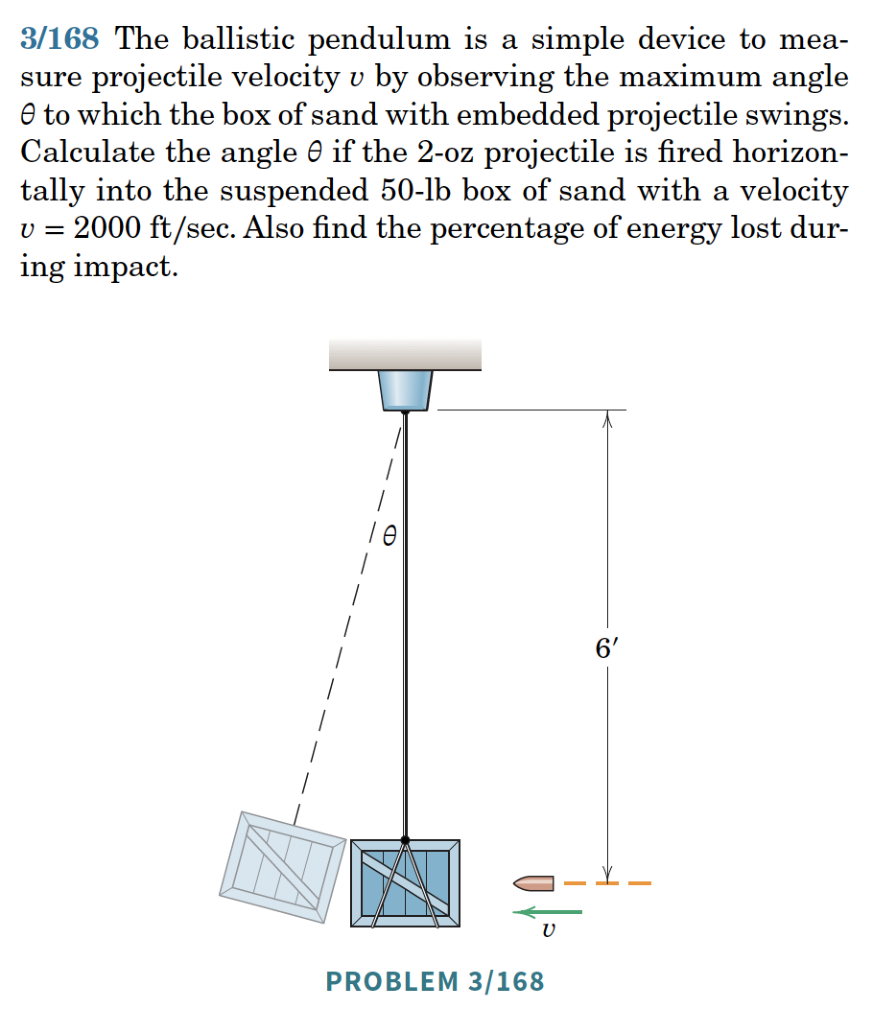
\includegraphics[width=0.5\linewidth,height=\textheight,keepaspectratio]{system_of_particles/../figures/system_of_particles/03-168.png}

}

\caption{MKB 03-168.}

\end{figure}%

\textbf{2.} {[}MKB 03-178{]} Use the integral form of the BoAM; choose
the origin at the green base. \emph{(ans. \(\dot\theta=26.0\) rad/s)}

\begin{figure}[H]

{\centering 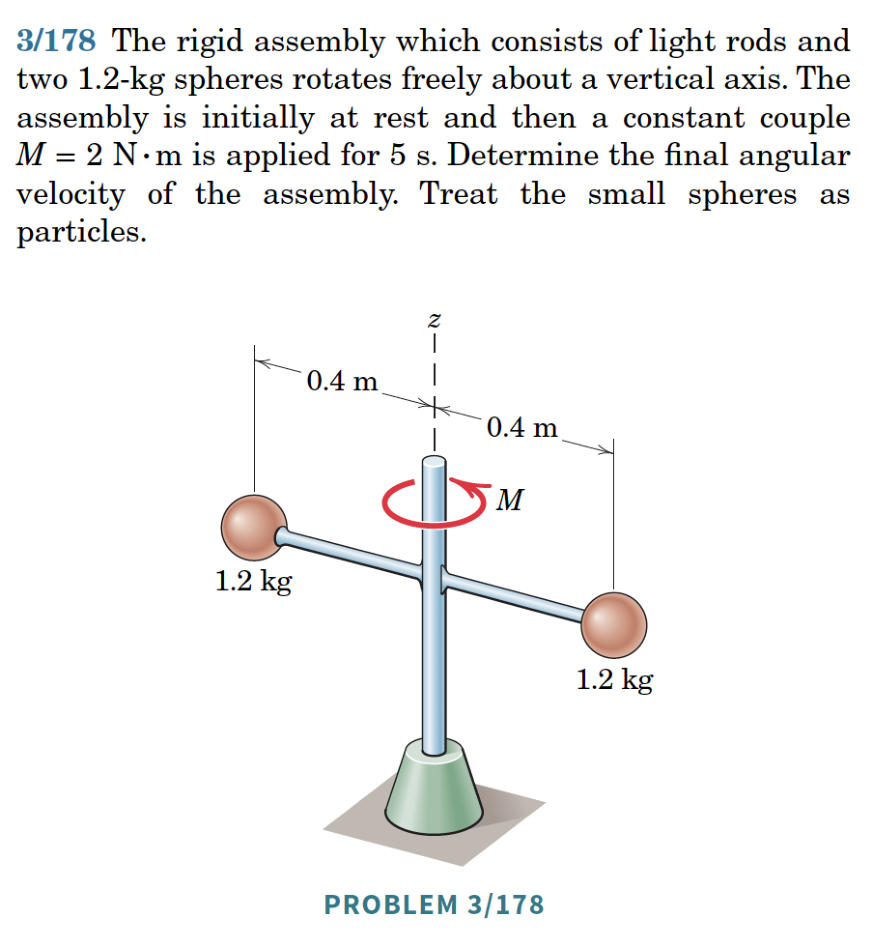
\includegraphics[width=0.5\linewidth,height=\textheight,keepaspectratio]{system_of_particles/../figures/system_of_particles/03-178.png}

}

\caption{MKB 03-178.}

\end{figure}%

\textbf{3.} {[}04-008{]} Take an appropriate cut in the rope.
\emph{(ans. \(T=58.3\) lb)}

\begin{figure}[H]

{\centering 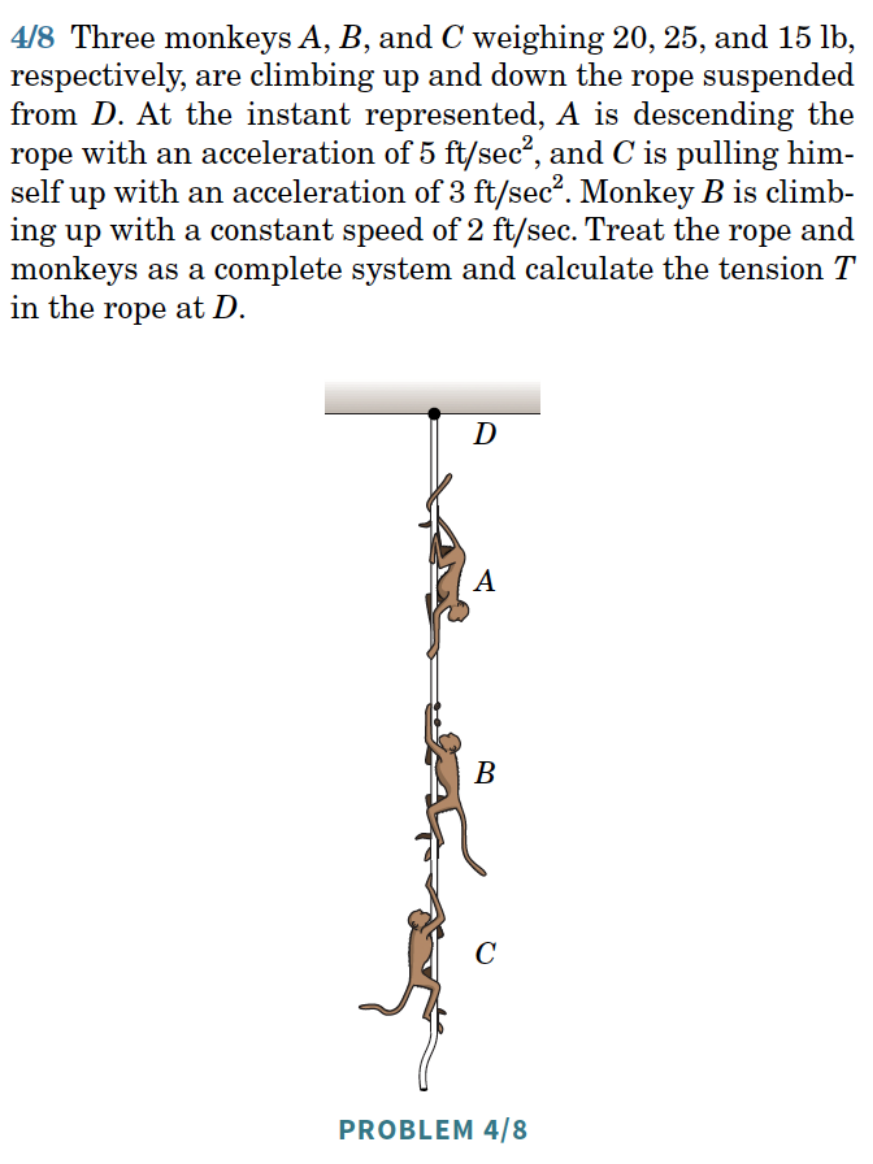
\includegraphics[width=0.5\linewidth,height=\textheight,keepaspectratio]{system_of_particles/../figures/system_of_particles/04-008.png}

}

\caption{MKB 04-008.}

\end{figure}%

\textbf{4.} {[}04-009{]} \emph{(ans. \(D_x=1.288\) lb left, \(D_y=35.5\)
lb up, \(N_E=25.6\) lb up)}

\begin{figure}[H]

{\centering 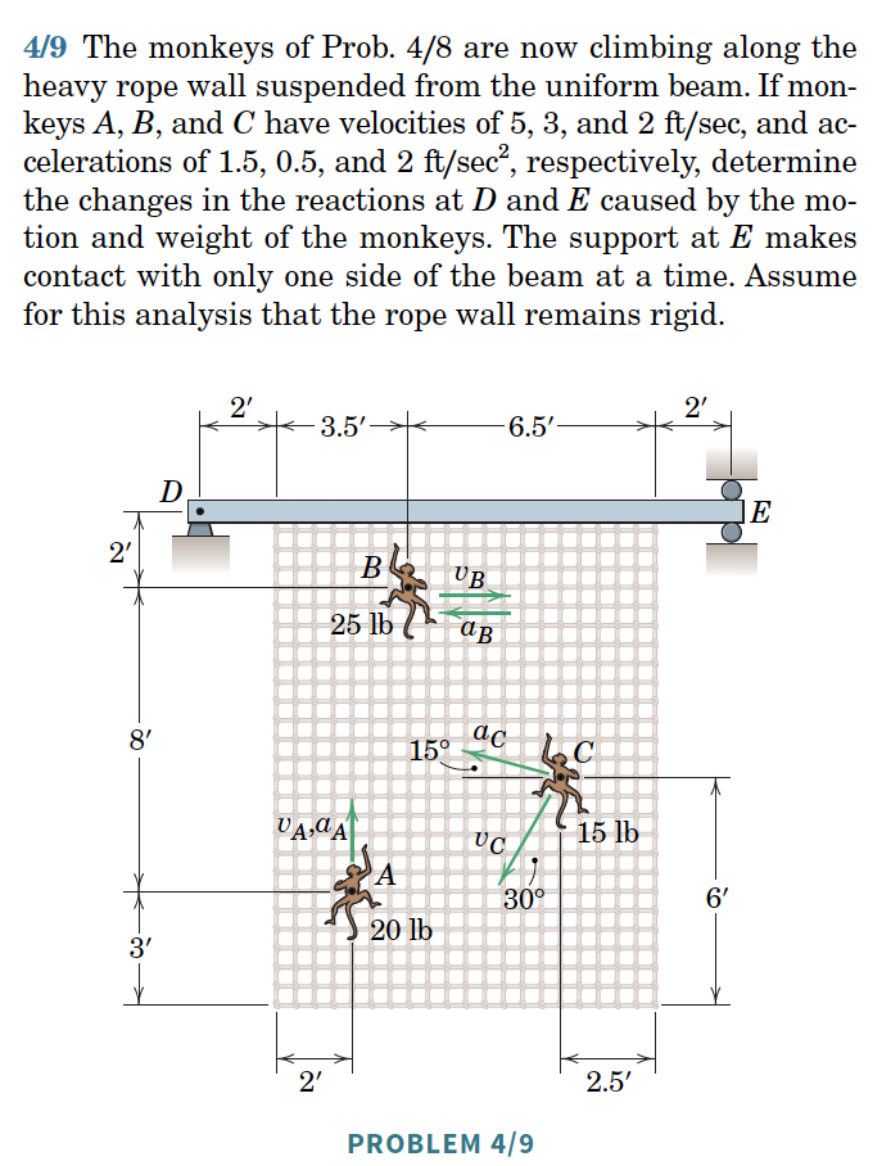
\includegraphics[width=0.5\linewidth,height=\textheight,keepaspectratio]{system_of_particles/../figures/system_of_particles/04-009.png}

}

\caption{MKB 04-009.}

\end{figure}%

\textbf{5.} {[}04-019{]} Identify a direction of linear momentum
conservation; the center of mass remains stationary. \emph{(ans.
\(s=\frac{(m_1+m_2)x_{10}-m_2 l}{m_0+m_1+m_2}\))}

\begin{figure}[H]

{\centering 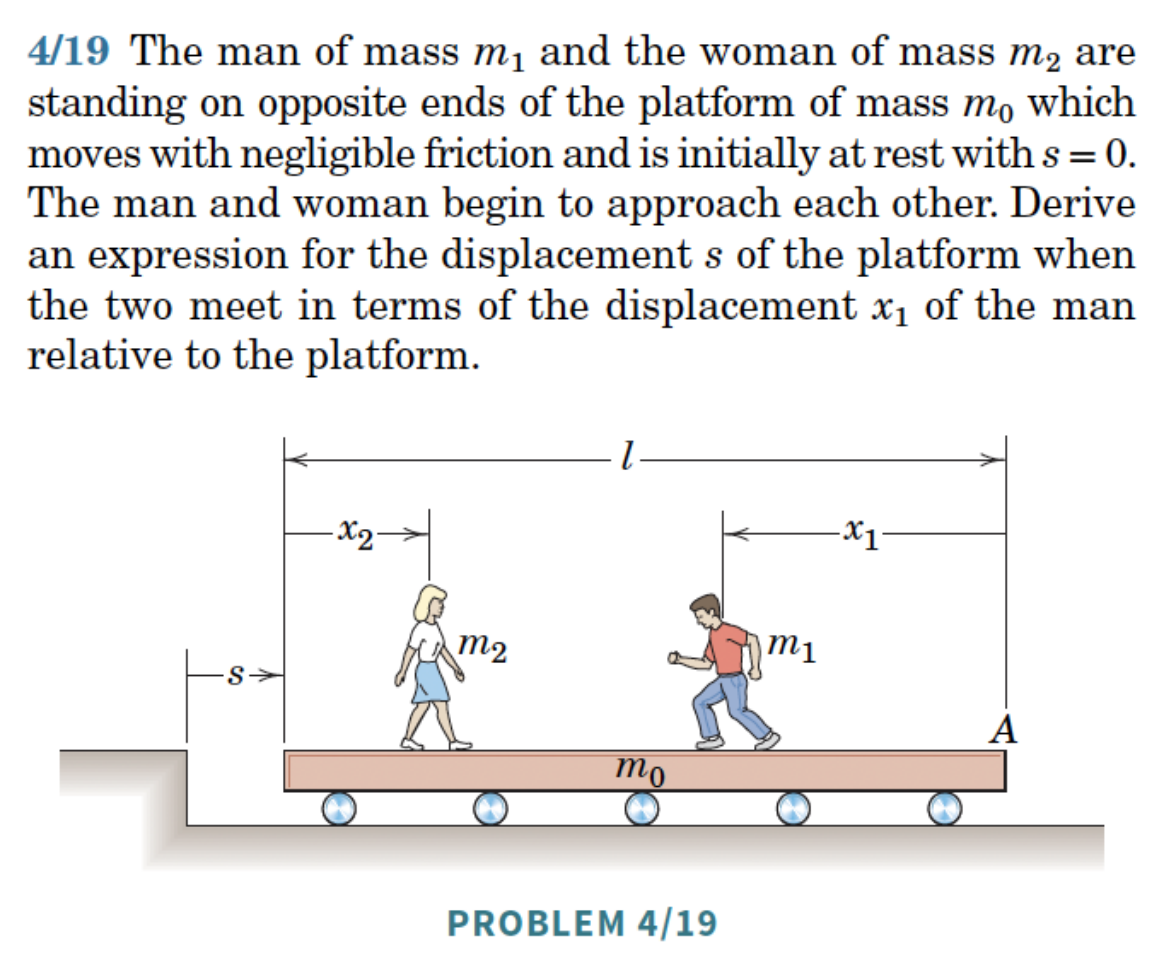
\includegraphics[width=0.5\linewidth,height=\textheight,keepaspectratio]{system_of_particles/../figures/system_of_particles/04-019.png}

}

\caption{MKB 04-019.}

\end{figure}%

\part{Rigid Body Dynamics}

\chapter{Kinematics of Rigid Bodies}\label{kinematics-of-rigid-bodies}

In this chapter, we will denote the fixed basis by
\(\{{\bf E}_1,{\bf E}_2,{\bf E}_3\}\).

Consider a body \(\mathcal{B}\) in motion in 3D space.

\begin{center}
\pandocbounded{
\includegraphics[keepaspectratio]{rigid_body_dynamics/rigid_body_kinematics_files/figure-pdf/unnamed-chunk-1-1.pdf}}
\end{center}

\begin{itemize}
\tightlist
\item
  A body \(\mathcal{B}\) is a collection of material points (mass
  particles or particles).
\item
  It is convenient to define a fixed reference configuration
  \(\boldsymbol{\kappa}_0\) for the body:
  \({\bf X}=\boldsymbol{\kappa}_0\).
\item
  The present (or current) configuration of the body is denoted by
  \(\boldsymbol{\kappa}_t\).
\item
  We denote a material point by \(X\). The position of the material
  point \(X\) relative to a fixed origin at the reference configuration
  is denoted by \({\bf X}\) and at time \(t\) is denoted by \({\bf x}\).
\item
  This motion is invertible; we can use \({\bchi}\) to uniquely define
  the motion as a function of \(X\) and \(t\):
  \({\bf x} = \tilde{\bchi}(X,t) = {\bchi}({\bf X},t)\).
\item
  \(\bchi\) (pronounced like ``kye'') is called the \textbf{motion
  function}. It tells you the current position vector of the material
  point which, at the reference configuration, had position vector
  \({\bf X}\).
\end{itemize}

\begin{tcolorbox}[enhanced jigsaw, arc=.35mm, bottomrule=.15mm, bottomtitle=1mm, breakable, colback=white, colbacktitle=quarto-callout-tip-color!10!white, colframe=quarto-callout-tip-color-frame, coltitle=black, left=2mm, leftrule=.75mm, opacityback=0, opacitybacktitle=0.6, rightrule=.15mm, title=\textcolor{quarto-callout-tip-color}{\faLightbulb}\hspace{0.5em}{Think!}, titlerule=0mm, toprule=.15mm, toptitle=1mm]

\textbf{Question:} What is a mathematical statement that means that a
body is rigid?

\begin{quote}
\textbf{Answer}

For rigid bodies the distance between any two mass particles \(X_1\) and
\(X_2\) remains constant for all motions: \begin{align}
    \lnorm{\bf x}_1-{\bf x}_2\rnorm = \lnorm{\bf X}_1-{\bf X}_2\rnorm.
\end{align} The motion preserves angles between lines on the body
(unlike elastic bodies or fluids) and preserves orientation (it is not a
reflection).
\end{quote}

\end{tcolorbox}

Any rigid body motion can be built in two steps:

\begin{center}
\pandocbounded{
\includegraphics[keepaspectratio]{rigid_body_dynamics/rigid_body_kinematics_files/figure-pdf/unnamed-chunk-2-1.pdf}}
\end{center}

\begin{enumerate}
\def\labelenumi{\arabic{enumi}.}
\tightlist
\item
  \textbf{Rotate} the object about \(O\) until it has the desired
  orientation (but likely the wrong position). This motion maps every
  point \({\bf X}\) to an intermediate position \({\bf x}_I\):
  \({\bf x}_I = {\bf Q}(t){\bf X}\) with
  \(\lnorm{\bf Q}(t){\bf X}\rnorm = \lnorm{\bf X}\rnorm\) for all
  \({\bf X}\).
\item
  \textbf{Translate} via the translation vector \({\bf y}(t)\) (without
  further rotation) from an intermediate configuration to a current
  configuration.
\end{enumerate}

Then every rigid motion is: \begin{align}
    {\bf x} = \bchi({\bf X},t) = {\bf x}_I({\bf X},t)+{\bf y}(t) = {\bf Q}(t){\bf X}+{\bf y}(t).
\end{align} For each rigid motion (and choice of \(O\)), \({\bf Q}(t)\)
and \({\bf y}(t)\) are unique.

\({\bf Q}(t)\) is an object that acts on a vector to produce another
vector. If \({\bf Q}\) is also linear, then we call it a
\textbf{tensor}. We will show that \({\bf Q}(t)\) is a linear map and is
called the \textbf{rotation tensor}. Both \({\bf Q}\) and \({\bf y}\)
are the same for all material points of the rigid body(functions of
\(t\) only) as all material points on the rigid body are rotated and
translated by the same amount.

In this class we consider bodies translating and rotatingin the plane,
ie. \textbf{general plane motion}, where
\(\bomega = \dot{\theta}{\bf E}_3\) and \(\balpha = \dot{\bomega}\). The
fixed axis of rotation is \({\bf E}_3\).

\begin{tcolorbox}[enhanced jigsaw, arc=.35mm, bottomrule=.15mm, bottomtitle=1mm, breakable, colback=white, colbacktitle=quarto-callout-tip-color!10!white, colframe=quarto-callout-tip-color-frame, coltitle=black, left=2mm, leftrule=.75mm, opacityback=0, opacitybacktitle=0.6, rightrule=.15mm, title=\textcolor{quarto-callout-tip-color}{\faLightbulb}\hspace{0.5em}{Think!}, titlerule=0mm, toprule=.15mm, toptitle=1mm]

\textbf{Question:} How do we know if a body has rotated relative to a
reference configuration?

\begin{quote}
\textbf{Answer}

\pandocbounded{
\includegraphics[keepaspectratio]{rigid_body_dynamics/rigid_body_kinematics_files/figure-pdf/unnamed-chunk-3-1.pdf}}

We need the reference configuration to define rotation. The rotation
angle \(\theta\) is the angular displacement of every material line from
reference to current configuration. The axis of rotation is
perpendicular to the page.
\end{quote}

\end{tcolorbox}

\section{Corotational Bases}\label{corotational-bases}

A \emph{corotational basis} \(\{{\bf e}_1,{\bf e}_2\}\) is a pair of
vectors embedded in the material. Initially \({\bf e}_i = {\bf E}_i\).

\begin{center}
\pandocbounded{
\includegraphics[keepaspectratio]{rigid_body_dynamics/rigid_body_kinematics_files/figure-pdf/unnamed-chunk-4-1.pdf}}
\end{center}

For a rigid body, the components of a material vector \({\bf v}\) along
the corotational basis are constant throughout the motion: \begin{align}
    {\bf x} = x_1{\bf e}_1+x_2{\bf e}_2,
\end{align} where \(x_1\) and \(x_2\) are constant and \({\bf e}_1(t)\),
\({\bf e}_2(t)\) evolve with the body. Since initially
\({\bf e}_1 = {\bf E}_1\) and \({\bf e}_2 = {\bf E}_2\), we can write
\({\bf x}(t=0) = x_1{\bf E}_1+x_2{\bf E}_2\).The corotational basis is
unaffected by translation.

\section{Tensors}\label{tensors}

A tensor \({\bf T}\) is a \emph{linear transformation} that transforms a
vector into another vector: \({\bf T}{\bf u} = {\bf v}\). A tensor
exists independent of any basis and is defined by its action on vectors.

Examples:

\begin{itemize}
\item
  A rotation tensor \({\bf Q}\) acting on some vector \({\bf v}\)
  returns a vector \({\bf u}\) that is a rotation of \({\bf v}\) by some
  angle \(\theta\).
\item
  The identity tensor \({\bf I}\) acting on any vector \({\bf v}\)
  returns the same vector \({\bf v}\).
\item
  A scaling tensor \({\bf S}\) acting on some vector \({\bf v}\) returns
  another the scaled vector \(k{\bf v}\).
\end{itemize}

\begin{tcolorbox}[enhanced jigsaw, arc=.35mm, bottomrule=.15mm, bottomtitle=1mm, breakable, colback=white, colbacktitle=quarto-callout-tip-color!10!white, colframe=quarto-callout-tip-color-frame, coltitle=black, left=2mm, leftrule=.75mm, opacityback=0, opacitybacktitle=0.6, rightrule=.15mm, title=\textcolor{quarto-callout-tip-color}{\faLightbulb}\hspace{0.5em}{Think!}, titlerule=0mm, toprule=.15mm, toptitle=1mm]

\textbf{Question:} Is a rotation a linear transformation?

\begin{quote}
\textbf{Answer}

Yes. To be a linear transformation, a rotation would have to satisfy two
rules:

\begin{itemize}
\item
  Rotating \(a{\bf X}\) is the same as rotating \({\bf X}\) and then
  scaling by \(a\).
\item
  Rotating \({\bf X}_1\) and \({\bf X}_2\) is the same as rotating
  \({\bf X}_1\), rotating \({\bf X}_2\), and then adding the results
  together.
\end{itemize}

Since both of these propositions are true for rotations, we conclude
that rotations are linear transformations. Thus, rotations are tensors.
\end{quote}

\end{tcolorbox}

\begin{tcolorbox}[enhanced jigsaw, arc=.35mm, bottomrule=.15mm, bottomtitle=1mm, breakable, colback=white, colbacktitle=quarto-callout-tip-color!10!white, colframe=quarto-callout-tip-color-frame, coltitle=black, left=2mm, leftrule=.75mm, opacityback=0, opacitybacktitle=0.6, rightrule=.15mm, title=\textcolor{quarto-callout-tip-color}{\faLightbulb}\hspace{0.5em}{Think!}, titlerule=0mm, toprule=.15mm, toptitle=1mm]

\textbf{Question:} Are tensors and matrices the same?

\begin{quote}
\textbf{Answer}

We can answer this question using an analogous one: are vectors and
arrays the same?

No.~A vector is an abstract object independent of any basis; an array is
its representation in a specific basis. Similarly, a tensor is not a
matrix, but can be expressed as one in a given coordinate system.

We can represent a vector as an array of numbers if we have chosen a
basis or coordinate system, but a vector is an abstract object that
exists independent of any basis.

Consider for example a position vector \({\bf r}\) to a particle \(P\).
This vector encodes the position of \(P\) relative to the origin
(distance and direction) independent of any basis. We could however
express this vector in the Cartesian basis as
\(x{\bf E}_x+y{\bf E}_y+z{\bf E}_z\). In this basis, we could write the
array \([x,y,z]\) to represent this vector.

Analogously, a tensor is not a matrix, but a tensor can be expressed as
a matrix in a given coordinate system.
\end{quote}

\end{tcolorbox}

\section{Tensor (Bun) Product}\label{tensor-bun-product}

Consider the mathematical object, termed the \textbf{tensor product} of
two vectors: \begin{align}
    {\bf a}\otimes{\bf b},
\end{align} where \({\bf a}\) and \({\bf b}\) are vectors. This object
is defined to act on vectors to produce a vector as follows:
\begin{align}
    \lp {\bf a}\otimes{\bf b} \rp{\bf u} = \lp {\bf b}\cdot{\bf u}\rp{\bf v}.
\end{align} If this object is also linear, then it is a tensor. To
verify that this object is linear, we need to show that \begin{align}
    &\lp {\bf a}\otimes{\bf b}\rp({\bf u}+{\bf v}) = \lp{\bf a}\otimes{\bf b}\rp{\bf u}+\lp{\bf a}\otimes{\bf b}\rp{\bf v},\\
    &\lp {\bf a}\otimes{\bf b}\rp(k{\bf u}) = k(\lp{\bf a}\otimes{\bf b}\rp{\bf u}).
\end{align}

For the first, \begin{align*}
    \lp {\bf a}\otimes{\bf b}\rp({\bf u}+{\bf v}) &= \lp({\bf u}+{\bf v})\cdot{\bf b}\rp{\bf a} 
    = {\bf u}\cdot{\bf b}{\bf a}+{\bf v}\cdot{\bf b}{\bf a}
    = \lp{\bf a}\otimes{\bf b}\rp{\bf u}+\lp{\bf a}\otimes{\bf b}\rp{\bf v}.
\end{align*} For the second, \begin{align}
        \lp{\bf a}\otimes{\bf b}\rp(k{\bf u}) &= (k{\bf u})\cdot{\bf b}{\bf a} = k({\bf u}\cdot{\bf b}{\bf a}) = k(\lp{\bf a}\otimes{\bf b}\rp{\bf u}).
\end{align}

\begin{tcolorbox}[enhanced jigsaw, arc=.35mm, bottomrule=.15mm, bottomtitle=1mm, breakable, colback=white, colbacktitle=quarto-callout-tip-color!10!white, colframe=quarto-callout-tip-color-frame, coltitle=black, left=2mm, leftrule=.75mm, opacityback=0, opacitybacktitle=0.6, rightrule=.15mm, title=\textcolor{quarto-callout-tip-color}{\faLightbulb}\hspace{0.5em}{Think!}, titlerule=0mm, toprule=.15mm, toptitle=1mm]

\textbf{Question:} What does
\(2{\bf E}_1\otimes{\bf E}_1+2{\bf E}_2\otimes{\bf E}_2+2{\bf E}_3\otimes{\bf E}_3\)
do to a vector?

\begin{quote}
\textbf{Answer}

It scales it by a factor of two.
\end{quote}

\end{tcolorbox}

\begin{tcolorbox}[enhanced jigsaw, arc=.35mm, bottomrule=.15mm, bottomtitle=1mm, breakable, colback=white, colbacktitle=quarto-callout-tip-color!10!white, colframe=quarto-callout-tip-color-frame, coltitle=black, left=2mm, leftrule=.75mm, opacityback=0, opacitybacktitle=0.6, rightrule=.15mm, title=\textcolor{quarto-callout-tip-color}{\faLightbulb}\hspace{0.5em}{Think!}, titlerule=0mm, toprule=.15mm, toptitle=1mm]

\textbf{Question:} Show that the identity tensor may be written as
\({\bf E}_1\otimes{\bf E}_1+{\bf E}_2\otimes{\bf E}_2+{\bf E}_3\otimes{\bf E}_3\).

\begin{quote}
\textbf{Answer}

Apply the definition of the tensor product term by term on a vector.
\end{quote}

\end{tcolorbox}

\begin{tcolorbox}[enhanced jigsaw, arc=.35mm, bottomrule=.15mm, bottomtitle=1mm, breakable, colback=white, colbacktitle=quarto-callout-tip-color!10!white, colframe=quarto-callout-tip-color-frame, coltitle=black, left=2mm, leftrule=.75mm, opacityback=0, opacitybacktitle=0.6, rightrule=.15mm, title=\textcolor{quarto-callout-tip-color}{\faLightbulb}\hspace{0.5em}{Think!}, titlerule=0mm, toprule=.15mm, toptitle=1mm]

\textbf{Question:} Show that the rotation tensor \({\bf Q}\) can be
expressed as
\({\bf Q} = {\bf e}_x\otimes{\bf E}_x+{\bf e}_y\otimes{\bf E}_y+{\bf e}_z\otimes{\bf E}_z\).
In other words, show that
\(\lp {\bf e}_x\otimes{\bf E}_x+{\bf e}_y\otimes{\bf E}_y+{\bf e}_z\otimes{\bf E}_z\rp\lp{\bf X}_A-{\bf X}_B\rp = {\bf x}_A-{\bf x}_B\)
where \({\bf X}_A-{\bf X}_B = a{\bf E}_x+b{\bf E}_y\) and
\({\bf x}_A-{\bf x}_B = a{\bf e}_x+b{\bf e}_y\).

\begin{quote}
\textbf{Answer}

\ldots{}
\end{quote}

\end{tcolorbox}

\section{Matrix Representation of
Tensors}\label{matrix-representation-of-tensors}

Given a basis \(\{{\bf e}_1,{\bf e}_2,{\bf e}_3\}\), any tensor
\({\bf Q}\) can be written as a sum of dyads (tensor products) on that
basis: \begin{align}
    {\bf Q} = \sum_{k=1}^3\sum_{\ell=1}^3 Q_{k\ell}\,{\bf e}_k\otimes{\bf e}_\ell.
\end{align} There are two equivalent perspectives for arriving at the
matrix representation of \({\bf Q}\), and both lead to the same
components \(Q_{ij}\).

\subsection{Perspective 1: From the Dyadic
Expansion}\label{perspective-1-from-the-dyadic-expansion}

Acting with \({\bf Q}\) on a basis vector \({\bf e}_j\) and using
\({\bf e}_\ell\cdot{\bf e}_j = 1\) if \(\ell=j\) and \(0\) otherwise:
\begin{align}
    {\bf Q}{\bf e}_j = \lp\sum_{k=1}^3\sum_{\ell=1}^3 Q_{k\ell}\,{\bf e}_k\otimes{\bf e}_\ell\rp{\bf e}_j = \sum_{k=1}^3\sum_{\ell=1}^3 Q_{k\ell}\lp{\bf e}_\ell\cdot{\bf e}_j\rp{\bf e}_k = \sum_{k=1}^3 Q_{kj}\,{\bf e}_k.
\end{align} Taking the dot product with \({\bf e}_i\): \begin{align}
    \lp{\bf Q}{\bf e}_j\rp\cdot{\bf e}_i = \sum_{k=1}^3 Q_{kj}\lp{\bf e}_k\cdot{\bf e}_i\rp = Q_{ij}.
\end{align} So the coefficient \(Q_{ij}\) in the dyadic expansion of
\({\bf Q}\) is exactly the matrix entry in row \(i\), column \(j\).

\subsection{Perspective 2: From the Action on a General
Vector}\label{perspective-2-from-the-action-on-a-general-vector}

Given a basis \(\{{\bf e}_1,{\bf e}_2,{\bf e}_3\}\), every vector
\({\bf X}\) can be written uniquely as
\({\bf X} = X_1{\bf e}_1+X_2{\bf e}_2+X_3{\bf e}_3\) with components
\(X_i = {\bf X}\cdot{\bf e}_i\). By linearity of \({\bf Q}\):
\begin{align}
    {\bf Q}{\bf X} = X_1({\bf Q}{\bf e}_1)+X_2({\bf Q}{\bf e}_2)+X_3({\bf Q}{\bf e}_3).
\end{align} Writing the output vector \({\bf x}\equiv{\bf Q}{\bf X}\) in
the same basis, \({\bf x} = x_1{\bf e}_1+x_2{\bf e}_2+x_3{\bf e}_3\)
with \(x_i = {\bf x}\cdot{\bf e}_i = ({\bf Q}{\bf X})\cdot{\bf e}_i\),
and defining \begin{align}
    Q_{ij} \equiv \lp{\bf Q}{\bf e}_j\rp\cdot{\bf e}_i,
\end{align} we get \begin{align}
    x_1 &= Q_{11}X_1+Q_{12}X_2+Q_{13}X_3,\\
    x_2 &= Q_{21}X_1+Q_{22}X_2+Q_{23}X_3,\\
    x_3 &= Q_{31}X_1+Q_{32}X_2+Q_{33}X_3,
\end{align} which is exactly the matrix equation \begin{align}
    \begin{bmatrix}x_1\\x_2\\x_3\end{bmatrix}
    =
    \begin{bmatrix}Q_{11}&Q_{12}&Q_{13}\\Q_{21}&Q_{22}&Q_{23}\\Q_{31}&Q_{32}&Q_{33}\end{bmatrix}
    \begin{bmatrix}X_1\\X_2\\X_3\end{bmatrix}.
\end{align}

\begin{tcolorbox}[enhanced jigsaw, arc=.35mm, bottomrule=.15mm, bottomtitle=1mm, breakable, colback=white, colbacktitle=quarto-callout-important-color!10!white, colframe=quarto-callout-important-color-frame, coltitle=black, left=2mm, leftrule=.75mm, opacityback=0, opacitybacktitle=0.6, rightrule=.15mm, title=\textcolor{quarto-callout-important-color}{\faExclamation}\hspace{0.5em}{Note!}, titlerule=0mm, toprule=.15mm, toptitle=1mm]

Both perspectives agree on the same definition
\(Q_{ij}=\lp{\bf Q}{\bf e}_j\rp\cdot{\bf e}_i\). Perspective 1
identifies \(Q_{ij}\) as the coefficient of
\({\bf e}_i\otimes{\bf e}_j\) in the dyadic expansion of \({\bf Q}\)
itself; Perspective 2 identifies it as the entry that makes ordinary
matrix-vector multiplication reproduce the action of \({\bf Q}\) on
components. The matrix representation depends on the chosen basis, but
the tensor itself is basis-independent. Transpose, symmetry, and
skew-symmetry of a tensor can be defined without reference to any basis,
but in practice we identify them through the matrix representation:
\({\bf T}\) is symmetric if \([{\bf T}]=[{\bf T}]^T\) and skew if
\([{\bf T}]=-[{\bf T}]^T\).

\end{tcolorbox}

\subsection{Rigid Body Motion}\label{rigid-body-motion}

In matrix form, rigid body motion is: \begin{align}
    \begin{bmatrix}x_1\\x_2\\x_3\end{bmatrix}
    =
    \begin{bmatrix}Q_{11}(t)&Q_{12}(t)&Q_{13}(t)\\Q_{21}(t)&Q_{22}(t)&Q_{23}(t)\\Q_{31}(t)&Q_{32}(t)&Q_{33}(t)\end{bmatrix}
    \begin{bmatrix}X_1\\X_2\\X_3\end{bmatrix}
    +
    \begin{bmatrix}y_1\\y_2\\y_3\end{bmatrix}.
\end{align} For \([{\bf Q}(t)]\) to be a rotation matrix:
\({\bf Q}{\bf Q}^T = {\bf I}\) and \(\det([{\bf Q}]) = 1\).

\begin{tcolorbox}[enhanced jigsaw, arc=.35mm, bottomrule=.15mm, bottomtitle=1mm, breakable, colback=white, colbacktitle=quarto-callout-tip-color!10!white, colframe=quarto-callout-tip-color-frame, coltitle=black, left=2mm, leftrule=.75mm, opacityback=0, opacitybacktitle=0.6, rightrule=.15mm, title=\textcolor{quarto-callout-tip-color}{\faLightbulb}\hspace{0.5em}{Think!}, titlerule=0mm, toprule=.15mm, toptitle=1mm]

\textbf{Question:} Verify that the matrix representation of the rotation
tensor \({\bf Q}\) of a rotation about \({\bf E}_z\) is \begin{align*}
    \mathtt{Q} = \begin{bmatrix}\cos\theta & -\sin\theta & 0\\\sin\theta & \cos\theta & 0\\0 & 0 & 1\end{bmatrix}
\end{align*} where \(\theta\) is a function of \(t\). Recall that the
rotation tensor can be expressed as \begin{align*}
    {\bf Q} = {\bf e}_1\otimes{\bf E}_1+{\bf e}_2\otimes{\bf E}_2+{\bf e}_3\otimes{\bf E}_3,
\end{align*} and for a rotation about \({\bf E}_3\), we have
\begin{align*}
    {\bf e}_1 &= \cos(\theta){\bf E}_1+\sin(\theta){\bf E}_2,\\
    {\bf e}_2 &= -\sin(\theta){\bf E}_1+\cos(\theta){\bf E}_2.
\end{align*}

\begin{quote}
\textbf{Answer}

Compute
\(Q_{ij} = \lp{\bf Q}{\bf E}_j\rp\cdot{\bf E}_i = {\bf e}_j\cdot{\bf E}_i\)
to recover the matrix.
\end{quote}

\end{tcolorbox}

\begin{tcolorbox}[enhanced jigsaw, arc=.35mm, bottomrule=.15mm, bottomtitle=1mm, breakable, colback=white, colbacktitle=quarto-callout-tip-color!10!white, colframe=quarto-callout-tip-color-frame, coltitle=black, left=2mm, leftrule=.75mm, opacityback=0, opacitybacktitle=0.6, rightrule=.15mm, title=\textcolor{quarto-callout-tip-color}{\faLightbulb}\hspace{0.5em}{Think!}, titlerule=0mm, toprule=.15mm, toptitle=1mm]

\textbf{Question:} A tensor has the following matrix representation on
\(\{{\bf E}_1,{\bf E}_2,{\bf E}_3\}\). What does this rotation matrix do
to a vector?

\begin{align*}
    \mathtt{Q} = 
    \begin{bmatrix}
        \cos(\theta) & -\sin(\theta) & 0\\
        \sin(\theta) & \cos(\theta) & 0\\
        0 & 0 & 1
    \end{bmatrix}
\end{align*}

\begin{quote}
\textbf{Answer}

It rotates vector anti-clockwise by \(\theta = t\) in the \(xy-\)plane.

Check this a few examples: \begin{align*}
    \begin{bmatrix}
        \cos(t) & -\sin(t) & 0\\
        \sin(t) & \cos(t) & 0\\
        0 & 0 & 1
    \end{bmatrix}
    \begin{bmatrix}
        1\\
        0\\
        0
    \end{bmatrix}
    =
    \begin{bmatrix}
        \cos(t)\\
        \sin(t)\\
        0
    \end{bmatrix}
\end{align*} \begin{align*}
    \begin{bmatrix}
        \cos(t) & -\sin(t) & 0\\
        \sin(t) & \cos(t) & 0\\
        0 & 0 & 1
    \end{bmatrix}
    \begin{bmatrix}
        0\\
        1\\
        0
    \end{bmatrix}
    =
    \begin{bmatrix}
        -\sin(t)\\
        \cos(t)\\
        0
    \end{bmatrix}
\end{align*} \begin{align*}
    \begin{bmatrix}
        \cos(t) & -\sin(t) & 0\\
        \sin(t) & \cos(t) & 0\\
        0 & 0 & 1
    \end{bmatrix}
    \begin{bmatrix}
        0\\
        0\\
        1
    \end{bmatrix}
    =
    \begin{bmatrix}
        0\\
        0\\
        1
    \end{bmatrix}
\end{align*} In general, this matrix is a rotation matrix that rotates
vectors \(\theta(t)\) radians anti-clockwise about \({\bf e}_z\).
\end{quote}

\end{tcolorbox}

\begin{tcolorbox}[enhanced jigsaw, arc=.35mm, bottomrule=.15mm, bottomtitle=1mm, breakable, colback=white, colbacktitle=quarto-callout-important-color!10!white, colframe=quarto-callout-important-color-frame, coltitle=black, left=2mm, leftrule=.75mm, opacityback=0, opacitybacktitle=0.6, rightrule=.15mm, title=\textcolor{quarto-callout-important-color}{\faExclamation}\hspace{0.5em}{Note!}, titlerule=0mm, toprule=.15mm, toptitle=1mm]

This matrix satisfies \(\mathtt{Q}\mathtt{Q}^T = \mathtt{I}\) and
\(\det(\mathtt{Q})=1\), so \({\bf Q}\) is a \textbf{proper orthogonal
tensor}. It can be shown that all proper orthogonal tensors are
rotations and vice versa.

\end{tcolorbox}

\section{The Angular Velocity Vector}\label{the-angular-velocity-vector}

From rigid body motion, for any two material points \(A\) and \(B\):
\begin{align}
    {\bf x}_A &= {\bf Q}{\bf X}_A+{\bf q},\\
    {\bf x}_B &= {\bf Q}{\bf X}_B+{\bf q}.
\end{align} Thus,
\(({\bf x}_B-{\bf x}_A) = {\bf Q}({\bf X}_B-{\bf X}_A)\), where
\({\bf Q}\) is a proper orthogonal tensor, meaning that
\({\bf Q}{\bf Q}^T = {\bf I}\) and \(\det({\bf Q}) = 1\).
Differentiating: \begin{align}
    {\bf v}_B-{\bf v}_A =\dot{\bf Q}({\bf X}_B-{\bf X}_A) = \dot{\bf Q}{\bf Q}^T({\bf x}_B-{\bf x}_A).
\end{align} The taking the derivative of \({\bf Q}{\bf Q}^T={\bf I}\),
we show that \(\dot{\bf Q}{\bf Q}^T\) is a skew tensor. \begin{align}
    & \frac{d}{dt}({\bf Q}{\bf Q}^T) = {\bf 0} = \dot{\bf Q}{\bf Q}^T+{\bf Q}\dot{\bf Q}^T,\\
    & \dot{\bf Q}{\bf Q}^T = -{\bf Q}\dot{\bf Q}^T = -(\dot{\bf Q}{\bf Q}^T)^T.
\end{align}

\begin{tcolorbox}[enhanced jigsaw, arc=.35mm, bottomrule=.15mm, bottomtitle=1mm, breakable, colback=white, colbacktitle=quarto-callout-important-color!10!white, colframe=quarto-callout-important-color-frame, coltitle=black, left=2mm, leftrule=.75mm, opacityback=0, opacitybacktitle=0.6, rightrule=.15mm, title=\textcolor{quarto-callout-important-color}{\faExclamation}\hspace{0.5em}{Note!}, titlerule=0mm, toprule=.15mm, toptitle=1mm]

Every skew tensor corresponds to a vector cross product. In the
Cartesian basis, if \({\bf a} = a_1{\bf E}_1+a_2{\bf E}_2+a_3{\bf E}_3\)
and \({\bf b} = b_1{\bf E}_1+b_2{\bf E}_2+b_3{\bf E}_3\), then
\begin{align}
    {\bf a}\times{\bf b} = (a_2b_3-a_3b_2){\bf E}_1-(a_1b_3-a_3){\bf E}_2+(a_1b_2-a_2b_1){\bf E}_3,
\end{align} which can be re-written in matrix form (using the Cartesian
basis) as \begin{align}
    [{\bf a}\times{\bf b}] = \underbrace{\begin{bmatrix}0&-a_3&a_2\\a_3&0&-a_1\\-a_2&a_1&0\end{bmatrix}}_{[{\bf a}]_\times}\begin{bmatrix}b_1\\b_2\\b_3\end{bmatrix}.
\end{align} The skew matrix \([{\bf a}]_\times\) built from the
components of \({\bf a}\) is the matrix representation of the skew
tensor whose axial vector is \({\bf a}\). Applying this to
\(\dot{\bf Q}{\bf Q}^T\) identifies its axial vector as \(\bomega\), so:

\end{tcolorbox}

\begin{align}
    {\bf v}_B-{\bf v}_A = \bomega\times({\bf x}_B-{\bf x}_A).
\end{align} The tensor \(\bOmega = \dot{\bf Q}{\bf Q}^T\) is the
\textbf{angular velocity tensor} and \(\bomega\) is the \textbf{angular
velocity vector}. Taking another derivative: \begin{align}
    {\bf a}_B-{\bf a}_A = \balpha\times({\bf x}_B-{\bf x}_A)+\bomega\times(\bomega\times({\bf x}_B-{\bf x}_A))
\end{align} where \(\balpha\) is the angular acceleration.

\begin{tcolorbox}[enhanced jigsaw, arc=.35mm, bottomrule=.15mm, bottomtitle=1mm, breakable, colback=white, colbacktitle=quarto-callout-important-color!10!white, colframe=quarto-callout-important-color-frame, coltitle=black, left=2mm, leftrule=.75mm, opacityback=0, opacitybacktitle=0.6, rightrule=.15mm, title=\textcolor{quarto-callout-important-color}{\faExclamation}\hspace{0.5em}{Note!}, titlerule=0mm, toprule=.15mm, toptitle=1mm]

For any corotational basis vector \({\bf e}_i\) fixed to the rigid body:
\begin{align}
    \dot{\bf e}_i = \bomega\times{\bf e}_i, \quad i=1,2,3.
\end{align}

\end{tcolorbox}

\section{Velocity and Acceleration of Two Material
Points}\label{velocity-and-acceleration-of-two-material-points}

Let \(A\) and \(B\) be material points on the rigid body. Expressing
\({\bf x}_{B/A}\) on a corotational basis (constant components):
\begin{align}
    {\bf x}_{B/A} &= x{\bf e}_x+y{\bf e}_y,\\
    {\bf v}_{B/A} &= x\dot{\bf e}_x+y\dot{\bf e}_y = \bomega\times{\bf x}_{B/A},\\
    {\bf a}_{B/A} &= \balpha\times{\bf x}_{B/A}+\bomega\times(\bomega\times{\bf x}_{B/A}).
\end{align} Here, \(\bomega = \omega{\bf E}_z\) and
\(\balpha = \alpha{\bf E}_z\) are the previously defined angular
velocity and angular acceleration of the rigid body (in general,
\(\bomega\) and \(\balpha\) are not necessarily constrained to be along
\({\bf E}_3\)). With \(\bomega = \omega{\bf E}_z\) and
\(\balpha = \alpha{\bf E}_z\): \begin{align}
    \omega\,d\omega = \alpha\,d\theta, \qquad \omega\,dt = d\theta, \qquad \alpha\,dt = d\omega.
\end{align}

\begin{tcolorbox}[enhanced jigsaw, arc=.35mm, bottomrule=.15mm, bottomtitle=1mm, breakable, colback=white, colbacktitle=quarto-callout-important-color!10!white, colframe=quarto-callout-important-color-frame, coltitle=black, left=2mm, leftrule=.75mm, opacityback=0, opacitybacktitle=0.6, rightrule=.15mm, title=\textcolor{quarto-callout-important-color}{\faExclamation}\hspace{0.5em}{Note!}, titlerule=0mm, toprule=.15mm, toptitle=1mm]

\begin{itemize}
\tightlist
\item
  \({\bf v}_{B/A} = \bomega\times{\bf x}_{B/A}\) is an expression of
  rigidity: \(\frac{d}{dt}({\bf x}_{B/A})={\bf 0}\).
\item
  The angular velocity and angular acceleration are properties of the
  rigid body. All material lines on the rigid body rotate with the same
  angular velocity and angular acceleration.
\end{itemize}

\end{tcolorbox}

\section{Particle in a Noninertial
Frame}\label{particle-in-a-noninertial-frame}

A noninertial frame is one that accelerates (e.g.~an accelerating bus, a
merry-go-round).

Consider two points: \(A\) is a material point of a rigid body and \(B\)
moves relative to it, then \begin{align}
    {\bf x}_B-{\bf x}_A &= x{\bf e}_x+y{\bf e}_y,\\
    {\bf v}_B-{\bf v}_A &= \bomega\times({\bf x}_B-{\bf x}_A)+\overset{\circ}{\bf x}_{B/A},\\
    {\bf a}_B-{\bf a}_A &= \balpha\times({\bf x}_B-{\bf x}_A)+\bomega\times\lp\bomega\times\lp{\bf x}_B-{\bf x}_A\rp\rp+2\bomega\times\overset{\circ}{\bf x}_{B/A}+\overset{\circ\circ}{\bf x}_{B/A},
\end{align} where
\(\overset{\circ}{\bf x}_{B/A} = \dot{x}{\bf e}_x+\dot{y}{\bf e}_y\) and
\(\overset{\circ\circ}{\bf x}_{B/A} = \ddot{x}{\bf e}_x+\ddot{y}{\bf e}_y\)
are the first and second \textbf{corotational rates}. These are the
velocity and acceleration of \(B\) with respect to \(A\) as observed
from the noninertial frame (ie. an observer fixed to the rigid body).
The term \(2\bomega\times\overset{\circ}{\bf x}_{B/A}\) is the
\textbf{Coriolis acceleration} and
\(\bomega\times(\bomega\times{\bf x}_{B/A})\) is the \textbf{centripetal
acceleration}.

\begin{tcolorbox}[enhanced jigsaw, arc=.35mm, bottomrule=.15mm, bottomtitle=1mm, breakable, colback=white, colbacktitle=quarto-callout-important-color!10!white, colframe=quarto-callout-important-color-frame, coltitle=black, left=2mm, leftrule=.75mm, opacityback=0, opacitybacktitle=0.6, rightrule=.15mm, title=\textcolor{quarto-callout-important-color}{\faExclamation}\hspace{0.5em}{Note!}, titlerule=0mm, toprule=.15mm, toptitle=1mm]

Consider a particle \(B\) whose motion is described by a noninertial
frame with origin \(A\), angular velocity \(\bomega\) and angular
acceleration \(\balpha\). In an inertial frame, the balance of linear
momentum for particle \(B\) applies: \begin{align}
    {\bf F} &= m{\bf a}_B,\\
    {\bf F} &= m\left({\bf a}_A+\balpha\times({\bf x}_B-{\bf x}_A)+\bomega\times\lp\bomega\times\lp{\bf x}_B-{\bf x}_A\rp\rp+2\bomega\times\overset{\circ}{\bf x}_{B/A}+\overset{\circ\circ}{\bf x}_{B/A}\right),\\
    {\bf F}-m\left({\bf a}_A+\balpha\times({\bf x}_B-{\bf x}_A)+\bomega\times\lp\bomega\times\lp{\bf x}_B-{\bf x}_A\rp\rp+2\bomega\times\overset{\circ}{\bf x}_{B/A}\right) &= m\overset{\circ\circ}{\bf x}_{B/A}
\end{align}. The balance of linear momentum for particle \(B\) in the
noninertial frame is the same as in an inertial frame, except that the
fictitious forces
\(-m\left({\bf a}_A+\balpha\times({\bf x}_B-{\bf x}_A)+\bomega\times\lp\bomega\times\lp{\bf x}_B-{\bf x}_A\rp\rp+2\bomega\times\overset{\circ}{\bf x}_{B/A}\right)\)
must be included.

\end{tcolorbox}

\subsection{Merry-go-round}\label{merry-go-round}

\begin{tcolorbox}[enhanced jigsaw, arc=.35mm, bottomrule=.15mm, bottomtitle=1mm, breakable, colback=white, colbacktitle=quarto-callout-tip-color!10!white, colframe=quarto-callout-tip-color-frame, coltitle=black, left=2mm, leftrule=.75mm, opacityback=0, opacitybacktitle=0.6, rightrule=.15mm, title=\textcolor{quarto-callout-tip-color}{\faLightbulb}\hspace{0.5em}{Think!}, titlerule=0mm, toprule=.15mm, toptitle=1mm]

\textbf{Question:} Watch the below video of people playing catch on a
merry-go-round. A ball is thrown on a merry-go-round rotating about
fixed center \(O\), with \({\bf r}_0 = -R{\bf E}_x\) and
\({\bf v}_0 = v_0{\bf E}_x\). The merry-go-round has an angular velocity
\(\bomega\) and an angular acceleration \(\balpha\). What are the
velocity and acceleration of the ball that is appears to have with
respect to an observer on the merry-go-round?

\url{https://www.youtube.com/watch?v=mPsLanVS1Q8}

\begin{quote}
\textbf{Answer}

The ball \(P\) is a projectile so its absolute acceleration, velocity
and position vectors are respectively \begin{align}
    {\bf a} &= -g{\bf E}_z,\\
    {\bf v} &= -gt{\bf E}_z+{\bf v}_0,\\
    {\bf r} &= -\frac{g}{2}t^2+{\bf v}_0t+{\bf r}_0.
\end{align} Conducting a velocity analysis between the ball and the
origin \(O\), we get \begin{align}
    {\bf v} = \bomega\times({\bf r}-{\bf r}_0)+\overset{\circ}{\bf x}_{P/O}.
\end{align} The relative velocity being the only unknown in this
equation, we can solve for it: \begin{align}
    \overset{\circ}{\bf x}_{P/O} = -gt{\bf E}_z+v_0{\bf E}_x+\omega(v_0t{\bf E}_y-R{\bf E}_y).
\end{align}
\end{quote}

\end{tcolorbox}

Another example of this observed in the Foucault pendulum, where the
plane of oscillation of the pendulum appears to rotate with respect to
the Earth. The Coriolis effect is responsible for this apparent
rotation.

\url{https://www.youtube.com/shorts/kbHYp3H3mDE}

\section{Classifications of Rigid Body
Motions}\label{classifications-of-rigid-body-motions}

\textbf{Pure (rectilinear) translation:} \(\bomega = {\bf 0}\),
\(\balpha = {\bf 0}\).

\textbf{Curvilinear translation:} material points follow parallel curved
paths; \(\bomega = {\bf 0}\), \(\balpha = {\bf 0}\)
(e.g.~\href{https://www.youtube.com/watch?v=LU_xVr4b2qM&t=387s}{Ferris
wheel bucket}).

\textbf{Fixed point rotation:} \(\bomega \neq {\bf 0}\), fixed point
with \({\bf v}_O = {\bf a}_O = {\bf 0}\) (e.g.~pendulum): \begin{align}
    {\bf a}_P = \balpha\times{\bf r}_P+\bomega\times(\bomega\times{\bf r}_P).
\end{align} The term \(\balpha\times{\bf r}_P\) is the tangential
acceleration; \(\bomega\times(\bomega\times{\bf r}_P)\) is the
centripetal acceleration.

\textbf{General motion:} combined translation and rotation.

\section{Instantaneous Center of
Rotation}\label{instantaneous-center-of-rotation}

\begin{tcolorbox}[enhanced jigsaw, arc=.35mm, bottomrule=.15mm, bottomtitle=1mm, breakable, colback=white, colbacktitle=quarto-callout-tip-color!10!white, colframe=quarto-callout-tip-color-frame, coltitle=black, left=2mm, leftrule=.75mm, opacityback=0, opacitybacktitle=0.6, rightrule=.15mm, title=\textcolor{quarto-callout-tip-color}{\faLightbulb}\hspace{0.5em}{Think!}, titlerule=0mm, toprule=.15mm, toptitle=1mm]

\textbf{Question:} Draw the velocity profile of a rotating link with a
fixed end.

\begin{quote}
\textbf{Answer}

\pandocbounded{
\includegraphics[keepaspectratio]{rigid_body_dynamics/rigid_body_kinematics_files/figure-pdf/unnamed-chunk-5-1.pdf}}
\end{quote}

\end{tcolorbox}

For a body in fixed point rotation, the velocity of each point on the
body is perpendicular to the position vector from the axis of rotation
to this point.

\begin{tcolorbox}[enhanced jigsaw, arc=.35mm, bottomrule=.15mm, bottomtitle=1mm, breakable, colback=white, colbacktitle=quarto-callout-tip-color!10!white, colframe=quarto-callout-tip-color-frame, coltitle=black, left=2mm, leftrule=.75mm, opacityback=0, opacitybacktitle=0.6, rightrule=.15mm, title=\textcolor{quarto-callout-tip-color}{\faLightbulb}\hspace{0.5em}{Think!}, titlerule=0mm, toprule=.15mm, toptitle=1mm]

\textbf{Question:} Draw the velocity profile of a sphere rotating about
its fixed center, or of a random rigid body in fixed point rotation.

\begin{quote}
\textbf{Answer}

\ldots{}
\end{quote}

\end{tcolorbox}

A body in general plane motion is not rotating about a fixed point, but
\textbf{instantaneously} it rotates about the \textbf{instantaneous
center of rotation (IC)} --- a point with zero velocity at that instant.
If \({\bf v}_{IC} = {\bf 0}\), then for any material point \(A\):
\begin{align}
    {\bf v}_A = \bomega\times({\bf r}_A-{\bf r}_{IC}).
\end{align} So \({\bf r}_{A/IC}\) is perpendicular to \({\bf v}_A\).
Knowing the directions of \({\bf v}_A\) and \({\bf v}_B\) for two
material points identifies the IC.

\begin{center}
\pandocbounded{
\includegraphics[keepaspectratio]{rigid_body_dynamics/rigid_body_kinematics_files/figure-pdf/unnamed-chunk-6-1.pdf}}
\end{center}

For the IC at this instant: \begin{align}
    \begin{split}
        {\bf v}_P &= \bomega\times{\bf r}_{P/IC},\\
        {\bf a}_P &= \balpha\times{\bf r}_{P/IC}+\bomega\times(\bomega\times{\bf r}_{P/IC}).
    \end{split}
\end{align}

\begin{tcolorbox}[enhanced jigsaw, arc=.35mm, bottomrule=.15mm, bottomtitle=1mm, breakable, colback=white, colbacktitle=quarto-callout-important-color!10!white, colframe=quarto-callout-important-color-frame, coltitle=black, left=2mm, leftrule=.75mm, opacityback=0, opacitybacktitle=0.6, rightrule=.15mm, title=\textcolor{quarto-callout-important-color}{\faExclamation}\hspace{0.5em}{Note!}, titlerule=0mm, toprule=.15mm, toptitle=1mm]

\begin{itemize}
\item
  The IC of a RB does not have to be on the RB itself, however, the IC
  behaves like a material point of the RB. One could consider a massless
  extension of the RB which containts the IC.
\item
  The IC can only be used for velocity analysis since its acceleration
  is nonzero.
\item
  The IC generally migrates through space.
\item
  For a translating rigid body the IC is at infinity.
\end{itemize}

\end{tcolorbox}

\textbf{Procedure:}

\begin{itemize}
\tightlist
\item
  Use geometry to find the IC.
\item
  Find \(|\omega| = \lnorm\bomega\rnorm\) using
  \({\bf v}_P=\bomega\times{\bf r}_{P/IC}\).
\item
  Get \({\bf v}_P\) for any point \(P\).
\end{itemize}

\emph{Examples: Rod falling on corner and
\href{https://www.youtube.com/watch?v=RDixpdSGERQ}{Crank slider}.}

\url{https://youtu.be/E_5JPTllkDU}

\section{Doing Kinematics
Geometrically}\label{doing-kinematics-geometrically}

In some problems, we can use the laws of geometry that are true for
every time and are differentiable.

\emph{Example: Problem 5/31.}

Focus on triangle \(OAB\):

\begin{itemize}
\item
  Let \(\alpha\) be the angle \(OAB\).
\item
  Let \(\beta\) be the angle \(BOA\). \(\dot{\beta}\) is the angular
  velocity of bar \(OA\).
\item
  Let \(\theta\) be the angle \(OBA\). \(\dot{\theta}\) is the angular
  velocity of bar \(BC\).
\item
  The law of sines holds at all times.
\item
  The law of cosines holds at all times.
\item
  The fact that \(OAB\) is a triangle holds at all times, so
  \(\beta+\alpha+\theta=\pi\), which we can differentiate.
\end{itemize}

\section{Kinematics of Rolling and
Sliding}\label{kinematics-of-rolling-and-sliding}

\begin{tcolorbox}[enhanced jigsaw, arc=.35mm, bottomrule=.15mm, bottomtitle=1mm, breakable, colback=white, colbacktitle=quarto-callout-important-color!10!white, colframe=quarto-callout-important-color-frame, coltitle=black, left=2mm, leftrule=.75mm, opacityback=0, opacitybacktitle=0.6, rightrule=.15mm, title=\textcolor{quarto-callout-important-color}{\faExclamation}\hspace{0.5em}{Note!}, titlerule=0mm, toprule=.15mm, toptitle=1mm]

Terminology: ``rolling'' = roll without slip; ``sliding'' = roll with
slip.

\end{tcolorbox}

Consider a rigid body \(\mathcal{B}\) in contact with a fixed surface
\(\mathcal{S}\). Let \(P\) be the material point of \(\mathcal{B}\) in
contact at time \(t\), with unit normal \({\bf n}\) to \(\mathcal{S}\).

Since \(P\) belongs to \(\mathcal{B}\): \begin{align}
    {\bf v}_P-{\bf v}_C &= \bomega\times({\bf r}_P-{\bf r}_C),\\
    {\bf a}_P-{\bf a}_C &= \balpha\times({\bf r}_P-{\bf r}_C)+\bomega\times\lp\bomega\times({\bf r}_P-{\bf r}_C)\rp.
\end{align}

\begin{itemize}
\tightlist
\item
  \textbf{Contact (touching):} \({\bf v}_P\cdot{\bf n} = 0\). Thus,
  \({\bf v}_C\cdot{\bf n} = -\bomega\times({\bf r}_P-{\bf r}_C)\cdot{\bf n}\).
\item
  \textbf{Rolling (no slip):} \({\bf v}_P = {\bf 0}\), so
  \({\bf v}_C = -\bomega\times({\bf r}_P-{\bf r}_C)\). Note:
  \({\bf a}_P \neq {\bf 0}\) in general.
\end{itemize}

\subsection{Example: Rolling Circular
Disk}\label{example-rolling-circular-disk}

\begin{tcolorbox}[enhanced jigsaw, arc=.35mm, bottomrule=.15mm, bottomtitle=1mm, breakable, colback=white, colbacktitle=quarto-callout-tip-color!10!white, colframe=quarto-callout-tip-color-frame, coltitle=black, left=2mm, leftrule=.75mm, opacityback=0, opacitybacktitle=0.6, rightrule=.15mm, title=\textcolor{quarto-callout-tip-color}{\faLightbulb}\hspace{0.5em}{Think!}, titlerule=0mm, toprule=.15mm, toptitle=1mm]

\textbf{Question:} What is the IC of a rolling disk?

\begin{quote}
\textbf{Answer}

The contact point with the surface.
\end{quote}

\end{tcolorbox}

\begin{tcolorbox}[enhanced jigsaw, arc=.35mm, bottomrule=.15mm, bottomtitle=1mm, breakable, colback=white, colbacktitle=quarto-callout-tip-color!10!white, colframe=quarto-callout-tip-color-frame, coltitle=black, left=2mm, leftrule=.75mm, opacityback=0, opacitybacktitle=0.6, rightrule=.15mm, title=\textcolor{quarto-callout-tip-color}{\faLightbulb}\hspace{0.5em}{Think!}, titlerule=0mm, toprule=.15mm, toptitle=1mm]

\textbf{Question:} Draw the velocity profile of a wheel that is rolling
without slipping on a road.

\begin{quote}
\textbf{Answer}

\ldots{}
\end{quote}

\end{tcolorbox}

\begin{center}
\pandocbounded{
\includegraphics[keepaspectratio]{rigid_body_dynamics/rigid_body_kinematics_files/figure-pdf/unnamed-chunk-7-1.pdf}}
\end{center}

Consider an upright homogeneous disk of radius \(R\) rolling on a plane,
with angular velocity \(\bomega=\omega{\bf E}_z\) and angular
acceleration \(\balpha=\alpha{\bf E}_z\). The center of mass \(C\) moves
in rectilinear motion: \begin{align}
    {\bf r}_C = x{\bf E}_x+c{\bf E}_y, \qquad {\bf v}_C = \dot{x}{\bf E}_x, \qquad {\bf a}_C = \ddot{x}{\bf E}_x.
\end{align} Define a corotational basis for the disk: \begin{align}
    {\bf e}_x = \cos(\theta){\bf E}_x+\sin(\theta){\bf E}_y, \qquad {\bf e}_y = \cos(\theta){\bf E}_y-\sin(\theta){\bf E}_x, \qquad {\bf e}_z = {\bf E}_z.
\end{align} Since the disk is rolling without slipping,
\({\bf v}_P={\bf 0}\). Then, using the two-point velocity relation
between \(C\) and \(P\): \begin{align}
    {\bf v}_C-{\bf v}_P = {\bf v}_C = \dot{x}{\bf E}_x = \bomega\times({\bf r}_C-{\bf r}_P) = \omega{\bf E}_z\times R{\bf E}_y = -\omega R{\bf E}_x,
\end{align} so that \begin{align}
    \dot{x} = -\omega R.
\end{align} Differentiating this result with respect to time gives
\begin{align}
    \ddot{x} = -\alpha R.
\end{align} Substituting this result into the two-point acceleration
relation between \(C\) and \(P\), \begin{align}
    {\bf a}_C-{\bf a}_P &= \balpha\times({\bf r}_C-{\bf r}_P)+\bomega\times({\bf v}_C-{\bf v}_P),\\
    -R\alpha{\bf E}_x-{\bf a}_P &= -\alpha R{\bf E}_x-\omega^2 R{\bf E}_y,\\
    {\bf a}_P &= -\omega^2 R{\bf E}_y.
\end{align} Thus, the acceleration of the contact point \(P\) is purely
vertical (toward the center).

\section{Center of Mass}\label{center-of-mass-1}

The center of mass \(C\) of \(\mathcal{B}\) has position vector
\begin{align}
    {\bf r}_C = \frac{\int_{\mathcal{B}}{\bf r}\,dm}{\int_{\mathcal{B}}dm}, \qquad dm = \rho(x,t)\,dv.
\end{align} For rigid bodies, \(C\) behaves as a material point:
\begin{align}
    {\bf v}_C-{\bf v}_A = \bomega\times({\bf r}_C-{\bf r}_A), \qquad
    {\bf a}_C-{\bf a}_A = \balpha\times({\bf r}_C-{\bf r}_A)+\bomega\times\lp\bomega\times({\bf r}_C-{\bf r}_A)\rp.
\end{align}

\emph{Example: Find the center of mass of any body from Set 15.}

\section{Linear Momentum}\label{linear-momentum-1}

By definition, the linear momentum \({\bf G}\) of a body is the sum of
the linear momenta of its constituents: \begin{align}
    {\bf G} = \int_{\mathcal{B}}{\bf v}\,dm.
\end{align} Equivalently, \begin{align}
    {\bf G} = \int_{\mathcal{B}}{\bf v}\,dm = \int_{\mathcal{B}}\frac{d{\bf r}}{dt}\,dm = \frac{d}{dt}\left(\int_{\mathcal{B}}{\bf r}\,dm\right) = \frac{d}{dt}(m{\bf r}_C) = m{\bf v}_C.
\end{align}

\url{https://youtu.be/101EriK4HIQ}

\section{Angular Momenta}\label{angular-momenta}

The angular momentum of a system relative to any point \(P\) is
\begin{align}
    {\bf H}^P = \int_{\mathcal{B}}({\bf r}-{\bf r}_P)\times{\bf v}\,dm.
\end{align} For \(P\) being the center of mass \(C\) and the fixed
origin \(O\), respectively, we have \begin{align}
    {\bf H}^C = \int_{\mathcal{B}}({\bf r}-{\bf r}_C)\times{\bf v}\,dm, \qquad {\bf H}^O = \int_{\mathcal{B}}{\bf r}\times{\bf v}\,dm.
\end{align} \({\bf H}^P\) and \({\bf H}^C\) are related through
\begin{align}
    {\bf H}^P = {\bf H}^C+({\bf r}_C-{\bf r}_P)\times{\bf G}.
\end{align} For the special case that \(P\) is the origin \(O\), this
gives \begin{align}
    {\bf H}^O = {\bf H}^C+{\bf r}_C\times{\bf G}.
\end{align} In other words, the angular momentum of a rigid body
relative to a fixed point \(O\) is the sum of the angular momentum of
the rigid body about its center of mass and the angular momentum of its
center of mass relative to \(O\).

\url{https://youtu.be/BGa_d4LscWQ}

\subsection{Inertia Tensor}\label{inertia-tensor}

Recall that for any material point on the body, its velocity \({\bf v}\)
is \begin{align}
    {\bf v}-{\bf v}_C = \bomega\times({\bf r}-{\bf r}_C).
\end{align} Define
\(\bpi = {\bf r}-{\bf r}_C = x{\bf e}_x+y{\bf e}_y+z{\bf e}_z\). Then,
\begin{align}
    {\bf H}^C &= \int_{\mathcal{B}}({\bf r}-{\bf r}_C)\times{\bf v}\,dm\\
    &= \int_{\mathcal{B}}({\bf r}-{\bf r}_C)\times({\bf v}_C+\bomega\times({\bf r}-{\bf r}_C))\,dm\\
    &= \int_{\mathcal{B}}\bpi\times({\bf v}_C+\bomega\times\bpi)\,dm\\
    &= \int_{\mathcal{B}}\bpi\times{\bf v}_C\,dm+\int_{\mathcal{B}}\bpi\times(\bomega\times\bpi)\,dm.
\end{align} The first integral vanishes (since
\(\int_{\mathcal{B}}\bpi\,dm={\bf 0}\)), and applying the BAC-CAB
identity to the second gives \begin{align}
    {\bf H}^C = \int_{\mathcal{B}}\lp(\bpi\cdot\bpi)\bomega-(\bpi\cdot\bomega)\bpi\rp dm = {\bf I}^C\bomega.
\end{align} Substituting \(\bpi = x{\bf e}_x+y{\bf e}_y+z{\bf e}_z\) and
\(\bomega=\omega_x{\bf e}_x+\omega_y{\bf e}_y+\omega_z{\bf e}_z\) and
expanding component by component, \begin{align}
    {\bf H}^C = (I^C_{xx}\omega_x+I^C_{xy}\omega_y+I^C_{xz}\omega_z){\bf e}_x+(I^C_{xy}\omega_x+I^C_{yy}\omega_y+I^C_{yz}\omega_z){\bf e}_y+(I^C_{xz}\omega_x+I^C_{yz}\omega_y+I^C_{zz}\omega_z){\bf e}_z,
\end{align} or, in matrix-vector form, \begin{align}
    \begin{bmatrix}{\bf H}^C\cdot{\bf e}_x\\{\bf H}^C\cdot{\bf e}_y\\{\bf H}^C\cdot{\bf e}_z\end{bmatrix}
    =
    \begin{bmatrix}I^C_{xx}&I^C_{xy}&I^C_{xz}\\I^C_{xy}&I^C_{yy}&I^C_{yz}\\I^C_{xz}&I^C_{yz}&I^C_{zz}\end{bmatrix}
    \begin{bmatrix}\bomega\cdot{\bf e}_x\\\bomega\cdot{\bf e}_y\\\bomega\cdot{\bf e}_z\end{bmatrix}.
\end{align} The inertia matrix on the corotational basis: \begin{align}
    [{\bf I}^C] =
    \begin{bmatrix}
        I^C_{xx} & I^C_{xy} & I^C_{xz}\\
        I^C_{xy} & I^C_{yy} & I^C_{yz}\\
        I^C_{xz} & I^C_{yz} & I^C_{zz}
    \end{bmatrix},
\end{align} with diagonal entries (\textbf{moments of inertia}) and
off-diagonal entries (\textbf{products of inertia}): \begin{align}
    I^C_{xx} &= \int_{\mathcal{B}}(y^2+z^2)\,dm, \qquad
    I^C_{yy} = \int_{\mathcal{B}}(x^2+z^2)\,dm, \qquad
    I^C_{zz} = \int_{\mathcal{B}}(x^2+y^2)\,dm,\\
    I^C_{xy} &= -\int_{\mathcal{B}}xy\,dm, \qquad
    I^C_{xz} = -\int_{\mathcal{B}}xz\,dm, \qquad
    I^C_{yz} = -\int_{\mathcal{B}}yz\,dm.
\end{align} When \(\{{\bf e}_x,{\bf e}_y,{\bf e}_z\}\) is an eigenbasis
of \([{\bf I}^C]\), the products of inertia vanish.

\begin{tcolorbox}[enhanced jigsaw, arc=.35mm, bottomrule=.15mm, bottomtitle=1mm, breakable, colback=white, colbacktitle=quarto-callout-important-color!10!white, colframe=quarto-callout-important-color-frame, coltitle=black, left=2mm, leftrule=.75mm, opacityback=0, opacitybacktitle=0.6, rightrule=.15mm, title=\textcolor{quarto-callout-important-color}{\faExclamation}\hspace{0.5em}{Note!}, titlerule=0mm, toprule=.15mm, toptitle=1mm]

Some texts (e.g.~MKB) instead \emph{define}
\(I^C_{xy}=\int_{\mathcal{B}}xy\,dm\) (without the minus sign); with
that convention the off-diagonal entries of the inertia matrix above
must be negated to match.

\end{tcolorbox}

Using tensors, the same result can be written \begin{align}
    {\bf H}^C &= \int_{\mathcal{B}}\lp(\bpi\cdot\bpi)\bomega-(\bpi\cdot\bomega)\bpi\rp dm\\
    &= \int_{\mathcal{B}}\lp\bpi\cdot\bpi\,{\bf I}-\bpi\otimes\bpi\rp dm\,\bomega\\
    &= {\bf I}^C\bomega,
\end{align} where \({\bf I}^C\) is the \textbf{inertia tensor} of the
rigid body about its center of mass \(C\). To find the matrix components
of the inertia tensor, first simplify \begin{align}
    \bpi\cdot\bpi\,{\bf I} &= (x^2+y^2+z^2)({\bf e}_x\otimes{\bf e}_x+{\bf e}_y\otimes{\bf e}_y+{\bf e}_z\otimes{\bf e}_z),\\
    \bpi\otimes\bpi &= x^2{\bf e}_x\otimes{\bf e}_x+xy{\bf e}_x\otimes{\bf e}_y+xz{\bf e}_x\otimes{\bf e}_z+yx{\bf e}_y\otimes{\bf e}_x+y^2{\bf e}_y\otimes{\bf e}_y+yz{\bf e}_y\otimes{\bf e}_z+zx{\bf e}_z\otimes{\bf e}_x+zy{\bf e}_z\otimes{\bf e}_y+z^2{\bf e}_z\otimes{\bf e}_z.
\end{align} Combining these two results and writing the inertia tensor
in matrix form recovers \begin{align}
    [{\bf I}^C] =
    \begin{bmatrix}I^C_{xx}&I^C_{xy}&I^C_{xz}\\I^C_{xy}&I^C_{yy}&I^C_{yz}\\I^C_{xz}&I^C_{yz}&I^C_{zz}\end{bmatrix},
\end{align} with the same component formulas given above.

\url{https://youtu.be/BP1N9zFeY98}

The moments of inertia are a measure of the mass distribution of a rigid
body about the axes of rotation. The greater the moment of inertia, the
more difficult it is to change the angular velocity of the rigid body
about that axis.

\begin{tcolorbox}[enhanced jigsaw, arc=.35mm, bottomrule=.15mm, bottomtitle=1mm, breakable, colback=white, colbacktitle=quarto-callout-tip-color!10!white, colframe=quarto-callout-tip-color-frame, coltitle=black, left=2mm, leftrule=.75mm, opacityback=0, opacitybacktitle=0.6, rightrule=.15mm, title=\textcolor{quarto-callout-tip-color}{\faLightbulb}\hspace{0.5em}{Think!}, titlerule=0mm, toprule=.15mm, toptitle=1mm]

\textbf{Question:} Is my moment of inertia about an axis through my body
greater when my arms are closed or open?

\begin{quote}
\textbf{Answer}

Greater when arms are open --- mass is farther from the axis.
\end{quote}

\end{tcolorbox}

\url{https://www.youtube.com/watch?v=M_YCWDXCwZM&t=152s}

\textbf{Example: Tight rope walker.} A tight rope walker holds a pole to
increase their moment of inertia against rotating off of the rope. This
gives the tight rope walker more time to react.

\subsection{Example: Solid Cylinder}\label{example-solid-cylinder}

\begin{center}
\pandocbounded{
\includegraphics[keepaspectratio]{rigid_body_dynamics/rigid_body_kinematics_files/figure-pdf/unnamed-chunk-8-1.pdf}}
\end{center}

With \(dm = \rho\,r\,dr\,d\theta\,dz\), we have \begin{align}
    I^C_{zz} &= \int_{\mathcal{B}}(x^2+y^2)\,dm\\
    &= \int_{\mathcal{B}} r^2\,dm\\
    &= \rho\int_{-\ell/2}^{\ell/2}\int_0^{2\pi}\int_0^R r^3\,dr\,d\theta\,dz\\
    &= \rho\,2\pi\ell\int_0^R r^3\,dr\\
    &= \frac{1}{2}\rho\pi\ell R^4.
\end{align} Since \(V=\pi R^2\ell\) and \(m=\rho\pi\ell R^2\), this
simplifies to \(I^C_{zz} = \dfrac{mR^2}{2}\).

\url{https://youtu.be/Z5ugvTjmLys}

\subsection{Example: Cylindrical Hoop}\label{example-cylindrical-hoop}

Every \(dm\) has \(r = R\), so: \begin{align}
    I^C_{zz} = R^2\int_{\mathcal{B}}dm = mR^2.
\end{align}

\section{Parallel Axis Theorem}\label{parallel-axis-theorem}

Suppose we already know \(I^C_{xx}, I^C_{xy}, I^C_{xz}\), etc. about the
center of mass \(C\). We want \(I^A_{xx}, I^A_{xy}, I^A_{xz}\), etc.
about a fixed material point \(A\) on the rigid body, with axes at \(A\)
parallel to those at \(C\).

\begin{center}
\pandocbounded{
\includegraphics[keepaspectratio]{rigid_body_dynamics/rigid_body_kinematics_files/figure-pdf/unnamed-chunk-9-1.pdf}}
\end{center}

Recall that \begin{align}
    I_{xx} = \int_{\mathcal{B}}(x^2+y^2)\,dm, \qquad I_{xy} = -\int_{\mathcal{B}}xy\,dm, \qquad {\bf r}-{\bf r}_C = x{\bf e}_x+y{\bf e}_y+z{\bf e}_z,
\end{align} and let
\({\bf r}_A-{\bf r}_C = A_x{\bf e}_x+A_y{\bf e}_y+A_z{\bf e}_z\). Then,
\begin{align}
    I_{xx}^A &= \int_{\mathcal{B}}\leb(y-A_y)^2+(z-A_z)^2\reb\,dm\\
    &= I^C_{xx}+(A_y^2+A_z^2)\int_{\mathcal{B}}dm-2A_y\int_{\mathcal{B}}y\,dm-2A_z\int_{\mathcal{B}}z\,dm.
\end{align} Because
\(\int_{\mathcal{B}}({\bf r}-{\bf r}_C)\,dm={\bf 0}\), we have
\(\int_{\mathcal{B}}y\,dm=0\) and \(\int_{\mathcal{B}}z\,dm=0\), so
\begin{align}
    I_{xx}^A = I^C_{xx}+m(A_y^2+A_z^2).
\end{align} The moment of inertia always increases when we move away
from the center of mass. Similarly, \begin{align}
    I_{xy}^A = -\int_{\mathcal{B}}(x-A_x)(y-A_y)\,dm = I^C_{xy}-mA_xA_y.
\end{align}

\url{https://www.youtube.com/shorts/0CfRKuqjZ7Y}

\subsection{Deriving the Parallel Axis Theorem Using
Tensors}\label{deriving-the-parallel-axis-theorem-using-tensors}

Analogous to \begin{align}
    {\bf I}^C = \int_{\mathcal{B}}\lp({\bf r}-{\bf r}_C)\cdot({\bf r}-{\bf r}_C)\,{\bf I}-({\bf r}-{\bf r}_C)\otimes({\bf r}-{\bf r}_C)\rp dm,
\end{align} let the inertia tensor of the rigid body \(\mathcal{B}\)
about any material point \(P\) be \begin{align}
    {\bf I}^P = \int_{\mathcal{B}}\lp({\bf r}-{\bf r}_P)\cdot({\bf r}-{\bf r}_P)\,{\bf I}-({\bf r}-{\bf r}_P)\otimes({\bf r}-{\bf r}_P)\rp dm.
\end{align} To write \({\bf I}^P\) in terms of \({\bf I}^C\), introduce
\({\bf r}_C-{\bf r}_C\): \begin{align}
    {\bf I}^P &= \int_{\mathcal{B}}\lp({\bf r}+{\bf r}_C-{\bf r}_C-{\bf r}_P)\cdot({\bf r}+{\bf r}_C-{\bf r}_C-{\bf r}_P)\,{\bf I}-({\bf r}+{\bf r}_C-{\bf r}_C-{\bf r}_P)\otimes({\bf r}+{\bf r}_C-{\bf r}_C-{\bf r}_P)\rp dm\\
    &= \hdots\\
    &= \lnorm{\bf r}_P-{\bf r}_C\rnorm^2{\bf I}-m({\bf r}_P-{\bf r}_C)\otimes({\bf r}_P-{\bf r}_C).
\end{align}

A second derivation starts from the relationship between the angular
momentum of the body about \(P\) and about \(C\), \begin{align}
    {\bf H}^P = {\bf H}^C+({\bf r}_C-{\bf r}_P)\times{\bf G}.
\end{align} Since \(C\) and \(P\) are both material points on the rigid
body, their velocities are related by \begin{align}
    {\bf v}_C = {\bf v}_P+\bomega\times({\bf r}_C-{\bf r}_P).
\end{align} Substituting this into the angular momentum relationship,
\begin{align}
    {\bf H}^P &= {\bf H}^C+({\bf r}_C-{\bf r}_P)\times\lp{\bf v}_P+\bomega\times({\bf r}_C-{\bf r}_P)\rp\\
    &= {\bf H}^C+({\bf r}_C-{\bf r}_P)\times{\bf v}_P+({\bf r}_C-{\bf r}_P)\times\lp\bomega\times({\bf r}_C-{\bf r}_P)\rp.
\end{align} Using the BAC-CAB identity,
\({\bf a}\times({\bf b}\times{\bf c})={\bf b}({\bf a}\cdot{\bf c})-{\bf c}({\bf a}\cdot{\bf b})\),
the last term simplifies: \begin{align}
    ({\bf r}_C-{\bf r}_P)\times\lp\bomega\times({\bf r}_C-{\bf r}_P)\rp &= \bomega\lp({\bf r}_C-{\bf r}_P)\cdot({\bf r}_C-{\bf r}_P)\rp-({\bf r}_C-{\bf r}_P)\lp({\bf r}_C-{\bf r}_P)\cdot\bomega\rp\\
    &= \lp\lnorm{\bf r}_C-{\bf r}_P\rnorm^2{\bf I}-({\bf r}_C-{\bf r}_P)\otimes({\bf r}_C-{\bf r}_P)\rp\bomega\\
    &= \lp\lnorm{\bf r}_P-{\bf r}_C\rnorm^2{\bf I}-({\bf r}_P-{\bf r}_C)\otimes({\bf r}_P-{\bf r}_C)\rp\bomega.
\end{align} Thus, defining \begin{align}
    {\bf I}^P \equiv {\bf I}^C+m\lnorm{\bf r}_P-{\bf r}_C\rnorm^2{\bf I}-m({\bf r}_P-{\bf r}_C)\otimes({\bf r}_P-{\bf r}_C),
\end{align} we obtain \begin{align}
    {\bf H}^P = {\bf I}^P\bomega+({\bf r}_C-{\bf r}_P)\times m{\bf v}_P.
\end{align} In component form, taking the corotational axes at \(P\) and
\(C\) to be parallel with
\({\bf r}_P-{\bf r}_C = A_x{\bf e}_x+A_y{\bf e}_y+A_z{\bf e}_z\),
\begin{align}
    [{\bf I}^P] =
    \begin{bmatrix}I^C_{xx}&I^C_{xy}&I^C_{xz}\\I^C_{xy}&I^C_{yy}&I^C_{yz}\\I^C_{xz}&I^C_{yz}&I^C_{zz}\end{bmatrix}
    +m\begin{bmatrix}A_x^2+A_y^2+A_z^2&0&0\\0&A_x^2+A_y^2+A_z^2&0\\0&0&A_x^2+A_y^2+A_z^2\end{bmatrix}
    -m\begin{bmatrix}A_x^2&A_xA_y&A_xA_z\\A_xA_y&A_y^2&A_yA_z\\A_xA_z&A_yA_z&A_z^2\end{bmatrix},
\end{align} recovering the results above.

Combining both derivations, the parallel axis theorem in tensor form is:
\begin{align}
    {\bf I}^A = {\bf I}^C+m\lnorm{\bf r}_A-{\bf r}_C\rnorm^2{\bf I}-m({\bf r}_A-{\bf r}_C)\otimes({\bf r}_A-{\bf r}_C).
\end{align}

\begin{tcolorbox}[enhanced jigsaw, arc=.35mm, bottomrule=.15mm, bottomtitle=1mm, breakable, colback=white, colbacktitle=quarto-callout-important-color!10!white, colframe=quarto-callout-important-color-frame, coltitle=black, left=2mm, leftrule=.75mm, opacityback=0, opacitybacktitle=0.6, rightrule=.15mm, title=\textcolor{quarto-callout-important-color}{\faExclamation}\hspace{0.5em}{Note!}, titlerule=0mm, toprule=.15mm, toptitle=1mm]

The parallel axis theorem applies only between the center of mass \(C\)
and another material point --- not between any two arbitrary material
points. The moment of inertia always increases when moving away from
\(C\).

\end{tcolorbox}

\url{https://youtu.be/8R_cF2e_9nU}

\section{Radius of Gyration}\label{radius-of-gyration}

The radius of gyration \(k_z\) about the \(z\)-axis satisfies
\(mk_z^2 = I_{zz}\). Similarly, \(k_x\) and \(k_y\) are defined by
\(mk_x^2 = I_{xx}\) and \(mk_y^2=I_{yy}\).

\url{https://www.youtube.com/shorts/pRxOpqpKq78}

\section{\texorpdfstring{Angular Momentum About a Moving Point
\(P\)}{Angular Momentum About a Moving Point P}}\label{angular-momentum-about-a-moving-point-p}

For a material point \(P\) on the rigid body: \begin{align}
    {\bf H}^P &= \int_{\mathcal{B}}({\bf r}-{\bf r}_P)\times{\bf v}\,dm\\
    &= \int_{\mathcal{B}}({\bf r}-{\bf r}_P)\times[{\bf v}_P+\bomega\times({\bf r}-{\bf r}_P)]\,dm\\
    &= \int_{\mathcal{B}}({\bf r}-{\bf r}_P)\times[\bomega\times({\bf r}-{\bf r}_P)]\,dm+\int_{\mathcal{B}}({\bf r}-{\bf r}_P)\times{\bf v}_P\,dm\\
    &= {\bf I}^P\bomega+({\bf r}_C-{\bf r}_P)\times m{\bf v}_P.
\end{align} This definition of \({\bf I}^P\) agrees with the one derived
above. If \(P\) is chosen to be the center of mass \(C\), \begin{align}
    {\bf H}^C = {\bf I}^C\bomega+({\bf r}_C-{\bf r}_C)\times m{\bf v}_P = {\bf I}^C\bomega.
\end{align} If \(P\) is chosen to be a fixed point \(O\)
(\({\bf v}_O={\bf 0}\)), \begin{align}
    {\bf H}^O = {\bf I}^O\bomega+({\bf r}_O-{\bf r}_C)\times m{\bf v}_O = {\bf I}^O\bomega.
\end{align} In general: \begin{align}
    \dot{\bf H}^P = {\bf I}^P\overset{\circ}{\bomega}+\bomega\times({\bf I}^P\bomega)+\frac{d}{dt}\leb({\bf r}_C-{\bf r}_P)\times m{\bf v}_P\reb.
\end{align}

\begin{tcolorbox}[enhanced jigsaw, arc=.35mm, bottomrule=.15mm, bottomtitle=1mm, breakable, colback=white, colbacktitle=quarto-callout-important-color!10!white, colframe=quarto-callout-important-color-frame, coltitle=black, left=2mm, leftrule=.75mm, opacityback=0, opacitybacktitle=0.6, rightrule=.15mm, title=\textcolor{quarto-callout-important-color}{\faExclamation}\hspace{0.5em}{Note!}, titlerule=0mm, toprule=.15mm, toptitle=1mm]

As the body moves, the components of \({\bf I}^O\), \({\bf I}^C\), and
\({\bf I}^P\) expressed on a corotational basis remain constant.

\end{tcolorbox}

\section{Summary}\label{summary-11}

\textbf{Corotational basis}
\(\{\mathbf{e}_x,\mathbf{e}_y,\mathbf{E}_z\}\) fixed to the rigid body:
\begin{align}
    \dot{\mathbf{e}}_x = \boldsymbol{\omega}\times\mathbf{e}_x, \qquad
    \dot{\mathbf{e}}_y = \boldsymbol{\omega}\times\mathbf{e}_y, \qquad
    \boldsymbol{\omega}=\dot\theta\,\mathbf{E}_z.
\end{align}

\textbf{Velocity/acceleration of two points} \(A\), \(B\) on a rigid
body: \begin{align}
    \mathbf{v}_B - \mathbf{v}_A &= \boldsymbol{\omega}\times(\mathbf{r}_B-\mathbf{r}_A), \\
    \mathbf{a}_B - \mathbf{a}_A &= \boldsymbol{\alpha}\times(\mathbf{r}_B-\mathbf{r}_A)+\boldsymbol{\omega}\times(\mathbf{v}_B-\mathbf{v}_A).
\end{align}

\textbf{Instantaneous center (IC)}: the point on a body (or its
extension) with instantaneous zero velocity. Lies at the intersection of
perpendiculars to the velocity vectors of two points.

\textbf{Particle in a non-inertial frame} (point \(A\) fixed to body,
\(B\) moving relative to body): \begin{align}
    \mathbf{v}_B - \mathbf{v}_A &= \boldsymbol{\omega}\times(\mathbf{r}_B-\mathbf{r}_A)+\mathbf{v}_{\mathrm{rel}}, \\
    \mathbf{a}_B - \mathbf{a}_A &= \boldsymbol{\alpha}\times(\mathbf{r}_B-\mathbf{r}_A)+\boldsymbol{\omega}\times(\boldsymbol{\omega}\times(\mathbf{r}_B-\mathbf{r}_A))+2\boldsymbol{\omega}\times\mathbf{v}_{\mathrm{rel}}+\mathbf{a}_{\mathrm{rel}}.
\end{align} The Coriolis acceleration is
\(2\boldsymbol{\omega}\times\mathbf{v}_{\mathrm{rel}}\).

\textbf{Angular momentum and inertia tensor}: \begin{align}
    H^C_z = I^C_{zz}\,\omega, \qquad
    I^C_{zz} = \int_{\mathcal{B}}(x^2+y^2)\,dm.
\end{align}

\textbf{Parallel axis theorem}: \(I^A_{zz} = I^C_{zz} + m d^2\) where
\(d\) is the distance from \(C\) to \(A\).

\section{Exercises}\label{exercises-14}

\subsection{Set 15 -- Rigid Body
Kinematics}\label{set-15-rigid-body-kinematics}

\textbf{1.} {[}MKB 05-010{]} \emph{(ans.
\(\mathbf{v}_B=-11\mathbf{E}_x\) m/s,
\(\mathbf{a}_B=22\mathbf{E}_x-220\mathbf{E}_y\) m/s\(^2\))}

\begin{figure}[H]

{\centering 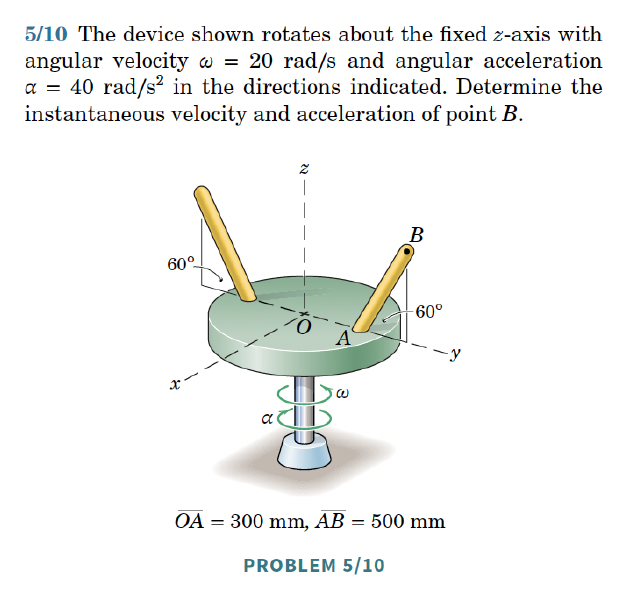
\includegraphics[width=0.5\linewidth,height=\textheight,keepaspectratio]{rigid_body_dynamics/../figures/rigid_body_kinematics/problems/05-010.png}

}

\caption{MKB 05-010.}

\end{figure}%

\textbf{2.} {[}MKB 05-013{]} \emph{(ans.
\(\mathbf{v}_A=1.121\mathbf{E}_x+0.838\mathbf{E}_y\) m/s,
\(\mathbf{a}_B=-4.48\mathbf{E}_x+0.1465\mathbf{E}_y\) m/s\(^2\))}

\begin{figure}[H]

{\centering 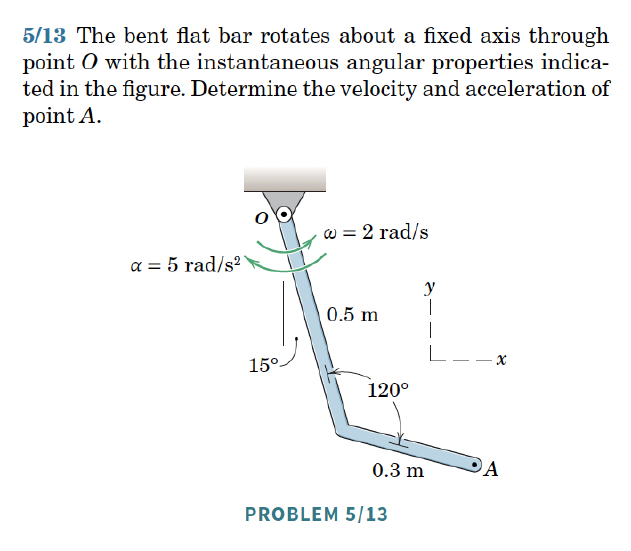
\includegraphics[width=0.5\linewidth,height=\textheight,keepaspectratio]{rigid_body_dynamics/../figures/rigid_body_kinematics/problems/05-013.png}

}

\caption{MKB 05-013.}

\end{figure}%

\textbf{3.} {[}05-018{]} \emph{(ans.
\(\mathbf{v}_A=-0.374\mathbf{E}_x+0.1905\mathbf{E}_y\) m/s,
\(\mathbf{a}_A=-0.757\mathbf{E}_x-0.605\mathbf{E}_y\) m/s\(^2\))}

\begin{figure}[H]

{\centering 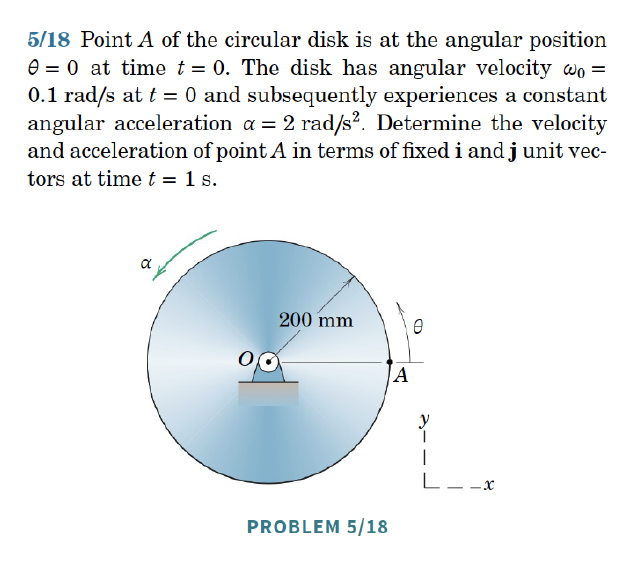
\includegraphics[width=0.5\linewidth,height=\textheight,keepaspectratio]{rigid_body_dynamics/../figures/rigid_body_kinematics/problems/05-018.png}

}

\caption{MKB 05-018.}

\end{figure}%

\textbf{4.} {[}05-049{]} \emph{(ans. (a) \(N=91.7\) rev/min CCW; (b)
\(N=45.8\) rev/min CCW; (c) \(N=45.8\) rev/min CW)}

\begin{figure}[H]

{\centering 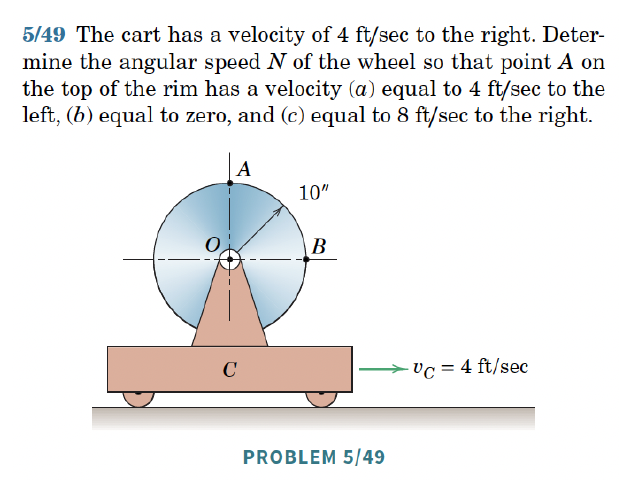
\includegraphics[width=0.5\linewidth,height=\textheight,keepaspectratio]{rigid_body_dynamics/../figures/rigid_body_kinematics/problems/05-049.png}

}

\caption{MKB 05-049.}

\end{figure}%

\textbf{5.} {[}05-065{]} \emph{(ans. \(\omega=0.722\) rad/s)}

\begin{figure}[H]

{\centering 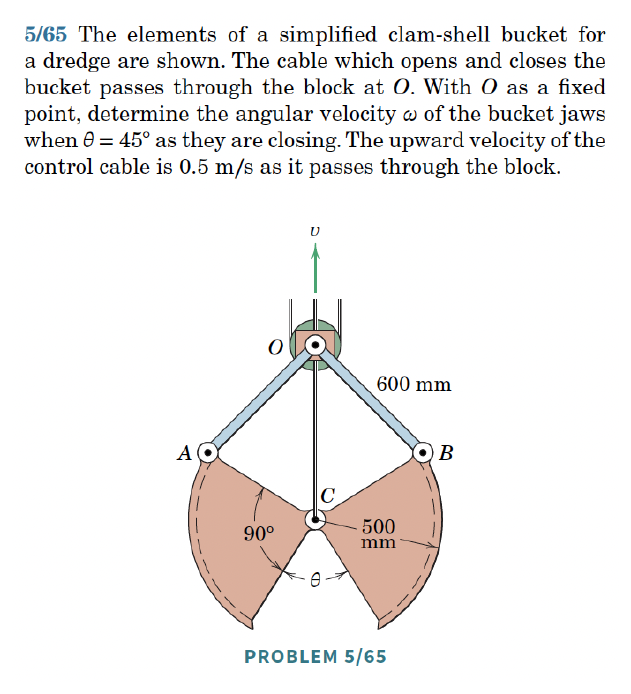
\includegraphics[width=0.5\linewidth,height=\textheight,keepaspectratio]{rigid_body_dynamics/../figures/rigid_body_kinematics/problems/05-065.png}

}

\caption{MKB 05-065.}

\end{figure}%

\textbf{6.} {[}05-069{]} \emph{(ans. \(\omega_{AB}=1.725\) rad/s CCW,
\(\omega_{BC}=4\) rad/s CCW)}

\begin{figure}[H]

{\centering 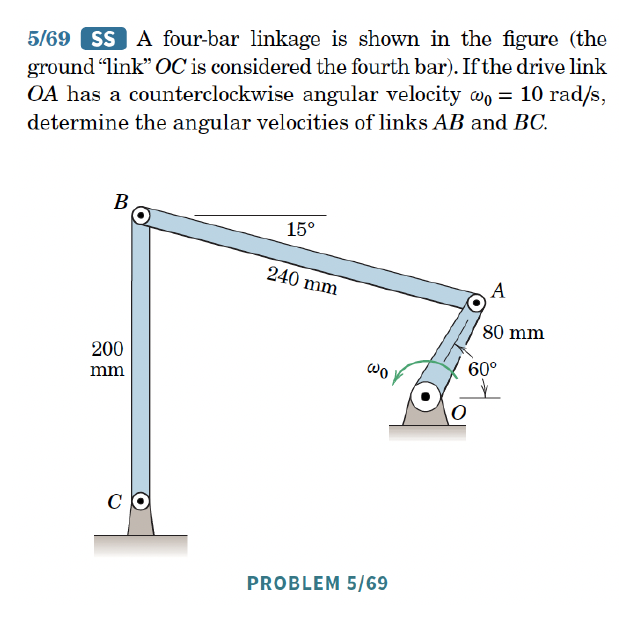
\includegraphics[width=0.5\linewidth,height=\textheight,keepaspectratio]{rigid_body_dynamics/../figures/rigid_body_kinematics/problems/05-069.png}

}

\caption{MKB 05-069.}

\end{figure}%

\subsection{Set 16 -- IC and Particle in Non-inertial
Frame}\label{set-16-ic-and-particle-in-non-inertial-frame}

\textbf{1.} {[}MKB 05-102{]} \emph{(ans. \(\alpha=0.286\) rad/s\(^2\),
\(a_A=0.653\) m/s\(^2\) down)}

\begin{figure}[H]

{\centering 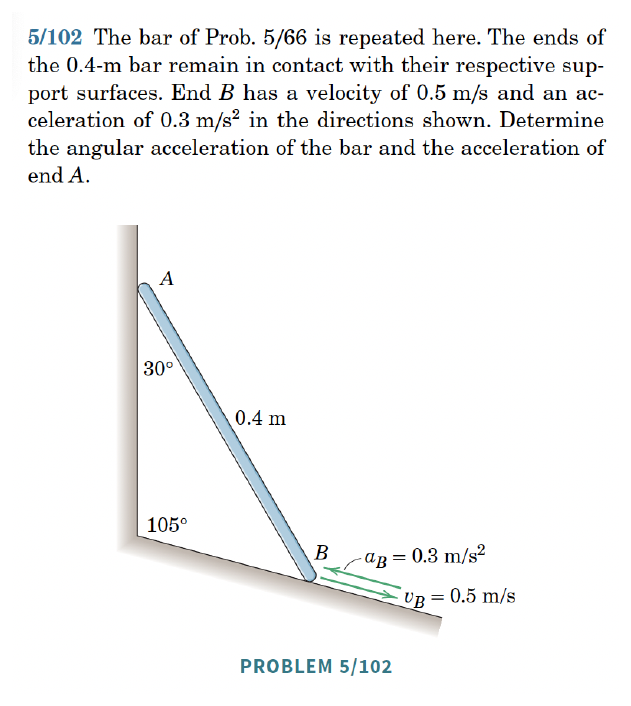
\includegraphics[width=0.5\linewidth,height=\textheight,keepaspectratio]{rigid_body_dynamics/../figures/rigid_body_kinematics/problems/05-102.png}

}

\caption{MKB 05-102.}

\end{figure}%

\url{https://youtu.be/n34Z2jwwnW0}

\textbf{2.} {[}MKB 05-125{]} \emph{(ans.
\(\mathbf{v}_A=0.1\mathbf{E}_x+0.25\mathbf{E}_y\) m/s,
\(\beta=68.2^\circ\))}

\begin{figure}[H]

{\centering 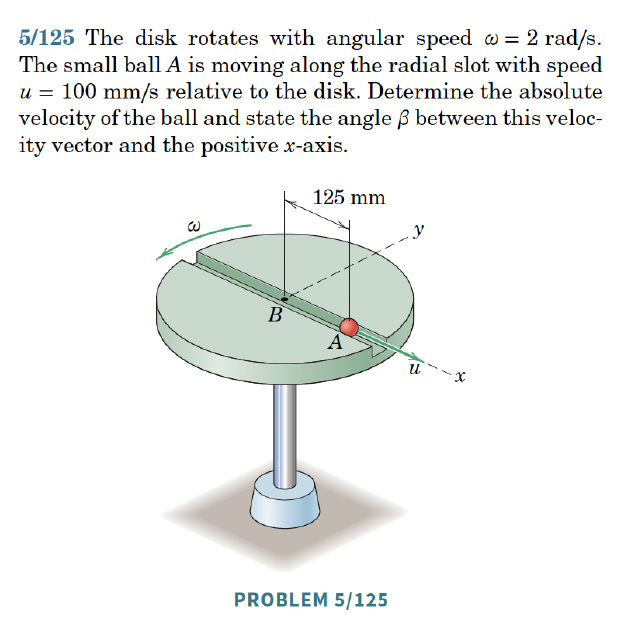
\includegraphics[width=0.5\linewidth,height=\textheight,keepaspectratio]{rigid_body_dynamics/../figures/rigid_body_kinematics/problems/05-125.png}

}

\caption{MKB 05-125.}

\end{figure}%

\url{https://youtu.be/PyM7KmlPirU}

\textbf{3.} {[}05-143{]} \emph{(ans. \(v_{\mathrm{rel}}=3.93\) m/s at
\(19.11^\circ\), \(a_{\mathrm{rel}}=15.22\) m/s\(^2\) at
\(19.11^\circ\), \(\omega_{BC}=1.429\) rad/s CW, \(\alpha_{BC}=170.0\)
rad/s\(^2\) CW)}

\begin{figure}[H]

{\centering 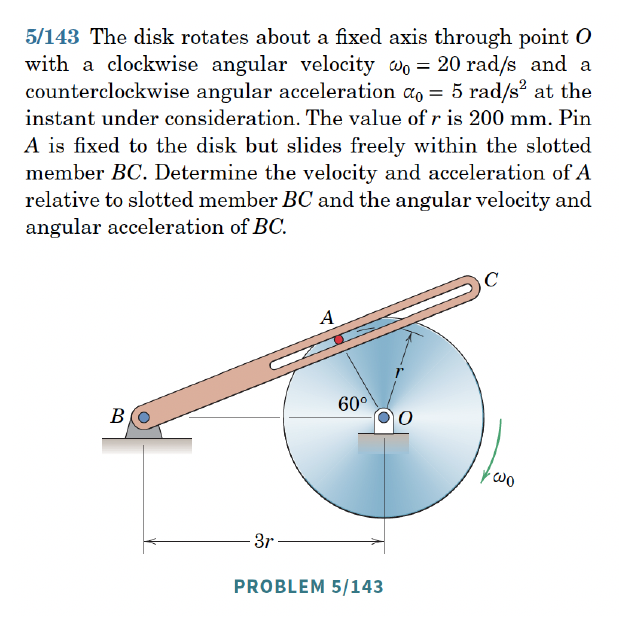
\includegraphics[width=0.5\linewidth,height=\textheight,keepaspectratio]{rigid_body_dynamics/../figures/rigid_body_kinematics/problems/05-143.png}

}

\caption{MKB 05-143.}

\end{figure}%

\url{https://youtu.be/IG7Qtj2TdFQ}

\subsection{Set 17 -- Rolling and
Sliding}\label{set-17-rolling-and-sliding}

\textbf{1.} {[}MKB 05-055{]} \emph{(ans. \(v_O=6.93\) m/s,
\(\omega=21.3\) rad/s CW)}

\begin{figure}[H]

{\centering 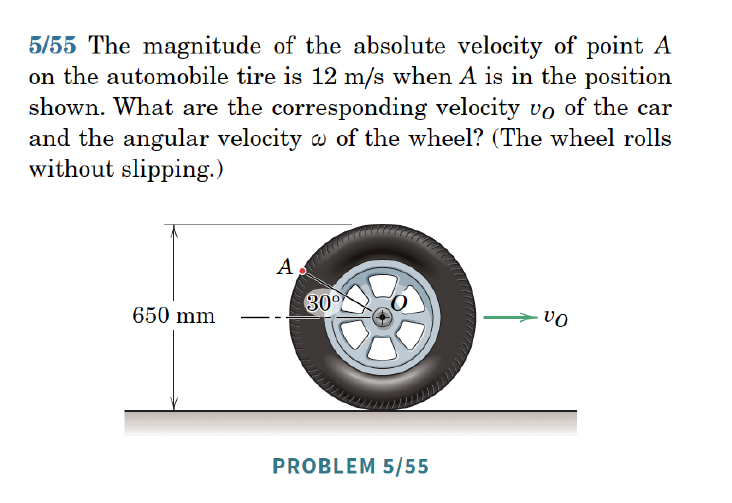
\includegraphics[width=0.5\linewidth,height=\textheight,keepaspectratio]{rigid_body_dynamics/../figures/rigid_body_kinematics/problems/05-055.png}

}

\caption{MKB 05-055.}

\end{figure}%

\textbf{2.} {[}MKB 05-087{]} \emph{(ans. \(v_O=120\) mm/s, \(v_P=216\)
mm/s)}

\begin{figure}[H]

{\centering 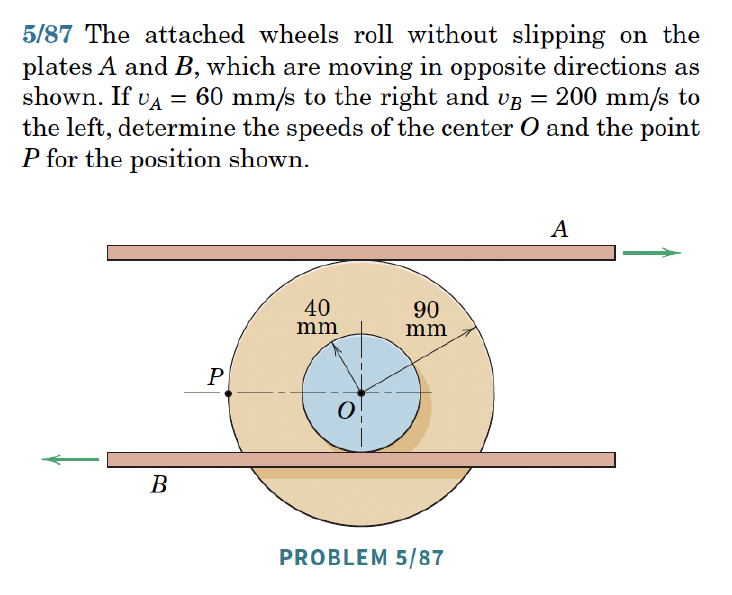
\includegraphics[width=0.5\linewidth,height=\textheight,keepaspectratio]{rigid_body_dynamics/../figures/rigid_body_kinematics/problems/05-087.png}

}

\caption{MKB 05-087.}

\end{figure}%

\textbf{3.} {[}05-091{]} \emph{(ans. \(v=15.71\) ft/s right,
\(v_s=6.89\) ft/s left)}

\begin{figure}[H]

{\centering 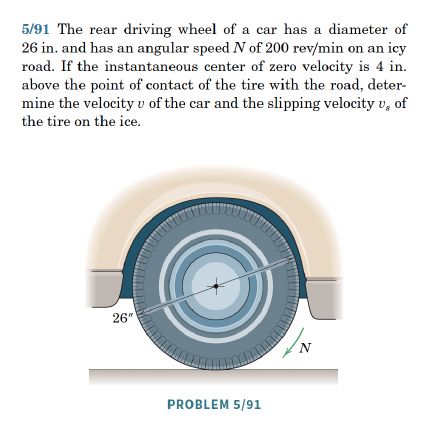
\includegraphics[width=0.5\linewidth,height=\textheight,keepaspectratio]{rigid_body_dynamics/../figures/rigid_body_kinematics/problems/05-091.png}

}

\caption{MKB 05-091.}

\end{figure}%

\textbf{4.} {[}05-093{]} \emph{(ans. \(v_A=9.19\) ft/sec left)}

\begin{figure}[H]

{\centering 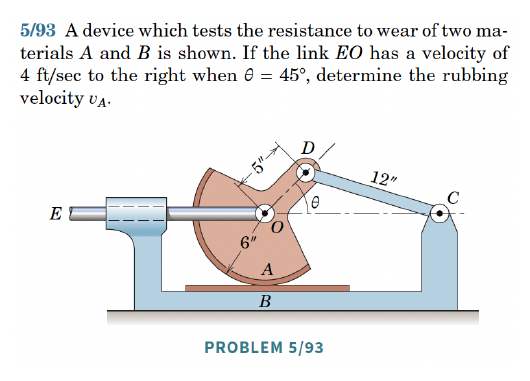
\includegraphics[width=0.5\linewidth,height=\textheight,keepaspectratio]{rigid_body_dynamics/../figures/rigid_body_kinematics/problems/05-093.png}

}

\caption{MKB 05-093.}

\end{figure}%

\textbf{5.} {[}05-100{]} \emph{(ans.
\(\mathbf{v}_A=5.12\mathbf{E}_x+2.12\mathbf{E}_y\) m/s,
\(\mathbf{a}_B=-16.25\mathbf{E}_x+2.5\mathbf{E}_y\) m/s\(^2\))}

\begin{figure}[H]

{\centering 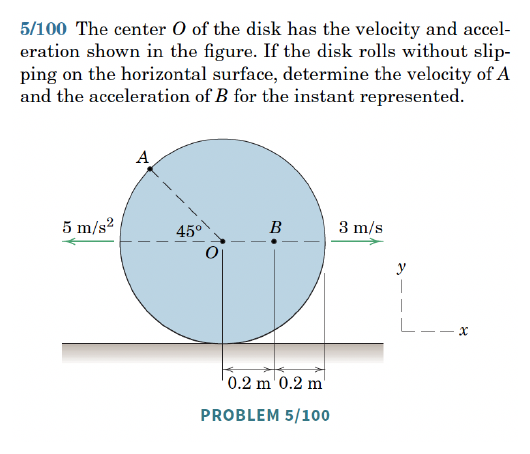
\includegraphics[width=0.5\linewidth,height=\textheight,keepaspectratio]{rigid_body_dynamics/../figures/rigid_body_kinematics/problems/05-100.png}

}

\caption{MKB 05-100.}

\end{figure}%

\subsection{Set 18 -- Moments of
Inertia}\label{set-18-moments-of-inertia}

\textbf{1.} {[}MKB B-004{]} Integration required. \emph{(ans.
\(I_{xx}=\frac{3}{10}mr^2\), \(I_{yy}=\frac{2}{5}m(r^4+h^2)/(r^2)\))}

\begin{figure}[H]

{\centering 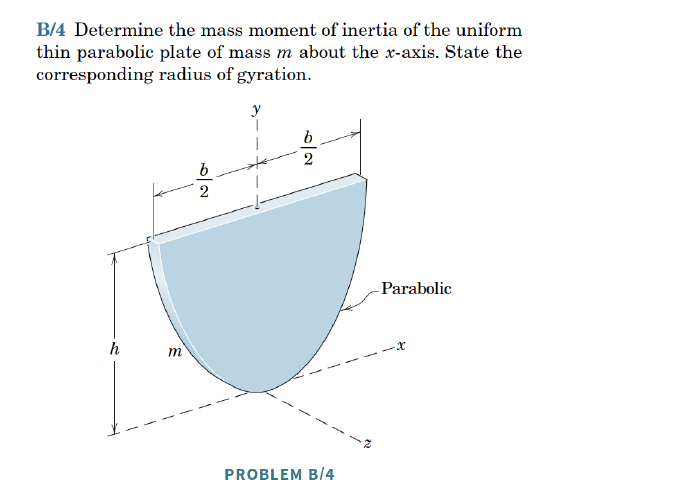
\includegraphics[width=0.5\linewidth,height=\textheight,keepaspectratio]{rigid_body_dynamics/../figures/rigid_body_kinematics/problems/B-004.png}

}

\caption{MKB B-004.}

\end{figure}%

\textbf{2.} {[}MKB B-029{]} Treat the hollow cylinder as a full cylinder
of radius \(r_2\) minus a cylinder of radius \(r_1\). \emph{(ans.
\(I_{xx}=\frac{1}{2}m(r_1^2+r_2^2)\))}

\begin{figure}[H]

{\centering 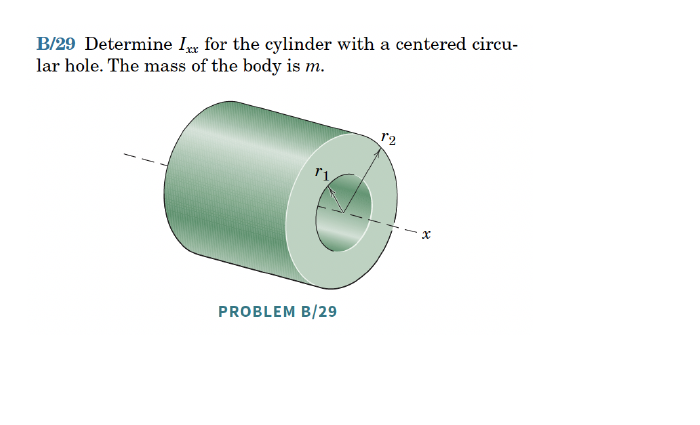
\includegraphics[width=0.5\linewidth,height=\textheight,keepaspectratio]{rigid_body_dynamics/../figures/rigid_body_kinematics/problems/B-029.png}

}

\caption{MKB B-029.}

\end{figure}%

\textbf{3.} {[}B-032{]} \emph{(ans. \(L=r\sqrt{2\sqrt{3}}\))}

\begin{figure}[H]

{\centering 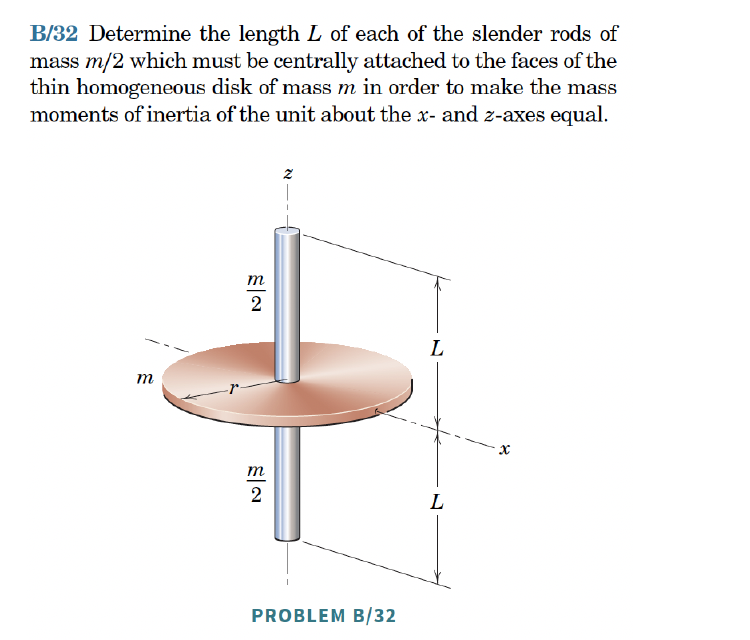
\includegraphics[width=0.5\linewidth,height=\textheight,keepaspectratio]{rigid_body_dynamics/../figures/rigid_body_kinematics/problems/B-032.png}

}

\caption{MKB B-032.}

\end{figure}%

\textbf{4.} {[}B-034{]} \emph{(ans.
\(I_{yy}=\rho L^3\left(\frac{43}{192}+\frac{83\pi}{128}\right)\))}

\begin{figure}[H]

{\centering 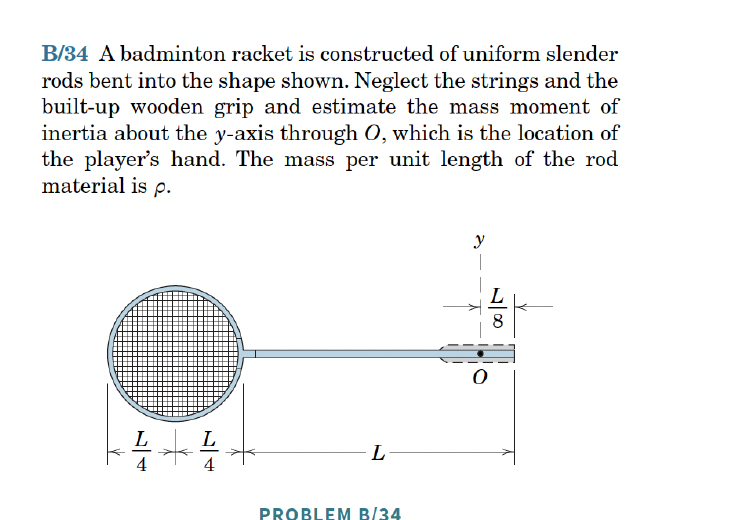
\includegraphics[width=0.5\linewidth,height=\textheight,keepaspectratio]{rigid_body_dynamics/../figures/rigid_body_kinematics/problems/B-034.png}

}

\caption{MKB B-034.}

\end{figure}%

\chapter{Kinetics of Rigid Bodies}\label{kinetics-of-rigid-bodies}

\section{Balance Laws for a Rigid
Body}\label{balance-laws-for-a-rigid-body}

The balance laws for a rigid body are \textbf{Euler's first law}
(Balance of Linear Momentum, BoLM) \begin{align}
    {\bf F} &= m{\bf a}_C,
\end{align} and \textbf{Euler's second law} (Balance of Angular
Momentum, BoAM), which can be expressed in three equivalent forms:
\begin{align}
    {\bf M}^O &= \dot{\bf H}^O \quad\text{about a fixed point }O,\\
    {\bf M}^C &= \dot{\bf H}^C \quad\text{about the center of mass }C,\\
    {\bf M}^P &= \dot{\bf H}^P+({\bf v}_P-{\bf v}_C)\times{\bf G} = \dot{\bf H}^C+({\bf r}_C-{\bf r}_P)\times m{\bf a}_C \quad\text{about any material point }P.
\end{align} The BoAM is an \textbf{independent postulate}, not derivable
from the BoLM.

\section{Resultant Forces and
Moments}\label{resultant-forces-and-moments}

The resultant force \({\bf F}\) is the sum of all external forces. The
resultant moment about a point includes the moment due to forces plus
any applied pure moments \({\bf M}_e\) not due to forces.

\begin{center}
\pandocbounded{
\includegraphics[keepaspectratio]{rigid_body_dynamics/rigid_body_kinetics_files/figure-pdf/unnamed-chunk-1-1.pdf}}
\end{center}

For \(K\) forces \({\bf F}_i\) acting at positions \({\bf r}_i\) plus a
pure moment \({\bf M}_e\): \begin{align}
    {\bf F} &= \sum_{i=1}^K{\bf F}_i,\\
    {\bf M}^O &= {\bf M}_e+\sum_{i=1}^K{\bf r}_i\times{\bf F}_i,\\
    {\bf M}^C &= {\bf M}_e+\sum_{i=1}^K({\bf r}_i-{\bf r}_C)\times{\bf F}_i.
\end{align}

Examples of pure moments: reaction moments \({\bf M}_R\) at joints;
torsional spring moments \(-K_T(\theta-\theta_0){\bf E}_z\).

\url{https://www.youtube.com/watch?v=Era7OOKyVEw}

\subsection{Does Weight Result in a Moment About the Center of
Mass?}\label{does-weight-result-in-a-moment-about-the-center-of-mass}

The total weight is
\({\bf W} = \int_{\mathcal{B}}{\bf g}\,dm = {\bf g}\int_{\mathcal{B}}dm = m{\bf g}\),
and its moment about \(C\) is: \begin{align}
    {\bf M}^C = \int_{\mathcal{B}}\bpi\times{\bf g}\,dm = \lp\int_{\mathcal{B}}\bpi\,dm\rp\times{\bf g} = {\bf 0},
\end{align} since \(\int_{\mathcal{B}}\bpi\,dm = {\bf 0}\) by definition
of the center of mass.

\section{Equivalence of the BoAM
Forms}\label{equivalence-of-the-boam-forms}

The following devepments are true for rigid bodies where the inertia
matrix is constant in the body frame.

\subsection{\texorpdfstring{BoAM About Any Point
\(P\)}{BoAM About Any Point P}}\label{boam-about-any-point-p}

Starting from \({\bf M}^C = \dot{\bf H}^C\) and replacing
\({\bf M}^P = {\bf M}^C+({\bf r}_C-{\bf r}_P)\times{\bf F}\):
\begin{align}
    {\bf M}^P = \dot{\bf H}^C+({\bf r}_C-{\bf r}_P)\times{\bf F}.
\end{align} Substituting
\(\dot{\bf H}^C = \dot{\bf H}^P+({\bf v}_P-{\bf v}_C)\times{\bf G}+({\bf r}_P-{\bf r}_C)\times m{\bf a}_C\)
and simplifying: \begin{align}
    \begin{split}
        {\bf M}^P &= \dot{\bf H}^P+({\bf v}_P-{\bf v}_C)\times{\bf G}+({\bf r}_P-{\bf r}_C)\times m{\bf a}_C+({\bf r}_C-{\bf r}_P)\times{\bf F},\\
        &= \dot{\bf H}^P+({\bf v}_P-{\bf v}_C)\times{\bf G},
    \end{split}
\end{align} recovering the BoAM about a general material point \(P\).

\subsection{\texorpdfstring{BoAM About a Fixed Point
\(O\)}{BoAM About a Fixed Point O}}\label{boam-about-a-fixed-point-o}

If \(P\) is a fixed point \(O\) (so \({\bf v}_O = {\bf 0}\)), the above
simplifies to \({\bf M}^O = \dot{\bf H}^O\).

\begin{tcolorbox}[enhanced jigsaw, arc=.35mm, bottomrule=.15mm, bottomtitle=1mm, breakable, colback=white, colbacktitle=quarto-callout-tip-color!10!white, colframe=quarto-callout-tip-color-frame, coltitle=black, left=2mm, leftrule=.75mm, opacityback=0, opacitybacktitle=0.6, rightrule=.15mm, title=\textcolor{quarto-callout-tip-color}{\faLightbulb}\hspace{0.5em}{Think!}, titlerule=0mm, toprule=.15mm, toptitle=1mm]

\textbf{Question:} When is the angular momentum of a rigid body about a
fixed point \(O\) or about its center of mass \(C\) conserved? Under
what conditions are these anguar momenta conserved in a certain
direction (eg. along \({\bf E}_z\))?

\begin{quote}
\textbf{Answer}

\url{https://www.youtube.com/shorts/VmeM0BNnGR0}

\url{https://www.youtube.com/watch?v=64t-dVtDwkQ}
\end{quote}

\end{tcolorbox}

\section{Calculating the Derivative of Angular
Momentum}\label{calculating-the-derivative-of-angular-momentum}

Recall that \begin{align}
    \begin{split}
        {\bf H}^P = {\bf I}^P\bomega+({\bf r}_C-{\bf r}_P)\times m{\bf v}_P
    \end{split}
\end{align} if \(P\) is taken to be the center of mass \(C\) or a fixed
point \(O\) respectively, we get \begin{align}
    \begin{split}
        {\bf H}^C = {\bf I}^C\bomega,\\
        {\bf H}^P = {\bf I}^P\bomega.
    \end{split}
\end{align} In component form, \begin{align}
    {\bf H}^C = (I_{xx}^C\omega_x+I_{xy}^C\omega_y+I_{xz}^C\omega_z){\bf e}_x+(I_{xy}^C\omega_x+I_{yy}^C\omega_y+I_{yz}^C\omega_z){\bf e}_y+(I_{xz}^C\omega_x+I_{yz}^C\omega_y+I_{zz}^C\omega_z){\bf e}_z.
\end{align} where \begin{align}
    \bomega = \omega_x{\bf e}_x+\omega_y{\bf e}_y+\omega_z{\bf e}_z.
\end{align} We need to calculate \(\dot{\bf H}^C\). \begin{align}
    \dot{\bf H}^C=\overset{\circ}{{\bf H}^C}+\bomega\times{\bf H}^C.
\end{align} where \(\overset{\circ}{{\bf H}^C}\) is the corotational
rate of \({\bf H}\), that is the time derivative of \({\bf H}\) that is
obtained while keeping \({\bf e}_x\), \({\bf e}_y\), and \({\bf e}_z\)
fixed: \begin{align}
    \overset{\circ}{{\bf H}^C} = (I_{xx}^C\dot{\omega}_x+I_{xy}^C\dot{\omega}_y+I_{xz}^C\dot{\omega}_z){\bf e}_x+(I_{xy}^C\dot{\omega}_x+I_{yy}^C\dot{\omega}_y+I_{yz}^C\dot{\omega}_z){\bf e}_y+(I_{xz}^C\dot{\omega}_x+I_{yz}^C\dot{\omega}_y+I_{zz}^C\dot{\omega}_z){\bf e}_z.
\end{align} For the case where \(\bomega=\omega{\bf E}_z\) considered
exclusively in this class, the previous expressions simplify to
\begin{align}
    \begin{split}
        {\bf H}^C &= I_{xz}^C\omega_z{\bf e}_x+I_{yz}^C\omega_z{\bf e}_y+I_{zz}^C\omega_z{\bf e}_z,\\
        \dot{\bf H}^C &= (I_{xz}^C\dot{\omega}-I_{yz}^C\omega^2){\bf e}_x+(I_{yz}^C\dot{\omega}+I_{xz}^C\omega^2){\bf e}_y+I_{zz}^C\dot{\omega}{\bf E}_z.
    \end{split}
\end{align} Analogous developments yield \begin{align}
    \begin{split}
        & \dot{\bf H}^O = (I_{xz}^O\dot{\omega}-I_{yz}^O\omega^2){\bf e}_x+(I_{yz}^O\dot{\omega}+I_{xz}^O\omega^2){\bf e}_y+I_{zz}^O\dot{\omega}{\bf E}_z,\\
        & \dot{\bf H}^C = (I_{xz}^C\dot{\omega}-I_{yz}^C\omega^2){\bf e}_x+(I_{yz}^C\dot{\omega}+I_{xz}^C\omega^2){\bf e}_y+I_{zz}^C\dot{\omega}{\bf E}_z,\\
        & \dot{\bf H}^P = (I_{xz}^P\dot{\omega}-I_{yz}^P\omega^2){\bf e}_x+(I_{yz}^P\dot{\omega}+I_{xz}^P\omega^2){\bf e}_y+I_{zz}^P\dot{\omega}{\bf E}_z+\frac{d}{dt}\left(({\bf r}_C-{\bf r}_P)\times m{\bf v}_P\right).
    \end{split}
\end{align} For fixed axis rotation, it is generally better to sum the
moments about a fixed point passing through the axis of rotation. For
general plane motion, there is no fixed point, so the BoAM is either
summed about the center of mass or about a general material point \(P\)
on the body.

\begin{tcolorbox}[enhanced jigsaw, arc=.35mm, bottomrule=.15mm, bottomtitle=1mm, breakable, colback=white, colbacktitle=quarto-callout-important-color!10!white, colframe=quarto-callout-important-color-frame, coltitle=black, left=2mm, leftrule=.75mm, opacityback=0, opacitybacktitle=0.6, rightrule=.15mm, title=\textcolor{quarto-callout-important-color}{\faExclamation}\hspace{0.5em}{Note!}, titlerule=0mm, toprule=.15mm, toptitle=1mm]

Remember, the BoAM about a general point has additional terms to
\({\bf I}^P\bomega\): \begin{align}
    \begin{split}
        {\bf M}^P &= (I_{xz}^P\dot{\omega}-I_{yz}^P\omega^2){\bf e}_x+(I_{yz}^P\dot{\omega}+I_{xz}^P\omega^2){\bf e}_y+I_{zz}^P\dot{\omega}{\bf E}_z+({\bf v}_P-{\bf v}_C)\times{\bf G},\\
        &= (I_{xz}^C\dot{\omega}-I_{yz}^C\omega^2){\bf e}_x+(I_{yz}^C\dot{\omega}+I_{xz}^C\omega^2){\bf e}_y+I_{zz}^C\dot{\omega}{\bf E}_z + ({\bf r}_C-{\bf r}_P)\times m{\bf a}_C.
    \end{split}
\end{align}

\end{tcolorbox}

\section{Impact Problems and Center of
Percussion}\label{impact-problems-and-center-of-percussion}

For rigid bodies, impact ideas are the same as in systems of particles.

\emph{Example:} Consider a projectile fired horizontally at a pendulum
(in the horizontal plane, no gravity). Find position \(x\) along the
pendulum such that the reaction force at the pin is nearly zero during
impact. If \(x\) is large, the horizontal reaction at \(O\) points left;
if \(x\) is small, it points right. The optimal \(x\) that minimizes the
reaction is called the \textbf{center of percussion}.

\begin{center}
\pandocbounded{
\includegraphics[keepaspectratio]{rigid_body_dynamics/rigid_body_kinetics_files/figure-pdf/unnamed-chunk-2-1.pdf}}
\end{center}

\section{Impulse and Momentum for Rigid
Bodies}\label{impulse-and-momentum-for-rigid-bodies}

The \textbf{linear impulse - linear momentum equation} is \begin{align}
    \int_{t_A}^{t^B}{\bf F}dt = {\bf G}(t_B)-{\bf G}(t_A).
\end{align} The \textbf{angular impulse - angular momentum equations}
are equivalently \begin{align}
    & \int_{t_A}^{t_B}{\bf M}^C dt = {\bf H}^C(t_B)-{\bf H}^C(t_A)\quad\text{where $C$ is the center of mass},\\
    & \int_{t_A}^{t_B}{\bf M}^O dt = {\bf H}^O(t_B)-{\bf H}^O(t_A)\quad\text{if there is a fixed point }O.
\end{align}

\section{Moment-Free Motion of a Rigid
Body}\label{moment-free-motion-of-a-rigid-body}

The Tennis Racket Problem: A tennis racket is thrown in the air with a
certain angular velocity. The racket rotates about its center of mass,
and the angular momentum is conserved. The racket has three principal
axes of rotation, and the stability of rotation depends on which axis is
used. Rotation about the axis with the largest or smallest moment of
inertia is stable, while rotation about the intermediate axis is
unstable.

This is also known as the Dzhanibekov effect.

You can learn more about this
\href{https://rotations.berkeley.edu/a-tumbling-t-handle-in-space/}{here}
and
\href{https://rotations.berkeley.edu/a-book-tossed-in-the-air/}{here}.

https://www.youtube.com/watch?v=1VPfZ\_XzisU\&t=22s

\url{https://www.youtube.com/watch?v=1VPfZ_XzisU&t=22s}

\section{Summary}\label{summary-12}

For \(K\) forces and a moment \({\bf M}_e\) acting on a rigid body, the
balance laws are: \begin{align}
    {\bf F} = m\frac{d{\bf v}_C}{dt}, \qquad {\bf M}^O = \dot{\bf H}^O \quad (\text{or equivalently } {\bf M}^C = \dot{\bf H}^C).
\end{align}

For fixed-axis rotation with \(\bomega = \omega{\bf E}_z\) and
\(I_{xz}=I_{yz}=0\): \begin{align}
    {\bf F} = m\dot{\bf v}_C, \qquad {\bf M} = I_{zz}\dot{\omega}{\bf E}_z.
\end{align}

Four classes of applications: (1) purely translational motion
(\(\bomega=\balpha={\bf 0}\)), (2) rigid body with a fixed point, (3)
rolling and sliding rigid bodies, (4) imbalanced rotors.

It is important to note that for the second set of applications, the
balance law \({\bf M}^O=\dot{\bf H}^O\) is more convenient to use than
\({\bf M}=\dot{\bf H}\). The role of \({\bf M}_R\) in these problems is
to ensure that the axis of rotation remains \({\bf E}_z\). Finally, the
four steps discussed are used as a guide to solving all of the
applications.

\section{Exercises}\label{exercises-15}

\subsection{Set 19 -- Rigid Body
Translation}\label{set-19-rigid-body-translation}

\textbf{1.} {[}MKB 06-006{]} \emph{(ans. \(a=5.66\) m/s\(^2\))}

\begin{figure}[H]

{\centering 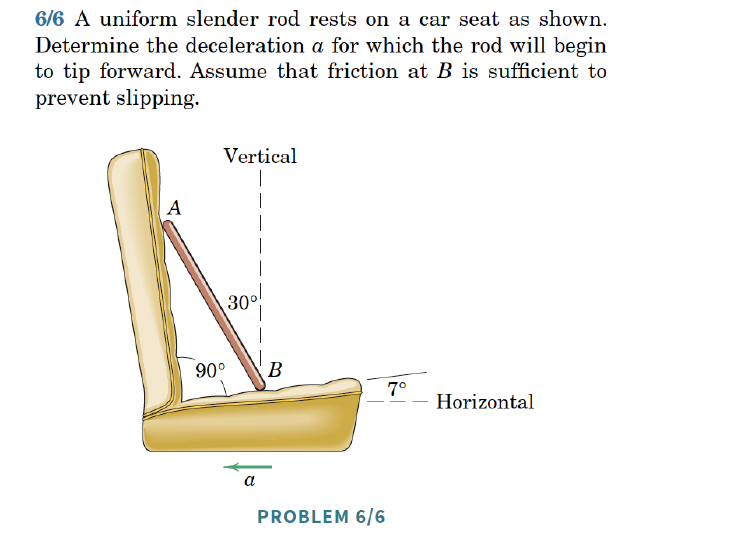
\includegraphics[width=0.5\linewidth,height=\textheight,keepaspectratio]{rigid_body_dynamics/../figures/rigid_body_kinetics/problems/06-006.png}

}

\caption{MKB 06-006.}

\end{figure}%

\textbf{2.} {[}06-012{]} \emph{(ans. \(a=16.43\) ft/sec\(^2\))}

\begin{figure}[H]

{\centering 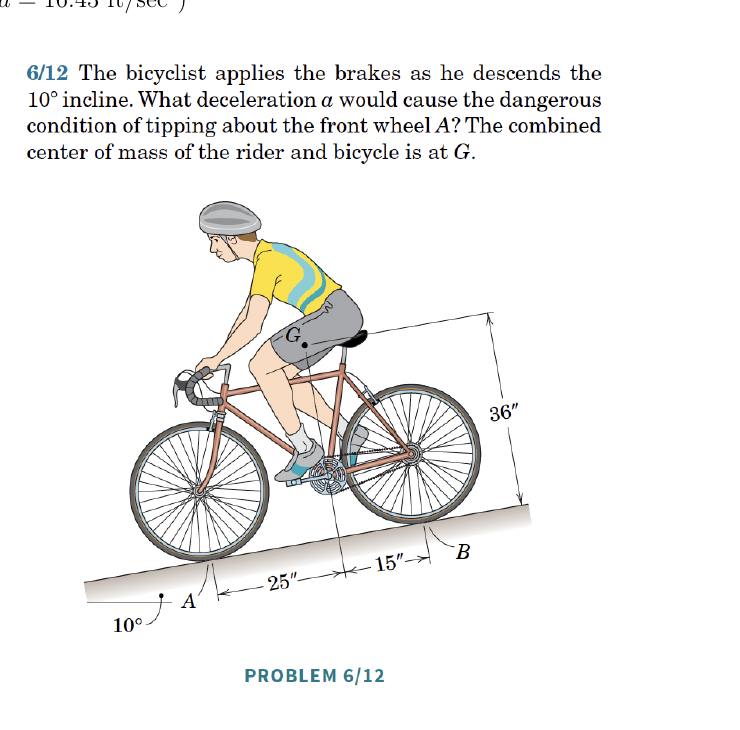
\includegraphics[width=0.5\linewidth,height=\textheight,keepaspectratio]{rigid_body_dynamics/../figures/rigid_body_kinetics/problems/06-012.png}

}

\caption{MKB 06-012.}

\end{figure}%

\textbf{3.} {[}06-013{]} \emph{(ans. \(N_A=6.85\) kN up, \(N_B=9.34\) kN
up)}

\begin{figure}[H]

{\centering 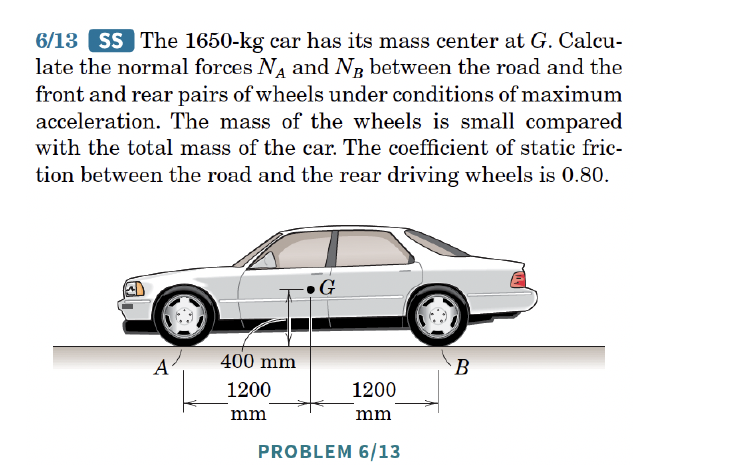
\includegraphics[width=0.5\linewidth,height=\textheight,keepaspectratio]{rigid_body_dynamics/../figures/rigid_body_kinetics/problems/06-013.png}

}

\caption{MKB 06-013.}

\end{figure}%

\textbf{4.} {[}06-022{]} \emph{(ans. \(N=257\) kN up)}

\begin{figure}[H]

{\centering 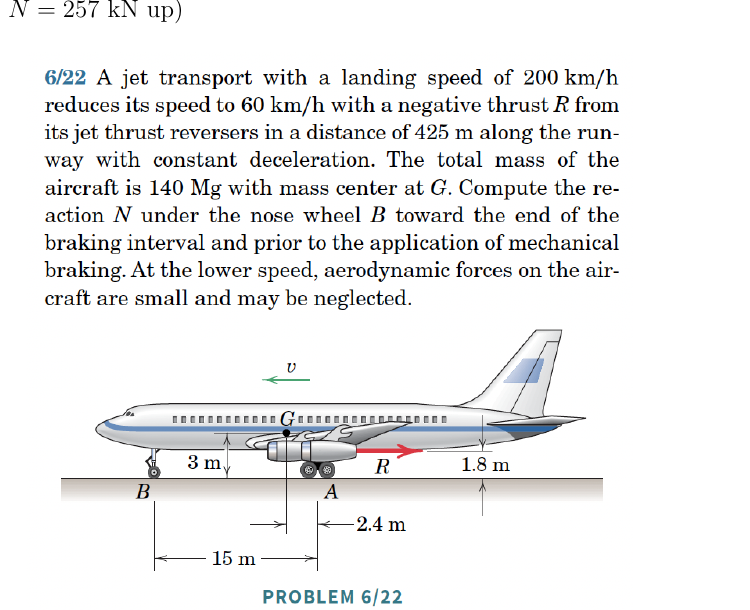
\includegraphics[width=0.5\linewidth,height=\textheight,keepaspectratio]{rigid_body_dynamics/../figures/rigid_body_kinetics/problems/06-022.png}

}

\caption{MKB 06-022.}

\end{figure}%

\subsection{Set 20 -- Fixed Point
Rotation}\label{set-20-fixed-point-rotation}

\textbf{1.} {[}MKB 06-029{]} \emph{(ans. \(\alpha=1.193\) rad/s\(^2\)
CCW, \(F_A=769\) N)}

\begin{figure}[H]

{\centering 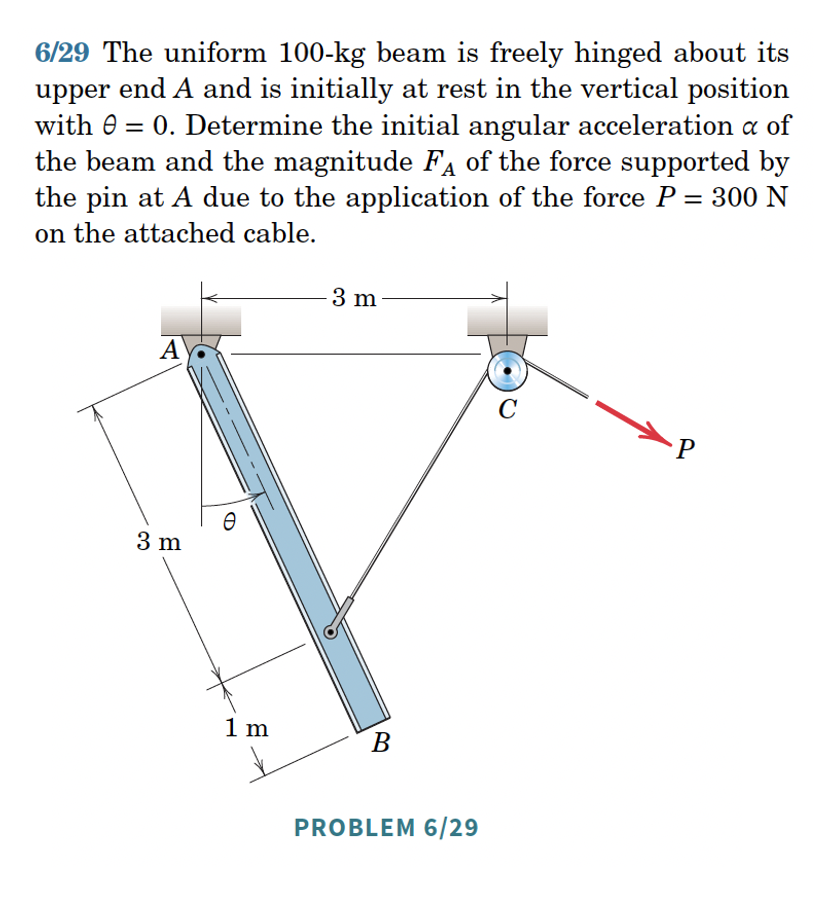
\includegraphics[width=0.5\linewidth,height=\textheight,keepaspectratio]{rigid_body_dynamics/../figures/rigid_body_kinetics/problems/06-029.png}

}

\caption{MKB 06-029.}

\end{figure}%

\textbf{2.} {[}MKB 06-035{]} \emph{(ans. \(R=3.57\) lb)}

\begin{figure}[H]

{\centering 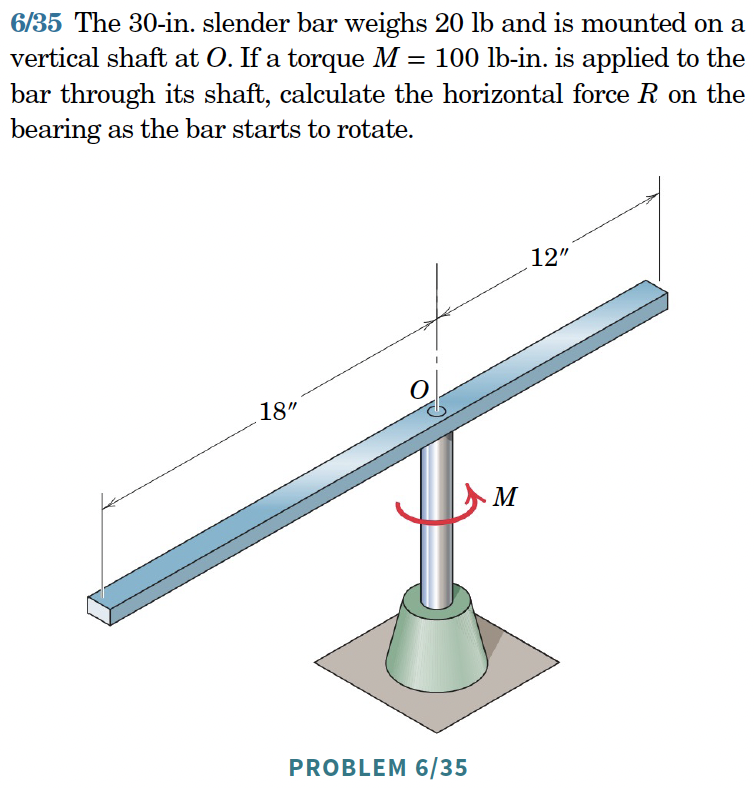
\includegraphics[width=0.5\linewidth,height=\textheight,keepaspectratio]{rigid_body_dynamics/../figures/rigid_body_kinetics/problems/06-035.png}

}

\caption{MKB 06-035.}

\end{figure}%

\url{https://youtu.be/gvBZyEq_bGo}

\textbf{3.} {[}06-037{]} \emph{(ans. \(A=56.3\) N)}

\begin{figure}[H]

{\centering 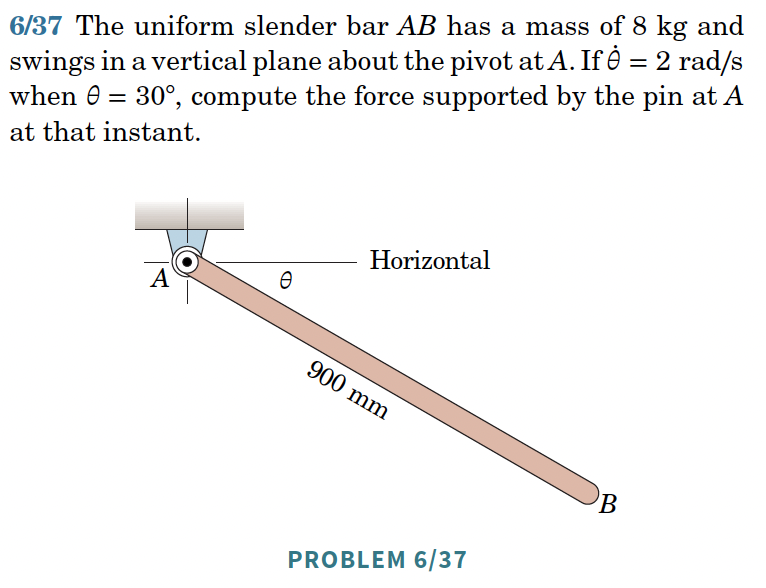
\includegraphics[width=0.5\linewidth,height=\textheight,keepaspectratio]{rigid_body_dynamics/../figures/rigid_body_kinetics/problems/06-037.png}

}

\caption{MKB 06-037.}

\end{figure}%

\textbf{4.} {[}06-039{]} \emph{(ans. (a) \(\alpha=7.85\) rad/s\(^2\)
CCW, (b) \(\alpha=6.28\) rad/s\(^2\) CCW)}

\begin{figure}[H]

{\centering 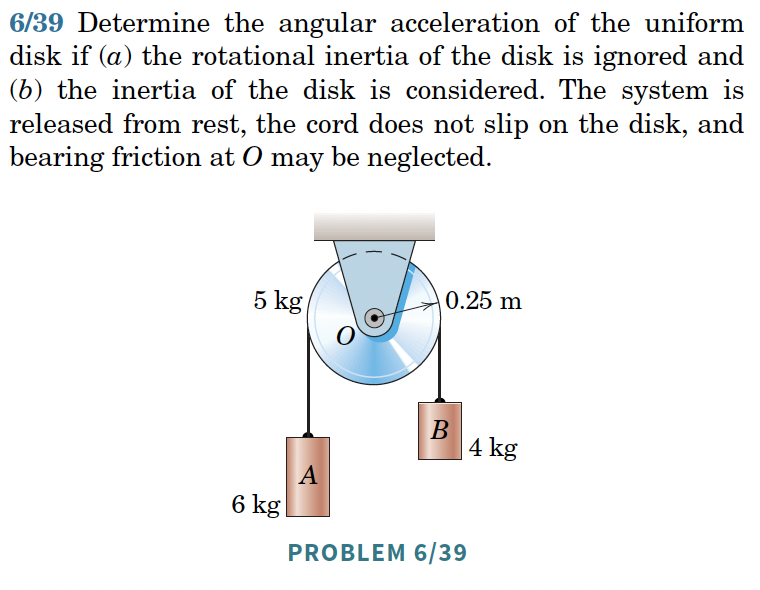
\includegraphics[width=0.5\linewidth,height=\textheight,keepaspectratio]{rigid_body_dynamics/../figures/rigid_body_kinetics/problems/06-039.png}

}

\caption{MKB 06-039.}

\end{figure}%

\textbf{5.} {[}06-051{]} \emph{(ans. \(b=40.7\) mm, \(R=167.8\) N)}

\begin{figure}[H]

{\centering 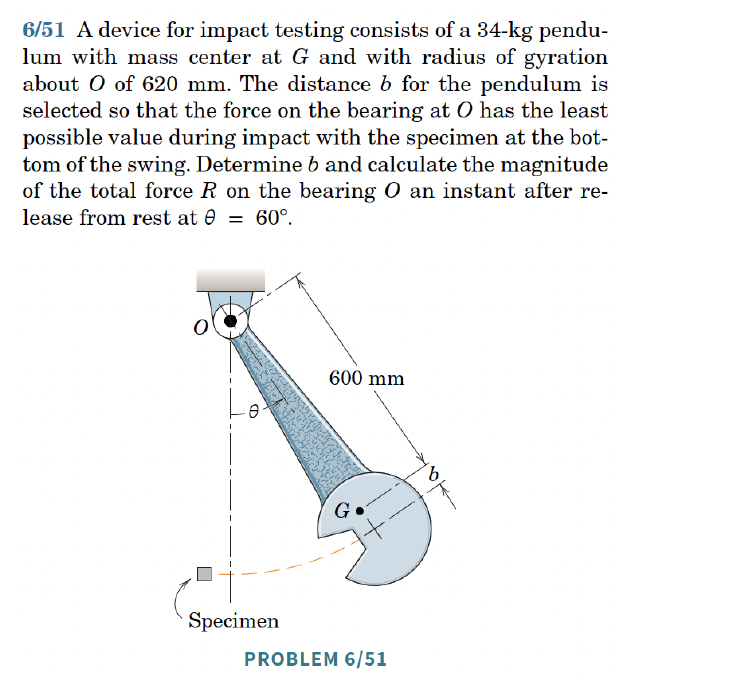
\includegraphics[width=0.5\linewidth,height=\textheight,keepaspectratio]{rigid_body_dynamics/../figures/rigid_body_kinetics/problems/06-051.png}

}

\caption{MKB 06-051.}

\end{figure}%

\url{https://youtu.be/Q7PV2pxBuwc}

\textbf{6.} {[}06-054{]} \emph{(ans.
\(\alpha=\frac{6g}{7l}-\frac{12k}{7m}(\sqrt{5}-\sqrt{3})\))}

\begin{figure}[H]

{\centering 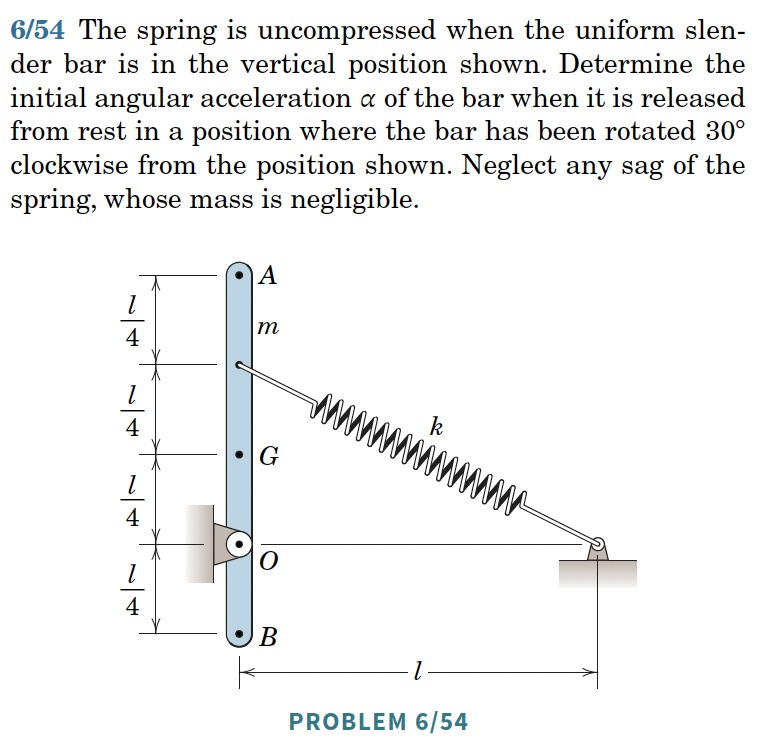
\includegraphics[width=0.5\linewidth,height=\textheight,keepaspectratio]{rigid_body_dynamics/../figures/rigid_body_kinetics/problems/06-054.png}

}

\caption{MKB 06-054.}

\end{figure}%

\textbf{7.} {[}MKB 07-066{]} \emph{Dynamic imbalance of a rotating shaft
carrying two offset point masses.}

\begin{figure}[H]

{\centering 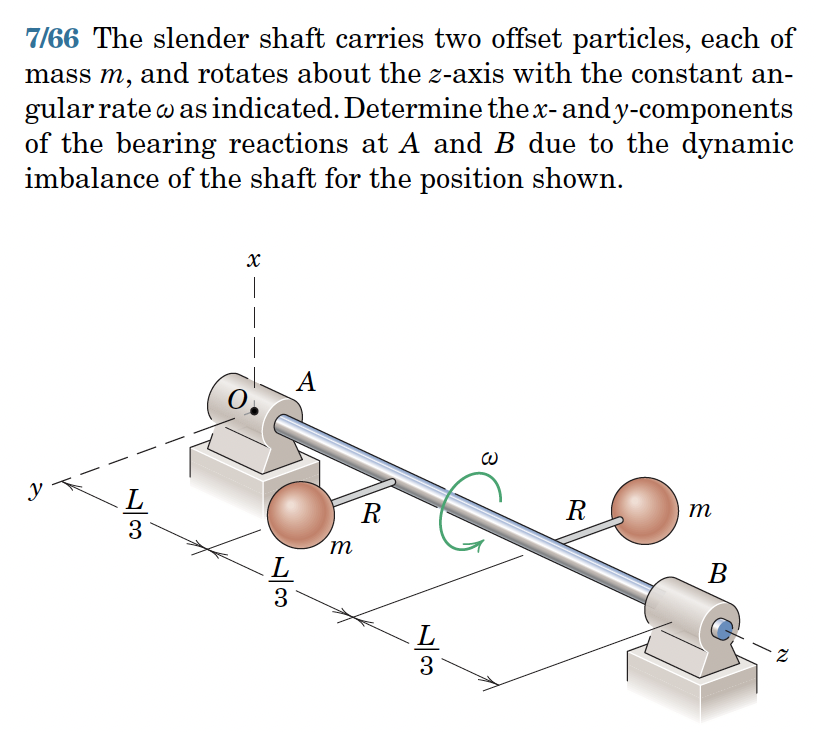
\includegraphics[width=0.5\linewidth,height=\textheight,keepaspectratio]{rigid_body_dynamics/../figures/rigid_body_kinetics/problems/07-066.png}

}

\caption{MKB 07-066.}

\end{figure}%

\url{https://youtu.be/HGiVnQbItTI}

\subsection{Set 21 -- General Plane
Motion}\label{set-21-general-plane-motion}

\textbf{1.} {[}MKB 06-061{]} \emph{(ans. \(\alpha=48.8\) rad/s\(^2\) CW,
\(\bar a_x=0\), \(\bar a_y=5\) m/s\(^2\))}

\begin{figure}[H]

{\centering 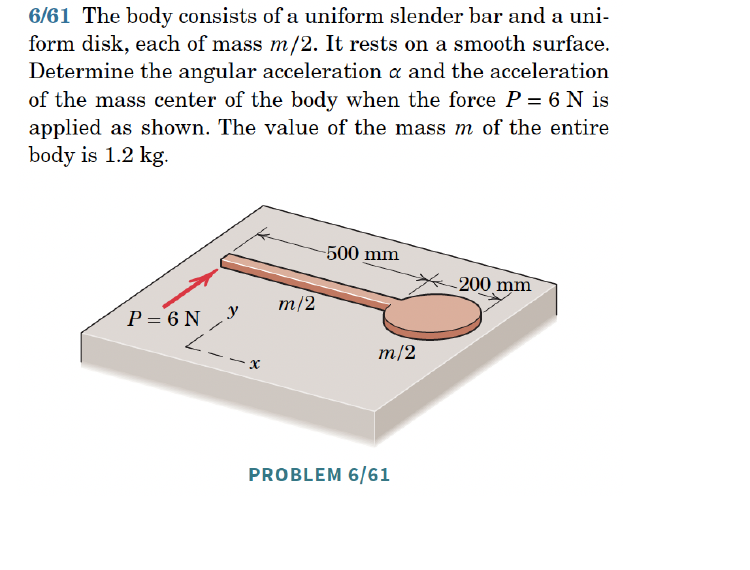
\includegraphics[width=0.5\linewidth,height=\textheight,keepaspectratio]{rigid_body_dynamics/../figures/rigid_body_kinetics/problems/06-061.png}

}

\caption{MKB 06-061.}

\end{figure}%

\textbf{2.} {[}MKB 06-062{]} \emph{(ans. A:
\(\alpha_A=\frac{g}{r}\sin\theta\), \(\mu_s=0\); B:
\(\alpha_B=\frac{g}{2r}\sin\theta\), \(\mu_s=\frac{1}{2}\tan\theta\))}

\begin{figure}[H]

{\centering 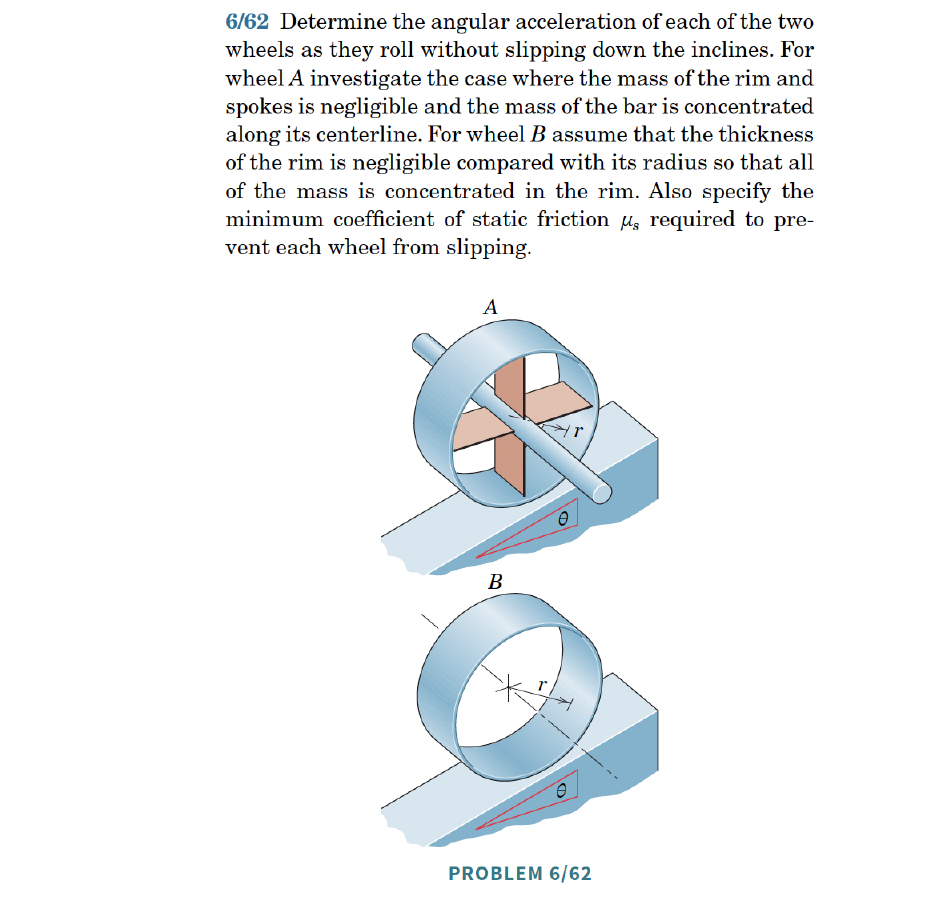
\includegraphics[width=0.5\linewidth,height=\textheight,keepaspectratio]{rigid_body_dynamics/../figures/rigid_body_kinetics/problems/06-062.png}

}

\caption{MKB 06-062.}

\end{figure}%

\textbf{3.} {[}06-063{]} \emph{(ans. \(\bar a=13.80\) ft/sec\(^2\) down
incline, \(F=1.714\) lb up incline)}

\begin{figure}[H]

{\centering 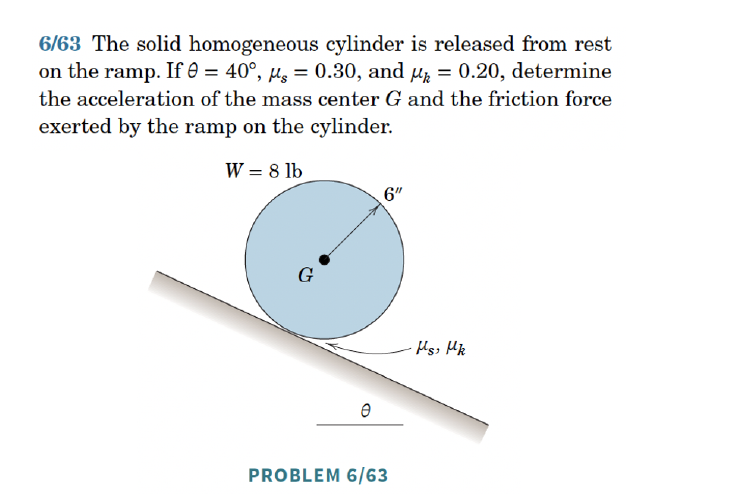
\includegraphics[width=0.5\linewidth,height=\textheight,keepaspectratio]{rigid_body_dynamics/../figures/rigid_body_kinetics/problems/06-063.png}

}

\caption{MKB 06-063.}

\end{figure}%

\textbf{4.} {[}06-070{]} \emph{(ans. \(a=\frac{8(m+M)g}{3\pi(m+3M)}\)
left, \(\alpha=\frac{8mg}{3\pi r(m+3M)}\) CW)}

\begin{figure}[H]

{\centering 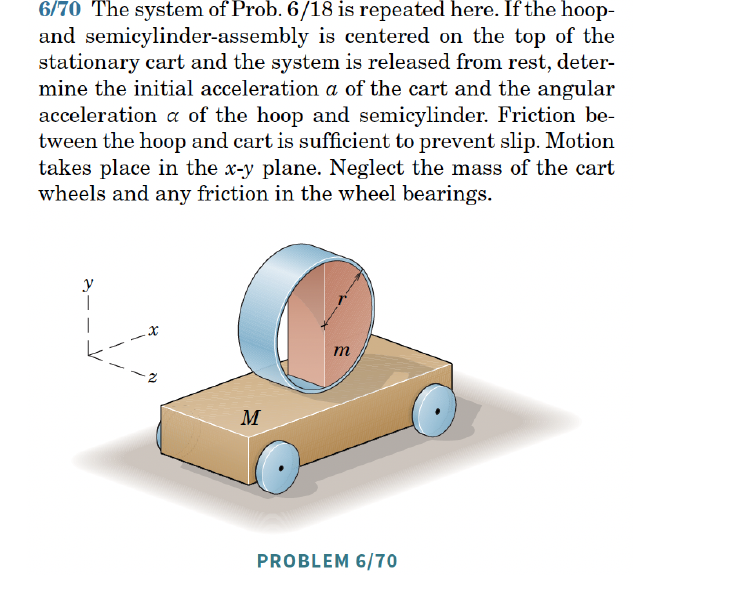
\includegraphics[width=0.5\linewidth,height=\textheight,keepaspectratio]{rigid_body_dynamics/../figures/rigid_body_kinetics/problems/06-070.png}

}

\caption{MKB 06-070.}

\end{figure}%

\url{https://youtu.be/3UvEbjlaBwc}

\textbf{5.} {[}06-076{]} \emph{(ans. \(s=\frac{3d}{2}\))}

\begin{figure}[H]

{\centering 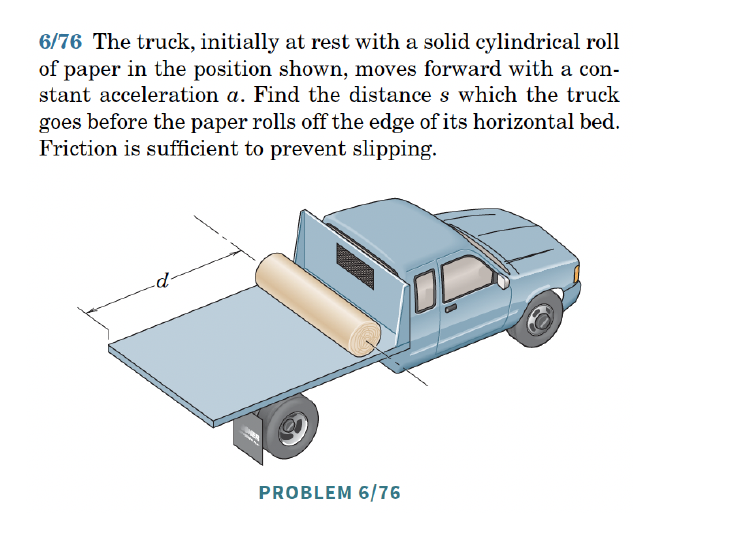
\includegraphics[width=0.5\linewidth,height=\textheight,keepaspectratio]{rigid_body_dynamics/../figures/rigid_body_kinetics/problems/06-076.png}

}

\caption{MKB 06-076.}

\end{figure}%

\textbf{6.} {[}06-077{]} \emph{(ans. \(N_B=36.4\) N up)}

\begin{figure}[H]

{\centering 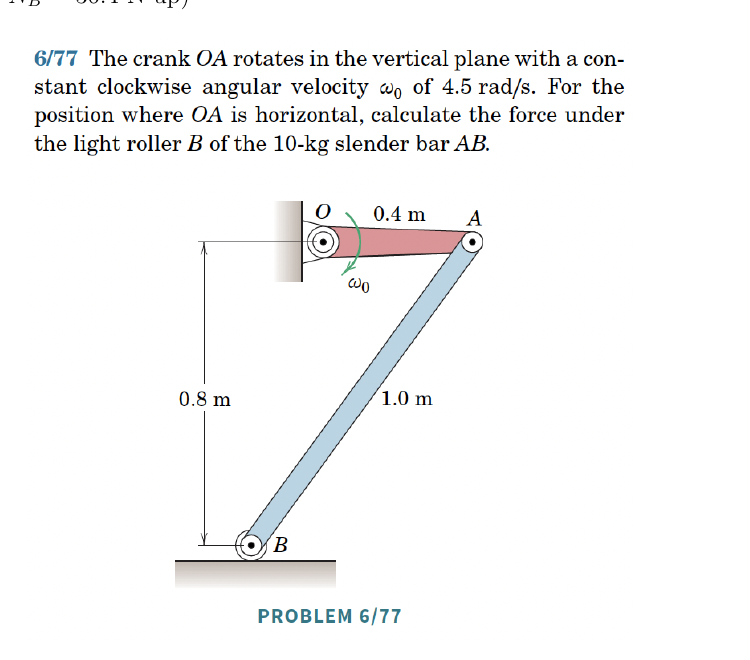
\includegraphics[width=0.5\linewidth,height=\textheight,keepaspectratio]{rigid_body_dynamics/../figures/rigid_body_kinetics/problems/06-077.png}

}

\caption{MKB 06-077.}

\end{figure}%

\subsection{Set 22 -- Impulse and Momentum for Rigid
Bodies}\label{set-22-impulse-and-momentum-for-rigid-bodies}

\textbf{1.} {[}MKB 06-136{]} \emph{(ans. \(\omega=1.811\) rad/s CCW)}

\begin{figure}[H]

{\centering 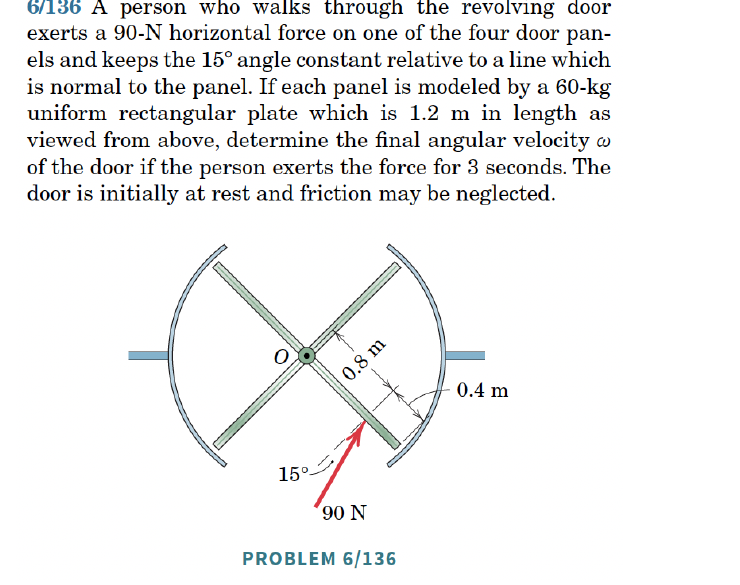
\includegraphics[width=0.5\linewidth,height=\textheight,keepaspectratio]{rigid_body_dynamics/../figures/rigid_body_kinetics/problems/06-136.png}

}

\caption{MKB 06-136.}

\end{figure}%

\textbf{2.} {[}MKB 06-142{]} \emph{(ans.
\(\mathbf{v}=\frac{Mu_M\mathbf{E}_x+m\mathbf{v}_m}{M+m}\),
\(\omega=\frac{12vm}{L(4M+7m)}\) CCW)}

\begin{figure}[H]

{\centering 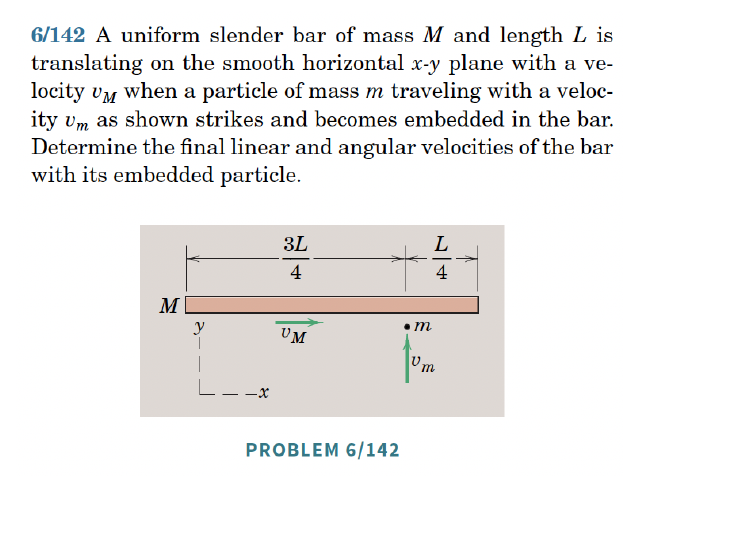
\includegraphics[width=0.5\linewidth,height=\textheight,keepaspectratio]{rigid_body_dynamics/../figures/rigid_body_kinetics/problems/06-142.png}

}

\caption{MKB 06-142.}

\end{figure}%

\textbf{3.} {[}06-145{]} \emph{(ans. \(\omega=\frac{3mv_1}{(M+m)L}\)
CW)}

\begin{figure}[H]

{\centering 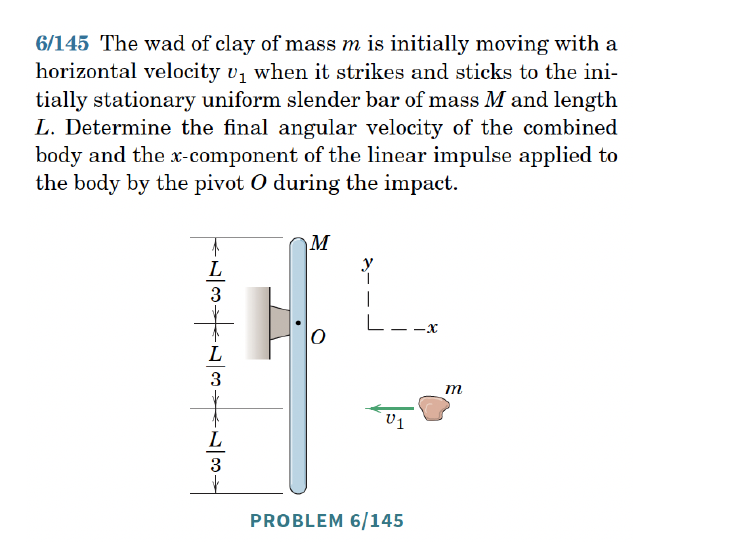
\includegraphics[width=0.5\linewidth,height=\textheight,keepaspectratio]{rigid_body_dynamics/../figures/rigid_body_kinetics/problems/06-145.png}

}

\caption{MKB 06-145.}

\end{figure}%

\textbf{4.} {[}06-146{]} \emph{(ans. \(N=2.04\) rev/s)}

\begin{figure}[H]

{\centering 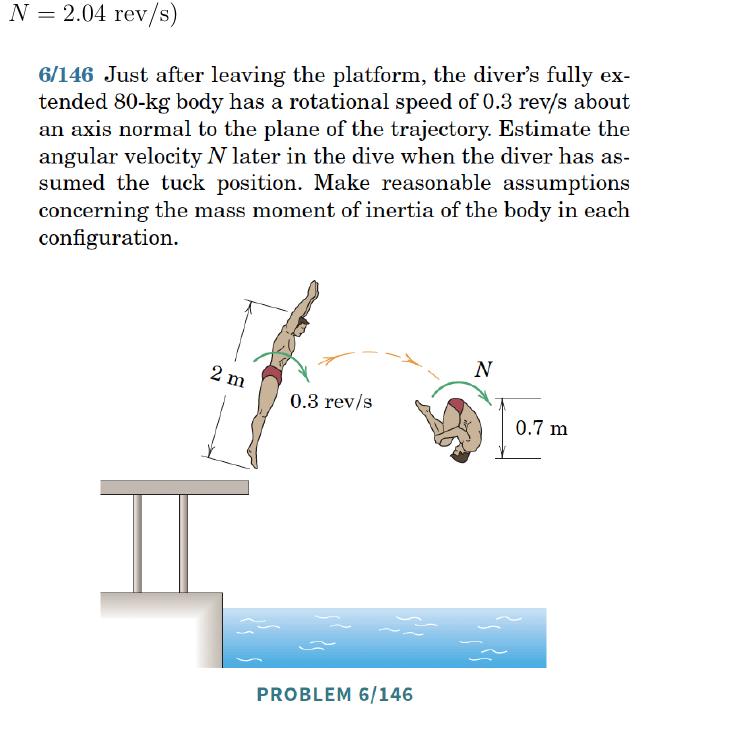
\includegraphics[width=0.5\linewidth,height=\textheight,keepaspectratio]{rigid_body_dynamics/../figures/rigid_body_kinetics/problems/06-146.png}

}

\caption{MKB 06-146.}

\end{figure}%

\textbf{5.} {[}06-148{]} \emph{(ans. \(\omega=1.593\) rad/s CCW,
\(n=91.7\%\))}

\begin{figure}[H]

{\centering 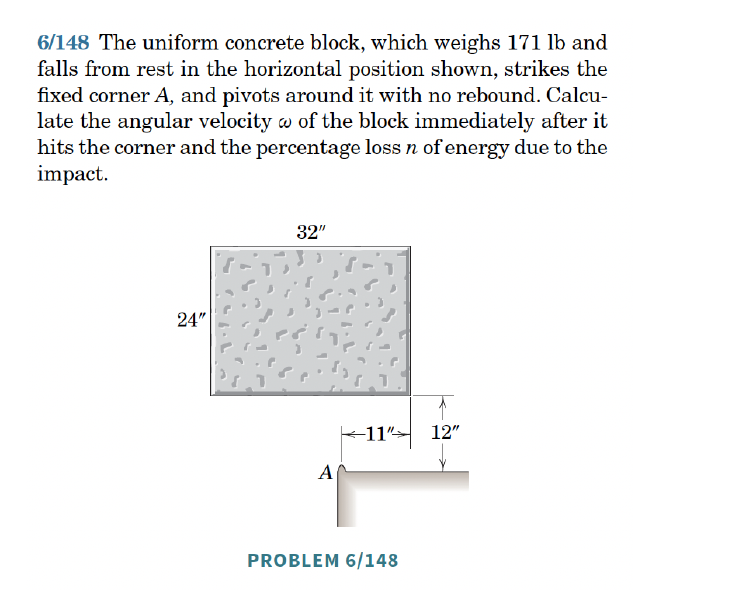
\includegraphics[width=0.5\linewidth,height=\textheight,keepaspectratio]{rigid_body_dynamics/../figures/rigid_body_kinetics/problems/06-148.png}

}

\caption{MKB 06-148.}

\end{figure}%

\textbf{6.} {[}06-155{]} \emph{(ans.
\(t=\frac{2v_0}{g(7\mu_k\cos\theta-2\sin\theta)}\))}

\begin{figure}[H]

{\centering \includegraphics[width=0.5\linewidth,height=\textheight,keepaspectratio]{rigid_body_dynamics/../figures/rigid_body_kinetics/problems/06-155.png}

}

\caption{MKB 06-155.}

\end{figure}%

\url{https://youtu.be/0N8tDgnrXNA}

\chapter{The Work-Energy Theorem for a Rigid
Body}\label{the-work-energy-theorem-for-a-rigid-body}

The \textbf{Koenig decomposition} for the kinetic energy of a rigid body
is: \begin{align}
    T = \frac{1}{2}m{\bf v}_C\cdot{\bf v}_C+\frac{1}{2}{\bf H}^C\cdot\bomega.
\end{align} In this class, \(\bomega = \omega{\bf E}_z\), so
\(\frac{1}{2}{\bf H}^C\cdot\bomega = \frac{1}{2}I_{zz}\omega^2\).

For fixed point rotation about \(O\), the kinetic energy simplifies to:
\begin{align}
    T = \frac{1}{2}{\bf H}^O\cdot\bomega
\end{align} which further simplifies to
\(T = \frac{1}{2}I^O_{zz}\omega^2\) if \(\bomega = \omega{\bf E}_z\).

The \textbf{work-energy theorem} for a rigid body has two equivalent
forms: \begin{align}
    \frac{dT}{dt} = {\bf F}\cdot{\bf v}_C+{\bf M}^C\cdot\bomega = \sum_{i=1}^N{\bf F}_i\cdot{\bf v}_i+{\bf M}_e\cdot\bomega.
\end{align} Integrating from \(t_A\) to \(t_B\): \begin{align}
    T_B-T_A = W_{{\bf F},AB}+W_{{\bf M},AB} = \sum_{i=1}^N W_{{\bf F}_i,AB}+W_{{\bf M}_e,AB},
\end{align} where \begin{align}
    W_{{\bf F},AB} &= \int_{t_A}^{t_B}{\bf F}\cdot{\bf v}_C\,dt, &
    W_{{\bf M},AB} &= \int_{t_A}^{t_B}{\bf M}^C\cdot\bomega\,dt,\\
    W_{{\bf F}_i,AB} &= \int_{t_A}^{t_B}{\bf F}_i\cdot{\bf v}_i\,dt, &
    W_{{\bf M}_e,AB} &= \int_{t_A}^{t_B}{\bf M}_e\cdot\bomega\,dt.
\end{align} Notice: the work of a force uses the velocity of its
\textbf{point of application}.

\url{https://youtu.be/acmYFwl8rRo}

\section{Koenig's Decomposition}\label{koenigs-decomposition}

By definition, the kinetic energy \(T\) of a rigid body is the
(continuous) sum of the kinetic energies of the differential masses
composing it: \begin{align}
    T = \frac{1}{2}\int_{\mathcal{B}}{\bf v}\cdot{\bf v}\,\rho\,dv.
\end{align} We can introduce the \({\bf v}_C\) term through
\begin{align}
    \begin{split}
        & {\bf v} = {\bf v}_C+\bomega\times\bpi,\\
        & \bpi = {\bf r}-{\bf r}_C,\\
        & \bomega = \omega_x{\bf e}_x+\omega_y{\bf e}_y+\omega_z{\bf e}_z.
    \end{split}
\end{align} Since \begin{align}
    {\bf v}\cdot{\bf v} = ({\bf v}_C+\bomega\times\bpi)\cdot({\bf v}_C+\bomega\times\bpi) = {\bf v}_C\cdot{\bf v}_C+{\bf v}_C\cdot(\bomega\times\bpi)+(\bomega\times\bpi)\cdot{\bf v}_C+(\bomega\times\bpi)\cdot(\bomega\times\bpi),
\end{align} and the two middle terms are equal by commutativity of the
dot product, substituting the above expressions in the kinetic energy
integral, we get \begin{align}
    T = \frac{1}{2}\int_{\mathcal{B}}\lp{\bf v}_C\cdot{\bf v}_C+2{\bf v}_C\cdot(\bomega\times\bpi)+(\bomega\times\bpi)\cdot(\bomega\times\bpi)\rp dm.
\end{align} For the first two terms in the above integral, \begin{align}
    \begin{split}
        & \frac{1}{2}\int_{\mathcal{B}}{\bf v}_C\cdot{\bf v}_C\,dm = \frac{{\bf v}_C\cdot{\bf v}_C}{2}\int dm = \frac{1}{2}m{\bf v}_C\cdot{\bf v}_C,\\
        & \int_{\mathcal{B}}{\bf v}_C\cdot(\bomega\times\bpi)\,dm = {\bf v}_C\cdot\lp\bomega\times\int\bpi\,dm\rp = 0.
    \end{split}
\end{align} Thus, \begin{align}
    T = \frac{1}{2}m{\bf v}_C\cdot{\bf v}_C+\frac{1}{2}\int_{\mathcal{B}}(\bomega\times\bpi)\cdot(\bomega\times\bpi)\,dm.
\end{align} We can simplify
\((\bomega\times\bpi)\cdot(\bomega\times\bpi)\) using the scalar triple
product identity
\(({\bf A}\times{\bf B})\cdot{\bf C}={\bf A}\cdot({\bf B}\times{\bf C})\)
with \({\bf A}=\bomega\), \({\bf B}=\bpi\),
\({\bf C}=\bomega\times\bpi\): \begin{align}
    (\bomega\times\bpi)\cdot(\bomega\times\bpi) = \bomega\cdot\lp\bpi\times(\bomega\times\bpi)\rp.
\end{align} The inner cross product expands via the BAC-CAB identity,
\({\bf a}\times({\bf b}\times{\bf c}) = {\bf b}({\bf a}\cdot{\bf c})-{\bf c}({\bf a}\cdot{\bf b})\),
with \({\bf a}=\bpi,{\bf b}=\bomega,{\bf c}=\bpi\): \begin{align}
    \bpi\times(\bomega\times\bpi) = (\bpi\cdot\bpi)\bomega-(\bpi\cdot\bomega)\bpi.
\end{align} Recall that \begin{align}
    {\bf H}^C = \int_{\mathcal{B}}\bpi\times(\bomega\times\bpi)\,dm = \int_{\mathcal{B}}\lp(\bpi\cdot\bpi)\bomega-(\bpi\cdot\bomega)\bpi\rp dm.
\end{align} Putting the last two results together, and pulling
\(\bomega\) out of the integral since it is the same for every material
point of the rigid body: \begin{align}
    \frac{1}{2}\int_{\mathcal{B}}(\bomega\times\bpi)\cdot(\bomega\times\bpi)\,dm = \frac{1}{2}\bomega\cdot\int_{\mathcal{B}}\bpi\times(\bomega\times\bpi)\,dm = \frac{1}{2}\bomega\cdot{\bf H}^C = \frac{1}{2}{\bf H}^C\cdot\bomega.
\end{align} Hence, we obtain the Koenig decomposition: \begin{align}
    T = \frac{1}{2}m{\bf v}_C\cdot{\bf v}_C+\frac{1}{2}{\bf H}^C\cdot\bomega.
\end{align}

\url{https://youtu.be/3HRYCW7wiRs}

\subsection{Fixed Point Rotation}\label{fixed-point-rotation}

In the case of fixed point rotation,
\({\bf v}_C = \bomega\times({\bf r}_C-{\bf r}_O)\) and
\({\bf v}_O = {\bf 0}\). Since \({\bf G}=m{\bf v}_C\) is the linear
momentum, \begin{align}
    \frac{1}{2}m{\bf v}_C\cdot{\bf v}_C = \frac{1}{2}(m{\bf v}_C)\cdot{\bf v}_C = \frac{1}{2}{\bf G}\cdot{\bf v}_C = \frac{1}{2}{\bf G}\cdot(\bomega\times{\bf r}_{C/O}),
\end{align} so, using the cyclical property of the scalar triple
product,
\({\bf a}\cdot({\bf b}\times{\bf c}) = {\bf b}\cdot({\bf c}\times{\bf a}) = {\bf c}\cdot({\bf a}\times{\bf b})\):
\begin{align}
    \begin{split}
        T &= \frac{1}{2}{\bf G}\cdot(\bomega\times{\bf r}_{C/O})+\frac{1}{2}{\bf H}^C\cdot\bomega\\
        &= \frac{1}{2}\bomega\cdot({\bf r}_{C/O}\times{\bf G})+\frac{1}{2}{\bf H}^C\cdot\bomega\\
        &= \frac{1}{2}({\bf r}_{C/O}\times{\bf G}+{\bf H}^C)\cdot\bomega\\
        &= \frac{1}{2}{\bf H}^O\cdot\bomega,
    \end{split}
\end{align} where the second line follows from the cyclical identity,
the third line factors \(\bomega\) out of the sum of two dot products,
and the last line uses the identity \begin{align}
    {\bf H}^O = {\bf H}^C+{\bf r}_{C/O}\times{\bf G},
\end{align} obtained by writing \begin{align}
    {\bf H}^O=\int_{\mathcal{B}}({\bf r}-{\bf r}_O)\times{\bf v}\,dm=\int_{\mathcal{B}}(\bpi+{\bf r}_{C/O})\times{\bf v}\,dm=\int_{\mathcal{B}}\bpi\times{\bf v}\,dm+{\bf r}_{C/O}\times\int_{\mathcal{B}}{\bf v}\,dm,
\end{align} and noting that
\(\int_{\mathcal{B}}\bpi\times{\bf v}\,dm={\bf H}^C\) (by the same steps
used above, since \(\int\bpi\,dm={\bf 0}\)) while
\(\int_{\mathcal{B}}{\bf v}\,dm=m{\bf v}_C={\bf G}\).

\url{https://youtu.be/3bu7kY8JLpM}

\section{Derivation of the Work-Energy
Theorem}\label{derivation-of-the-work-energy-theorem}

Taking the time derivative of
\(T = \frac{1}{2}m{\bf v}_C\cdot{\bf v}_C+\frac{1}{2}{\bf H}^C\cdot\bomega\):
\begin{align}
    \dot{T} = \frac{1}{2}m\dot{\bf v}_C\cdot{\bf v}_C+\frac{1}{2}m{\bf v}_C\cdot\dot{\bf v}_C+\frac{1}{2}\dot{\bf H}^C\cdot\bomega+\frac{1}{2}{\bf H}^C\cdot\dot{\bomega}.
\end{align} We need to show that
\(\dot{\bf H}^C\cdot\bomega = {\bf H}^C\cdot\dot{\bomega}\).
\begin{align}
    \begin{split}
        \balpha = \dot{\bomega} &= \frac{d}{dt}(\omega_x{\bf e}_x+\omega_y{\bf e}_y+\omega_z{\bf e}_z)\\
        &= \dot{\omega}_x{\bf e}_x+\dot{\omega}_y{\bf e}_y+\dot{\omega}_z{\bf e}_z+\omega_x\dot{\bf e}_x+\omega_y\dot{\bf e}_y+\omega_z\dot{\bf e}_z\\
        &= \dot{\omega}_x{\bf e}_x+\dot{\omega}_y{\bf e}_y+\dot{\omega}_z{\bf e}_z+\bomega\times(\omega_x{\bf e}_x+\omega_y{\bf e}_y+\omega_z{\bf e}_z)\\
        &= \dot{\omega}_x{\bf e}_x+\dot{\omega}_y{\bf e}_y+\dot{\omega}_z{\bf e}_z.
    \end{split}
\end{align} A direct calculation using this expression for \(\balpha\)
shows that \begin{align}
    {\bf H}^C\cdot\dot{\bomega} = (I_{xx}\omega_x+I_{xy}\omega_y+I_{xz}\omega_z)\dot{\omega}_x+(I_{xy}\omega_x+I_{yy}\omega_y+I_{yz}\omega_z)\dot{\omega}_y+(I_{xz}\omega_x+I_{yz}\omega_y+I_{zz}\omega_z)\dot{\omega}_z.
\end{align} To compute the corresponding expression for
\(\dot{\bf H}^C\cdot\bomega\), recall
\(\dot{\bf H}^C=\overset{\circ}{{\bf H}^C}+\bomega\times{\bf H}^C\), so
\begin{align}
    \dot{\bf H}^C\cdot\bomega = \overset{\circ}{{\bf H}^C}\cdot\bomega+(\bomega\times{\bf H}^C)\cdot\bomega = \overset{\circ}{{\bf H}^C}\cdot\bomega,
\end{align} since \((\bomega\times{\bf H}^C)\cdot\bomega=0\) (the vector
\(\bomega\times{\bf H}^C\) is perpendicular to \(\bomega\)). Using the
component expression for \(\overset{\circ}{{\bf H}^C}\) and dotting with
\(\bomega\): \begin{align}
    \overset{\circ}{{\bf H}^C}\cdot\bomega = (I_{xx}\dot{\omega}_x+I_{xy}\dot{\omega}_y+I_{xz}\dot{\omega}_z)\omega_x+(I_{xy}\dot{\omega}_x+I_{yy}\dot{\omega}_y+I_{yz}\dot{\omega}_z)\omega_y+(I_{xz}\dot{\omega}_x+I_{yz}\dot{\omega}_y+I_{zz}\dot{\omega}_z)\omega_z.
\end{align} Comparing this term by term with the expression for
\({\bf H}^C\cdot\dot{\bomega}\) above, and using the symmetry of the
inertia tensor (\(I_{xy}=I_{yx}\), \(I_{xz}=I_{zx}\),
\(I_{yz}=I_{zy}\)), every term matches
(e.g.~\(I_{xy}\dot{\omega}_x\omega_y = I_{xy}\omega_x\dot{\omega}_y\)).
Hence \(\dot{\bf H}^C\cdot\bomega = {\bf H}^C\cdot\dot{\bomega}\).
Consequently, \begin{align}
    \dot{T} = \frac{1}{2}m\dot{\bf v}_C\cdot{\bf v}_C+\frac{1}{2}m{\bf v}_C\cdot\dot{\bf v}_C+\frac{1}{2}\dot{\bf H}^C\cdot\bomega+\frac{1}{2}\dot{\bf H}^C\cdot\bomega,
\end{align} which implies that \begin{align}
    \dot{T} = m\dot{\bf v}_C\cdot{\bf v}_C+\dot{\bf H}^C\cdot\bomega.
\end{align} Invoking the balance of linear momentum and the balance of
angular momentum, we obtain the work-energy theorem: \begin{align}
    \dot{T} = {\bf F}\cdot{\bf v}_C+{\bf M}^C\cdot\bomega.
\end{align} This is a natural extension of the work-energy theorem for a
single particle.

\url{https://youtu.be/vCROTYHJRow}

\section{Alternative Form}\label{alternative-form}

Recall, \begin{align}
    \begin{split}
        & {\bf F} = \sum_{i=1}^K{\bf F}_i\\
        & {\bf M}^C = {\bf M}_e+\sum_{i=1}^K({\bf r}_i-{\bf r}_C)\times{\bf F}_i
    \end{split}
\end{align} Hence, the mechanical power of the resultant forces and
moments can be written as \begin{align}
    {\bf F}\cdot{\bf v}_C+{\bf M}^C\cdot\bomega = \lp\sum_{i=1}^K{\bf F}_i\rp\cdot{\bf v}_C+{\bf M}_e\cdot\bomega+\lp\sum_{i=1}^K({\bf r}_i-{\bf r}_C)\times{\bf F}_i\rp\cdot\bomega.
\end{align} With \({\bf a}=\bomega\), \({\bf b}={\bf r}_i-{\bf r}_C\),
\({\bf c}={\bf F}_i\), the identity
\({\bf a}\cdot({\bf b}\times{\bf c}) = {\bf c}\cdot({\bf a}\times{\bf b})\)
gives \begin{align}
    \lp({\bf r}_i-{\bf r}_C)\times{\bf F}_i\rp\cdot\bomega = \bomega\cdot\lp({\bf r}_i-{\bf r}_C)\times{\bf F}_i\rp = {\bf F}_i\cdot\lp\bomega\times({\bf r}_i-{\bf r}_C)\rp.
\end{align} Substituting this into the expression for
\({\bf F}\cdot{\bf v}_C+{\bf M}^C\cdot\bomega\) above: \begin{align}
    {\bf F}\cdot{\bf v}_C+{\bf M}^C\cdot\bomega = \sum_{i=1}^K{\bf F}_i\cdot{\bf v}_C+{\bf M}_e\cdot\bomega+\sum_{i=1}^K{\bf F}_i\cdot\lp\bomega\times({\bf r}_i-{\bf r}_C)\rp = \sum_{i=1}^K{\bf F}_i\cdot\lp{\bf v}_C+\bomega\times({\bf r}_i-{\bf r}_C)\rp+{\bf M}_e\cdot\bomega.
\end{align} Noting that
\({\bf v}_i = {\bf v}_C+\bomega\times({\bf r}_i-{\bf r}_C)\), we find
that \begin{align}
    {\bf F}\cdot{\bf v}_C+{\bf M}^C\cdot\bomega = \sum_{i=1}^K{\bf F}_i\cdot{\bf v}_i+{\bf M}_e\cdot\bomega.
\end{align} In conclusion, we have an alternative form of the
work-energy theorem that proves to be far easier to use in applications:
\begin{align}
    \dot{T} = \sum_{i=1}^K{\bf F}_i\cdot{\bf v}_i+{\bf M}_e\cdot\bomega.
\end{align} Each force is dotted with the velocity of its point of
application.

\section{Conservative Moments}\label{conservative-moments}

\subsection{Torsional Spring}\label{torsional-spring}

A torsional spring is just a model for some kind of elasticity at the
joint.

\begin{center}
\pandocbounded{\includegraphics[keepaspectratio]{rigid_body_dynamics/work_energy_theorem_files/figure-pdf/unnamed-chunk-1-1.pdf}}
\end{center}

A torsional spring with stiffness \(K\) creates a couple
\({\bf M}_S = -K\theta{\bf E}_z\). Its power is: \begin{align}
    {\bf M}_S\cdot\bomega = -K\theta\dot{\theta} = -\frac{d}{dt}\lp\frac{K\theta^2}{2}\rp.
\end{align} Hence \(U = \frac{1}{2}K\theta^2\) for the torsional spring.

\subsection{Constant Couple}\label{constant-couple}

A constant couple \({\bf M}_e = M_e{\bf E}_z\) has power
\({\bf M}_e\cdot\bomega = M_e\dot{\theta} = -\frac{d}{dt}(-M_e\theta)\).
Hence \(U = -M_e\theta\).

\begin{tcolorbox}[enhanced jigsaw, arc=.35mm, bottomrule=.15mm, bottomtitle=1mm, breakable, colback=white, colbacktitle=quarto-callout-important-color!10!white, colframe=quarto-callout-important-color-frame, coltitle=black, left=2mm, leftrule=.75mm, opacityback=0, opacitybacktitle=0.6, rightrule=.15mm, title=\textcolor{quarto-callout-important-color}{\faExclamation}\hspace{0.5em}{Note!}, titlerule=0mm, toprule=.15mm, toptitle=1mm]

These results apply only for \(\bomega = \omega{\bf E}_z\). Constant
couples are not conservative in general.

\end{tcolorbox}

\section{Examples}\label{examples}

\subsection{Bar Pendulum Fixed at Its
End}\label{bar-pendulum-fixed-at-its-end}

\begin{center}
\pandocbounded{\includegraphics[keepaspectratio]{rigid_body_dynamics/work_energy_theorem_files/figure-pdf/unnamed-chunk-2-1.pdf}}
\end{center}

A bar of length \(\ell\) and mass \(m\) pinned at its end. The energy is
conserved: \begin{align}
    U &= -\frac{mg\ell}{2}\cos\theta,\\
    E &= \frac{m\ell^2}{6}\dot{\theta}^2-\frac{mg\ell}{2}\cos\theta = \text{const}.
\end{align}

\subsection{Bar Pendulum With End
Mass}\label{bar-pendulum-with-end-mass}

\begin{center}
\pandocbounded{\includegraphics[keepaspectratio]{rigid_body_dynamics/work_energy_theorem_files/figure-pdf/unnamed-chunk-3-1.pdf}}
\end{center}

Adding a dead mass \(m_e\) at the end: \begin{align}
    U = -\frac{mg\ell}{2}\cos\theta-m_e g\ell\cos\theta.
\end{align}

\subsection{Follower Force}\label{follower-force}

What happens if there is a follower force applied at the end of the rod
always perpendicular to it?

\begin{center}
\pandocbounded{\includegraphics[keepaspectratio]{rigid_body_dynamics/work_energy_theorem_files/figure-pdf/unnamed-chunk-4-1.pdf}}
\end{center}

If instead a follower force \({\bf P}\) is applied perpendicular to the
bar at its end, this force is \textbf{nonconservative} (its direction
actively changes with configuration). Energy is not conserved.

\section{Energy Conservation}\label{energy-conservation}

As with particles and systems of particles, this theorem can be used to
establish conservation of the total mechanical energy of a rigid body,
\(E = T + U\), when all work-doing forces and moments are conservative.

\section{Summary}\label{summary-13}

\textbf{Koenig decomposition} of kinetic energy: \begin{align}
    T = \tfrac{1}{2}m\mathbf{v}_C\cdot\mathbf{v}_C + \tfrac{1}{2}\mathbf{H}^C\cdot\boldsymbol{\omega}.
\end{align} If a point \(O\) has zero velocity:
\(T = \tfrac{1}{2}\mathbf{H}^O\cdot\boldsymbol{\omega}\).

\textbf{Work--energy theorem for a rigid body}: \begin{align}
    \frac{dT}{dt} = \mathbf{F}\cdot\mathbf{v}_C + \mathbf{M}\cdot\boldsymbol{\omega} = \sum_i \mathbf{F}_i\cdot\mathbf{v}_i + M_e\omega.
\end{align}

\section{Exercises}\label{exercises-16}

\emph{The following problems are from Set 23 -- Work--Energy Theorem for
Rigid Bodies.}

\textbf{1.} {[}MKB 06-096{]} \emph{(ans. \(v_A=\sqrt{2gx\sin\theta}\),
\(v_B=\sqrt{gx\sin\theta}\))}

\begin{figure}[H]

{\centering \includegraphics[width=0.5\linewidth,height=\textheight,keepaspectratio]{rigid_body_dynamics/../figures/work_energy_theorem/06-096.png}

}

\caption{MKB 06-096.}

\end{figure}%

\textbf{2.} {[}MKB 06-099{]} \emph{(ans.
\(\omega_{\max}=0.861\sqrt{g/b}\))}

\begin{figure}[H]

{\centering \includegraphics[width=0.5\linewidth,height=\textheight,keepaspectratio]{rigid_body_dynamics/../figures/work_energy_theorem/06-099.png}

}

\caption{MKB 06-099.}

\end{figure}%

\textbf{3.} {[}06-108{]} \emph{(ans. (a) \(k=93.3\) N/m; (b)
\(\omega=1.484\) rad/s CW)}

\begin{figure}[H]

{\centering \includegraphics[width=0.5\linewidth,height=\textheight,keepaspectratio]{rigid_body_dynamics/../figures/work_energy_theorem/06-108.png}

}

\caption{06-108.}

\end{figure}%

\textbf{4.} {[}06-112{]} \emph{(ans. \(x=0.211l\),
\(\omega_{\max}=1.861\sqrt{g/l}\) CW)}

\begin{figure}[H]

{\centering \includegraphics[width=0.5\linewidth,height=\textheight,keepaspectratio]{rigid_body_dynamics/../figures/work_energy_theorem/06-112.png}

}

\caption{06-112.}

\end{figure}%

\textbf{5.} {[}06-118{]} \emph{(ans.
\(v_A=\sqrt{3}\sqrt{\frac{M\theta}{m}-gb(1-\cos\theta)}\) right)}

\begin{figure}[H]

{\centering \includegraphics[width=0.5\linewidth,height=\textheight,keepaspectratio]{rigid_body_dynamics/../figures/work_energy_theorem/06-118.png}

}

\caption{06-118.}

\end{figure}%

\url{https://youtu.be/-jdslhyHAIY}

\chapter{Systems of Particles and Rigid
Bodies}\label{systems-of-particles-and-rigid-bodies}

The balance laws developed separately for particles, systems of
particles, and rigid bodies apply just as well to \emph{combinations} of
these --- assemblies of rigid bodies and particles connected by pins,
rods, or motors. The following example illustrates how to set up such a
problem: identifying the kinematic constraints between the bodies,
drawing free-body diagrams of the combined system and of its parts, and
applying the balance laws to each.

\section{Example: BB8}\label{example-bb8}

Consider a spherical robot composed of a spherical shell of mass \(m\)
and radius \(R\) and a bar of mass \(2m\) and length \(\ell<2R\) pinned
at point \(A\), its center, to the center of the shell as shown in the
figure below. A geared motor drive at \(A\) provides an internal moment
which rotates the bar. The friction between the robot and the ground is
sufficient to prevent slipping.

Throughout the motion, the position vector from the origin to the center
of the robot is \({\bf r}_A = x{\bf E}_x+R{\bf E}_y\).

The angular velocity of the spherical shell is
\(\bomega_1 = \dot{\theta}_1{\bf E}_z\) and the angular velocity of the
bar of length \(\ell\) is \(\bomega_2 = \dot{\theta}_2{\bf E}_z\).

\begin{center}
\pandocbounded{\includegraphics[keepaspectratio]{rigid_body_dynamics/systems_of_particles_and_rigid_bodies_files/figure-pdf/unnamed-chunk-1-1.pdf}}
\end{center}

\begin{enumerate}
\def\labelenumi{(\alph{enumi})}
\item
  Draw the free-body diagram of (1) the combined system of the spherical
  shell and the bar of length \(\ell\), (2) the spherical shell with its
  massless diameter alone, and (3) the bar of length \(\ell\) alone.
\item
  We wish to determine the motion of the robot, i.e., we want to find
  \(x(t)\), \(\theta_1(t)\), \(\theta_2(t)\), resulting from the moments
  applied by the motor. How do we proceed?
\end{enumerate}

\subsection{Free-Body Diagrams}\label{free-body-diagrams-1}

\textbf{Combined system} (shell + bar):

\begin{center}
\pandocbounded{\includegraphics[keepaspectratio]{rigid_body_dynamics/systems_of_particles_and_rigid_bodies_files/figure-pdf/unnamed-chunk-2-1.pdf}}
\end{center}

\textbf{Spherical shell alone:}

\begin{center}
\pandocbounded{\includegraphics[keepaspectratio]{rigid_body_dynamics/systems_of_particles_and_rigid_bodies_files/figure-pdf/unnamed-chunk-3-1.pdf}}
\end{center}

\textbf{Bar alone:}

\begin{center}
\pandocbounded{\includegraphics[keepaspectratio]{rigid_body_dynamics/systems_of_particles_and_rigid_bodies_files/figure-pdf/unnamed-chunk-4-1.pdf}}
\end{center}

where \begin{align}
    {\bf F}_f = F_f{\bf E}_x.
\end{align}

\subsection{Kinematics}\label{kinematics-2}

By differentiating \({\bf r}_A\), we get \begin{align}
    \begin{split}
        {\bf v}_A &= \dot{x}{\bf E}_x,\\
        {\bf a}_A &= \ddot{x}{\bf E}_x.
    \end{split}
\end{align}

The roll-without-slip condition between the sphere and the ground,
\({\bf v}_P={\bf 0}\), yields a relationship between \(x\) and
\(\theta_1\): \begin{align}
    \begin{split}
        {\bf v}_C &= \bomega_1\times R{\bf E}_y,\\
        \dot{x} &= -R\dot{\theta}_1.
    \end{split}
\end{align}

\subsection{Balance of Linear Momentum (Combined
System)}\label{balance-of-linear-momentum-combined-system}

\begin{align}
    {\bf F} = (m_1+m_2){\bf a}_A.
\end{align}

\begin{tcolorbox}[enhanced jigsaw, arc=.35mm, bottomrule=.15mm, bottomtitle=1mm, breakable, colback=white, colbacktitle=quarto-callout-note-color!10!white, colframe=quarto-callout-note-color-frame, coltitle=black, left=2mm, leftrule=.75mm, opacityback=0, opacitybacktitle=0.6, rightrule=.15mm, title=\textcolor{quarto-callout-note-color}{\faInfo}\hspace{0.5em}{Note}, titlerule=0mm, toprule=.15mm, toptitle=1mm]

This example is left as a set-up exercise: complete the balance of
linear momentum in components, then use the balance of angular momentum
(about \(A\) or about \(P\)) for the combined system, the shell alone,
and the bar alone, together with the kinematic constraint above, to
solve for \(x(t)\), \(\theta_1(t)\), \(\theta_2(t)\).

\end{tcolorbox}

\part{Lagrangian Mechanics}

\chapter{Lagrange's Equations of Motion for a System of
Particles}\label{lagranges-equations-of-motion-for-a-system-of-particles}

\section{Constraints}\label{constraints}

Put in simple terms, a holonomic constraint is a constraint which can be
written in terms of position coordinates, e.g.~\(x=0\). A nonholonomic
constraint is one which cannot be written in terms of position
coordinates, e.g.~\({\bf v}\cdot{\bf e}_\theta = 0\).

\begin{tcolorbox}[enhanced jigsaw, arc=.35mm, bottomrule=.15mm, bottomtitle=1mm, breakable, colback=white, colbacktitle=quarto-callout-tip-color!10!white, colframe=quarto-callout-tip-color-frame, coltitle=black, left=2mm, leftrule=.75mm, opacityback=0, opacitybacktitle=0.6, rightrule=.15mm, title=\textcolor{quarto-callout-tip-color}{\faLightbulb}\hspace{0.5em}{Think!}, titlerule=0mm, toprule=.15mm, toptitle=1mm]

Question: Consider a particle constrained to move on a horizontal
surface \(z=0\). Is this constraint holonomic?

\begin{quote}
\textbf{Answer}

\ldots{}
\end{quote}

\end{tcolorbox}

\begin{tcolorbox}[enhanced jigsaw, arc=.35mm, bottomrule=.15mm, bottomtitle=1mm, breakable, colback=white, colbacktitle=quarto-callout-tip-color!10!white, colframe=quarto-callout-tip-color-frame, coltitle=black, left=2mm, leftrule=.75mm, opacityback=0, opacitybacktitle=0.6, rightrule=.15mm, title=\textcolor{quarto-callout-tip-color}{\faLightbulb}\hspace{0.5em}{Think!}, titlerule=0mm, toprule=.15mm, toptitle=1mm]

Question: Consider two particles connected by a rigid massless rod of
length \(\ell\). What constraint is this system of two particles subject
to? Is this constraint holonomic or nonholonomic?

\begin{quote}
\textbf{Answer}

\ldots{}
\end{quote}

\end{tcolorbox}

\begin{tcolorbox}[enhanced jigsaw, arc=.35mm, bottomrule=.15mm, bottomtitle=1mm, breakable, colback=white, colbacktitle=quarto-callout-tip-color!10!white, colframe=quarto-callout-tip-color-frame, coltitle=black, left=2mm, leftrule=.75mm, opacityback=0, opacitybacktitle=0.6, rightrule=.15mm, title=\textcolor{quarto-callout-tip-color}{\faLightbulb}\hspace{0.5em}{Think!}, titlerule=0mm, toprule=.15mm, toptitle=1mm]

Question: Consider the system in the previous question where \(m_2\) is
subject to a knife-edge constraint \({\bf v}_2\cdot{\bf e}_2=0\). Is
this constraint holonomic or nonholonomic.

\pandocbounded{\includegraphics[keepaspectratio]{lagrangian_mechanics/lagranges_equations_files/figure-pdf/unnamed-chunk-1-1.pdf}}

\begin{quote}
\textbf{Answer}

\ldots{}
\end{quote}

\end{tcolorbox}

Frobenius' integrability criteria may be used to determine definitely if
a constraint or a system of constraints is holonomic or not. The
criterion is beyond the scope of the class. Here, we restrict our
attention to holonomic constraints.

\section{Lagrange's Prescription on
Constraints}\label{lagranges-prescription-on-constraints}

Consider a constraint of the form \begin{align*}
    {\bf f}_1\cdot{\bf v}_1+\hdots+{\bf f}_N\cdot{\bf v}_N + e = 0,
\end{align*} then the associated Lagrange prescription of the constraint
force is \(\mu{\bf f}_K\) applied at particle \(K\), \(K=1,\hdots,n\).

\begin{tcolorbox}[enhanced jigsaw, arc=.35mm, bottomrule=.15mm, bottomtitle=1mm, breakable, colback=white, colbacktitle=quarto-callout-tip-color!10!white, colframe=quarto-callout-tip-color-frame, coltitle=black, left=2mm, leftrule=.75mm, opacityback=0, opacitybacktitle=0.6, rightrule=.15mm, title=\textcolor{quarto-callout-tip-color}{\faLightbulb}\hspace{0.5em}{Think!}, titlerule=0mm, toprule=.15mm, toptitle=1mm]

Question: Prescribe the constraint force for a particle constrained on a
plane \(z = 0\).

\begin{quote}
\textbf{Answer}

This constraint may be written as \({\bf v}\cdot{\bf E}_z = 0\) and the
constraint force acting on the particle is \({\bf F} = \mu{\bf E}_z.\)
\end{quote}

\end{tcolorbox}

\begin{tcolorbox}[enhanced jigsaw, arc=.35mm, bottomrule=.15mm, bottomtitle=1mm, breakable, colback=white, colbacktitle=quarto-callout-tip-color!10!white, colframe=quarto-callout-tip-color-frame, coltitle=black, left=2mm, leftrule=.75mm, opacityback=0, opacitybacktitle=0.6, rightrule=.15mm, title=\textcolor{quarto-callout-tip-color}{\faLightbulb}\hspace{0.5em}{Think!}, titlerule=0mm, toprule=.15mm, toptitle=1mm]

Question: Prescribe the constraint force acting on a simple pendulum
associated with the constraint that the length of the pendulum is
constant.

\begin{quote}
\textbf{Answer}

A simple pendulum has the constraint \({\bf r} = 0\) which may be
written as \({\bf v}\cdot{\bf e}_r = 0\), then the constraint force
acting on the particle is \({\bf F} = \mu{\bf e}_r\).
\end{quote}

\end{tcolorbox}

\section{Unconstrained Equations}\label{unconstrained-equations}

Consider a system of \(n\) particles with \(3n\) coordinates. The system
is subject to \(m\) holonomic constraints, so the number of degrees of
freedom of the system is \(3n-m\). The generalized coordinates of the
system may be listed as \begin{align}
    q =
    \begin{bmatrix}
        x^1 & y^1 & z^1 & \cdots & x^n & y^n & z^n
    \end{bmatrix}^T
\end{align} and the corresponding generalized velocities are
\begin{align}
    u =
    \begin{bmatrix}
        v^{x1} & v^{y1} & v^{z1} & \cdots & v^{xn} & v^{yn} & v^{zn}
    \end{bmatrix}^T
\end{align} We define \(u\) so that later we set \(u = \dot{q}\).

We arrange the generalized coordinates such that the first \(3n-m\)
coordinates are the unconstrained degrees of freedom and the last \(m\)
coordinates are equal to the holonomic constraints, and can be later set
to zero.

\begin{tcolorbox}[enhanced jigsaw, arc=.35mm, bottomrule=.15mm, bottomtitle=1mm, breakable, colback=white, colbacktitle=quarto-callout-tip-color!10!white, colframe=quarto-callout-tip-color-frame, coltitle=black, left=2mm, leftrule=.75mm, opacityback=0, opacitybacktitle=0.6, rightrule=.15mm, title=\textcolor{quarto-callout-tip-color}{\faLightbulb}\hspace{0.5em}{Think!}, titlerule=0mm, toprule=.15mm, toptitle=1mm]

Question: Generalized coordinates for simple harmonic oscillator.

\begin{quote}
\textbf{Answer}

\(q = [x\ y\ z]\), \(u = [v_x\ v_y\ v_z]\).
\end{quote}

\end{tcolorbox}

\begin{tcolorbox}[enhanced jigsaw, arc=.35mm, bottomrule=.15mm, bottomtitle=1mm, breakable, colback=white, colbacktitle=quarto-callout-tip-color!10!white, colframe=quarto-callout-tip-color-frame, coltitle=black, left=2mm, leftrule=.75mm, opacityback=0, opacitybacktitle=0.6, rightrule=.15mm, title=\textcolor{quarto-callout-tip-color}{\faLightbulb}\hspace{0.5em}{Think!}, titlerule=0mm, toprule=.15mm, toptitle=1mm]

Question: Generalized coordinates for simple pendulum.

\begin{quote}
\textbf{Answer}

\(q = [\theta\ \beta\ z]\), \(u = [u_\theta\ u_\beta\ u_z]\) where
\(\beta = r-\ell\).
\end{quote}

\end{tcolorbox}

The kinetic energy of the system is \(T\), then Lagrange's equations of
motion of the system are \begin{align}
    \frac{d}{dt}\lp\frac{\partial T}{\partial u^i}\rp-\frac{\partial T}{\partial q^i} = \sum_{K=1}^n{\bf F}^K\cdot \frac{\partial {\bf r}^K}{\partial q^i}
\end{align} Equivalently, using the Lagrangian \(L = T-U\), where \(U\)
is the potential energy, the equations of motion of the system may be
written as \begin{align}
    \frac{d}{dt}\lp\frac{\partial L}{\partial u^i}\rp-\frac{\partial L}{\partial q^i} = \sum_{K=1}^n{\bf F}_{nonc}^K\cdot \frac{\partial {\bf r}^K}{\partial q^i}
\end{align} where \({\bf F}^K\) is the sum of external forces acting on
particle \(K\) while \({\bf F}_{nonc}^K\) is the sum of nonconservative
forces acting on \(K\).

\subsection{Advantage of Lagrange's
Equations}\label{advantage-of-lagranges-equations}

If the system is subject to \(m\) holonomic constraints, if you choose
the last \(m\) generalized coordinates to be equal to the constraints,
then the first \(m-n\) Lagrange's equations of motion will be uncoupled
from the holonomic constraint forces, these are the equations of motion.
The last \(n-m\) equations can be solved for the holonomic constraint
forces. If one does not wish to solve for these forces, one can just use
the constrained kinetic energy.

\section{Constrained Equations}\label{constrained-equations}

Consider a system of \(n\) particles with \(3n\) degrees of freedom and
\(m\) holonomic constraints prescribed using Lagrange's equations of
motion. The unconstrained degrees of freedom of the system are arranged
in an array of generalized coordinates \(q\) and generalized velocities
\(u\), and the constrained kinetic energy of the system is
\(\tilde{T}\), then Lagrange's equations of motion of the system are
\begin{align}
    \frac{d}{dt}\lp\frac{\partial \tilde{T}}{\partial u^i}\rp-\frac{\partial \tilde{T}}{\partial q^i} = \sum_{K=1}^n{\bf F}^K\cdot \frac{\partial {\bf r}^K}{\partial q^i}
\end{align} Equivalently, using the constrained Lagrangian
\(\tilde{L} = \tilde{T}-\tilde{U}\), where \(\tilde{U}\) is the
constrained potential energy, the equations of motion of the system may
be written as \begin{align}
    \frac{d}{dt}\lp\frac{\partial \tilde{L}}{\partial u^i}\rp-\frac{\partial \tilde{L}}{\partial q^i} = \sum_{K=1}^n{\bf F}_{nonc}^K\cdot \frac{\partial {\bf r}^K}{\partial q^i}
\end{align} If the forces are prescribed with Lagrange's prescription,
then \$
\sum\_\{K=1\}\^{}n\{\bf F\}\^{}K\cdot \frac{\partial {\bf r}^K}{\partial q^i}\$
and
\(\sum_{K=1}^n{\bf F}_{nonc}^K\cdot \frac{\partial {\bf r}^K}{\partial q^i}\)
reduce to
\(\sum_{K=1}^n{\bf F}_{appliedc}\cdot\frac{\partial {\bf r}^K}{\partial q^i}\)
and
\(\sum_{K=1}^n{\bf F}_{applied, nconc}\cdot\frac{\partial {\bf r}^K}{\partial q^i}\)
respectively, that is the applied forces and the nonconservative applied
forces.

In many cases, the nonconservative applied forces are zero, hence the
commonly known homogeneous form of Lagrange's equation \begin{align}
    \frac{d}{dt}\lp\frac{\partial \tilde{L}}{\partial u^i}\rp-\frac{\partial \tilde{L}}{\partial q^i} = 0.
\end{align}

\section{Example: Simple Harmonic
Oscillator}\label{example-simple-harmonic-oscillator}

Consider a simple harmonic oscillator of mass \(m\) connected to a
linear spring of unstretched length \(\ell_0\) and stiffness \(k\). The
origin is taken at the location of \(m\) when the spring is unstretched
so that the position vector of \(m\) is \({\bf r} = x{\bf E}_x\) and
\(x\) denotes the stretch of the spring. The velocity of \(m\) is
\({\bf v} = v{\bf E}_x\). Find the equation of motion of the mass \(m\).

Using unconstrained Lagrangian: \begin{align}
    \begin{split}
        & q^1 = x,\qquad q^2 = y, \qquad q^3 = z,\\
        & u^1 = v_x,\qquad u^2 = v_y, \qquad u^3 = v_z,\\
    \end{split}
\end{align} Lagrangian \begin{align}
    L = T-U  = \frac{m}{2}\lp v_x^2+v_y^2+v_z^2\rp-mgz
\end{align} Constraint forces \(\mu_1{\bf E}_y\), \(\mu_2{\bf E}_z\).

Equation along \(z\), \begin{align}
    \begin{split}
        \dot{\bf v}_z+mg = \mu_2.
    \end{split}
\end{align}

Using constrained Lagrangian:

The kinetic energy of the spring is \(\tilde{T} = \frac{1}{2}v^2\) and
potential energy is \(\tilde{U} = \frac{1}{2}kx^2\), thus the Lagrangian
is \(\tilde{L} = \frac{1}{2}v^2-\frac{1}{2}kx^2\). Here, \(m\) has one
degree of freedom, so \(q = [x]\) and \(u = [v]\), so the equation of
motion of the system is obtained \ldots{}

\section{Example: Simple Pendulum}\label{example-simple-pendulum}

\begin{align}
    \begin{split}
        {\bf r} &= \ell{\bf e}_x,\\
        {\bf v} &= \ell\dot{\theta}{\bf e}_y
    \end{split}
\end{align} Gravitational potential energy

\section{Example: Double Pendulum}\label{example-double-pendulum}

\begin{align}
    \begin{split}
        {\bf r}_1 &= \ell_1\,{}_{1}{\bf e}_x,\\
        {\bf v}_1 &= \ell_1\dot{\theta}_1\,{}_{1}{\bf e}_y,\\
        {\bf r}_2 &= {\bf r}_1+\ell_2\,{}_{2}{\bf e}_x,\\
        {\bf v}_2 &= {\bf v}_1+\ell_2\dot{\theta}_2\,{}_{2}{\bf e}_y
    \end{split}
\end{align} Gravitational potential energy

\section{Alternative Principles of
Dynamics}\label{alternative-principles-of-dynamics}

Source: O'Reilly's textbook on Intermediate Dynamics, second edition,
Section 4.12

\begin{itemize}
\tightlist
\item
  Jean Bernoulli's principle of virtual work (1717) - for statics
\item
  D'Alembert's principle (1743) - extension of the principle of virtual
  work for dynamics
\item
  Gauss' principle of least constraint (1829)
\item
  Hamilton's principle (1835)
\end{itemize}

\subsection{Principle of Virtual Work and D'Alembert's
Principle}\label{principle-of-virtual-work-and-dalemberts-principle}

Consider the principle of virtual work and D'Alembert's Principle
applied to a system of particles. We assume that the particles are
subject to a single constraint: \begin{align*}
    {\bf f}_1\cdot{\bf v}_1+\hdots+{\bf f}_N\cdot{\bf v}_N + e = 0.
\end{align*} The principle of virtual work and D'Alembert's principle
collectively state that the motion of the system of particles is such
that the following equation is satisfied: \begin{align}
    \begin{split}
        \lp {\bf F}_{a1}-m_1\ddot{\bf r}_1\rp\cdot{\bf d}_1+\hdots+\lp {\bf F}_{aN}-m_N\ddot{\bf r}_N\rp\cdot{\bf d}_N = 0,
    \end{split}
\end{align} for all possible choices of the vectors
\({\bf d}_1, \hdots, {\bf d}_N\) that satisfy the condition
\begin{align}
    \begin{split}
        {\bf f}_1\cdot{\bf d}_1+\hdots+{\bf f}_N\cdot{\bf d}_N = 0.
    \end{split}
\end{align} The vectors \({\bf d}_K\) are known as the virtual
displacements and are usually denoted by \(\delta {\bf r}_K\). The
virtual work performed by the applied force \({\bf F}_{ak}\) is defined
as \({\bf F}_{ak}\cdot{\bf d}_K\); thus the equation above states that
the combined virtual work of the applied forces \({\bf F}_{aK}\) and the
inertial forces \(-m_K\ddot{\bf r}_K\) is zero.

How to obtain the equations of motion of the system of particles from
the equation above?

Introduce a Lagrange multiplier, which we denote by the scalar function
\(\mu = \mu(t)\), to accommodate the single constraint on the vectors
\({\bf d}_K\): \begin{align}
    \begin{split}
        \sum_{K=1}^N\lp{\bf F}_{aK}-m\ddot{\bf r}_N\rp\cdot{\bf d}_K+\mu\sum_{K=1}^N{\bf f}_K\cdot{\bf d}_K = 0.
    \end{split}
\end{align} As a consequence of the Lagrange multiplier \(\mu\), the
vectors \({\bf d}_K\) can be varied independently. For the previous
equation to hold for all such displacements, it is necessary and
sufficient that \begin{align}
    \begin{split}
        m_K\ddot{\bf r}_K = {\bf F}_{aK}+\mu{\bf f}_K \qquad (K=1,\hdots,N).
    \end{split}
\end{align} These equations are none other than the balances of linear
momenta for a system of particles subject to the above constraint, for
which the constraint forces are prescribed by use of Lagrange's
prescription: \begin{align}
    \begin{split}
        {\bf F}_{cK} = \mu{\bf f}_K\qquad (K=1,\dots,N).
    \end{split}
\end{align}

\subsection{Gauss' Principle of Least
Action}\label{gauss-principle-of-least-action}

Suppose we have a system of \(N\) particles that are subject to the
constraint \begin{align*}
    {\bf f}_1\cdot{\bf v}_1+\hdots+{\bf f}_N\cdot{\bf v}_N + e = 0.
\end{align*} and suppose that the constraint forces are prescribed by
using Lagrange's prescription \({\bf F}_{cK} = \mu{\bf f}_K\),
\((K=1,\hdots,N)\). Then, in any motion of the system that satisfies the
constraint, the constraint forces \({\bf F}_{cK} = \mu{\bf f}_K\) are
the least needed to ensure that the constraint is satisfied. That is,
Lagrange's prescription is in a sense optimal!

\subsection{Hamilton's Principle}\label{hamiltons-principle}

For ease of exposition, we restrict our discussion to a single particle
of mass \(m\) and suppose that the coordinates \(q = (q^1,q^2,q^2)\) are
used to parametrize the position vector. Hamilton's principle states
that the motion of the system between a given initial configuration
\(q(t_0)\) and a given final configuration \(q(t_1)\) is such that it
extremizes the integral: \begin{align}
    \begin{split}
        I = \int_{t_0}^{t_1}Ldt
    \end{split}
\end{align} where the Lagrangian \(L = T(q^i,u^i)-U(q^i)\) and \(t_0\)
and \(t_1\) are fixed instances of time.

There are an infinite number of paths \(q(t)\) that can connect two
possible configurations, and so finding one that extremizes \(I\)
appears to be a daunting task.

The necessary conditions for the components of \(q(t)\) to extremize
\(I\) are that \(q(t)\) satisfy the following differential equations:
\begin{align}
    \frac{d}{dt}\lp\frac{\partial L}{\partial u^i}\rp-\frac{\partial L}{\partial q^i} = 0\qquad (k = 1,2,3).
\end{align} In the context of extremizing \(I\) (calculus of
variations), these are known as the Euler-Lagrange equations.

\begin{center}
\pandocbounded{\includegraphics[keepaspectratio]{lagrangian_mechanics/lagranges_equations_files/figure-pdf/unnamed-chunk-2-1.pdf}}
\end{center}

\section{Exercises}\label{exercises-17}

Double pendulum

\begin{center}
\pandocbounded{\includegraphics[keepaspectratio]{lagrangian_mechanics/lagranges_equations_files/figure-pdf/unnamed-chunk-3-1.pdf}}
\end{center}

\bookmarksetup{startatroot}

\chapter*{References}\label{references}
\addcontentsline{toc}{chapter}{References}

\markboth{References}{References}

\protect\phantomsection\label{refs}
\begin{CSLReferences}{1}{1}
\bibitem[\citeproctext]{ref-lubliner2017introduction}
Lubliner, Jacob, and Panayiotis Papadopoulos. 2017. \emph{Introduction
to Solid Mechanics: An Integrated Approach}. Springer.
\url{https://doi.org/10.1007/978-1-4614-6768-7}.

\end{CSLReferences}

\part{Appendices}

\chapter{Mathematical Background for Conservative
Forces}\label{mathematical-background-for-conservative-forces}

\section{Gradient}\label{gradient}

In coordinate-free terms, the gradient of a function \(f({\bf r})\) is
defined by \begin{align}
    df = \nabla f\cdot d{\bf r},
\end{align} where \(df\) is the total infinitesimal change in \(f\) for
an infinitesimal displacement \(d{\bf r}\).

\subsection{Cartesian Coordinates}\label{cartesian-coordinates-1}

For \(f = f(x,y,z)\) with
\(d{\bf r} = dx{\bf E}_x+dy{\bf E}_y+dz{\bf E}_z\): \begin{align}
    df = \frac{\partial f}{\partial x}dx+\frac{\partial f}{\partial y}dy+\frac{\partial f}{\partial z}dz.
\end{align} Since this must hold for all independent variations \(dx\),
\(dy\), \(dz\): \begin{align}
    \nabla f = \frac{\partial f}{\partial x}{\bf E}_x+\frac{\partial f}{\partial y}{\bf E}_y+\frac{\partial f}{\partial z}{\bf E}_z.
\end{align}

\subsection{Cylindrical-Polar
Coordinates}\label{cylindrical-polar-coordinates-1}

For \(f = f(r,\theta,z)\) with
\(d{\bf r} = dr{\bf e}_r+r\,d\theta{\bf e}_\theta+dz{\bf E}_z\):
\begin{align}
    df = \frac{\partial f}{\partial r}dr+\frac{\partial f}{\partial \theta}d\theta+\frac{\partial f}{\partial z}dz = \nabla f\cdot(dr{\bf e}_r+r\,d\theta{\bf e}_\theta+dz{\bf E}_z).
\end{align} Matching coefficients: \begin{align}
    \nabla f = \frac{\partial f}{\partial r}{\bf e}_r+\frac{1}{r}\frac{\partial f}{\partial \theta}{\bf e}_\theta+\frac{\partial f}{\partial z}{\bf E}_z.
\end{align}

\subsection{Curvilinear Coordinates}\label{curvilinear-coordinates}

\begin{tcolorbox}[enhanced jigsaw, arc=.35mm, bottomrule=.15mm, bottomtitle=1mm, breakable, colback=white, colbacktitle=quarto-callout-note-color!10!white, colframe=quarto-callout-note-color-frame, coltitle=black, left=2mm, leftrule=.75mm, opacityback=0, opacitybacktitle=0.6, rightrule=.15mm, title=\textcolor{quarto-callout-note-color}{\faInfo}\hspace{0.5em}{Note}, titlerule=0mm, toprule=.15mm, toptitle=1mm]

This section is beyond the scope of this course. See O. M. O'Reilly's
\emph{Intermediate Dynamics} Section 1.6 for more information.

\end{tcolorbox}

Consider a curvilinear coordinate system \(\{q^1,q^2,q^3\}\) defined by
\(q^i = \hat{q}^i(x_1,x_2,x_3)\), assumed locally invertible. The
\textbf{covariant basis vectors} are: \begin{align}
    {\bf a}_i = \frac{\partial{\bf r}}{\partial q^i} = \sum_{k=1}^3\frac{\partial\hat{x}^k}{\partial q^i}{\bf E}_k.
\end{align} The \textbf{contravariant basis vectors} are the gradients
of the curvilinear coordinates: \begin{align}
    {\bf a}^k = \nabla q^k = \sum_{i=1}^3\frac{\partial\hat{q}^k}{\partial x_i}{\bf E}_i.
\end{align}

\section{Condition for a Vector Field to Be
Conservative}\label{condition-for-a-vector-field-to-be-conservative}

A force \({\bf F} = F_x{\bf E}_x+F_y{\bf E}_y+F_z{\bf E}_z\) is
derivable from a potential if \(F_x = \partial f/\partial x\),
\(F_y = \partial f/\partial y\), \(F_z = \partial f/\partial z\). This
requires: \begin{align}
    \frac{\partial F_x}{\partial y} = \frac{\partial F_y}{\partial x}, \qquad
    \frac{\partial F_x}{\partial z} = \frac{\partial F_z}{\partial x}, \qquad
    \frac{\partial F_y}{\partial z} = \frac{\partial F_z}{\partial y},
\end{align} summarized by \(\text{curl}\,{\bf F} = {\bf 0}\).

This condition is both necessary and sufficient for \({\bf F}\) to be
derivable from a potential (see
\href{https://chatgpt.com/share/68da8fea-c574-8011-afa4-15974e1bd223}{this
proof}).

\section{Conservative Forces}\label{conservative-forces-1}

A conservative force \({\bf F}_c\) is derivable from a potential \(U\):
\begin{align}
    {\bf F}_c = -\nabla U.
\end{align} The work of a conservative force depends only on the
endpoints: \begin{align}
    W_{{\bf F}_c,AB} = \int_{{\bf r}(t_A)}^{{\bf r}(t_B)}{\bf F}_c\cdot d{\bf r} = -(U_B-U_A) = U_A-U_B.
\end{align}

\subsection{Constant Force}\label{constant-force}

For a constant force \({\bf C}\), the potential is
\(U = -{\bf C}\cdot{\bf r}\). In Cartesians: \begin{align}
    \nabla({\bf C}\cdot{\bf r}) = \frac{\partial{\bf C}\cdot{\bf r}}{\partial x}{\bf E}_x+\frac{\partial{\bf C}\cdot{\bf r}}{\partial y}{\bf E}_y+\frac{\partial{\bf C}\cdot{\bf r}}{\partial z}{\bf E}_z = {\bf C}.
\end{align} Hence \({\bf C} = -\nabla(-{\bf C}\cdot{\bf r})\). ✓

\subsection{Spring Force}\label{spring-force-2}

For the spring force \({\bf F}_s = -K(r-\ell_0){\bf e}_r\) (taking the
anchor at the origin), the potential is
\(U = \frac{1}{2}K(r-\ell_0)^2\). Using the polar gradient:
\begin{align}
    \nabla\lp\frac{1}{2}K(r-\ell_0)^2\rp = K(r-\ell_0){\bf e}_r,
\end{align} so \({\bf F}_s = -\nabla U\). ✓

\subsection{Gravitational Force}\label{gravitational-force-2}

For Newton's law of gravitation, the force on particle 1 due to particle
2 is \begin{align}
    {\bf F}_1 = G\frac{m_1 m_2}{\lnorm{\bf r}_{2/1}\rnorm^3}{\bf r}_{2/1}.
\end{align} Using the polar gradient with
\({\bf r}_{2/1} = r{\bf e}_r\), one can show that \(U = -Gm_1m_2/r\) is
the corresponding potential.

\chapter{Sets and Linear Function
Spaces}\label{sets-and-linear-function-spaces}

\begin{tcolorbox}[enhanced jigsaw, arc=.35mm, bottomrule=.15mm, bottomtitle=1mm, breakable, colback=white, colbacktitle=quarto-callout-note-color!10!white, colframe=quarto-callout-note-color-frame, coltitle=black, left=2mm, leftrule=.75mm, opacityback=0, opacitybacktitle=0.6, rightrule=.15mm, title=\textcolor{quarto-callout-note-color}{\faInfo}\hspace{0.5em}{Note}, titlerule=0mm, toprule=.15mm, toptitle=1mm]

This appendix is taken from Professor Panayiotis Papadopoulos's notes
for UC Berkeley's ME280A course, Section 2.1.

\end{tcolorbox}

\section{Sets}\label{sets}

A \emph{set} \(\mathcal{U}\) is a collection of elements. Elements of
the set are denoted \(u \in \mathcal{U}\). A set can be finite or
infinite, and may have algebraic structure imposed on it.

\section{Linear (Vector) Spaces}\label{linear-vector-spaces}

A set \(\mathcal{V}\) is a \textbf{linear space} (or vector space) over
the real numbers \(\mathbb{R}\) if it is equipped with two operations:

\begin{enumerate}
\def\labelenumi{\arabic{enumi}.}
\tightlist
\item
  \textbf{Addition:} \({\bf u}+{\bf v} \in \mathcal{V}\) for all
  \({\bf u},{\bf v} \in \mathcal{V}\),
\item
  \textbf{Scalar multiplication:} \(\alpha{\bf u} \in \mathcal{V}\) for
  all \(\alpha \in \mathbb{R}\), \({\bf u} \in \mathcal{V}\),
\end{enumerate}

satisfying the standard axioms (commutativity, associativity, existence
of zero element, existence of additive inverse, distributivity).

Examples of linear spaces: \(\mathbb{R}^n\); the space of continuous
functions on an interval; the space of \(n\times n\) matrices.

\section{Linear Transformations}\label{linear-transformations}

A map \({\bf T}: \mathcal{V} \to \mathcal{W}\) between two linear spaces
is a \textbf{linear transformation} if: \begin{align}
    {\bf T}({\bf u}+{\bf v}) &= {\bf T}{\bf u}+{\bf T}{\bf v} \quad \text{for all } {\bf u},{\bf v} \in \mathcal{V},\\
    {\bf T}(\alpha{\bf u}) &= \alpha{\bf T}{\bf u} \quad \text{for all } \alpha \in \mathbb{R},\; {\bf u} \in \mathcal{V}.
\end{align}

When \(\mathcal{V} = \mathcal{W}\) is the space of 3D vectors
\(\mathbb{E}^3\), a linear transformation from \(\mathbb{E}^3\) to
\(\mathbb{E}^3\) is called a \textbf{tensor}.

\begin{tcolorbox}[enhanced jigsaw, arc=.35mm, bottomrule=.15mm, bottomtitle=1mm, breakable, colback=white, colbacktitle=quarto-callout-important-color!10!white, colframe=quarto-callout-important-color-frame, coltitle=black, left=2mm, leftrule=.75mm, opacityback=0, opacitybacktitle=0.6, rightrule=.15mm, title=\textcolor{quarto-callout-important-color}{\faExclamation}\hspace{0.5em}{Note!}, titlerule=0mm, toprule=.15mm, toptitle=1mm]

The rotation \({\bf Q}\) is a linear transformation from
\(\mathbb{E}^3\) to \(\mathbb{E}^3\), so it is a tensor. This justifies
calling it the \textbf{rotation tensor} throughout the kinematics of
rigid bodies chapter.

\end{tcolorbox}

\section{Basis and Dimension}\label{basis-and-dimension}

A set \(\{{\bf e}_1,\ldots,{\bf e}_n\}\) is a \textbf{basis} for
\(\mathcal{V}\) if: - The vectors are \textbf{linearly independent}:
\(\sum_i \alpha_i{\bf e}_i = {\bf 0}\) implies \(\alpha_i = 0\) for all
\(i\). - They \textbf{span} \(\mathcal{V}\): every
\({\bf v} \in \mathcal{V}\) can be written as
\({\bf v} = \sum_i v_i{\bf e}_i\).

The number of basis vectors is the \textbf{dimension} of the space.

For 3D Euclidean space \(\mathbb{E}^3\), any orthonormal set
\(\{{\bf E}_1,{\bf E}_2,{\bf E}_3\}\) with
\({\bf E}_i\cdot{\bf E}_j = \delta_{ij}\) is a basis.




\end{document}
